
%\documentclass[10pt,twocolumn]{puthesis}
% \documentclass[12pt]{report}
\documentclass[final,fleqn]{york-thesis}
%========== header/footer set-up  =================

\usepackage{fancyhdr}
\lhead{}
\chead{}
\rhead{}
\lfoot{}
\cfoot{\thepage}
\rfoot{}
\renewcommand{\headrulewidth}{0pt}
\renewcommand{\footrulewidth}{0pt}
\renewcommand\headheight{24pt}


%========== citation setup  =================
\usepackage[square,sort,comma,numbers]{natbib} % I use natbib, but you can use

                                % any citation format; the class file
                                % is agnostic about citation styles.
\bibpunct[, ]{[}{]}{,}{a}{}{,}  % This line configures natbib to use
                                % CMoS in-line citation style 

%========= package setup ================
\setboolean{masters}{false}      % set true for a Master's thesis;
                                % false for a PhD dissertation
\setboolean{hasfigures}{true}  % set true if you have figures
\setboolean{hastables}{false}   % set true of you have tables

\title{Model-based Dynamic Resource Management for Service Oriented Clouds}     
% Model-based Dynamic Resource Management for Multi Service Information Systems} 

%Large Scale
% Platform as a Service Systems
% Autonomic Management  of Large Scale Resource Sharing Systems}
% Service  Cloudsf

\author{Hamoun Ghanbari}

\department{Computer Science}   % this is the name of the programme in which
                          % you are attempting your degree 
\masterof{Science}           % this is the type of Master's degree you
                          % are attempting. If the boolean masters is
                          % false, this has no effect. 
\degreename{Doctorate} % put the actual name of the degree you are
                          % attempting 
\date{September 2014}     % this is the month and year of defence

%========== preliminary matter =================
\abstractfile{abstract1.tex}
% \coauthorshipfile{coauthorship.tex} 
\dedicationfile{dedications.tex}
\acknowledgementsfile{acknowledgments.tex}
%\prefacefile{preface.tex}
%\abbreviationsfile{definitions.tex}
%
% Your committee members list has to be an enumerated list.
%
\committeememberslist{
  \begin{enumerate}
    \item Marin Litoiu
    \item Sotirios Liaskos
	 	\item Zhen Ming Jiang
    \item Hanan Lutfiyya
		\item Zijiang Yang 
    \end{enumerate}}

%============ document begins ==================
%


%% \usepackage[margin=0in]{geometry}
%% \usepackage{layout}
%%\documentclass[draft]{york-thesis}
%
%
%%\usepackage{cite}
%%\usepackage[square, comma,sort&compress]{natbib} 
%%\usepackage[numbers, sort&compress]{natbib}
%% \usepackage[pdftex,colorlinks]{hyperref} \AtBeginDvi{\special{pdf:tounicode
%% EUC-UCS2}}
%%\usepackage[top=1in,bottom=1in,left=1.5in,right=1in]{geometry}
%%\usepackage[linesnumbered]{algorithm2e}
%% \usepackage{enumitem} 
\usepackage[center]{caption}
\usepackage{kbordermatrix}
%\usepackage{blkarray}
%\usepackage{multirow}
%\usepackage{fancyhdr}
\usepackage[noend]{algpseudocode}
%\usepackage{algcompatible}
%\usepackage[linesnumbered, algoruled, vlined]{algorithm} 
\usepackage[linesnumbered, algoruled, vlined]{algorithm2e} 
\usepackage{graphicx}
\usepackage{multicol}
\usepackage{array}	
\usepackage{tabularx}
\usepackage{url}
\usepackage{amssymb}
\usepackage{amsmath}
\usepackage{subfig}
\usepackage{ctable}
\usepackage{listings} 

 \usepackage{acronym}
   \usepackage{xcolor} 
  \usepackage[refpage]{nomencl}

  \usepackage[pdftex,     % sets up hyperref to use pdftex driver
            plainpages=false,   % allows page i and 1 to exist in the same document
            breaklinks=true,    % link texts can be broken at the end of line
            colorlinks=true,
            pdftitle=My Document
            pdfauthor=My Good Self
           ]{hyperref} 
	\usepackage{breakurl}
	
 \usepackage{ifthen} 
 %
 \usepackage{tikz}
\usetikzlibrary{arrows,shapes}
\usepackage{dot2texi}
% Define layers
\pgfdeclarelayer{background}
\pgfdeclarelayer{foreground}
\pgfsetlayers{background,main,foreground}
 %
 \renewcommand*{\pagedeclaration}[1]{\unskip\dotfill\hyperpage{#1}}
  
  \makenomenclature 
 \RequirePackage{ifthen}
 \renewcommand{\nomgroup}[1]{%
  \ifthenelse{\equal{#1}{A}}{%
   \medskip\item[\large\textbf{Acronyms}]\medskip%
    }{%
    \ifthenelse{\equal{#1}{M}}{%    
     \medskip\item[\large\textbf{Math Symbols}]\medskip}{%
            \medskip}
    }
}


 
\usepackage{color}
\definecolor{lightgray}{rgb}{.9,.9,.9}
\definecolor{darkgray}{rgb}{.4,.4,.4}
\definecolor{purple}{rgb}{0.65, 0.12, 0.82}

%\lstdefinelanguage{Ponderscript}{
  %keywords={subject, target, typeof, new, true, false, catch,
  %function, return, null, catch, switch, var, if, in, while, on, when, do, else,
  %case, break, and}, 
  %keywordstyle=\color{blue}\bfseries, 
  %ndkeywords={inst, oblig, auth, class, export, boolean, throw, implements,
  %import, this, &&, ->, |, ||}, 
  %ndkeywordstyle=\color{darkgray}\bfseries,
  %identifierstyle=\color{black},
  %sensitive=false,
  %comment=[l]{//},
  %morecomment=[s]{/*}{*/},
  %commentstyle=\color{purple}\ttfamily,
  %stringstyle=\color{red}\ttfamily,
  %morestring=[b]',
  %morestring=[b]"
%}


%\lstset{
   %language=Ponderscript,
   %backgroundcolor=\color{lightgray},
   %extendedchars=true,
   %basicstyle=\footnotesize\ttfamily,
   %showstringspaces=false,
   %showspaces=false,
   %%numbers=left,
   %numberstyle=\footnotesize,
   %numbersep=9pt,
   %tabsize=2,
   %breaklines=true,
   %showtabs=false,
   %captionpos=b
%}


% \lstset{
%         basicstyle=\footnotesize\ttfamily, % Standardschrift
%         %numbers=left,               % Ort der Zeilennummern
%         numberstyle=\tiny,          % Stil der Zeilennummern
%         %stepnumber=2,               % Abstand zwischen den Zeilennummern
%         numbersep=5pt,              % Abstand der Nummern zum Text
%         tabsize=2,                  % Groesse von Tabs
%         extendedchars=true,         %
%         breaklines=true,            % Zeilen werden Umgebrochen
%         keywordstyle=\color{red},
%    		frame=b,         
% %        keywordstyle=[1]\textbf,    % Stil der Keywords
% %        keywordstyle=[2]\textbf,    %
% %        keywordstyle=[3]\textbf,    %
% %        keywordstyle=[4]\textbf,   \sqrt{\sqrt{}} %
%         stringstyle=\color{white}\ttfamily, % Farbe der String
%         showspaces=false,           % Leerzeichen anzeigen ?
%         showtabs=false,             % Tabs anzeigen ?
%         xleftmargin=17pt,
%         framexleftmargin=17pt,
%         framexrightmargin=5pt,
%         framexbottommargin=4pt,
%         %backgroundcolor=\color{lightgray},
%         showstringspaces=false      % Leerzeichen in Strings anzeigen ?        
% }
% \lstloadlanguages{% Check Dokumentation for further languages ...
%         Java
% }
%    %\DeclareCaptionFont{blue}{\color{blue}} 
%
%  %\captionsetup[lstlisting]{singlelinecheck=false, labelfont={blue}, textfont={blue}}
%  \usepackage{caption}
%\DeclareCaptionFont{white}{\color{white}}
%\DeclareCaptionFormat{listing}{\colorbox[cmyk]{0.43, 0.35, 0.35,0.01}{\parbox{\textwidth}{\hspace{15pt}#1#2#3}}}
%\captionsetup[lstlisting]{format=listing,labelfont=white,textfont=white, singlelinecheck=false, margin=0pt, font={bf,footnotesize}}

\DeclareMathOperator*{\Max}{maximize} 
\DeclareMathOperator*{\Min}{miniimize} 

%
%\renewcommand{\rmdefault}{ptm} %for times font
%
%%\setlength{\columnsep}{20pt}
%% \setlength{\columnseprule}{2pt}
%\marginsize{0.75in}{0.75in}{1in}{1in}
%  \doublespacing
% % \singlespacing
%% \oddsidemargin 0.0in 
%% \textwidth 6.5 
% \makeindex 
%
%
%%------
%%\newcommand{\footnoteremember}[2]{
%%  \footnote{#2}
%%  \newcounter{#1}
%%  \setcounter{#1}{\value{footnote}}
%%}
%%\newcommand{\footnoterecall}[1]{
%%  \footnotemark[\value{#1}]
%%}
%%%------
%
%s
%%\newcommand{\HRule}{\rule{\linewidth}{0.5mm}}
%% \doublespace 

\def\*#1*\ {}
\renewcommand{\nomname}{List of Abbreviations} 
%---------------------------------------------
\newcommand{\stations}{\Gamma}  
\newcommand{\Vartheta}{\vartheta}
\newcommand{\provisioningTime}{T_P} 
\newcommand{\holdDuration}{T_L}

\newcommand{\zeros}{\mathbf{0}}
  \newcommand{\ones}{\mathbf{1}}
\newcommand{\reshape}{\text{reshape}}
\newcommand{\permute}{\text{permute}}
\newcommand{\repmat}{ \text{repmate}} 

 \newcommand{\VarthetaOut}{{\vartheta out}}  
 
  
%  \newcommand{ \capScale}{\text{capScale}}
    \newcommand{\UScaling}{\kappa} 
    
  \newcommand{\capp}{\Omega} 
  \newcommand{\utilization}{U} 
  \newcommand{\speedFactor}{\sigma} 
  
   \newcommand{\classMeanReq}{Y}
   \newcommand{\servMeanReq}{y}  
  
  
     \newcommand{\alphaVInst}{\mu^\phi}
   \newcommand{\alphaV}{\mu^\alpha} 
  \newcommand{\betaV}{\mu^\beta}
  \newcommand{\gammaV}{\mu^\gamma}
   \newcommand{\deploymentCostPerHostContainer}{c}
   
  \newcommand{\numHosts}{H}
   \newcommand{\numInstTypes}{\Phi} 
  \newcommand{\numContainer}{{Ct}}
  \newcommand{\numService}{S}
  \newcommand{\numClasses}{C}
  
\newcommand{\fSLA}{X_{SLA}} 
\newcommand{\fC}{X}
% \newcommand{alphaV_0}
%\newcommand{r1}{

\newcommand{\cuPerInst}{\theta}
\newcommand{\pricePerInst}{\text{cost}}
  
%\newcommand{r 
\newcommand{\alphaDeployed}{\alpha^d}  
\newcommand{\betaDeployed}{\beta^d}  
\newcommand{\consumptionCostTot}{\text{consumptionCostTot}} 

\newcommand{\rScaling}{r_{\text{scaling}}}
\newcommand{\rSLA}{r_{\text{SLA}}} 
\newcommand{\rDeployment}{r_{\text{dep}}} 
\newcommand{\rResource}{r_{\text{resource}}} 



%---------------------------------------------
\begin{document}
\hypersetup{linkcolor = black}
 \makefrontmatter



  \chapter{Introduction}   
 \section{Motivation and Approach}   
 Cloud computing provides the computational power of data centers (e.g., the network, storage, computational devices, and services) to a large user community over the Internet. 

	 A cloud is formed by an interconnected set of data centers. 
  A data center is a set of physical machines (PM) interconnected by hierarchical network switches.
%, where PMs have access to storage units.
 The main operating costs associated with the data center are the cost of electricity and the cost of cooling.   
  These costs are directly related to the number of active physical machines and switches (i.e., not in standby mode or powered-down). %\footnote{Note that an idle physical machine spends half of a physical machine with full load.}. 
 
 Hardware virtualization multiplexes the hardware and offers small chunks of storage, CPU and memory in the form of Virtual Machines (VMs). In an Infrastructure as a Service (IaaS) cloud, the allocation of these virtual computing resources is controlled by centralized management software. The actual placement of VMs on PMs is usually hidden from upper layer entities. 
 
   Data center resources are used to provide cloud IT services\footnote{Thus, they are sometimes referred to as Multi Service Information System (MSIS)\cite{li2011fast}.}. These services can include everything from distributed file systems to business level software modules offered over the web. 
% eervices can be placed on a bare hardware as well as a virtualized hardware governed by a IaaS. 
Services can be replicated to additional physical or virtual machines to increase the capacity for the incoming workload\footnote{Replication means having separate copies of the same service on different hosts.}. 

 In the Platform as a Service (PaaS) form of the cloud, customers create and manage their own services.
 Customer services use generic services such as database, load-balancing, and messaging, offered by the PaaS provider. The decisions concerning deployment and resource allocation for services directly affect both the performance experienced by end-users and the cloud provider's cost of operations.

A major problem for Software as a Service (SaaS) and PaaS cloud providers is the optimal allocation of hardware resources (including CPUs, networks, etc.) to services\footnote{For the PaaS environments, this allocation problem only arises when the entity which controls the software deployment and configuration settings is the cloud provider.}. The amount of resource needs is fulfilled by choosing the optimal deployment and resource share of the services on the available hardware. This problem is generally known as Optimal Service Placement (OSP)\cite{zhang2012dynamicPlacement}. 
   For OSP, the optimality is measured in terms of meeting the promised Quality of Service (QoS) mentioned in the Service Level Agreement (SLA)\footnote{Formally, a SLA is a contract, which defines the relationship between a service provider and its clients that fully specifies all obligations for both parties, the price to be paid for the service(s) offered and associated penalties should obligations be unmet. It can be quite complex and comprehensive (e.g., considering aspects of both functional and non-functional requirements); however, in this work, only performance objectives that can be extracted from a SLA are considered. No attempt is made to fully model or develop a SLA or a SLA management framework.} while minimizing the overall cost. SLAs are based on performance metrics of the applications or classes of customers\footnote{A class of users in the context of this research is composed of a set of users that access the system services using the same pattern.}.
	Performance metrics usually represent the time behaviour of the services, such as the average throughput, the mean response time, and the total percentage of requests rejected or not handled within a certain time limit. 
	In a PaaS and SaaS, the infrastructure cost is associated with the number of active hardware components contributing to the cost of the electricity and cooling. 

 This thesis addresses the following three issues:   
  
 (i) We propose a new approach for estimation of workloads of user classes and demands of services. An important issue in using the Bayesian approach is convergence.  In order for the model to converge, the number of classes relative to the monitored performance metrics should be kept under a certain limit. We present an algorithm to reduce the number of classes by dynamically grouping them while keeping the number of classes high enough to achieve the accuracy objective. A combination of a clustering algorithm and filtering is proposed for effective grouping of classes of services. The grouping improves the earlier filter based approaches in terms of computational complexity and monitoring overhead. % We were able to successfully tune the number of clusters on the fly and identify most accurate model which was still identifiable.  
       
% (ii) We solve a version of OSP problem in which the deployment has already been decided and we only the site about the amount of resource shares for VMs of applications. This is inherently a long-term stochastic optimization problem involving time. However, we use using a set of optimizations that do not have the time aspect. This highly reduces the complexity of the planning.  
%	 the allocation of limited resources to a set of applications where applications are deployed on virtual machines (VMs).
(ii) We investigate if an empirical model, dynamically tuned through an Extended Kalman Filter, can outperform one that is obtained by an off-line regression analysis of applications' performances. %, in terms of the overall performance of the allocation.  
Our contribution is to increase the allocation performance, by tuning the empirical models and achieving a better accuracy using the measurement data at runtime.  

(iii) In the presence of reconfiguration costs, modeling the time (dimension) is inevitable.
We propose a novel solution for long-term OSP, considering the reconfiguration cost. The solution uses the Model Predictive Control (MPC) framework (i.e. a branch of control theory).
Details of the contributions of this thesis are presented in the sections which follow.

 \section{Contribution 1: Improving The Convergence of Performance Model Estimators using Dynamic Clustering of User Classes}
% Tracking Adaptive Performance Models
 Optimal allocation of computing resources typically requires some prior knowledge of the workload.
The expected workload of user classes, and demands of services on infrastructure resources should be known beforehand. Usually these measurements are unknown because monitoring them would introduce lots of extra overhead. 
Thus, there is a need for an estimator that derives these parameters using the data obtained from the service center in an ongoing fashion and with minimum overhead. Usually, the measured data includes the response times and throughputs of classes and per-server resource utilizations.

% In this full information scenario, with some assumption such as single resource tier and open workload for user classes, 
Least squares regression-based estimation (LSE) can be used to discover per-class resource demands. For example, having utilization and throughput, linear LSE \cite{pacifici_cpu_2008} and having response time and throughput, nonlinear LSE~\cite{menasce2008computing,rolia_parameter_1995,zhang_regression-based_2007,rolia_correlating_1998} have been used for estimation of service demands. The estimation process becomes more difficult if the collected data is incomplete (with respect to the model), and in reality, this is usually the case. For example, response time metrics and the number of invocations for backend services may be missing. %, and the per-class response times might not be available.

In the case of missing measurements, Bayes filters have been successfully applied before in~\cite{woodside_use_2005,xu_performance_2005,zheng_tracking_2005}. In the Bayesian approach, hidden performance parameter values and missing data are both treated as unknown parameters to be estimated from observations. The probability estimates of the parameters and the missing data are updated as additional observations are made. In addition, the trade-off between trusting the old estimates and new measurements is addressed using control parameters of the filter. 

An important issue in using the Bayesian approach is convergence. 
According to \cite{zheng_performance_2008} a Kalman Filter\cite{watson_kalman_1983}\footnote{A Kalman Filter is a Bayes filter with linear equations and normally distributed variables, and it is often used in control systems for estimation.} adopted for performance estimation does not converge to a solution unless the model has more measured parameters than estimated state parameters\footnote{\cite{zheng_performance_2008} derives this as follows: the observability of the linear systems requires the matrix $C$ in the observation equation of the system to have row rank of $n$, where $n$ is the dimension of the state vector. Simply, $C$ has to have $n$ linearly independent rows, or LQM has to give $n$ independent equations whose left hand side are monitored metrics.}. 
As will be discussed in detail in Chapter \ref{ch:estimation}, this puts a hard constraint on the number of classes that can be modelled. 
For each additional class, there needs to be some additional measurements from the system. 
For a large-scale system with many classes, measuring and storing an large amount of monitoring information at all times for the filter is impractical.
This reduces the applicability of the Bayes Filter estimation for large service centers.

We propose the clustering of user classes into a smaller set with lower cardinality to reduce the measurement overhead and increase the scalability of the Bayesian performance model estimation. 
By decreasing the number of classes, we also reduce the estimator computation.

 However, we cannot cluster all the classes into one group because then the model loses its detail and accuracy. 
We propose an algorithm to determine the best choice of the number of clusters and the grouping of classes into these clusters.
The derived number of clusters guarantees that the monitoring overhead is reduced and at the same time, the model's accuracy is maintained. 
We use a concept called the \textit{modeling error}, which is a heuristic measure to compare two different groupings of classes in terms of estimation accuracy\footnote{Modeling error is the mismatch of model output and the monitored metrics. It comes from the fact that the service demands are now represented using fewer parameterized statistical distributions. Note that this modeling error is a measure that we introduced. 
The Bayesian filter already tries to minimize the weighted cumulative sum of process noise and the observation noise over an infinite horizon of time. However, the modeling error that we define here is more a heuristic measure to compare two different groupings of classes over a very limited time horizon. }.
We then propose an algorithm that reduces the estimation complexity and overhead by grouping the classes, while keeping enough classes to maintain the modeling error below a prescribed threshold. The major contribution of our approach is this dynamic clustering of user classes, to reduce the estimation complexity yet leaving enough classes to satisfy the accuracy criterion.  


 \section{Contribution 2: Optimal Resource Share Adjustment in Cloud Using Dynamically Tuned Empirical Models}    
% Resource Share Adjustment in Cloud with no Reconfiguration Cost
% Performance Model Estimation and Tracking using Optimal Filters
\label{optimization_no_reconfiguration_cost} 
 A major research problem in the area of application service centers involves the allocation of limited resources to a set of applications, deployed on virtual machines (VMs). In a virtualized data center, resource allocation can be done by tuning the fraction of resource capacity allocated to each application's VM. 
Deriving the optimal set of resource fractions is usually done by optimizing a monolithic objective function based on the desired performance of applications. A model of the application service center is necessary for this optimization. The model can be either first principle (e.g. based on queuing theory) or be derived empirically from a data set.
% In the empirical approach, the model is obtained by an off-line regression analysis of applications' performances. 
 
A portion of the related work on optimal deployment such as those by Li et al.\cite{li_fast_2009,li_performance_2009} assumes that the system follows an accurate first principle model. Li et al. suggest using a filter-based approach such as \cite{zheng-integrated-2011} to estimate the parameters of this model adaptively. 
However, there is no guarantee that these first principle models accurately represent a service center since service center modeling is complex. Such modeling can consider the software contention, concurrency, remote calls, the limited amount of memory, and the limited amount of the network bandwidth.  

On the other hand, there is a major problem with the empirical regression-based models. 
% In terms of related work, the empirical model based approaches use regression analysis to discover their parameters. 
These empirical models do not typically use feedback of runtime performance data. 
When applications are deployed in a production environment, the models gradually become inaccurate. The inaccuracy is mainly because the deployment conditions are different from the test environments, used to build the training data sets.  
 
Our contribution is to increase the accuracy of the empirical models by dynamic tuning using the measurement data at runtime. We also trace the accuracy increase in the overall performance of the allocation. We investigate if a model, built off-line through a nonlinear regression and dynamically tuned through an Extended Kalman Filter, can outperform a model that is not tuned. The other differences between our approach and the related work are the use of decomposed models\footnote{In decomposed models, the overall cloud model is decomposed into individual models for applications.}, and a customized optimization routine to optimize the defined utility functions.   

% "`The primary requirement of filtering algorithms such as Particle Filter (PF), Unscented Kalman Filter (UKF) and Extended Kalman Filter (EKF) is the availability of an accurate nonlinear state space model."'

We show that using static non-tuned application models results in suboptimal resource allocation for some applications, and leads to failure in meeting their SLAs. In contrast, dynamically tuned models result in more efficient resource allocations and better commitment to SLAs.%, and better utility. 


% Our approach achieves the adaptation by tuning the model parameters using EKF.
% We are aware of the Expectation Maximization (EM) approach that separates the hidden states and the unknown parameters of a parametric state-space model and estimates them in a joint framework. However, we have not seen any instance of resource allocation context that uses such approach. 

% \cite{zheng-integrated-2011} for example this guy tries to estimate the parameters of (i.e. coefficients of) a state space model as well as estimating the hidden states at the same time. In this work, the parameters reside in the state transition equation rather than output equation. In the state space model, the state transition equation is linear but the parameters are unknown. The output equation, which is based on the first principle a queuing model, is nonlinear but the parameters are known. 

% To derive the optimal fractions, one can model the whole service center as a LQM (taking each application as a class) and optimize over this model. Building such model requires estimating a large number of parameters proportional to the number of applications times number of services times number physical machines. Because of this, large monolithic models\footnote{A model that covers the whole data center, including all physical machines and services together.} cannot be really adapted in the scales of real service centers.
% Our first contribution is to decompose the monolithic LQM by assuming an individual model for each application. This assumption transforms the problem of estimating a single large LQM into estimating a large number of single class LQMs, thus highly reducing the complexity of the estimation. We do this by assuming applications are isolated in terms of the services they use. In other words, the set of services deployed for an application stays exclusive to that application. Through experiments, we show that such approach can be utilized to allocate resources in a midsize service center to a number of locations.
% Through experiments we had in \cite{ghanbari_feedback-based_????}, we successfully tested the use of a decomposed LQM for resource allocation. The relationship between the number of simulated VMs and optimization time per step was also considered and a non-linear relation was observed. 


\section{Contribution 3: Optimal Service Replica Placement via Model Predictive Control} 

Application optimization through service replication and allocation can yield frequent changes in deployments.
The unnecessary frequent changes in the number of active servers or in the deployment of services on these servers can create overheads and perturbations for the running applications. 
Thus, if one of the objectives is to minimize the reconfiguration, or service replica movement, a typical stepwise optimization (i.e. an optimization that does not consider a larger time period and only targets one interval) does not work well. 
% It does not provide any way to distribute the changes over the next intervals to avoid reconfiguration, overhead, and failure.
%Even if the reconfiguration cost is incorporated in such optimization, it either follows the workload with maximum reconfiguration or weights the reconfiguration so much that does not allocate any resource (depending on the weights assigned to the cost factors). 
% As a solution, the control interval might be widened. However, in this case the service replacements might not be high enough to cope with the rate of changes in the workload of services.   
% Also, they can argue that by expanding the length of the control interval, one can reduce reconfiguration. However, in that case responsiveness of the controller drops as well. 

    To alleviate the excessive reconfiguration problem, we propose a dynamic service placement algorithm that considers the reconfiguration cost in calculating the optimal configuration using Model Predictive Control (MPC). The algorithm solves a finite-horizon deterministic control problem at each control step. The solution of the optimization problem includes the number of service replicas and optimal deployment of replicas on available hardware at each step. 

   Through experiments, we validate our hypothesis that our model predictive approach performs better than the simple stepwise optimization (i.e., the second contribution noted) when the objective functions are long term and when reconfiguration costs are taken into account.

  \section{Dissertation Outline}
% Introduction Chapter is not mentioned in the following outline
 The remainder of the thesis is structured as follows:  

  Chapter \ref{ch:background}, Background, introduces the necessary background, including elements of the autonomic computing and adaptive systems, MAPE-K loop, optimal control theory, cloud computing, Layered Queuing Models (LQM), Bayesian estimation, and Kalman filter. 
	
 % \item  \textbf{State of Art in Feedback Based Management of Multi-Service Information Systems}.  
  Chapter \ref{ch:state-of-art}, Related Work, describes the state of the art for the problems of scalable performance parameter estimation, resource allocation using dynamically tuned application models, and service replica placement considering the reconfiguration cost. 
 The related work for the first problem (i.e. service demand estimation), is classified into four categories: stepwise estimation, linear regression, nonlinear regression, and Bayesian estimation. We then provide a literature review of the second problem (i.e. optimal resource share adjustment in cloud using dynamically tuned empirical models). Third, we provide a literature review for the service replica placement problem considering the reconfiguration cost. Since this is a new research topic, the related work is quite limited. 
  We also provide a review of other papers in computing resource management area that used the MPC framework. 
	
 % \item  \textbf{Models and State Estimation}.  
  Chapter \ref{ch:estimation}, Tracking Adaptive Performance Models using Dynamic Clustering of User Classes, introduces the first contribution, improving the scalability of the estimator while minimizing the monitoring overhead. Improving the estimator scalability is done by dynamic grouping of the classes of service. 
	% We introduce the concept of modeling error and propose a dynamic clustering algorithm to improve the convergence.
	Then we prove the applicability of the approach through a set of tests which use standard industry benchmark data. We use the FIFA98 workload and the TPC-W benchmark for the experiments. We also perform a set of simulations to assess the result of the estimation and clustering algorithm for highly variable demands.  
% \item \textbf{Optimal Resource Share Adjustment in Cloud Using Dynamically Tuned Empirical Models}. 

Chapter \ref{ch:optimal_tuning_of_application_resource_shares}, Optimal Resource Share Adjustment in Cloud Using Dynamically Tuned Empirical Models, proposes the use of dynamically tuned empirical models within a resource share optimizer system. We first formulate the problem, introduce the modeling and estimation, and then introduce the optimization process. We claim that the dynamically tuning empirical performance models of the applications, despite their computational complexity, can improve the quality of the allocation.
This claim will be assessed by two cases studies of different scales. 

 %  \item  \textbf{Optimal Service Replica Placement via Model Predictive Control}. 
 In chapter \ref{ch:replica_placement_through_mpc}, Optimal Service Replica Placement via Model Predictive Control, we target the optimal service placement problem considering the reconfiguration cost. We propose a solution to the problem via the Model Predictive Control framework.  
% In this chapter, we first introduced the notation and defined the problem. We elaborate on the cost elements. 
There is a set of challenges in solving the introduced problem, including the non-linearity of the LQM and the non-linearity of the infrastructure cost. We provide an efficient solution to the problem. The solution is transformed into a solver friendly format that can be handled by a common convex optimization solvers such as \texttt{cvx}.
% We then explain the solution that considers the effect of the contention.
We examine the behaviour of the resulting optimization in a set of simulated experiments using the FIFA98 workload and a synthetic service center. In the a second set of simulations, we investigate the effect of the lookahead horizon in the performance of the allocation. The results are presented as a set of cost trade-off curves that compare the variation of the cost factors (i.e. the cost of SLA violations, the cost of resource, and the cost of reconfiguration) for different lookahead horizons.

  Chapter \ref{ch:conclusion}, Summary and Conclusion, concludes and discusses possible future work.      
%\end{enumerate}

 %  \section{Thesis Organization} 
 %  The remainder of the thesis is structured as follows.           
%  Chapter \ref{ch:problems-to-solve}  describes state of the art in feedback based management of multi-service information systems. It also enumerates the weakness of existing approaches and describes the rationale behind the choice of using MPC.   
% Chapter \ref{ch:optimization} discusses the solution to multi-service OSR and OSP via Model Predictive Control in a private data center where virtualization is not used. 
%  Chapter \ref{ch:optimization-virtualized} discusses the solution to multi-service OSR and OSP via Model Predictive Control in virtualized environment through autoscaling. 
% Chapter \ref{ch:estimation} introduces the estimation approach for discovering the latent variables of the model.  
% Chapter \ref{ch:experiments} provides case studies and experiments on a real system used in the validation of the approach.  
% Chapter \ref{ch:conclusion} concludes and provides the possible future work.  




    
 \chapter{Background}    
 \label{ch:background}  
  This chapter introduces the necessary theoretical background for the rest of the dissertation. First, we introduce autonomic computing and adaptive systems. These are explained in the context of the MAPE-K loop, a guideline for designing autonomic systems.  
  %that suggests the integration of a monitoring systems, analyzers, planners, and execution engines.      
  We also introduce some necessary components from control theory. We review optimal linearized control, policy iteration, sub-optimal heuristic control, steady-state equivalent problems and model predictive control (MPC) as different ways to construct control loops. Finally, we introduce Layered Queuing Models (LQM) as a tool to model the performance of clouds. We also provide an explanation about the way we map the cloud concepts (i.e. end-users, services and invocations, infrastructure, and replication) to the model elements (i.e. user classes, delay and queuing centers, and service demands, etc.).  We then review the solution techniques for the closed queuing networks considering software contention and multiple resources. 
   
 \section{Elements of Autonomic Computing and Adaptive Systems}
  Autonomic computing, a term introduced by IBM~\cite{computing2005architectural}, relates to systems that are self-managing, self-tuning, self-healing, self-protecting, self-adapting, self-configuring, and self-organizing (briefly called self-* systems) \cite{babaoglu2005grassroots}. 
Some examples of IT\nomenclature[A]{IT}{Information Technology} related self-* areas of research are:
adaptive parameter-level configuration management \cite{ensink2004coordinating, chang2000automatic, cangussu2004control},  
adaptive client-server communication \cite{loyall1998specifying, noble1997agile, balan2003tactics},  
adaptive resource allocation \cite{doyle_model-based_2003,lee1999scalable}, 
self-configuring network services \cite{huang2004building}, 
workload adaptive services \cite{menasce-accessing-ICAC-2004}, 
self-managing storage \cite{mesnier2004file}, 
statistical inference based decision-making management \cite{cohen2004correlating}, and change and configuration management \cite{wang2003strider}.  

 The autonomic computing subspecialty relevant to this work is the building of self-optimizing complex resource sharing systems that manage themselves in accordance with specific high-level objectives~\cite{kephart_vision_2003}. The autonomic aspect focuses on the fact that the management is performed by the systems themselves rather than being actively performed by human operators. This management is to be in accordance with system management objective set by administrators. An autonomic manager typically understands the desired system objectives, matches those objectives with the current or forecasted system behaviour, and incorporates the objectives into its decisions governing the system. 

  There are options in considering autonomic management system architecture.
 In the architecture considered in this research, adaptation strategies and mechanisms are separated from the applications or systems \cite{garlan2004rainbow, tesauro_utility_2004}. 
The architecture used is the well-known Monitor-Analyze-Plan-Execute (MAPE)\nomenclature[A]{MAPE}{Monitor-Analyze-Plan-Execute}  loop suggested by IBM~\cite{computing2005architectural}, where several components such as an analyzer, automated learner, forecaster, and a planner are used to decide proper actuator action(s) given the current system measures. Figure \ref{fig:mapeloop}, adopted from \cite{mape-loop-pic}, presents a schematic structure of such loop.
\begin{figure}[h]
	\centering		
	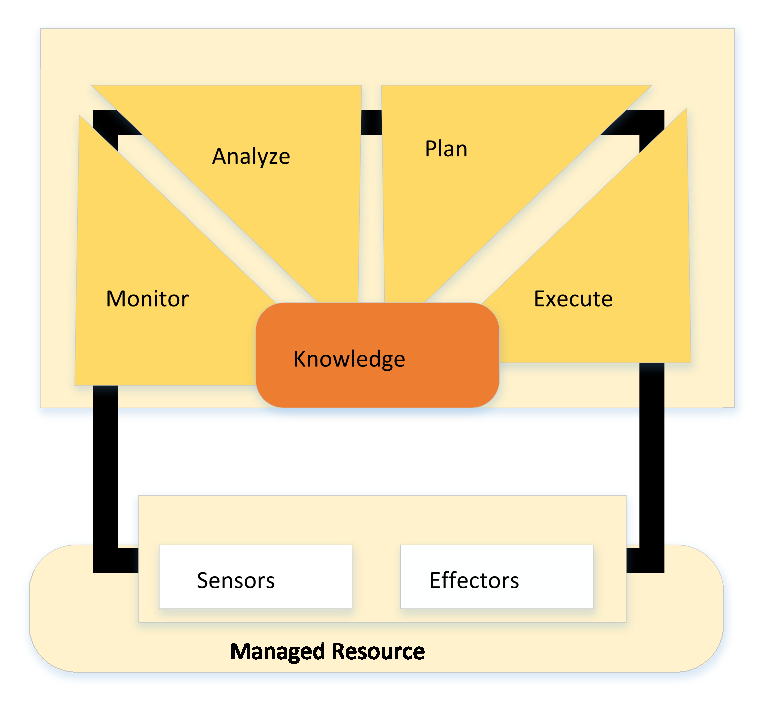
\includegraphics[width=0.45\textwidth]{image/mapeloop1.eps} 
	\caption[Architecture of autonomic management loop.]{Architecture of autonomic management loop suggested by IBM (adopted from \cite{mape-loop-pic}).} 
	\label{fig:mapeloop}
\end{figure}
  
 Components of the autonomic loop have a specific interpretation when viewed in the control theory context. 
 The following is an enumeration (description) of autonomic loop components considering control theory.
 % Below, we enumerate components of the autonomic loop and describe them in the context of the control theory. % Figure \ref{fig:control-loop} presents a schematic structure of such control loop.
 In a control theory sense, the goal of any optimal control loop is to choose a sequence of feasible \textit{control actions} over time that maximize a defined \textit{performance criterion} (or objective function)\footnote{One can instead say the optimal control minimizes an expected total cost function.}.


 \subsection{Monitoring Subsystem} The monitoring subsystem is responsible for measuring inputs, and outputs of the managed system (system I/O in a control theory sense), quantifying system I/O, sometimes aggregating system I/O, and keeping system I/O as a history. In a closed-loop (or feedback based) control, the controller constantly considers the most recent monitored data for calculating the proper actions. 

 Several computer system performance metrics can be collected. For example, hardware level metrics for each host, operating system metrics (e.g. file, network, and memory management subsystems), process level metrics, and service specific metrics for specific types of server processes (e.g. load balancer, web server, application server, and the database server). In a batch-oriented system there are additional metrics, such as the average number of jobs in a queue or the average job's queuing time. There are existing tools for monitoring computer systems, such as
 \textit{Collectd}~\cite{collectd}, \textit{Nagios}~\cite{nagios}, Java Management Extensions (JMX)~\cite{jmx}\nomenclature[A]{JMX}{Java Management Extensions}, and IBM Tivoli monitoring\cite{ibm_tivoli_monitoring}. 
  
   \subsection{Analyzer}
    The analyzer subsystem of the autonomic management loop, identifies and tunes a model of the system, and estimates the unobservable portion of the system state. The model enables the autonomic manager to project the system's behaviour and the state, from the current state under different actions.  A major concern is the ability to synchronize the model based on observed behaviour of the system. In our case, the analyzer is composed of a first principle mathematical model encoding the system's knowledge combined with statistical techniques to perform data-driven learning. 

 \subsection{Planner} 
 A planner uses the model to rapidly explore multiple decisions and find near-optimal solution \cite{litoiu_hierarchical_2005,aiber2004autonomic}. The search space is formed by the actions over time. The search for finding the proper actions can be based on a mathematical optimization in continuous space (e.g. methods such as primal decomposition, interior point methods, stimulated annealing, etc.) or can be a search in the discrete space (e.g. a combinatorial optimization).
  Whether the search is continuous or discrete, it is directed towards a goal or a set of goals.

\section{Optimal Control Theory}  
  In general, the goal of any optimal control approach is to choose the sequence of feasible control actions that maximizes a defined performance criterion (or an objective function) of the following form: 
 \begin{align}
   & \underset{u_0,...,u_{T-1}} {\text{minimize  } }  \lim_{T\to\infty}  \frac{1}{T} E\left[\sum_{t=0}^{T-1} g(x_t,u_t) \right]   \label{eq:general-control-problem-1} \\ 
   & x_{t+1}=f(x_t,u_t)+w_t  \label{eq:general-control-problem-2} \\ 
   & h(x_t,u_t)  < 0 \label{eq:general-control-problem-3} 
  \end{align}
  
  where $x_t$ is the system state,
  $E[\ldots]$ denotes the expected value,  
  $u_t$ is the controlled input, 
  $w_t$ is the uncontrolled stochastic input, 
  $T$ is the control interval, 
  $g$ is the (non)linear stage cost function, 
  $f$ is the (non)linear state transition function which maps the current state to the next one,   
  $h$ is the nonlinear function defining the limits of possible inputs and states.      
  Equation \ref{eq:general-control-problem-1} denotes that the objective is to minimize the overall cost, from the current time step to infinity (i.e. infinite horizon control), by choosing the optimal control inputs. The equation \ref{eq:general-control-problem-2} is called the process model and determines how the system state moves from one step to the next. 
  The inequality \ref{eq:general-control-problem-3} defines a set of possible state-input combinations at any given time. For example, if at state $x_1$ input $u_1$ is allowed, then $(u_1,x_1)$  will be in the set representing the $h$.   
  
In a feedback based scheme or a \textbf{closed loop control}, at any given time, the controller makes its decisions (i.e., to allocate resources) based on the information available from the system up to that time. % and the information deduced and maintained by the controller itself.  
   The solution to the above optimization is obtained and applied at each step of the control. Thus, the original plan is adjusted according to the new observation samples of the environment from the previous step. This solution is called a control policy: 
  \begin{align}
  \phi_t=\mathbf{R^{(t+1)n}}\to \mathbf{R^{m}}   \nonumber \\ 
  u_t=\phi_t(x_0,...,x_t) \nonumber
  \end{align}
  where $n$ is the number of the state variables, $m$ is the number of the input variables, and $t$ is the index of the current time step.

Normally for solving this optimal control problem one must form a set of equations according to dynamic programming principles. For most cases, the dynamic programming is often quite challenging and impossible for large problems. 
%\begin{figure}[htbp]
%\begin{center}
%% \includegraphics{figure/global_view1} 
%\caption{default}
%\label{default}
%\end{center}
%\end{figure}
In the following subsections, we briefly summarize those control problems of interest that can be solved analytically or computed numerically with polynomial complexity. These control problems include linearized dynamic control, optimal linearized dynamic control, policy iteration in finite state models, heuristic policies, and model predictive control (MPC).   
 The proposed controllers vary in their architectural complexity; which depends on the existence of a model for the target system, the theory underpinning the model, and the usage (or omission) of an estimator to track hidden variables in the model. 

\subsection{Optimal Linearized Control}
\label{sec:optimal-linearized-control}       
In some control problems, the optimal control policy has static state feedback control form: $u_t=\psi_t(x_t)$. Using this policy, an optimal input at every step can be obtained from the current state (as opposed to the current and previous states $u_t=\phi_t(x_0,...,x_t)$). 
 For example, consider the Linear-Quadratic-Gaussian (LQG)\nomenclature[A]{LQG}{Linear-Quadratic-Gaussian} control problem:
 \begin{align}
   & \underset{u_0,...,u_{T-1}} {\text{minimize  } }   \lim_{T\to\infty}  \frac{1}{T} E\left[\sum_{t=0}^{T-1} l(x_t,u_t)\right]   \label{eq:linear-control-problem-1} \\  
   & x_{t+1}=Ax_t+Bu_t+w_t \label{eq:linear-control-problem-2} \\ 
   &  F_x x_t + F_u u_t < f  \label{eq:linear-control-problem-3}      
  \end{align} 
   Here the symbols $x_t$, $u_t$, $w_t$, $T$ have the same meaning as equations \ref{eq:general-control-problem-1} to \ref{eq:general-control-problem-3}; they subsequently denote the system state, control input, stochastic input, and system lifetime. 
   $l$ denotes the Euclidean (or second) norm function (i.e. $\|\boldsymbol{x}\| := \sqrt{x_1^2 + \cdots + x_n^2}$). 
$F_x$  and $F_u$ are convex functions of $x$ and $u$.
$f$  is a convex function.
Finally, $A$ and $B$ are matrices.  

The equation \ref{eq:linear-control-problem-1} denotes that the objective is to minimize the overall cost from the current time step to infinity (i.e. infinite horizon control), by choosing the optimal control inputs.  The only difference with \ref{eq:general-control-problem-1} is that here the stage cost function $l$ is quadratic.
Note that, the process model denoted by the equation \ref{eq:linear-control-problem-2}   has a linear form. Also note that, the set of possible state-input combinations, defined by the inequality constraint \ref{eq:linear-control-problem-3}, is guaranteed to be convex. 
  
 The solution (i.e. the control signal) for this problem, has a feedback form, and is itself a linear system called Linear Quadratic Regulator\cite{lqr}. It takes the output of the system under control ($y_t$) as input and generates the proper input to be applied to the system ($u_t$). 
% \hat_{x}=[A-LC-(B-LD)K]\hat_{x}+Ly
% u=-K\hat_{x}
% or 
% in discrete time you just get x and apply this on it 
 Internally, this controller is based on a dynamically adjusted LQ-optimal gain applied on the \textit{state estimate} driven from an estimator. 
 % in discrete time http://www.mathworks.com/help/control/ref/dlqr.html 
 The estimator in LQG is usually a simple or an extended Kalman filter~\cite{welch_introduction_1995} \nomenclature[A]{EKF}{Extended Kalman Filter} able to maintain a good estimate of model unknowns by calibrating itself to measurements during runtime.
 Note that the LQG solution is only optimal for the linear dynamic systems with Gaussian noise, quadratic objectives and no constraints. 
   
   % In this solution, function $mu$, which maps every state to an optimal action, is identified by a LQ\nomenclature[A]{LQ}{Linear Quadratic.} optimal gain and is obtained by directly solving the associated Riccatti equation. 

\subsection{Policy Iteration}  
When the model underlying the system is Markovian with finite states $X$, the problem of finding an optimal policy that maximizes a long-term cost function, has a solution; investigated under the umbrella of Markov Decision Processes (MDP)\nomenclature[A]{MDP}{Markov Decision Process}. 
Computing the optimal value function and policy requires solving a nonlinear system of equations. When the underlying state of the system is hidden (Hidden Markov Model or HMM)\nomenclature[A]{HMM}{Hidden Markov Model}, which is usually the case, solving the problem is not quite so simple. The solution can then be investigated as a Partially Observable Markov Decision Process (POMDP)\nomenclature[A]{POMDP}{Partially Observable Markov Decision Process}. Unlike LQG, in a POMDP, there is no separation principle. Meaning that, one cannot estimate the state distribution and perform optimal control on the known state.\footnote{In LQG the state distribution is Gaussian, and thus, the mean value can be easily used for projecting to future.}
 The solution, in this case, is to pick a policy format and gradually improve the stationary policy using the observed result of the controller. The \textit{policy iteration algorithm} generates a sequence of improving stationary policies. Similarly, the \textit{value iteration algorithm} is then used to converge iteratively towards an optimal cost $J^*$. 
 
 \subsection{Sub-optimal Control}
 There is a small set of problems for which the optimal control policy with a feedback control form can be computed.  However, sub-optimal feedback solutions are extremely common. 
  For example, consider a linear system which is mathematically modelled as: 
  \[ x_{t + 1} = Ax_{t} + Bu_{t} \] 
  where $u_{t'}$ are the control inputs and $x_{t'}$ is the system state. 
  In the \textit{linearized dynamic control}, one should suggest a small or efficient set of control inputs $u$ that transfers $x$ to $x_\text{target}$. %considers the 'state transfer' of a linear system    
 Similarly, a regulation problem involves taking the system output ($y_t$) to a reference output or a set-point ($y_\text{target}$). Assuming the control error is the difference between the current system output and the desired output ($y_\text{target}$): $e_t=y_t-y_\text{target}$, it is desired that control error be transferred to zero.
  % A proper control signal (here allocation actions) is calculated based on control error, where  
        
  A feedback loop for this purpose can be constructed by feeding back the control error (the difference between a set-point and a measured output) as an input to the system (often with some intermediate processing). 
For a system whose dynamics are known
\footnote{The dynamics of a system can be represented in several mathematical forms such as transfer functions, state-space models, difference equations, etc. Depending on the form used, the controller might be designed using the same mathematical method (e.g. a transfer function).}(e.g. through system identification techniques), a proper feedback based regulator can be designed to make the system output achieve a degree of the following properties:  
(i) responsiveness to an error, 
(ii) the degree to which it overshoots the set-point, 
(iii) the degree of oscillation. 
    
For a system whose dynamics are known (e.g. through system identification techniques), a proper controller can be designed using the design techniques such as pole placement, root locus, etc. The model used during system identification can take several forms such as transfer functions, state-space models, difference equations, etc.
 
%\subsection{Steady-State Equivalent Problem} 
%Sometimes the optimal control problem can be converted into a deterministic optimization based on system's steady-state behaviour. In this case, a new \textbf{steady-state equivalent problem} is constructed and solved.   A steady state equivalent problem can be obtained by substituting mean-values with the same $f$ regardless of time index. 
%For example, in case of LQG (equations \ref{eq:linear-control-problem-1} to \ref{eq:linear-control-problem-3}), steady-state equivalent problem is as follows: 
%  \begin{align}  
%   & \underset{\bar{u}} {\text{minimize  } }  l(\bar{x},\bar{u}) \\
%   & \bar{x}=A\bar{x}+B\bar{u}+\bar{w} \\ 
%   & F_x \bar{x} + F_u \bar{u} < f
%  \end{align}
% variables $x_t$ and $u_t$ are considered to have constant values denoted by $\bar{u}$ and $\bar{x}$ and the process noise $w_t$ is considered to have a constant value equal to its mean $\bar{w}$. 
%
%   In the general case of control problems (i.e.  equations \ref{eq:general-control-problem-1} to \ref{eq:general-control-problem-3} ),  the problem has to have certain properties  in order to be   transformed into an equivalent steady-state  form; for example, when $w_t$ is separable from process dynamics and system inputs (i.e. $x_t=f(x_t,u_t)+w_t$) and noise has a certain distribution. 
%  % Note that the structure of $f$ is preserved. 
%
 \subsection{Model Predictive Control (MPC)} 
In Model Predictive Control (MPC) (also referred to as Limited Lookahead Control or LLC)\cite{abdelwahed2004control, kandasamy2004self}\nomenclature[A]{LLC}{Limited Lookahead Control}, the controller explores a search space formed by different choices of control actions over a predicted model \cite{bhat2006enabling} to find an optimal solution; thus, a management problem is posed as a sequential optimization under uncertainty. 
The search space includes a set of future states within a lookahead horizon. Controller then selects a path that minimizes a cumulative cost while satisfying both state and input constraints within the lookahead horizon
$u^*_j|j\in [t , t + N-1]$. 

In a Certainly Equivalent Controller (CEC) implementation, at each time step $t$, one
 makes a set of forecasts $\hat{w}_{t|t} ,\ldots,\hat{w}_{t+N-1|t}$ for future steps based on the observed state trajectory $x_{0},...,x_{t}$. 
% in fact, the only way in which capital Xt comes into this is through $\hat{w}_{j|t}$
 % the observed state trajectory $x_{0},...,x_{t}$ is irrelevant, except in $x_{j+1}$. 
 Then one is simply going to use these forecasts in the following optimal control problem as if the forecast were perfect. The first control input leading to this path is chosen as the next control action.
\begin{align} 
    \underset{u_t,...,u_{N+t-1}} {\text{minimize } }  &  \sum_{j=t}^{t+N-1} l_t(x_j,u_j) + l_{t+N}(x_T)  \label{eq:mpc-control-problem-1}   \\ 
    \text{subject to: } 
    & x_{j+1}=A x_{j}+B u_j + \hat{w}_{j|t} & j=t...t+N-1  \label{eq:mpc-control-problem-2}   \\
    & u_j\in U_j   & j=t...t+N-1  \label{eq:mpc-control-problem-3}  
\end{align}        
 Here $u_t,\ldots,u_{N+t-1}$ are variables and $x_t, \hat{w}_{t|t} ,\ldots,\hat{w}_{t+N-1|t} $  is the known data. The symbol $x_t$ has the same meaning as equations  \ref{eq:linear-control-problem-1}  to \ref{eq:linear-control-problem-3}; it denotes system state at time $t$. $N$ is the length of the lookahead window, $\hat{w}_{j|t}$  is the prediction of future disturbance $w_{j}$ at time $j$. $u_j$ is the future control input at time step $j$. $l_t(x_j,u_j)$ is a quadratic function representing the stage cost at time step $t$. $l_{t+N}(x_T)$ is the cost of deviation of the terminating state $x_T$. $U_j$ is the input constraint at future time $j$.  

 There is a common misconception about model predictive control, that the quality of the derived control inputs only depends on the quality of the predictions.  However, this is not true. In MPC, one forms a prediction of what the future disturbances $\hat{w}_{t|t} ,\ldots,\hat{w}_{t+N-1|t}$ are going to be, based on the observed state trajectory $x_{0},...,x_{t}$. These predictions can be just the mean value of the disturbance (i.e. as opposed to conditional expectation), or they can come from an external analyst. No assumption regarding the correctness of the forecasts is necessary for CEC to work.  In most cases, not one of the $\hat{w}_{j|t}$ will actually come true; despite this, the approach works very well in practice. In fact, if all $\hat{w}_{j|t}$ were true, then the problem would be a deterministic optimal control (as opposed to stochastic control problem). %  while reducing the cost of solving such  stochastic model predictive control problems, to linear with the horizon size.  


%  \subsection{Emergent Behaviour}   
% In \textit{Emergent Behaviour Approach}, autonomic systems can be built based on naturally occurring emergent systems (e.g. flocking\cite{spector2003emergence}, ant colonies \cite{camorlinga2004emergent}, and market economy \cite{kephart2001software,tesauro_utility_2004,eymann2003self}). Complicated patterns can emerge from the interplay large number of autonomous entities that behave according to some simple rules \cite{turing1952chemical, gierer1972theory}. Feedback and reconfiguration can be done in these systems by incorporating evolution through the concept of death or failure (cells die, market actors loose money).  
%
%
% As an example of these systems, virtual markets, composed of numerous simple actors interacting with money, can be used to build complex goal-oriented decision support systems \cite{cheliotis2003autonomic}. For example, in a resource allocation problem in grid infrastructure \cite{foster1997globus,foster2002grid} market-based control can be applied to remove unwanted resource contention. \cite{montresor2003messor} showed how an ant algorithm could be used to solve the problem of dispersing tasks uniformly over a network. Similarly, the Routing Information Protocol (RIP)\nomenclature[A]{RIP}{Routing Information Protocol})  routing table update protocol uses simple local rules that result in good overall routing behaviour. Other examples include autonomous grid scheduling protocols \cite{kreaseck2003autonomous} and peer-to-peer file sharing networks [gnutella, stoica2001chord].  In all of these systems the whole has a functionality more than the sum of the parts.

%
% Assume the Grid manager has to decide about the hosts that should handle tasks based on the resources left on the host (i.e. central processing unit (CPU), network and disk interfaces, and data storage) and the nature of the tasks. In market-oriented approach, one can assign tasks to autonomous entities and letting these entities find a suitable host. Autonomous entities have to use electronic currency to purchase the resources necessary to complete its task. Based on the resource usage at hosts, market determines prices for that host (i.e. congestion results in high prices). Less congestion through even spatial distribution of agents will follow naturally as agents choose hosts with lower prices. Temporal load balancing will be also resulted from the fact that some agents wait until prices drop. 
%


   \section{Cloud Computing}
   % \section{Service Center as a Queuing Network}    
 A Large Scale Software Center (LSSC)\nomenclature[A]{LSSC}{Large Scale Software Center} aims at large scale delivery of on-demand computational power (specifically network storage, computational devices, and services) to a user community.   
 \footnote{Ultra Large Scale systems (ULS)\nomenclature[A]{ULS}{Ultra Large Scale systems}, is a closely related term coined by researchers at Carnegie Mellon's Software Engineering Institute, referring to a system composed of a large set of systems with a variety of stakeholders communicating and operating to satisfy separate (possibly conflicting) goals.}
Current examples of such system include grid computing~\cite{foster1997globus,foster2002grid} and cloud computing~\cite{BHayesACMComm2008,MArmbrustEtAlTR2009,BRochwergerEtALIBM2009,RBuyyaEtAlFGCS2009}. 
    
Grid computing, having arisen from the high-performance computing (HPC)\nomenclature[A]{HPC}{high performance computing}  community near 2000, targets the delivery of on-demand computational power using a unified network of loosely coupled computers in the form of ``super virtual computer". The aim of designers was to let users plug their own programs into the infrastructure, and use resources for a desired duration. 
Current implementations of computing grids usually target long-running resource intensive applications (or jobs) that are submitted by a few users. Examples of these applications are distributed simulation \cite{ddsos,ddsos2},
scientific visualization \cite{wolf2002smartpointers}, 
continual queries \cite{babu2001continuous,kumar2005resource}, 
video conferencing \cite{huang2003network}, 
and transcoding \cite{radiantGrid}.  

Cloud computing is another manifestation of LSSC that, according to many, has caught on in mainstream enterprises.
In the cloud, there is usually a clear distinction between a provider and a customer, and the extent of sharing is governed by economic rules and pricing (usually pay-as-you-go). 
In cloud computing, large condensed data centers, possibly operated by multiple stakeholders, are offered at different levels of abstraction (e.g. infrastructure (IaaS), platform (PaaS) and software (SaaS)) on-demand as commodities to a large community of users. While IaaS focuses on offering virtualized hardware, PaaS hosts applications composed of services, which make use of other infrastructure services. In PaaS, usually a specific programming language and API for infrastructure services is enforced. 
In SaaS, there is a more customized set of APIs for specific types of applications (for example, accounting), shared by all applications of that type. 
 
  The cloud model we consider in this thesis is composed of a set of applications, offering services that are used by end-users. The end-users are usually service consumers around the globe accessing the services through Internet Protocol (IP), and most often Hypertext Transfer Protocol (HTTP). End-users, in our cloud model, are divided into a set of classes, where each class has a certain population and behaviour (in terms of accessing the cloud resources).
  The services are either generic and offered by the cloud provider (such as naming, storage, etc.) or application-specific and developed by cloud consumers. Both services are hosted and administered on the available infrastructure. % The multiplicity of application services is a lot more than the cloud services. 
 Some services developed by the consumers are frontend, meaning that they are the first point of interaction with the end-user, other services are backend, meaning that they are invoked by frontend services.   
  
     In our cloud model, the relationship between classes and applications is one-to-one:  (i) each class uses the limited set of services offered by a single application (ii) there is only one class of users associated with each application.  
     Thus, in this thesis, we can use the concepts of an application and class of users interchangeably. 
    
\section{Service Centers as a Layered Queuing Models (LQM)}  
\label{sec:layered-queuing-models-introduction}   
Queuing theory based models \cite{petriu_approximate_1994,petriu_approximate_2004,badidi-queuing-2005} and Layered Queuing Models (LQM) \cite{rolia_method_1995,ramesh_multi-layer_1998} developed upon Mean Value Analysis (MVA)\nomenclature[A]{MVA}{Mean Value Analysis} of queuing networks have been used to capture the behaviour of multi-tier distributed applications \cite{litoiu_hierarchical_2005, xu_performance_2006,hamoun_ghanbari_tuning,liu_layered_????}. 
Queuing Models can be utilized to describe the expected performance of service centers (i.e. response time and throughput) in relation to various inputs. In the following subsections, we review the components of the queuing models.  

\subsection{Workload} 
\label{sec:workload-background}  
  In this section, we review workload parameters derived from a workload characterization, including workload intensities and service demands.    
 
 \subsubsection{Workload  Intensities}  
 \label{sec:workload-intensities-background}  
 Software components hosted in the cloud can be categorized %from workload point of view into services and standalone programs. 
 Workload of a service is driven by its external users but workload of a standalone software component (such as a simulator or a batch data processor) is controlled by itself or its data.  
 Both types of software components can be generalized as one. 
 In the first case, the workload is specified as a \textit{number of users} or a \textit{request rate}, and in the second case it is usually specified as a \textit{multiprogramming level} (the number of simultaneous threads running on behalf of a process) or an \textit{execution frequency} (the frequency that a specific software module is called).   
 The number of users for a service is equivalent to the multi-programming level and the user request rate is equivalent to the execution frequency.
   
 In general, the workload component can be modelled as either {\it closed} or {\it open}. In the open model, customers are assumed to make requests on average every $\tau$ seconds, independent of when they receive responses for the previous requests. The open workloads are identified by an average request inter-arrival time ($\tau$)\nomenclature[M]{$\tau$}{Workload's average request inter-arrival time}, which is measured in seconds, or an arrival rate ($\lambda$)\nomenclature[M]{$\lambda$}{Workload's average request arrival rate}, which is measured in requests per seconds. Often, these models assume that the arrival rate ($\lambda $) is a homogeneous Poisson process, and that inter-arrival times ($\tau $) are exponentially distributed with parameter $\lambda $ (mean of 1/$\lambda $).  
In a closed model, clients are assumed to wait for responses to their requests.  Upon receipt of this response, the client spends some time determining the next action before issuing a further request. Closed models are defined by the number of users ($N$\nomenclature[M]{$N$}{Workload's average number of total users}) and average think time ($Z$\nomenclature[M]{$Z$}{Workload's average customer think time}). The think time is considered to have an exponential distribution.

A service center may offer a large number of services where each service is used by more than one group of users. Each group of users may consume the services and the resources in a different way (for example, with highly different CPU demands). Thus, it is common to refer to each group as a different \textbf{class}. In multi-class models, outputs are given in terms of the individual customer classes. It is, therefore, reasonable to model each application with a separate class
of users. In the case of open multi-class models (with say $C$\nomenclature[M]{$C$}{Number of customer classes in the workload} customer classes), workload intensity is denoted by $\lambda\equiv(\lambda_1 \dots \lambda_C)$, where $\lambda_c$, is a class $c$\nomenclature[M]{c}{Index of a customer class} arrival rate. A closed multi-class model consists of $C$ classes, each of which has a fixed population. We denote the workload intensity by $N\equiv(N_1 \dots N_C)$ and by its think time $Z\equiv(Z_1\dots Z_c)$, where $N_c$\nomenclature[M]{$N_c$}{Number of users in class $c$} is the class $c$ population size, and $Z_c$\nomenclature[M]{$Z_c$}{Think time of class $c$} is the class $c$ think time. 

 \subsubsection{Workload demand: Interaction with Resources}  
 \label{sec:workload-demands-background}  
 A service and an application can be modelled by a set of queues, where devices are mapped to queuing or delay centers. CPU is the main resource consumed by programs.  Other resources such as hard disks and network are used from CPU. The programs accessing system resources are modelled as the customers of the queuing network. By modeling the cloud workload as a queuing network model, the general Mean Value Analysis (MVA) can be used to calculate the performance characteristics of the system. 
 
  In queuing models, service interaction with hardware resources is quantified in terms of service times.  The service time $D_{s,k}$\nomenclature[M]{$D_{s,k}$}{Service time of service $s$ at resource $k$ per visit to the service} is the time each request spends on a resource type $k$ when accessing service $s$. 
  For example, \texttt{view cart} service that is executed on an application server could be  characterized by the following  parameters: $D_{\mathtt{view cart},\text{CPU}}=30 \text{ ms}$, $D_{\mathtt{view cart},\text{DISK}}=30 \text{ ms}$. 
  Here, we assume the basic operations performed at the device when executing the service by the various  classes are the  same; thus, it is  reasonable  to  assume  that  the  average  service  times across classes are nearly equal.   
 %% Under common scheduling policies such as first-come-first-served (FCFS) scheduling all customer classes $c$ have
 % In a service-oriented system, the service demand $d_{c,s,k}$\nomenclature[M]{$d_{c,s,k}$}{Service demand of service $s$ of class $c$ at resource $k$ for a single visit to the service.} is the sum of all service times on resource type $k$ during one execution of service $s$ of  class $c$ ; thus it is indexed by the service $s$, the class $c$ and the resource $k$. 
     However, it is possible for different customer classes to require different total numbers of visits to the service center ($V_{c,s}$)\nomenclature[M]{$V_{c,s}$}{The visit ratio of class $c$ to service $s$. Or total direct and indirect mean requests to a service $s$ for one request from a user class $c$}, thus providing distinct service demands (which we denote by $d_{c,s,k}$):
     \begin{align} \label{eq:new-demands} 
       d_{c,s,k}= V_{c,s} D_{s,k} 
     \end{align}
     here $V_{c,s}$ is the \textit{visit ratio} of class $c$ to service $s$. It represents the total direct and indirect mean requests to a service $s$ for one request from a user class $c$\footnote{If $V_{c,s}$ is normalized (i.e. $\sum_s V_{c,s}=1$) then accesses to the $S$ services fall into a distribution referred to as the \textit{Web Interaction Mix}. For example, TPCW benchmark specifies two web interaction mixes: ``One is intended to simulate a workload where there are few buy orders and the majority of the customer requests are browsing the website. This is accomplished by having 95\% of the web pages accessed be the browsing pages, (Home, New Products, Best Sellers, Product Detail and Search pages) while only 5\% of the Web accesses are to the order web pages. This mix tends to place more pressure on the front-end Web Servers, Image Servers and Web Caches. The second mix is intended to simulate a website with a significant percentage of order requests. This is accomplished by having 50\% of the web page accesses be the browsing pages and 50\% of the accesses be to the order web pages. The second mix stresses the Database Server."\cite{tpcw_benchmark}}.  
  $d_{c,s,k}$ is the total service demand the service $s$ makes on a resource $k$
  %  (Possibly by several visits) 
  by a single request of class $c$\nomenclature[M]{$d_{c,s,k}$}{the total service demand made on service $s$, by a single request of class $c$.}. 
 % The actual number of accesses for a customer of each class can be represented in the model by appropriate values of the $V_{c,s}$ for each class $c$. 
 \subsection{Deriving Visit Ratios}    
 For some service-oriented systems, there is a systematic way to calculate  $V_{c,s}$ as follows: $V_{c,s}$ for front-end services can be calculated by Consumer Behaviour Model Graph (CBMG)\nomenclature[A]{CBMG}{Consumer Behaviour Model Graph}\footnote{CBMG is presented as a state transition graph in the workload characterization process.}  \cite{menasce2004composing}. 
    For backend services $V_{c,s}$ are obtained using the visit ratio of front-end services, and \textit{call multiplicities}  on the edges of \textit{service call graph}. 
       %:cite  the paper composing Web services: a QOS view
      A service call graph is an acyclic directed graph where each edge represents the number of calls from a caller service to a callee and each edge is annotated by a call multiplicity. 
    % 
Using the call graph one can calculate the visit ratios.
Let $\servMeanReq_{es}$\nomenclature[M]{$\servMeanReq_{es}$}{Mean requests made directly from any service $e$ to service $s$} be the mean requests made directly (i.e. call multiplicity) from service $e$ to service $s$. 
 Formally, the \textit{visit ratios} satisfy the following equation:  
\[  \left\{ 
  \begin{array}{l l}
   V_{c,s}=\sum_{s'=1}^{S} V_{c,s'} y_{s',s} & \quad \text{where $s$ is a backend service}\\
    V_{c,s''}  \quad \text{is computed from CBMG}, & \quad  \text{where $s''$ is a front end service}
  \end{array} \right.\]

 Algorithmically, $V_{c,s}$ is calculated from the call graph $\servMeanReq_{es}$ using the following set of equations\footnote{Assuming there are no request cycles, $Y_{cs}$.}:  
 % For this purpose user class $c$ will be defined to have an entry numbered S + c, and yS+c,s is the mean number of requests made directly to entry $s$ for one user response. 
%
%setting $Y_{c,S+c} = 1$ for all $c$, and using:    
%$ Y_{c,c+S} ,  Y_{cs} = \sum_{e=1}^{\numService+\numClasses} Y_{ce} y_{es}  $. 
\begin{align} 
& con^0=\zeros_{\numService+\numClasses, \numService+ \numClasses} \label{eq: compute-adjacency-matrix}  \\
& con^{(i)}= con^{(i-1)}+ \servMeanReq^i  \text{ for } i \in 1\ldots \text{levels}   \nonumber \\ 
&V=con^\text{levels}_{1\ldots \numClasses, \numClasses+1\ldots \numClasses+\numService} \nonumber 
\end{align}  
where  $con^{(i)}$ represents the \textit{contact level} of services and classes at the $i$'th iteration, taking $\servMeanReq$ as the adjacency matrix and $\servMeanReq^i$ is the power of $\servMeanReq$, or in simple words it is the contact level of each node to its $i$'th further away node.  
% \textit{contact level} of any front-end service to a backend service. 
For example, if web service B and C provide services to A, and services B and C both use web service E, then the $con^2$ from A to E  is calculated as $y_{AB}y_{BE}+y_{AC}y_{CE}$.  

% The demand of user classes on software-hardware resources is calculated based on usage of the services by user classes, the internal usage of services by other services, and the hardware resource demand of the associated services. The steps for calculation are as follows:
     
 \subsection{Replication} 
 When services are replicated, multiple instances are deployed on multiple hosts. Each replica is indexed by $j=(s,h)$ where $s$ represents the service and $h$ represents the host for the replica. Here the load of the original service is distributed between the replicas.
 One can adjust the load on each replica by distributing the accesses to replicas in a desired proportion. This distribution can be modelled by changing the call multiplicities in the call graph in the edges between the callers and the callee service replicas, or by directly considering the call multiplicities in visit ratios $V_{c,s}$.  
  Note that in case of the replication, service demands between replicas are shifted based on $V$ as the equation \ref{eq:new-demands} can be written as:
  % the sum of visit ratios for replicas of the same service is preserved: 
   \[ d_{c,s,k,h}=  V_{c,s,h} D_{s,k} \] 
   \[V_{c,s} = \sum_h V_{c,s,h} \]
   Also according to \cite{menasce1999methodology} the average service demand for a class $c$ on a resource $k$ of a host $h$ can be obtained from the original service demands as follows: 
    %\[ d_{c,k}=\sum_s d_{c,s,k} \]  
   \[ d_{c,k,h}=\sum_s d_{c,s,k,h} \]  
 % For onote that according to equations ....  this will eventually change that demand on resources. 
 \nomenclature[M]{$d_{c,k,h}$}{The total service demand made by a single request of class $c$ on resource $k$ of host $h$.} 
  Here, it is assumed that service demands are independent of the class of service and the host where the service is deployed. Essentially, it is separating the servers and the resources such as CPU. 
%In this case the total number of visits on each resource type $\sum_{k\in \text{same resource}} V_{c,k}$ and  the service time on each replica $S_{c,k}$
% stays the same.  %(for example v1+v2=110). 
%  however, unless the service times of all the replicas  are identical there is no guarantee that  the total service demand is preserved after reconfiguration; Meaning that there is no  notion of preservation of  service demands.


%  \textbf{service demand itself  can be decomposed to } 
%  \textbf{service times} (S)  for each visit and \textbf{the number of visits} (V)  for each request. In a multi-class model the service time, denoted by $S_{c,k}$, is the average service requirement per visit of class c on resource k. From modeling point of view once a request acquires the resource, it remains at that resource for its service time. 
%  Similarity the service demand, denoted by $D_{c,k} $ is defined as average service requirement per request of class c on resource k.  Following relationship holds between the service demand and service time:$D_{c,k} = V_{c,k} S_{c,k}$,  where  $V_{c,k}$ denotes the number of visits per request of class c at resource K. Also throughput of class c at center k is defined as: $X_{c,k}=\lambda_c V_{c,k}$.
% 
% As an example if we observe a system for 8 minutes, and 160 requests of class c are handled during this interval, and the resource k has been busy in total for 2 minutes to handle class c request then the service demand is $D_{c,k}=2*60/160=0.75$. 
%and if 400 visits has occurred for class c requests to resource k, then $D_{c,k}=2*60/400=0.3$. 
%
%In this type of formulation two things are important: 
%1st,  is one wants to project the behaviour of the system to a configuration that resource K is substituted with a faster one, he can divide the service demand of all the classes on that resource  by the factor that the speed is increased.  
% 2nd,  


  \subsection{Solution Techniques for the Closed Queuing Networks }   
 % For example, algorithm \ref{algorithm-open-queuing-solution}, adopted from \cite{lazowska_quantitative_1984}, represents such solution for open model workloads on a flat queuing network.  
 The set of equations giving the mean value analysis (MVA) solution to the model for closed workloads is as follows: 
\begin{align} 
& X_c(\vec{N})=N_c(\vec{N})/(Z_c+\sum_{k=1}^K R_{c,k}(\vec{N})) \label{eq:queuing-model1} \\
& Q_{c,k}(\vec{N})=X_c(\vec{N}) R_{c,k}(\vec{N}) \label{eq:queuing-model2} \\
& R_{c,k}(\vec{N}) = \frac{D_{c,k}}{\speedFactor_k} (1+Q_k(\overrightarrow{N-1_c})) \label{eq:queuing-model3} \\
& Q_k(\vec{N})=\sum_{c=1}^{C} Q_{c,k}(\vec{N})  \label{eq:queuing-model4}  
\end{align}  
 \nomenclature[M]{$X_c(\vec{N})$}{Average system throughput for class $c$ customers for workload $\vec{N}$} 
  \nomenclature[M]{$R_{c,k}(\vec{N})$}{Average delay for class $c$ customer at center $k$ for workload $\vec{N}$} 
   \nomenclature[M]{$Q_{c,k}(\vec{N})$}{Average number of class $c$ requests in resource queue $k$ for workload $\vec{N}$} 
    \nomenclature[M]{$Q_k(\overrightarrow{N-1_c})$}{Total queue length of resource $k$for predecessor workloads $\vec{N-1_c}$ with one class $c$ customer less than $\vec{N}$.}
    \nomenclature[M]{$\speedFactor_k$}{The speed factor of resource $k$} 
    Here, $X_c(\vec{N})$ denotes the average system throughput for the class $c$ customers for the workload $\vec{N}$.
  $R_{c,k}(\vec{N})$ denotes the average delay for the class $c$ customer at the center $k$ for workload $\vec{N}$.
   $Q_{c,k}(\vec{N})$ denotes average number of requests of the class $c$ in the queue of the resource $k$ for the workload $\vec{N}$.
    $Q_k(\overrightarrow{N-1_c})$ is the total queue length of the resource $k$ for the predecessor workloads $\overrightarrow{N-1_c}$ with one class $c$ customer less than $\vec{N}$. 
 $\speedFactor_k$ denotes the \textit{speed factor} of the resource $k$. 
 Here, the speed factor is used to standardize different resources in terms of the speed. This is to make the demands machine and application independent. Demand is described in terms of number of compute seconds for a standard CPU. Transferring a class's workload to different resources is assumed to preserve the standardized resource demand, although the final demand on the resource (i.e. $\frac{D_{c,k}}{\speedFactor_k}$) would depend on the resource's speed factor.  
% CPU work and call this the standard cycle. For example: a single clock cycle on one type of machine might do 1.1 standard cycles of work, while a single clock cycle on a less powerful type of machine does 0.8 standard cycles of work. 
 
   Efficient solutions can be obtained for the resulting set of equations by sequentially solving each equation for each workload $Q_{c,k}(N)$ based on predecessor workloads $Q_{c,k}(N-1_c))$; as opposed to simultaneously performing Newton step on equations written for all workload components. Another approximate fast solution is to substitute the following equation for equation \ref{eq:queuing-model3}. 
   \begin{equation}\label{eq:queue-length-rt}\begin{split}  
       R_{k}(N) &= D_{k}\left(1+\left[\frac{N_c-1}{N_c}Q_{k}(N)\right]\right)   \\
  \end{split}\end{equation} 
  One needs to initialize each $Q_{k}(N)=N/K$ for all $k$ and iterate through the formulas until the $Q_k$'s converge to a solution\footnote{Agrees to the last iteration within some tolerance (e.g., 0.1\%). }.  

%
% Here the first formula is the approximate arrival instant queue length at center $k$ seen by an arriving customer.  
% % When this algorithm terminates, the values of $R_{c,k}$, $X_c$,and $Q_k$ (all for population $N)$ are available.
%
%For a queuing network with $C$ classes and $K$ queuing centres, 
%computing a $Q_{c,k}(N)$\footnote{$N$ represents the number of users.} for all $c$ and $k$ involves solving $3 C.N.K +C.N+K.N$ simultaneous equations, with initial condition $Q_{c,k}(0)=0$. The equations are as follows:  
% ......
%   the equations represent 
%  exact arrival instant queue length at center $k$ seen by an arriving class $c$ customer, 
%   the service center residence time for each class, 
%  system throughput for each customer class, 
%  average number of customers of class $c$ in the queue of server $k$, 
%  and average number of customers of all classes in the queue of server $k$.
 
 \subsection{Software Contention and Layered Queuing Networks} 
  % Software Resources}   
 A method for considering software contention is to use the extensions such as the Layered Queuing Model (LQM) and the Method of Layers (MOL)\nomenclature[A]{MOL}{Method of Layers} \cite{rolia_method_1995}. In these models, software and hardware resources are mapped to separate networks of queues. The software queuing network \nomenclature[A]{QN}{Queuing Network} \cite{rolia_method_1995} (SQN)\nomenclature[A]{SQN}{Software Queuing Network} is constructed from the software call graph and hardware is derived from the computer architecture. 
 The way SQNs are derived from call graph is as follows:  
 \begin{enumerate} 
     \item For the software service that is not a critical section or is not governed by a thread pool there will be a delay centre in the SQN whose delay depends on the resources the service uses from hardware queuing network (HQN)\nomenclature[A]{HQN}{Hardware Queuing Network}. 
 \item For every critical section code (i.e. governed by a semaphore or a monitor) there is going to be a single queuing centre in the SQN.
 \item For every software resource governed by a thread pool there is going to be a multi-server in the SQN. 
  \item For every call between a software service $a$ and software service $b$, there will be a connection between the corresponding centres in SQN. Moreover, a call multiplicity is associated with every call.  
 \end{enumerate}
  
   The number of visits for every class and hardware-software resource is obtained by accumulating the call multiplicities as described earlier. The initial hardware-software service demands for each class is obtained by multiplying visit ratios and service times. 
The actual algorithm providing the solution to LQN is provided in chapter \ref{ch:appendix1} (appendix 1).  
  
  \subsection{Multiple Resources with a Shared Queue} %Resource Multiplicity
  Hardware and software resources with multiplicity (such as multi-core CPUs or even multiple identical CPUs with the same workload) are modelled with multi-servers. % A hardware multi-resource is represented by the number of identical single hardware resources that share the same queue. 
 % Hardware resources with multiplicity are used to denote 
  Multi-servers can be approximated with techniques introduced in~\cite{seidmann1987computerized,menasce1994capacity,lazowska1984quantitative} for load-dependent servers.  
    Multiplicities for software resource are used to model multi-threaded software where active threads of the thread pool are modelled as multi-resources, sharing the same request queue. Note that a single active thread case (i.e. a critical section implemented by a monitor or semaphore) is modelled by a single software queuing center with multiplicity of 1. 
  Also, note that the solution of the LQM with unlimited software resource multiplicity (i.e. thread pool-less or pass-through software modules) and unlimited hardware resource multiplicity (i.e. delay center) denoted by $RT_{c,\infty}$, is going to be sum of the  demands of software services invoked by each request of the class $c$ on the hardware resources: 
  \begin{eqnarray} 
 R_{c}^\infty=\sum_k R_{c,k}^\infty = \sum_k D_{c,k} 
  \end{eqnarray}  

  %  Also note that in hardware layer the resource utilization has a linear relationship with demand. In software layer, the demands are the associated response times from the hardware layer resources, and since the response time of the hardware layer has a non-linear relationship with the demands the software resource utilization has a non-linear relationship as well. 
  
	\subsection{Model Granularity and Modeling Complexity} 
	In this thesis we mainly associate queuing and delay centers in our models with computing resources of servers (i.e. CPUs). However, during the estimation process, the service demands capture a lot of details other than just the CPUs� processing rate or delay. 
	
	In a typical data center, there are far more elements than just server CPUs. Some of these elements are physical machine's RAM and hard drives, storage area networks, communication network switches (i.e. top of the rack and aggregate switches), and server caches. 	

	Although it is possible to model a large subset of these entities using queuing network models, this might not be useful in the later stages when one tries to estimate the model�s unknowns or optimize over controllable parameters of the model. 

	When each component of the data center is modeled using a separate queuing center, the estimation of parameters of such model becomes extremely hard. This is due to the fact that not all of data centers components provide measurements that can be used in the estimation process. For example physical level network links (i.e. wires), and data link layer Ethernet switches might not provide resource utilization information. This means that, we would not be able to know what percentage of the capacity of a physical wire is used or unused, and thus we have to incorporate this in the model as unknown parameters. 
		
		In our approach, each queuing center not only models the CPUs, but also abstracts a set of physical resources that the workload passes through while executing a specific service. For example, the delay of a queuing center that models a Web server, already includes the delay added by the physical machines hard disks, remote storage, or virtual memory management unit (which itself is affected by the amount of RAM). In conclusion, the demands of this queuing centers capture a lot of details that might not be limited to host CPUs.
		

%  \subsection{Expectation Maximization}. 
%
%  In cases which throughput measurements for some classes on some servers are missing (e.g. when per-class-throughput for backend servers is not available) the least squares method does not lead to a convex optimization problem.\footnote{ Note that if there is a classifier at the load balancer layer that tags the requests by their associated classes, then the throughputs per-class in front-end services are known. Also if there is a one-to-one relationship between classes of users and applications, then the requests on front-end services of applications are naturally tagged. However, this is not usually the case for backend services.}   
%
%  In this case, the data sequence should be estimated together with the hidden workload demand parameter. One way to approach this is through expectation maximization (EM) algorithm.  
%% the latent factors are intentionally included, and parameter learning itself provides a mechanism for knowledge discovery.
%
%%  We refer to z as hidden variables or latent factors.
%%   http://ai.stanford.edu/~chuongdo/papers/em_tutorial.pdf
%
%%  http://www.seanborman.com/publications/EM_algorithm.pdf 
%
%    As an example, let�s assume per-class throughput of the services over time 
%
%   $X_{c,s,1},\ldots,X_{c,s,T'}$ 
%
%   are missing but the total throughput of services over time $X_{s,1},\ldots,X_{s,T'}$ are available. Starting from some initial parameters, $\hat{D}^t_{c,k}$, we determine for each 
%
%  timestep $t'$ the per-class throughputs $X_{c,s}$ which were more likely to have generated the $X_{s}$. Then we assume these $X_{c,s}$ to be correct, and apply regular MLE to get $\hat{D}^{t+1}_{c,k}$; we repeat these two steps until convergence.
%
% 
%
% Note that the expectation maximization algorithm comes with guarantees only of convergence to a local maximum of the objective function (except in degenerate cases).
%
% Running the procedure using multiple initial starting parameters is often helpful; similarly, initializing parameters in a way that breaks symmetry in models is also important.
%
% 
%



  \section{Summary}  
   In this chapter, we reviewed the necessary theoretical background. We introduced the autonomic computing and the IBM's MAPE-K loop guideline.  We also reviewed the mathematics behind several types of controllers. Finally, we described the mathematics of performance models for modelling software and hardware components. We explained how, different applications are modelled using customer classes, and how services are modelled using queuing and delay centres. 
   
   


 


 \chapter{Related Work}      
\label{ch:state-of-art}    
%\begin{center}
%\textbf{This chapter contains material from Ghanbari et al. \cite{hamoun_ghanbari_exploring_2011,hamoun_ghanbari_tuning,ghanbari2014mpc,ghanbari_feedback-based_????}}.
%\end{center}

The chapter reviews the current state of the art for solutions to the IT service resource management problems introduced in chapter 1.   
The problem solutions reviewed include:
   (i) methods for reducing monitoring overhead and computational complexity of the Bayesian service demand estimation for service replicas,
   (ii) methods for improving the placement of service replicas in a private cloud using dynamic empirical models, and 
   (iii) methods for considering the reconfiguration cost, when modeling the optimal placement of the service replicas.
 
   Separate sections are provided which describe the related work for each (i-iii) of these problems. 

 \section{Service Demand Estimation}   
\label{sec:service_demand_estimation} 

Some early research into CPU demand estimation is described in \cite{menasce2008computing}.
  % this is just equation solving for each step separately, Computing Missing Service Demand Parameters for Performance Models
In this early work, missing service demands are computed by solving a set of nonlinear equations based on a queuing model. For each step, the following equations are solved:
 \begin{align}
 \underset{(d_{c,k})} {\text{minimize } }   & 
 || R_c-\sum_{k=1}^K \frac{d_{c,k}}{1-\sum_{c'=1}^C \lambda_{c'}d_{c',k}}||  \nonumber \\  % \sum_{c=1}^{C}  
 \text{subject to:}  \label{eq:simplistic_estimation} \\ 
 &  d_{c,k}>0  \text{  for each $c$,$k$} \nonumber \\ 
 & \sum_{c=1}^C \lambda_{c} d_{c,k} < 1 \text{  for each $k$} \nonumber
 \end{align}  
 where $R_c$ and $\lambda_c$ are known and $d_{c,k}$ are estimated.  
 To solve \ref{eq:simplistic_estimation}, Menasc{\'e} et al. use an iterative approximation algorithm that takes the estimated demands of the past step as the initial value for the estimates of the current step.

\cite{rolia_parameter_1995} and \cite{rolia_correlating_1998} used linear regression to predict the demands of running programs in a distributed system. Many approaches, such as \cite{pacifici_cpu_2008}, estimate service demands by solving the following linear Least Square Estimation (LSE) problem based on the utilization law %\ref{eq:utilization-law}: 
  \begin{align}     \label{eq:utilization_based_estimation}
    \underset{(d_{c,k})} {\text{minimize } }   ||U_{t,k} -  \sum_{c} X_{c,t}  d_{c,k}||   
  \end{align} 
 % $\ddot{\utilization_{h,k',t'}}  =  \sum_s \ddot{X_{s,h,t}} \hat{D_{s,k'}}$
%  Thus the solution for all centres can be obtained by: 
% \[ D =  ( \lambda^T \lambda)^{-1} \lambda^T U \] 
% \[ U_t=\sum_{c=1,...,C} \lambda_{c} D_{c,k} \]      
  here $U_{t,k}$ denotes the utilization of the $k$'th resource centre at time $t$, $X_c$ denotes the throughput of the customer class $c$, $d_{c,k}$ denotes the class $c$'s service demand on the $k$'th resource centre, and $||.||$  represents the second norm function. In the formulation \ref{eq:utilization_based_estimation}, it is assumed that the throughput values of all user classes and the utilizations of all servers are known over some time interval. It is also assumed that, the
  LSE is based on the utilization law and the assumption that residuals are independent and identically distributed (IID) noise with a Gaussian density (i.e. $N(0, \sigma^2)$): 
 \begin{align}
 U_{t,k} = \sum_{c} X_{c,t}  d_{c,k} + v_{t,k},\   t=1,...,T , k=1,...,K 
  \end{align}
 where $T$ is the length of a monitored time interval (or the number of samples), $K$ is the number of resources and $v_{t,k}$ is the residual associated with time $t$ and resource $k$.   

 References \cite{pacifici_cpu_2008,zhang_regression-based_2007} employ the multivariate linear regression technique for a one-tier network. However, \cite{zhang_regression-based_2007} focuses more on modeling inter-request dependencies of session-based systems and \cite{pacifici_cpu_2008} focuses on mechanisms to deal with issues such as insignificant flows, collinear flows, space and temporal variations, and background noise. 
 
 \subsection{Non-Linear Regression}
If response time metrics are available, the service demands problem can be posed as a nonlinear least squares estimation. 
  An example of research where regression splines are utilized is \cite{courtois_using_2000}. To find model parameters in nonlinear least squares problems, usually algorithms such as Levenberg-Marquardt \cite{wild_nonlinear_2003,dumouchel1989integrating} can be used. In \cite{dumouchel1989integrating}, for example, a weighted nonlinear regression is iteratively refined. Weights used in each iteration are based on observation residuals from the previous iteration. Points that are outliers are down-weighted, and their influence on the fit is decreased. Iterations continue until the weights converge. Note that, the convergence of the parameters and the correctness of the estimation depend on the underlying model. If applying maximum likelihood estimation (MLE) on the model does not follow a convex form, it is quite possible that the regression does not converge, or converges to an incorrect value.  % \cite{rolia_parameter_1995,zhang_regression-based_2007,rolia_correlating_1998}: 
% 
	In \cite{zhang_workload_2002} and \cite{liu_parameter_2006}, multi-class queuing models were used in a two-tier web cluster, to infer service times per-class at different servers using throughput, utilization, and per-class response time measurements. They try to minimize the sum of predicted response time mean square errors using a non-linear optimization solver and a quadratic minimization program. \cite{kraft_estimating_2009} also uses a combination of MLE and the queuing model for estimation.  

 References \cite{gmach_workload_2007,gmach_capacity_2007} claim to perform the demand prediction of enterprise workloads by discovering patterns, but the referred to demand is per-application not per-request; thus, they do not tackle the same problem as ours. 
 
   Despite simplicity and ease of implementation, the regression-based approaches have three major shortcomings:
   \begin{enumerate}
   \item  In the presence of missing measurements, the regression problem might not be a convex optimization. For example, in the case where measurements are simply throughput and utilization, if a resource utilization or a class throughput is missing, terms such as $X_{c,t}.d_{c,k}$ might make the optimization non-convex.   
% also an additional $T$ variables are added to the optimization. 
   \item  Even if the solution to the LSE problem can be formulated analytically (i.e. through algebraic operations on matrices), the computational complexity is still third-degree polynomial with respect to the number of samples $T$ and resources $K$: $O((T.K)^3)$. Thus, as the size of the regression window grows (i.e. to provide more accuracy), solving for a large-scale environment (cloud) becomes more computationally expensive.  
   \item There is no way to specify the rate of change in the unknown variables explicitly. The value of unknown demands is considered constant within the regression interval. As a result, the number of samples within each steady-state interval determines how quickly the estimated demands are going to change with time. With fewer samples, they will change more frequently and with more samples they will change less. 
     \end{enumerate}

    \subsection{Bayesian Approach}   
   %  The Bayesian posterior estimation was thoroughly described in \ref{sec:bayesian-estimation}.
		Papers \cite{woodside_use_2005,xu_performance_2005,zheng_tracking_2005} use Bayesian estimation to effectively deal with the problems of regression-based approaches enumerated earlier. They treat all unknown parameters as variables that vary over time. Thus, they can deal with the addition of a missing data measurement to unknown parameters without extra complexity. They also reduce the amount of computation by solving the associated problem analytically and deriving a filter for it (i.e. Kalman type). This filter greatly reduces the estimation cost by doing step-by-step computation based only on the measurements of the current step and the state of the previous step, thus reducing computations to $O((C\cdot K)^3)$. Using a Kalman filter, they also specify the rate of change of the unknown parameters by specifying the process noise and the measurement noise covariance matrices. 

        The only issue in using the Bayesian approach is convergence. Convergence requires that at minimum, we have more measured parameters than estimated ones. As will be discussed in chapter \ref{ch:estimation} in detail, this convergence condition either puts a limit on the number of classes whose demands are to be estimated or requires a considerable number of parameters to be measured. The major contribution of our approach is dynamic clustering of user classes, to minimize the number of unknown variables. Yet, we leave enough classes to satisfy the accuracy criterion.  

  To the best of our knowledge, the combination of dynamic clustering and performance model parameter estimation for multi-class models has never been investigated. The only close reference to our work in terms of the final goal is \cite{sharma_automatic_2008}. 
In \cite{sharma_automatic_2008}, Sharma et al. try to categorize requests based on resource usage characteristics. However, \cite{sharma_automatic_2008} ignores the prior knowledge about requests in the system and classifies the requests on-the-fly. Also, they use a machine learning technique called Independent Component Analysis (ICA). Of course, ICA will alleviates the need for server instrumentation, but might affect the accuracy due to not using the extra available information (i.e. of the classes of users).


\section{Application Resource Share Adjustment in Cloud Using Dynamic Empirical Models}      
\label{sec:application_resource_share_optimization_private_cloud}
 	%As examples of this contribution, \cite{li_fast_2009,li_performance_2009} attempt to find the minimum infrastructure cost deployment, subject to processing capacities and application SLAs. SLAs are described in terms of constraints on the average delay and throughput for each application.  
%\cite{li_sla-driven_2010} attempts to simultaneously minimize cost while maximizing QoS attributes, through multi-objective optimization or MOO. A Pareto-optimal solution can find a good trade-off between conflicting performance and cost-saving goals rather than finding a single global optimum~\cite{soror_automatic_2010}. Geometrically these well-balanced solutions concentrate around the ``knee'' of a multi-objective trade-off curve. 

Maintaining application level QoS guarantees has been the subject of much investigation. Recently satisfying the dual objectives of QoS guarantees and server consolidation in cloud computing environments has received considerable attention. Current approaches formulate the optimization problem in different forms.

One approach attempts to minimize cost subject to performance constraints
\cite{li_fast_2009,li_performance_2009}. In this approach, the SLA represents constraints rather than flexible goals. Constraints could be based on response time or throughput. For example \cite{li_fast_2009} finds the minimum cost deployment subject to processing capacity and user throughput constraints. It seeks deployments which minimize the overall cost of the hosts used, subject to meeting average delay and throughput constraints for each application as posed by its SLA. 

The second approach attempts to minimize cost while maximizing QoS attributes simultaneously, through multi-objective optimization or
MOO~\cite{li_sla-driven_2010}. For example, Pareto-optimal solutions can find a good trade-off between conflicting performance and cost-saving goals rather than finding a single global optimum~\cite{soror_automatic_2010}. Geometrically, these well-balanced solutions concentrate around the ``knee'' of a multi-objective curve.

 % The purpose of this work was to demonstrate the advantage of ``adaptive'' models relative to 
% ``static'' models in optimization.
The main difference between our approach and the related work is the use of dynamic empirical models (for each application) within the global optimization loop. These models update themselves at runtime in order to adapt to perturbations in the environment not captured in initial model specification.  This results in more accurate models being passed to the optimizer, allowing for better resource utilization on a global scale.  

% huse of the decomposed model for better convergence, a custom optimization routine, and the use of utility functions. The works \cite{li_fast_2009,li_performance_2009} find the minimum cost deployment subject to processing capacity and user throughput constraints. However, they assume a monolithic model has already been built.
% \cite{soror_automatic_2010} targets a Pareto-optimal solution, a good trade-off between conflicting performance and cost-saving goals. Also the idea of dynamically adjusting the resource shares of multiple applications in order to meet a specified level of service differentiation, was used in \cite{liu_optimal_2007} and \cite{lim_automated_2009}, although using adaptive multivariate controller and for a more limited scenario than ours (i.e. maximum one PM per application layer).
    
\section{Service Replica Placement Considering the Reconfiguration Cost} 
\label{sec:service_replica_placement_considering_trhing_cost} 
 Static or one step ahead optimizations are the main tool to target minimization of infrastructure cost for private clouds while meeting applications QoS guarantees. But, when one takes into account the cost of reconfiguration, one has to add the time dimension into the optimization. This makes the optimization very complicated, and this complexity should be dealt with using the proper method. The approach we take here is using the Model Predictive Control (MPC) framework.  

In terms of related work, there are only a couple of papers that target the same kind of problem.
Paper \cite{zhang2012dynamicPlacement} discusses the service placement in geographically distributed clouds through MPC. However, \cite{zhang2012dynamicPlacement} defers from our approach in two ways: (i) it uses a single class open queuing network model, which is much simpler than the closed multi-class model we use, and (ii) it derives an analytical solution to a SSEC version of the problem first and then targets this solution as a desired state through MPC, considering the
quadratic reconfiguration stage cost. In our case, this was not possible because we needed a sparse deployment at each step. From the same authors, paper \cite{zhang2012dynamicProvisioning} discusses controlling the optimal number of active servers for Google clusters where web applications and data processing jobs are both considered as generic jobs treated under scheduling policies. In this paper, they also use MPC, similar to our approach. They first found the optimal steady-state solution through a single class queuing model and then reached a solution considering the reconfiguration cost through MPC.

Other examples of using MPC in computing-resource management context are~\cite{baiefficient,abdelwahed2004control, kandasamy2004self, bhat2006enabling,patikirikorala2011hammerstein}; however, these examples do not target service placement.
In \cite{baiefficient,abdelwahed2004control,kandasamy2004self} MPC is used for managing web server power consumption by changing the frequency at which the CPU is operating. 
In this example, the number of choices of frequencies is quite small (i.e. less than 10 alternatives), changes in the frequency are trivial, and the feedback does not have a lot of delay. 
They were able to use a very small lookahead horizon and a simple model, and calculate the actual expected value of the cost over process noise ($w_j$) distribution, for every action path, without getting a state explosion.  
In \cite{bhat2006enabling} MPC is used to decide about the amount of data each node of a cluster should send through a set of data streams, and the amount to cache to disks. The proposed solution maximizes the throughput up to the network congestion point. In this paper the cost function was quadratic, which greatly aids with solving the MPC problem (heuristics not needed).   

  \section{Summary}   
 In this chapter, we discussed related work for the problems we introduced in chapter 1. The first problem we targeted is scaling up the EKF based estimation of service demands for large-scale service centres without increasing the monitoring overhead. Currently, there are two sets of techniques for service demand estimation:  regression-based approaches and Bayesian filtering approaches. The Bayesian approach addresses the existing issues with regression-based approaches, such as the ability to tune the expected rate of parameter changes over time.
 However, the Bayesian approach suffers from a lack of convergence when the number of missing data items and hidden parameters exceeds the number of monitored metrics. Our proposal improves the Bayesian estimation in terms of convergence. It reduces the proportion of unknown parameters and metrics to measured ones by grouping user classes, giving the filter a chance to converge with less monitoring overhead, and less computational complexity. 
 
 The second problem we target in this thesis is using dynamically tuning to improve the accuracy of the empirical models; we then trace this accuracy in the overall performance improvement in the allocation. We try to adjust the resource shares of a set of virtual machines that run on behalf of a set of applications. These VMs are deployed on a limited number of physical machines. The goal is to best satisfy the overall application performance, performance being described in terms of a set of utility functions. Our approach is based on point-wise stationary approximation (PSA) and solved for a set of the steps separately.
	   
	The third problem was the placement of services considering the reconfiguration cost. MPC is used to derive an optimal action at any time step based on the amount of workload to the services experienced to that point. This let us take the reconfiguration cost into account and minimize it.




 \chapter{Tracking Adaptive Performance Models using Dynamic Clustering of User Classes}
 \label{ch:estimation} 
%\begin{center}
%\textbf{This chapter contains material from Ghanbari et al. \cite{hamoun_ghanbari_tuning}}.
%\end{center}

  This dissertation uses a model to project the state of the system under different actions. 
	%  The modelling enables the controller to project the system's behaviour and state under different actions.  
 To do this projection, one needs to have the current state of the system in terms of the model elements. The objective of an estimator is to describe the system in terms of a given parametric model. This identification process includes finding or estimating the parameters of the model using the data obtained from the system, in an ongoing fashion.  
 
 In our case, the model corresponds to the cloud and the service instances, which run within the cloud. Thus, the identification mostly corresponds to the estimation of workload intensities (the number of users and the think times in a closed workload case and the arrival rate in an open workload case) and the service demands which are treated as hidden parameters of the model
\cite{
rolia_parameter_1995,
rolia_correlating_1998,
courtois_using_2000,
pacifici_cpu_2008,
zhang_regression-based_2007,
zhang_workload_2002,
liu_parameter_2006,
gmach_workload_2007,
gmach_capacity_2007}. 

  The estimation is carried out using the measured parameters of the system such as device utilizations ($U_{h,k}$), or class throughputs ($X_{c}$), and response times($R_c$), if available.
     For each measurement metric obtained from the monitoring subsystem, we have one or more relations according to the queuing theory. We use these relations in the context of the Kalman filtering approach.  
		
		
	  % --------------------------------------------------
  \section{Bayesian Estimation of Hidden LQN Parameters Using Extended Kalman Filter Estimator}    
  \label{sec:bayesian-estimation}  
   In the Bayesian approach, the probability estimate for a hypothesis is updated as additional evidence is learned; this makes Bayesian approach a good fit for estimation tasks on sequential data. One can look at performance data as a sequence of measurements, where the unknown performance parameters are changing parameters to be estimated from observations \cite{woodside_use_2005,xu_performance_2005,zheng_tracking_2005}.
   
   All parameters are taken as latent variables. So it is assumed that the parameters distributions also vary over time, and there exists a \textit{state-space model} that specifies the dynamics of latent variables and the relation among the latent variables and the observations. 
Assuming that one knows the state and the measurement noise covariance structures, one can estimate the model parameters by solving the associated optimization. 
Assuming Gaussian noise, subject to model and domain constraints, the estimation problem can be described using the following optimization expression:  
    % \footnote{Note that with the assumption that $x$ has multivariate Gaussian distribution, at any given point in time $\hat{x}_t$ and $P_t$ fully present the state vector distribution. This also applies to $\hat{x}_0$ and $P_0$.}
  \footnote{Note that, determining the optimal parameter estimates cannot be done using a weighted least squares optimization of the measurement residuals (i.e. $y_t - h(x_t)$) with respect to the model parameters $\theta$, since the process equation in the model is non-deterministic.} 
  
  
  
\begin{align*} 
 %  \label{eq:mhe-optimization} 
 % \nonumber \\     
 \underset{x_0,...,x_T}{\text{minimize }}  
   &  (x_0-\hat{x}_0)P^{-1}(x_0-\hat{x}_0)
 	 + \sum_{t'=0}^{T-1} w^T_t Q^{-1}_t w_t 
	 + \sum_{t'=0}^{T}  v^T_t R^{-1}_t v_t \nonumber  \\ 
    \text{subject to:} \nonumber \\   
    & \hat{x}_t=[\overrightarrow{\hat{d}_t},\overrightarrow{\hat{N}_t},\overrightarrow{\hat{Z}_t}]^T  \nonumber \\  
    & u_t=[\overrightarrow{\tilde{d}_t},\overrightarrow{\tilde{N}_t},\overrightarrow{\tilde{Z}_t},\overrightarrow{\tilde{\Omega}_t}, \overrightarrow{\tilde{\rho}_t}]^T  \nonumber \\   
    & z_t=[\overrightarrow{R_t},\overrightarrow{U_{h,k',t'}},\overrightarrow{X_{s,h,t'}}]^T  \nonumber \\   
    & x_{t + 1} = x_t+w_t \nonumber \\     
    & z_t = LQM_{\tilde{x}_t}(\hat{x}_t)+v_t  \nonumber \\
    &  d_{c,s,h,t}>0  && \text{  for each $c$,$s$,$h$,$t$}  \nonumber \\  
    &  0<U_{h,t}< 1 && \text{ for each $h$, $k$} \nonumber
\end{align*} 
%% One of the benefits of this approach is the fact that we can specify dynamics of the state transition explicitly. 
where 
 $t$ denotes the discrete time. 
 $\tilde{x}_t$ is used to represent the known portion of $LQM$ parameters such as multiplicity of resources at time $t$. In other words, every value of $\tilde{x}_t$ defines a function of $x_t$, denoted by $LQM_{\tilde{x}_t}$. 
 $w_t$ is the process noise with a normal distribution, zero mean, and the covariance of $Q_t$ (i.e. $N(0,Q_t)$),  
 $v_t$ is the observation noise with a normal distribution, zero mean, and the covariance of $R_t$ (i.e. $N(0,R_t)$).  
 $x_t$ is the state to be estimated, composed of unobserved LQM parameters, with the mean of $\hat{x}_t$ and covariance matrix of $P_t$ (i.e. $N(\hat{x}_t,P_t)$).
 %For example, for two classes $\{c_1,c_2\}$, one service $\{s_1\}$ and one host $\{h_1\}$, the state can be:  
   %\begin{align} 
  %x_t=[d_{c1,s1,h1,t'},d_{c2,s1,h1,t'}, X_{c1,s1,h1,t'},X_{c2,s1,h1,t'}]^T  \label{eq:two-class-state-vec}  
 %\end{align}  
 %$z_t$ is the observed data vector that is output of the model.  
 $z_t$ is the vector representing the measured performance.  
 $LQM_{\tilde{x}_t}(\hat{x}_t)$ is, in this case, the observation model based on the queuing theory formulas \ref{eq:queuing-model1} to \ref{eq:queuing-model4} and it is non-linear with respect to the state vector.   
  % For example, in case of missing throughput values per classes, the state vector becomes: $x_t=\{D_{s,k',t'}\} \cup \{X_{c,s,t'}\}$.   

%\begin{figure}
	%\centering		
	%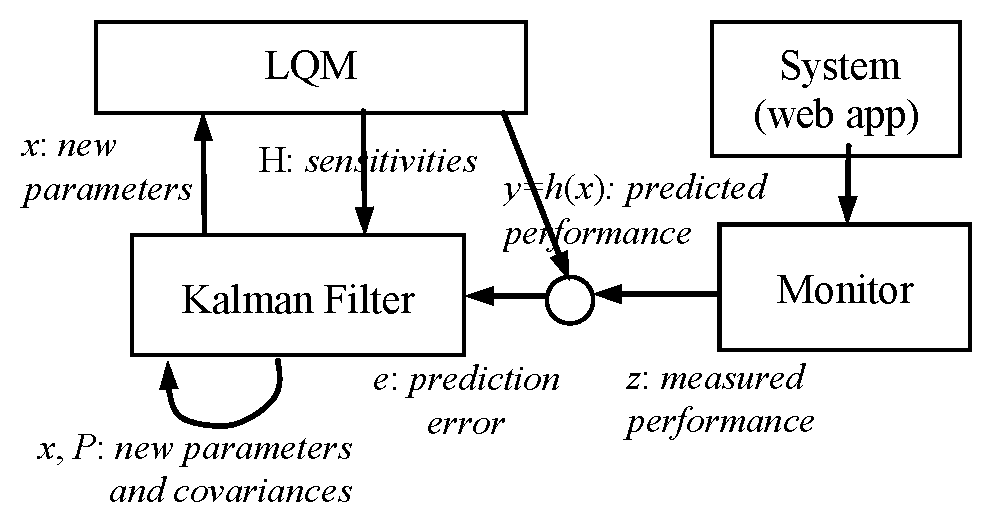
\includegraphics[width=0.8\textwidth]{image/image-tracking-structure.eps}  
	%\caption{Architecture of feedback based estimation using the extended Kalman Filter.} 
	%\label{fig:fig1}
%\end{figure}  
 The solution to the above optimization can be derived by an Extended Kalman Filter (EKF) \cite{zheng_tracking_2005}, a variant of the Kalman filter \cite{brookner_tracking_1998}. 
%Figure \ref{fig:fig1} depicts the architecture of this extended Kalman filter. Let $x$ and $z$ be vectors representing the parameters and measured performance, respectively. The model maps $x$ to an output vector $y$ (i.e., $y=h(x)$) which represents the predicted performance. The filter then estimates $x$ (which is not directly measurable) based on the observed performance $z$. 

 Assumed prior knowledge of the filter includes distribution of the initial state, and process and measurement noise structures: 
\begin{equation}\label{eq:filter-initial-state}\begin{split}
  \hat{x}_0  \\ %. I added the hat later on
  P_0&=E[(x-\hat{x}_0)(x-\hat{x}_0)^T]  \\
  Q_t &= E[w_t w_t^T]  \\
  R_t &= E[v_t v_t^T]  \\ 
 \end{split}\end{equation}   
 where
   $\hat{x}_0$ is the initial estimate,
    $P_0$ is the initial error covariance matrix, and 
   $Q$ and $R$ are the covariance matrices for the process and measurement noise, respectively.
  
%\begin{minipage}{\linewidth} 
The filter computations are recursive, beginning from an initial estimate $\hat{x}_0$, and an initial error covariance matrix $P_0$.
Each recursive step can be summarized as follows: 
\begin{enumerate}
\item  The core filter calculation is the update of the state estimate $\hat{x}_t$ and error covariance estimate $P_t$ by the linear feedback equation:
 \begin{align} 
& H_{t} = \left . \frac{\partial h}{\partial x } \right \vert_{\hat{x}_t^-,u} \\
& K_t  =P_t^- H_t^T (H_t P_t^- H_t^T+ V_t )^{-1} \\ 
& e_t   = z_t  - LQM_{\tilde{x}_t}(\hat{x}_t^-)  \label{eq:observation-error} \\  
& \hat{x}_t = \hat{x}_t^- + K_t e_t   \\
& P_t=P_t^- - K_t H_t P_t^-       
 \end{align}
\item The filter then projects the state estimate $\hat{x}_t$ and the error covariance matrix $P_t$ forward one step:  \begin{align}
  % \hat{x}_{k+1} = F(\hat{x}_t,u_t) 
 & P_{t+1}^-  = AP_tA^T+Q \\
 & \hat{x}_{t+1}^-=\hat{x}_t
 \end{align} 
\end{enumerate}
%\end{minipage}

 Here, $e_t$ denotes the prediction error vector obtained from the current modelled and observed output vectors ($LQM_u(\hat{x}_t^-)$ and $z_t$ respectively), and $P_t^- $ denotes the value of $P_t$  at time $t$ given measurements up to time $t-1$ (i.e. $P_{t|t-1}$).  
 $H_t$ is the matrix of sensitivity values or partial derivatives of the model function (i.e. $LQM_{\tilde{x}_t}(x_t)$) with respect to the parameters at their current values $x_{k}$,  whose $j$th column is the derivative of $LQM_{\tilde{x}_t}(x)$ with respect to $x_j$. 
 Essentially, this Extended Kalman filter (EKF) [25] linearizes $LQM_{\tilde{x}_t}(x_{t-1})$ by a first order Taylor series around the state estimate and does not take linearization errors into account. 

 Also note that here we assumed the process model chosen to describe the state is a ``random walk."  In this scheme the system state $x_t$ (here demand and workload) is assumed to evolve due to random drift $w$ as: $x_{k+1}= x_t+ w_t$. This means that a minimal assumption is made during the estimation of hidden parameters of this model: that the covariance matrix for $w_t$ is known (we denote it by $Q_t$). 
 Usually the covariance matrix is diagonal since workload components (number of users and think time) and user demands are assumed to change independently. The values are sometimes set according to $Q_{i,i} = \alpha  x_0(i)$, where $x_0(i)$ is the initial value of the $i$-th state variable to be estimated, and $\alpha$ is the ratio of expected changes for $x_i$'s,  (e.g. 0.02) with respect to their initial values.   

 The optimality and the convergence properties of the Kalman filter depend on the way the functions are linearized around the current estimate of x.   
  % Even the simple throughput and utilization measurement case solved with LSE, in the presence of missing throughput-per-class measurements, becomes non-linear with respect to the state vector. For example, assuming state vector  $x_t=[d_{c1,h1,t'},d_{c2,h1,t'}, X_{c1,h1,t'},X_{c2,h1,t'}]^T $, the utilization law $U_{h,t'}=\sum_c X_{c,h,t'} D_{c,h,t'}$, which is linear with respect to $c_{c,h,t'}$,  is non-linear with respect to state vector $x_t$:  $ U_t(x) = x_{1,t'}x_{3,t'}+x_{2,t'}x_{4,t'} $.   
	% --------------------%
	% these are just added
		The approximated $H$ matrix and the equations of the filter depend on the following three factors: 


  \textbf{The required estimates.} 
  The main estimates to be discovered are the service demands, and most of the time, the user population ($N_c$) and think time ($Z_c$) of each class. In this chapter, we assume that each service replica is identified by a subscript $j=1...J$ which summarizes a tuple $(s,h)$  (see the chapter 2). In other words, a replica $j$ is implicitly associated with a host $h$ and a service $s$. So a demand $d_{c,s,h,k}$ (introduced in the chapter 2) is re-written as $d_{c,j,k}$.  $d_{c,j,k}$ represents the service demand of a class $c$ at a replica $j$, on a hardware resource $k$. This is done to associate the variables exclusively to the unknowns and reduce the total number of variables. If there is no replica of a service $s$ placed on a host $h$, there will not be any variable $d_{c,j,k}$ defined for its estimated value. Note that the Kalman filter does not provide a way to enforce the equality constraints such as $d_{c,s,h,k}=0$ during estimation. So, one needs to substitute such variables with the associated constants.   

  \textbf{The measured parameters.}
     Usually the throughput of each class of users ($X_c$) can be easily obtained. The mean utilization of each resource type $k$ (e.g. CPU, disk, and network) on each host $h$ ($U_{h,k}$) and the mean response time for each user class ($R_{c}$) are also usually available. % for one req 

     \textbf{The missing data items.} On certain occasions, a subset of metrics from a subset of servers might be missing. For example, it is usually not feasible to get response time metrics from individual service replicas ($R_{c,j}$) without code manipulation or instrumentation. These missing data items are also treated as variables in our model.  
% Assume all the information captured from the real system, is summarized in a measurement vector $z$.  In the perfect information case $z$ would be: $z_t=[R_{h,s,t'},...,U_{h,k,t'},...,X_{s,h,t'}]$. 
%where $J=\left\vert{\{j=(s,h)|\theta_{s,h}\neq 0\}\right\vert}=\text{count}(\theta_{s,h}\neq 0)$ 


	 
\section{Dynamic Clustering of User Classes}  
  An important issue in using the Kalman filtering approach is convergence. The necessary and sufficient condition is given by the identifiability condition \cite{tanizaki_nonlinear_1996,wan_unscented_2000,welch_introduction_1995}. The convergence requires that at minimum, we have more measured parameters than estimated state parameters: i.e., 
   \begin{align}  
   \text{dim}(x) \leq \text{dim}(y)    \label{eq:identifiability}
    \end{align}    

 As we know, the estimated parameters might include:   
  (i) the demand of each class, on each service replica, on each resource ($d_{c,j,k}$), 
  (ii) the mean think time for each class ($Z_c$), 
 (iii) the number of users in each class ($N_c$).  
 
	  
 Thus $\text{dim}(x)$, based on the number of classes ($C$), the types of resources available in each server ($K$), and the number of service replicas in the deployment ($J$) is as follows\footnote{The dot sign was used to represent the multiplication.}:                
 \[ \text{dim}(x)=C\cdot J\cdot K +  C + C = C\cdot (J\cdot K+2) \]
 
In the case of $K=1$ (i.e. only one resource type), we have: \[\text{dim}(x)=C\cdot (J+2)\] 

 Note that in reality, the services can be classified into two kinds: the application-specific services, and the generic services.
   The relationship between classes and application specific services is a sparse one; meaning that there is a small number of application services used exclusively by each class of users. On the other hand, the relationship between the classes and the generic services is very dense because almost all the classes make use of some primary core services. 
   This sparsity and uniqueness, which constitutes an N-to-1 relationship between application services and classes, is a great help when it comes to estimation of the demands on user services. 
 In a sparse deployment, the term $C\cdot J\cdot K$ will be hugely decreased due to the fact that not every class $c$ makes use of a service replica $j$. 
 
  The measured parameters are most likely the mean response time and throughput of each class and the utilization of each server. If we also have a number of other measurements denoted by $\phi$ (for example the response time of each class at a service replica gives us another $C$ measurements) it results into: \[ \text{dim}(y) = \phi+2C + H\]  and the identifiability condition \ref{eq:identifiability} reduces to:
 \begin{align}  
 & \phi+2C + H \geq  C\cdot (J+2)  \\  
 & H+\phi \geq C\cdot J \\ 
  & C \leq H/J+\phi/J
  \end{align}    
   thus $\text{dim}(x)> \text{dim}(y)$, if $C$ is reduced to at least $(H+\phi)/J$. 
 Note that replicas are at least equal to the utilized hosts ($H\leq J|U_h>0$). So, the main factor is the number of extra measurements at the service replicas (i.e. $\phi$).  
For each additional class beyond $H/J$, we need an additional $J$ measurements. 
This linearly increases the monitoring overhead.
We should, therefore, keep the number of classes small, if possible. 

%\subsection{aggregation semantics}     
%Suppose the tensor $d$ assigns a value to every triple $<c,s,k>$. 
% Remember that $d_{c,s,k}=V_{c,s}D_{s,k}$. In order to make the number of unknowns smaller than dimensions of the tensor $d$ must be aggregated into a set of clusters.     
%In the rest of this section we propose a combination of clustering algorithm and bayesian method for effective grouping of classes. The clustering uses the K-means algorithm. 
%convergence: start from 1 class and go up until it does not converge because it is too many unknowns 
%Accuracy: how to measure accuracy? from the optimization. Every number of clusters corresponds to a different cost function (see \ref{eq:mhe-cost-function} ) and consequently different minimization problem, and different optimal trade-off curve.  Thus the measure of accuracy is actually the tradeoff curve or the $J$ that is achieved. f  
%Suppose there are $L$ services (i.e. $i=1,\dots,L$) in the system. 
%Let $R_{c(i)}$ be the predicted mean response time of class $c(i)$ requests. 
% we would like to have $C^0$ initial clusters in the system (i.e. $c=1,\dots,C^0$)
%

%\subsection{Dynamic Clustering Algorithm}
%\label{sec:dynamic-clustering-algorithm} 
In this section, we first discuss the modelling error due to clustering and then present an algorithm to determine the best choice of the number of clusters $C$ and the grouping of classes into these clusters.

\subsection{Modeling Error} 
\label{sec:modeling-error} 
Suppose the original $C$ classes (i.e. $c=1,\dots,C$) are reduced to $C'$ classes (i.e. $c'=1,\dots,C'$), and $c'=\psi(c)$ where $\psi$ is the function that maps the class $c$ in the original model to $c'$ in the new model. Let $R_{\psi(c)}$ be the predicted mean response time of class $\psi(c)$ requests. For the case of no clustering (i.e., each class in the original model is treated as a separate class in the new model), let ${R(C)}_c$ be the mean measured response time of requests for the original class $c$. Then a modeling error measure $E(C')$ for a new model with $C'$ classes is given by: 
\begin{align}    
	E_\psi(C')=\sqrt{\frac{1}{C}\sum^C_{c=1}{{\left(\frac{{R(C)}_c-\ R_{\psi\left(c\right)}}{{R(C)}_c}\right)}^2}}
		%=\textcolor{red}{\boldsymbol{\left|\left|\boldsymbol{\frac{R(C)-R_\psi}{R(C)}}\right|\right|}}
		\label{eq:modeling-error}     
\end{align}  

The hypothesis is that the error $E(C')$ tends to decrease when the number of clusters is increased. However, finding the clusters and the multi-class performance model associated with the clusters is complex, as $E$ is also a measure of how well the results from the filter and the model fit the measured data.




\subsection{Dynamic Clustering Algorithm} 
\label{sec:dynamic-clustering-algorithm-sub} 
Our classification algorithm is shown in Algorithm \ref{algorithm-estimation}.  Inputs to this algorithm are the LQM, a measurement vector $z$ and an error threshold $A$. The vector $z$ can include workload elements $\overrightarrow{\lambda_c}$ or $(\overrightarrow{N_c},\overrightarrow{Z_c})$, the measured response time $\overrightarrow{R^\text{m}_c}$ and throughputs $\overrightarrow{X^\text{m}_c}$, and the total utilization of the servers $\overrightarrow{U_h}$. The algorithm generates the best values of the number of classes (i.e. $C'$) for the new model, the grouping of original classes into these  classes (i.e. function $\psi$), and the service demand estimates for the service replicas (i.e. $d_{c',j,k}$, $\forall j\in\{1, \dots,J\}$, $\forall c'\in\{1, \dots,C'\}$, $\forall k\in\{1, \dots,k\}$).


\begin{algorithm}
	\small
	\SetAlgoVlined
	\SetKwInOut{Input}{input}
	\SetKwInOut{Output}{output}
	\SetKwInOut{Initialize}{initialize}
       \SetAlFnt{\tiny}

\Input{LQM, $z$, $A$}

\Output{The best choice of the number of clusters $C'$, aggregated demand ($d_{c',j,k}$) and mapping of old classes to new ones $c'=\psi(c)$. }

\BlankLine
$\{d_{c,j,k}\} \gets$ Estimate $d_{c,j,k}$, the service demand of class $c$, service replica $j=(s,h)$, at resource type $k$, from measurement data ($\forall j=(s,h)\in\{1, \dots,J\}$, $\forall c\in\{1, \dots,C\}$, $\forall k\in\{1, \dots,k\}$) using the model with no clustering; and set $C' = 1$.
\BlankLine 

\Repeat{$E(C') < A$}{
$\psi_{\{d_{c,j,k}\},C'} \gets$ Cluster the services based on the $d_{c,j,k}$'s into $C'$ clusters. 


$\{d_{c',j,k}\} ,\{R_{c'}\} \gets$ Estimate the parameters
$d_{c',j,k}$, the service demand of class $c'$ at replica $j$, at resource type $k$; solve the LQM with $C'$ classes and obtain results for $R_{c'}$, the mean response time of class $c'$ ($\forall j\in\{1, \dots,J\}$, $\forall c'\in\{1, \dots,C'\}$, $\forall k\in\{1, \dots,k\}$). 
\BlankLine

$E(C') \gets$ Calculate the modelling error  \BlankLine 

%If $E(C') > A$, then increase $C'$ by $1$ and go to Step 2. 
Increase $C'$ by $1$
\BlankLine 
}
Return $C'$, $\psi$ the original classes $c'$ associated with each cluster $c'$, and
$d_{c',j,k}$ ($\forall j\in\{1,\dots,J\}$, $\forall c'\in\{1,...,C'\}$, $\forall k\in\{1, \dots,k\}$ ) 
\BlankLine

\caption[The algorithm for estimation of service demands and clustering of user classes.]{The algorithm for estimation of service demands and clustering of user classes.}
\label{algorithm-estimation}
\end{algorithm}

In our investigation, the workload is time varying. The autonomic control loop is executed at regular intervals. If the modeling error of the existing grouping configuration is less than $A$, only the regular estimation is performed using the Kalman filter. On the other hand, if modelling error is greater than $A$, our clustering algorithm is invoked to obtain a new clustering of classes such that the modelling error becomes less than $A$ (see algorithm \ref{algorithm-estimation}). 

The clustering algorithm starts by estimating the service demands of all the service replicas from the measured response times using the original model with no clustering (Step 1). The estimation at this step is done by using either an Extended Kalman filter or the linear or non-linear least squares methods described in chapter 2.
Note that this is different from the estimation that is done at each step. The purpose of this estimation is solely for clustering the classes. 
If an EKF is used, the convergence criteria should be considered, and extra measurements should be used if necessary.  One can use the least squares method, taking the demands constant over the past few steps (moving horizon estimation format or MHE) to avoid the need for extra measurements. The necessary condition for this case is to have the estimation horizon wide enough to contain enough data points for the least squares method.   

In Step 3, the K-means clustering algorithm \cite{kaufman_finding_1990,likas_global_2003} is used to perform an unsupervised grouping of the service demands. K-means has low complexity and is adaptable to the continuous nature of our problem. Moreover, it is able to detect clusters in an efficient way, which does not require computing the distance of all the points to one another. K-means takes as input the number of distinct clusters to generate ($C'$) and will determine the size and members of the clusters (mapping between the classes and the clusters) based on the demands. 

The modeling error $E(C')$ is calculated at Step 5 using the $R_{c'}$, that was obtained in Step 4. If $E(C')\le A$, the algorithm terminates and returns (i) the best choice of the number of clusters, $C'$, (ii) the classes assigned to each of the $C$ classes, $\psi$, and (iii) the estimated service parameters for the different classes $d_{c',j,k}$ (see Step 7). 
 If the modelling error $E(C')$ is larger than the acceptable error $A$ (i.e. due to a gradual change in service demands over time) the algorithm increases the number of clusters and performs another iteration. Steps 3, 4 and 5 are then repeated to compute $E(C')$ for the new number of clusters. Note that a larger number of clusters would increase the measurement overhead and the computational cost of estimation, but it will decrease $E(C')$. 

\section{Experiment 1: TPC-W benchmark and FIFA98 workload}    
To show the applicability of the method, we performed our first experiment on the estimation of service demands of the TPC-W benchmark \cite{garcia2003tpc} implementation. We deployed the Java implementation of TPC-W \cite{volker_turau_tpc-w_????} with some modification, on a cluster of four Tomcat web servers and one single MySQL database server, with Linux as the operating system. 

TPC-W is an e-commerce web application composed of 14 URLs, namely 'admin confirmation, admin request, bestsellers, buy confirm, buy request, registration, home, new product, order display, order inquiry, product detail, search request, search result, shopping cart'.  Each of the URLs has a different service demands on web and database servers. 

The application also comes with a workload generator, which takes as input: (i) the number of users over time and (ii) a Customer Behavior Model Graph (CBMG), given to the workload generator as  a transition probability  matrix of a Markov chain. This workload is generated using Emulated Browsers (EB) whose behaviour and navigation is controlled by the Markov chain.  

The number of users over time are derived from FIFA98's workload \cite{arlitt_workload_2000}\footnote{The reason we chose FIFA98's workload over some other workloads commonly used in computing systems performance community (e.g. Google Workload Traces \cite{reiss2011google}) is that the workload includes very detailed information about access patterns of a web application by online users. Basically the workload is the detailed log of Apache web servers.
Google Workload Traces is mostly concerned with the amount of time it takes it Google cloud to complete a job and the performance of the scheduling. The trace also includes hardware level information about the resource usage on the physical machines. }.
This workload reflects variations that servers might experience at runtime. We picked a portion of the day 21's workload (see Figure 6), extracted the web pages, lowered the number of requests by the factor of 2 (to factor in our smaller scale deployment topology), and finally used Little's law \cite{little1961proof}  (i.e. $N=X(R+Z)$) to convert the obtained throughput ($X$) to the number of users ($N$) and think time ($Z$) used by the emulated browsers of TPC-W. We assumed that the FIFA98 website had maintained the same response time over the sampling period. % We then used the obtained number of users to the TPC-W benchmark using equal mix of buying, browsing, and ordering scenarios. 

 \begin{figure}[hp]
	\centering
		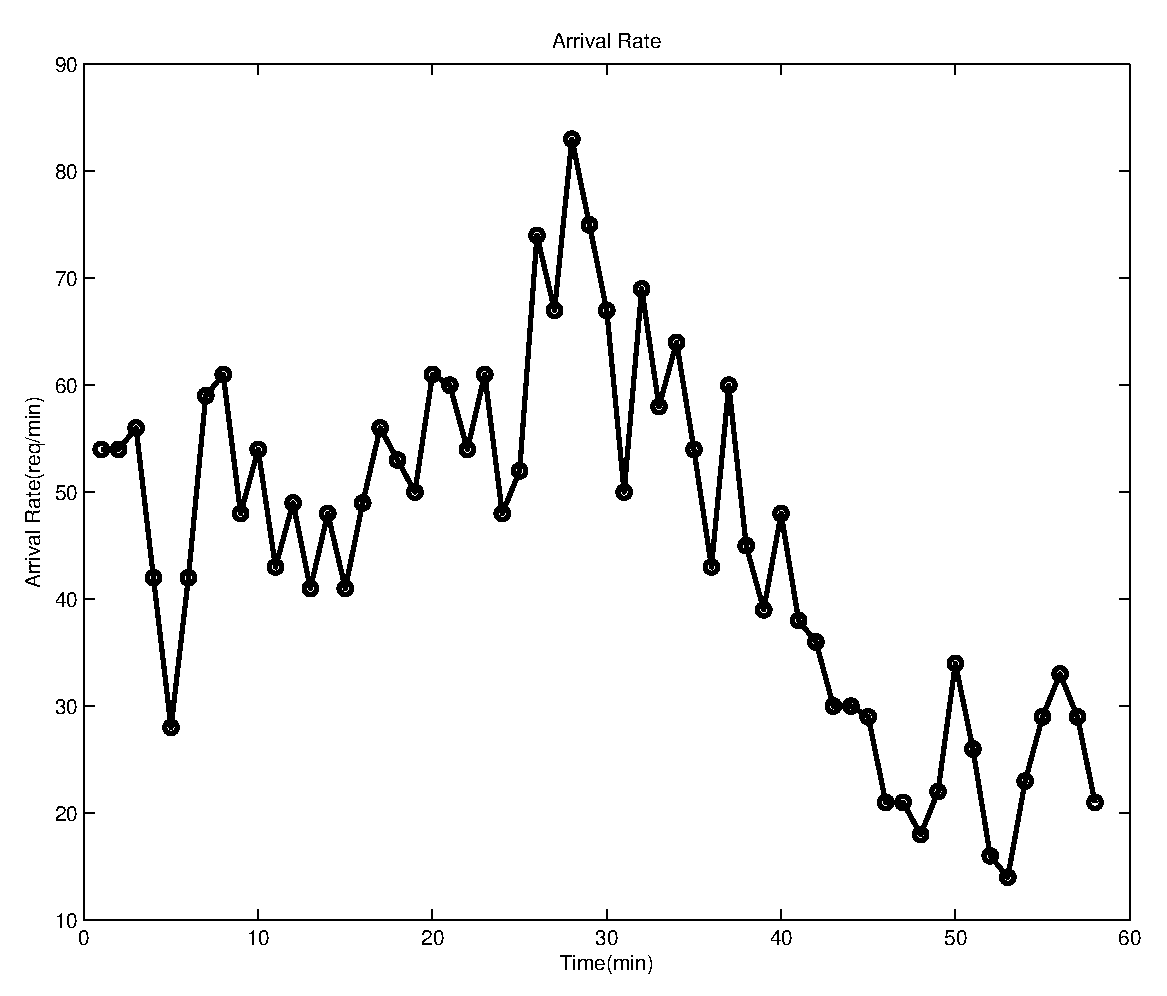
\includegraphics[width=0.7\textwidth]{image/workload-arr-rate.eps}
	\caption[FIFA98 workload, day 21, over an hour, used in demonstration of the estimation algorithm.]{FIFA98 workload, day 21, over an hour.}
	\label{fig:fig2}
\end{figure}
For obtaining data, we monitored one of the web servers and the database and logged data collected from one of the web servers and the database; these included: response times, throughputs, and utilizations. Each sample represented a minute of work, and the total length of the experiment was 1 hour resulting into 60 samples.

 \textbf{Estimation.} 
    The application was modeled as two services, web and database. Each service only has one replica placed on a separate server. We also took the users accessing the system through each individual URL as a class of users. 
    
		The average number of visits to web and database services are different for each class depending on the CBMG. This makes the average web and database service demands for each URL different, and subject to estimation. This leaves us with 28 parameters to estimate, 14 web service demands $d_{c,\text{w}}$ and 14 database service demands $d_{c,\text{db}}$. Note that there is only one service replica for each of the services in the system, each installed on a different host.
		
		The monitored metrics include the throughput and response time of each class (28 measurements) and the utilization of each server (2 measurements). Since number of measurements is already more than the number of unknowns (28 versus 30), the convergence criterion is met even with no clustering.

		Figure \ref{fig:estimated-demands-casestudy1} represents the estimated service demands for 13 classes for the web service. One service demand is removed from the diagram to increase the clarity. 
 \begin{figure}[htbp]
	\centering
	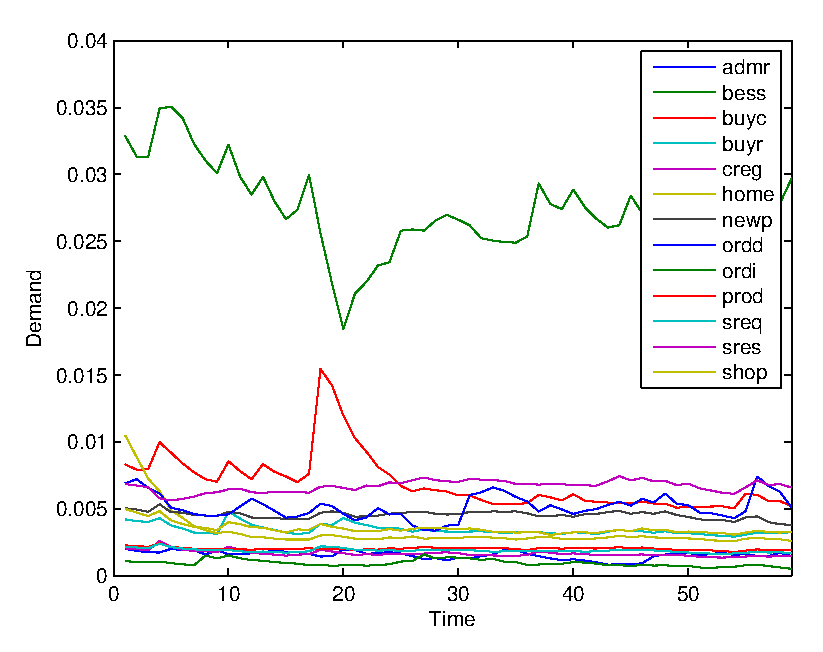
\includegraphics[width=0.7\textwidth]{image/demand13_estimated_kamlan.eps}
	\caption[A sample example of estimated service demand of 14 classes on a single service.]{Estimated service demand for 14 URLs on Web server service.}
	\label{fig:estimated-demands-casestudy1}
\end{figure}
Note that in the diagram the demands do not change frequently. We suspected that this is mainly because (i) the workload is unable to fully saturate the system or (ii) the combination of workload mixes are the same.
      
  Our analysis on this experiment had three parts. First, we ran the algorithm statically with a different number of clusters and measured the modelling error. In our evaluation, we used an expanded definition of the modeling error metric given by its average over the duration of the experiment (from $1$ to $T$): 
 \begin{align} 
 E=\frac{\sum^T_{t=1}{E(C')_{t}}}{T} 
  \end{align} 
where $t$ ranges over the estimation steps. $E(C)$ is the modelling error defined in equation \ref{eq:modeling-error} and $T$ is the number of estimation steps. 
\begin{figure}[htbp]
	\centering
	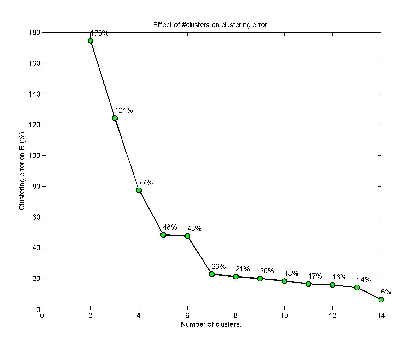
\includegraphics[width=0.7\textwidth]{image/modeling-error-vs-num-cluster.eps}
	\caption[The relationship between the modeling error and the number of clusters.]{Modeling error decreases with the number of clusters.}
	\label{fig:modeling-error-decreases}
\end{figure}

 As we expected, the error decreased while we increased the number of clusters (See Figure \ref{fig:modeling-error-decreases}). The experiment also shows that modelling the system with one or even two classes introduces a large modelling error and that modelling with an intermediate number of classes (8, for example) might give us an acceptable modelling error. 
\begin{figure}[htbp]
	\centering
	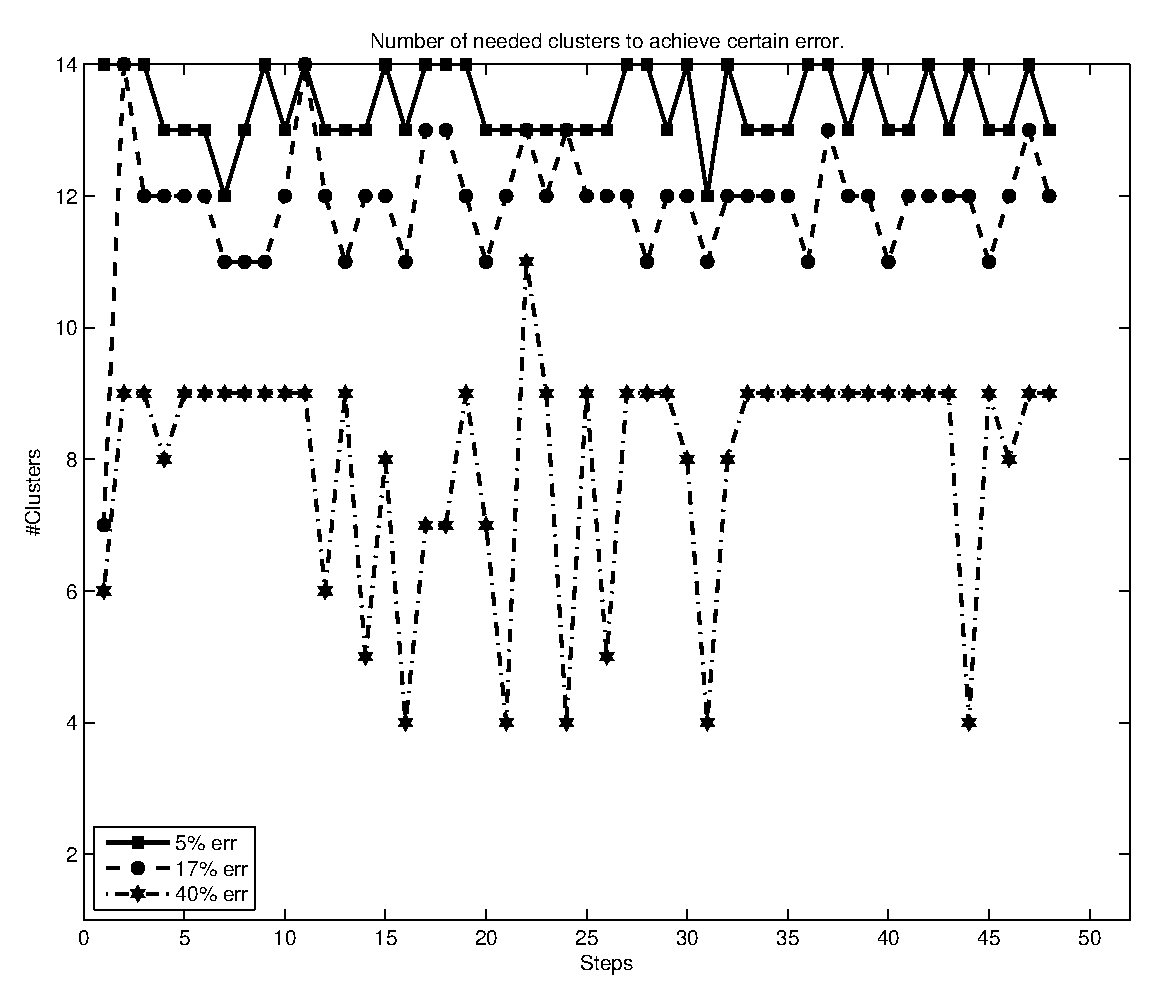
\includegraphics[width=0.7\textwidth]{image/cluster_num_by_error.eps} 
	\caption[ The minimum number of clusters, dynamically adjusted, to reach a certain modeling error.]{The minimal number of clusters needed to reach a specific modeling error threshold.  We can reach 40\% and 17\% error, consecutively using 9 and 12 clusters on average. In order to reach 5\% error, we have to perform full clustering.}
	\label{fig:minimal-number-needed-clusters}      
\end{figure}

In the second part, we applied our estimation and clustering algorithm to find the minimal number of needed clusters to reach a certain modelling error. The algorithm is applied at each sampling period and, as a result, the clusters change dynamically. As Figure \ref{fig:minimal-number-needed-clusters} shows, we can reach 17\% error using between 7 and 12 clusters for the duration of the experiment. For a modelling error less than 40\% we need 9 clusters on average. In order to reach 5\%, there are sampling periods in which we need maximum number of classes, which is 14.

In the third part of the analysis, we observed the correlation between the \textit{within cluster sum-of-squares} (WCSS) for demands and the modelling error achieved using the estimation and clustering algorithm. We chose 140 different groupings. For each number of clusters, we generated 10 random combinations. This let us navigate all possible WCSS's that could result from different groupings. Figure \ref{fig:cluster-sum-of-squares} shows that, on average we experienced a larger modelling error for the clusters with higher WCSS errors. In other words, the modelling error is minimized, whenever the WCSS is minimized. As a result, our assumption is validated since K-means is exactly the algorithm to minimize the WCSS. 
\begin{figure}[h]
	\centering
	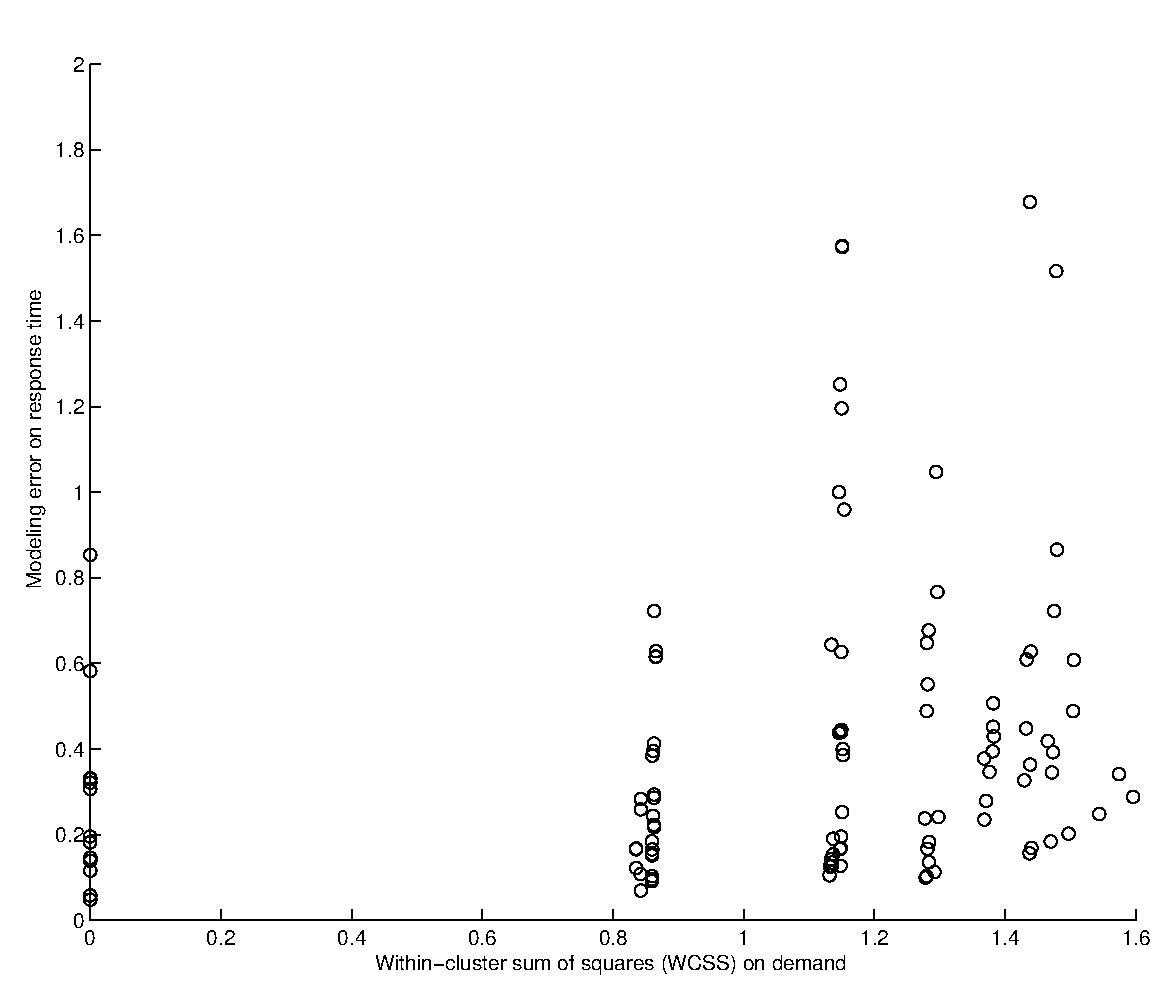
\includegraphics[width=0.7\textwidth]{image/clustering_error_corelation.eps} 
	\caption[The correlation between the within cluster sum-of-squares (WCSS) for demands and the modelling error.]{Correlation between the within cluster sum-of-squares (WCSS) for demands and the modeling error achieved on the response time's estimation.}
	\label{fig:cluster-sum-of-squares}
\end{figure}

\section{Estimation and Clustering for highly variable demands}  
Our TPC-W experiment covered a short interval; so the service demands did not vary a lot. As a result, it was unlikely that a class moved from one cluster to another. However, in the long run (e.g. a month in real system measures), classes might change place due to variation in the CBMG (and consequently service visits and service demands).   

A simulated experiment to investigate the effectiveness of the algorithm under non-uniform variations in demands was performed. This experiment showed the efficiency of the clustering and estimation for a web-based application where the estimated parameters change at different rates and phases. 
 The simulator software used was the CSim discrete event-based simulator. 
To keep the presentation simple but also to highlight the merits of the proposed method, in the simulation, we varied the think time $Z_c$ and the CPU demands, and kept $N_c$ constant.        


% This web-based application is an e-commerce site with 8 URLs (browse, buy, checkout, admin, login, logout, add, and remove). 
The system has 8 classes (c1-c8), two services (s1,s2), and two servers (w,d). Each service has only one replica, and each replica is placed on an individual server. Replicas are referred to as $j1$ and $j2$, or web and database.        
\begin{figure}[htbp]
	\centering
	%width=0.7\textwidth
   \includegraphics[ width=154mm, height=114mm]{image/image11.eps}
%	
\includegraphics[bb=0mm 0mm 208mm 296mm, width=84.8mm, height=68.7mm, viewport=3mm 4mm 205mm 292mm]{image/image12.eps}
	\caption[A sample service demands for 8 different classes on two services.]{Service demands for 8 different classes [c1,c2,c5,c6,c7,c8] on two services.
	}
	\label{fig:service-demands-different-classes}   
\end{figure}
 
 The classes are associated with a number of users ($N_c$), a mean user think time ($Z_c$), and time variant service demands $d_{c,\text{w}}$ and $d_{c,\text{db}}$. The service demands follow a sine curve with the same period, but different phases (see Figure \ref{fig:service-demands-different-classes}). Because of demand variations, classes migrate from one cluster to another, and the clusters evolve over time. In real applications, the service demands are not likely to change that dramatically, and we consider those variations as a stress load on the algorithm. Because of the variation of the service demands, we expect that the different classes will be re-clustered periodically.                                                                     

 Table \ref{tab:changes-clustering-structure} shows the clusters suggested by the K-means algorithm. The acceptable modeling error $A$ is set to 8\% over 421 simulation steps. The column `Action Nature' indicates the kind of change that has occurred when the past and current clusterings are compared. Ag, Br, Re, and Mv stand for aggregation, breaking, re-structuring, and movement respectively. The columns, "grouping (pre-event)" and "grouping (post-event)" represent the shape of the clusters before and after the re-clustering. % Note that in each re-clustering, the clusters are re-computed from scratch.  % ; meaning that the algorithm oblivious to `Action Nature.' 
\begin{table}
	\centering
\begin{tabular}{|p{0.3in}|p{0.8in}|p{2in}|p{2in}|} \hline 
Step & Action\newline Nature & Grouping\newline (Pre-event) & Grouping (Post-event) \\ \hline 
12 & Ag, Mv & [c1,c5,c6,c8] [c2,c7] [c3] [c4] & [c1,c2,c7,c8] [c3,c4]  [c5,c6] \\ \hline 
35 & Br & [c1,c2,c7,c8] [c3,c4] [c5,c6] & [c1,c2,c7,c8] [c3] [c4] [c5,c6] \\ \hline 
147 & Mv & [c1,c2,c7,c8] [c3] [c4] [c5,c6] & [c1,c5,c6,c8] [c2,c7][c3][c4] \\ \hline 
208 & Ag, Mv & [c1,c5,c6,c8] [c2,c7] [c3] [c4] & [c1,c2,c7,c8] [c3,c4] [c5,c6] \\ \hline 
239 & Br & [c1,c2,c7,c8] [c3,c4] [c5,c6] & [c1,c2,c7,c8] [c3] [c4] [c5,c6] \\ \hline 
340 & Mv & [c1,c2,c7,c8] [c3] [c4] [c5,c6] & [c1,c5,c6,c8] [c2,c7][c3][c4] \\ \hline 
400 & Br, Mv & [c1,c5,c6,c8] [c2,c7] [c3] [c4] & [c1,c2,c7] [c5,c6,c8] [c3,c4] \\ \hline 
\end{tabular}
	\caption[Changes in clustering the structure of user classes due to service demand change.]{Changes in clustering the structure of user classes due to service demand change.}
	\label{tab:changes-clustering-structure}  
\end{table}

Figure \ref{fig:tracked-demands}(a) shows the variation of the service demands in a changing cluster ([c2,c7]+[c1,c8]). Real and tracked service demands for the cluster are shown in Figure \ref{fig:tracked-demands}(b) while the modelling error is depicted in Figure \ref{fig:tracked-demands}(c). 
 \begin{figure}
	\centering
	\subfloat[][]{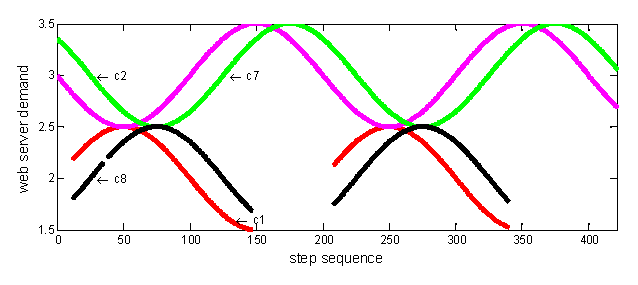
\includegraphics[width=0.6\textwidth]{image/variation-of-service-demands.eps}\label{fig:estimation-sub1}}  \\
	\subfloat[][]{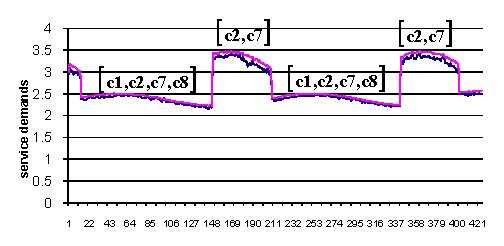
\includegraphics[width=0.6\textwidth]{image/real-and-tracked-service-demands2.eps}\label{fig:estimation-sub2}} \\
	\subfloat[][]{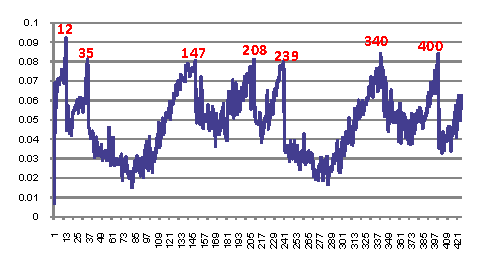
\includegraphics[width=0.6\textwidth]{image/the-modeling-error.eps}\label{fig:estimation-sub3}} \\
	\caption[An estimation case study: service demands, clusters, and modeling error.]
	{Represents (a) the variation of service demands,
		(b) real and tracked service demands for 2 clusters [c2,c7] and [c2,c7,c1,c8], 
		and (c) the modeling error with dynamic clustering applied.  }
	\label{fig:tracked-demands}
\end{figure}

According to Figure \ref{fig:tracked-demands}(a),  at step 50, $(d_{c1,\text{w}},d_{c1,\text{d}})$ and $(d_{c2,\text{w}},d_{c2,\text{d}})$ get close. This suggests that c1 and c2 should be in the same cluster near that step. At step 150, the service demands of c1 and c2 are quite different, indicating that these two classes are more likely in different clusters. These observations are consistent with our results where the clustering at step 50 is [c1,c2,c7,c8][c3][c4][c5,c6] and [c1,c5,c6,c8][c2,c7] [c3][c4] at step 150. Note that c1 and c8 are shown in Figure \ref{fig:tracked-demands}(a) only when they are part of the cluster [c2,c7,...]. This explains the step-function-like behaviour of the estimated demand for the changing cluster in Figure \ref{fig:tracked-demands}(b).

Based on Figure \ref{fig:tracked-demands}(c), during the simulation the modelling error exceeds the threshold A, 7 times. This means the classification algorithm described in Section III.B is activated 7 times among the 421 steps. One can see that not every re-clustering necessarily results into a different number of clusters. For example, at step 147, the clustering changes from [c1,c2,c7,c8][c3][c4][c5,c6] to [c1,c5,c6,c8][c3][c4][c2,c7]. The number of clusters remains the same, but c1 and c8 have been moved to a different cluster. Figure \ref{fig:number-clusters-over-time} shows that the total number of clusters changes only 4 times over the 400 steps.
\begin{figure}[h]
	\centering
	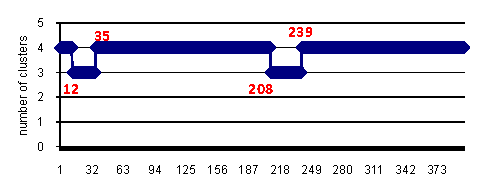
\includegraphics[width=0.7\textwidth]{image/number-clusters-versus-simulation-steps.eps}
	\caption[An estimation cases study: number of clusters over time.]{An estimation cases study: number of clusters over time.}
	\label{fig:number-clusters-over-time}
\end{figure}

We can conclude that our estimation and classification algorithm works quite well, since it is able to keep the error below $A$=0.08 with the smallest number of clusters and acceptable frequency of re-clustering. 

The algorithm also satisfies our claim: being able to exploit the complexity-accuracy trade-off and to keep both the modeling error and the monitoring and computational cost low. In terms of cost, our algorithm yielded half the required clusters (See Figure \ref{fig:number-clusters-over-time}) compared to full classes estimation, which from the theory reduces the estimation cost by a factor $2^3$ ($\frac{1}{2^3}$ of the original cost) and reduces the number of needed measurements by $4J$ (i.e. four fewer metrics for each replica). This is due to the fact that, the cost of the Kalman estimation in each step is dominated by Kalman gain calculation, which is $O(l^3)$ while $l$ is the number of measured variables. The reason is that the dominating term during gain calculation is an inversion of a matrix of size $l\times l$:
\begin{equation}
	K_n=P^-_nH^T_n{(H_nP^-_nH^T_n+\ R_n)}^{-1}
\end{equation} 
In this equation, $R_n$ is measurement noise covariance matrix with size $l\times l$.

In terms of accuracy, it was able to keep the error near zero compared to the case of fully aggregated classes. See Figure \ref{fig:comparison-of-modeling-error} for the error comparison between our algorithm, the one cluster case and the full classes estimation. 
\begin{figure}[h]
	\centering
	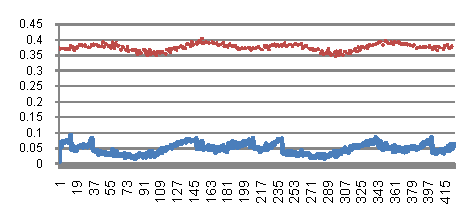
\includegraphics[width=0.7\textwidth]{image/comparison-modeling-error-one-cluster-dynamic.eps}
	\caption[Comparison of the modeling error for one cluster case, dynamic clustering case, and full classes estimation.]{Comparison of the modeling error for one cluster case (dotted line), dynamic clustering case (solid line), and full URLs estimation (solid horizontal line at $y=0$).}
	\label{fig:comparison-of-modeling-error}
\end{figure}

\section{Summary} 
\label{sec:conclusions-and-future-work} 
   Using Kalman filtering and LQM for hidden performance parameters estimation, is a promising approach. However, it introduces lots of monitoring overhead when the number of classes is increased. To mitigate this, we investigated a tracking approach, that identifies the performance parameters of groups of classes (we call them clusters) instead of individual classes. We proposed an algorithm that finds the appropriate number of clusters with a pre-defined clustering accuracy. 

We applied the clustering and tracking algorithm to two scenarios: 
(i) In the first experiment, we used our technique on the TPC-W benchmark deployed on a cluster of web servers. The workload was obtained from the well-known FIFA98 archives. In this experiment, first, we observed that the modelling error is reduced as the number of clusters increases. Second, we tested 140 different random ways to cluster the classes and computed their average error values ($E$). We observed that a clustering with a smaller average distance of classes to centroids (i.e., with smaller cluster sum-of-squares) has less error. Thus, we showed the usefulness of the K-means algorithm. Moreover, we dynamically computed the number of needed clusters that keep the modelling error under a threshold. For example, if one can accept 17\% error, the number of needed clusters for estimation would be dropped from 14 to 9 on average.
(ii) In the second experiment, we deployed our algorithm on a system with 8 classes. It was shown that our Extended Kalman filter could track hidden states successfully, and the correctness of the filter rose as it tried more classes and re-estimated service demands.

Our algorithm also satisfies our claim: being able to exploit the complexity-accuracy trade-off and to keep both the modeling error and the monitoring and computational cost low. 

In terms of cost, our algorithm yielded half the required clusters compared to full classes estimation, which from the theory reduces the estimation cost by a factor $2^3$ ($\frac{1}{2^3}$ of the original cost). 








 



\chapter{Optimal Resource Share Adjustment in Cloud Using Dynamically Tuned Empirical Models} 
\label{ch:optimal_tuning_of_application_resource_shares} 
%\begin{center}
%\textbf{This chapter contains material from Ghanbari et al. \cite{hamoun_ghanbari_feedback-based_2010}}.
%\end{center}

In order to allocate a set of limited resources to a set of applications optimally, there is a need for a model of the application service center. 
A portion of the related work on optimal deployment such as \cite{li_fast_2009,li_performance_2009} assumes that the service center follows an accurate first principle model. They suggest using a filter-based approach such as \cite{zheng-integrated-2011} to estimate the parameters of this model adaptively (i.e. through unsupervised learning).   
However, there is no guarantee that these first principle models accurately represent a service center. It is usually very hard to model all aspects of a service center such as software contention, concurrency, remote calls, a limited amount of memory, and a limited amount of network bandwidth.  

In contrast to the first principle approach, an empirical approach can use a model obtained by regression analysis of application performances. The major problem with present empirical models, is the lack of tuning, based on actual measurement data (e.g. resource utilizations).  
When applications are deployed in a production environment, the models start to lose accuracy. This inaccuracy is mainly because the production conditions are different from the test conditions \footnote{test conditions are used to build the training data sets.}.
 
Our contribution is to increase the accuracy of the empirical models by dynamic tuning using measurement data captured in real-time. We also trace the accuracy increase in the overall performance of the allocation. We investigate if a model built off-line through a nonlinear regression and dynamically tuned through an Extended Kalman Filter, can outperform a model which is not tuned. The other differences between our approach and previous work are in the use of the decomposed models, and in the use of a customized optimization routine to optimize the defined utility functions.   

We show that static non-tuned application models result in a suboptimal allocation decision for some applications leading to missed SLAs. In contrast, we found that the use of dynamically tuned models resulted in more efficient resource allocations, closer achievement of SLAs and better utility. 

The model we develop in this chapter corresponds to a virtualized private data center with limited resources. The unique feature of virtualized data centers when work conservation is enabled is that virtual machines isolate the applications. So, performance of each application can be modelled separately based on allocated resources.
Each application's performance is modelled based on the amount of resources allocated to its VMs. Since the simulator used in this chapter simulates applications with open workloads, we use open queuing network models as a basis of our model.

We assume that the cloud provider only tries to optimize the applications' performances by tuning the amount of resources allocated to the existing fixed set of VMs.  Directly changing ``relative share'' of the allocated resource to each single VM can be done through the hypervisor's scheduler parameters. In addition, the assumption is that the cloud provider can monitor the performance metrics of the applications and thus build models based on the performance metrics and the given resources.
 
Our approach is presented in Figure~\ref{fig:feedback-based-optimization}. 
In this approach, for each application, the cloud provider maintains a dynamically updated performance model. 
A utility function based on a specific service level objective (e.g., response time) is also maintained for each application.    
The performance model for each application is updated periodically based on the measured performance attributes.  The cloud provider then performs a system-wide global optimization (see Section~\ref{sec:optimization-through-subgradient}) using the performance models and determines new resource allocations for each application for the following period. 
\begin{figure}[h]
	\centering
		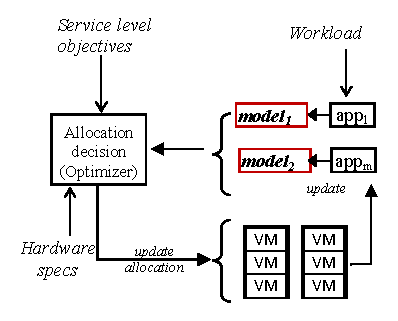
\includegraphics[width=0.45\textwidth]{image/centralized1/image2new}
	\caption[Architecture of the proposed feedback-based optimization approach for private cloud.]{Feedback based optimization of resource shares.} 
	\label{fig:feedback-based-optimization}
\end{figure}

\section{General Definitions} 
\label{sec:general-defs}
In this section, we define the necessary notation used in the specification of the problem. 

\textbf{Applications:} 
To denote applications we use the symbol $c$ since one way to model applications is through classes as defined in a queuing model. Consider applications \texttt{$c_1$},\ldots, \texttt{$c_C$}. Each application runs within one or more VMs and experiences a particular workload.  
For modeling purposes in this chapter, we assume each application experiences an open workload with certain inter-arrival time(s) denoted by $\tau_c$. 
Also, we assume $d_c$ is application $c$'s hardware demand per application request (i.e. the number of CPU cycles for each request to be processed).

\textbf{Hardware Structure:} We assume a private service centre with heterogeneous resources composed of $H$ hosts or physical machines (PM)s represented by the set ${h_0,...,h_H}$. We also assume each host has one resource type. The capacity of the resource of host $h$, is denoted by $\capp_{h}$.   

\textbf{Utility Function:} 
Figure~\ref{fig:service-level-utility-functions} represents a sample service level utility function, where the vertical line indicates the SLA target for the application and utility decreases as the value of the response time approaches the SLA limit.
It is worth noting that any decreasing differentiable quasi-convex function can also be used as a service level utility function, and the only feature of this function is simplicity of the presentation in mathematical form.
The shape of the function, especially after passing the SLA threshold, will affect the behaviour of the optimization algorithm. 
\begin{figure}[h]
	\centering
	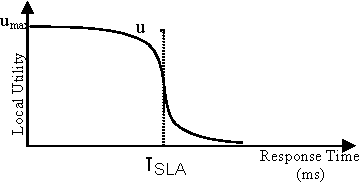
\includegraphics[width=0.45\textwidth]{image/centralized1/image3new}
	\caption[A smooth service level utility function used in a feedback-based optimizer in the private cloud.]{A smooth service level utility function; the vertical line indicates the service level objective of the application (as defined in the SLA).}
	\label{fig:service-level-utility-functions}
\end{figure}

\textbf{Placement:} 
 We consider the VMs of applications which are already deployed on physical machines.
 We specify this deployment through a matrix $\xi$. For each application $c$ and host $h$, if there is a VM allocated to the application on the host, the element $(c,h)$ of matrix $\xi$ is 1 and otherwise  it is 0. 

\textbf{Resource Shares:}
 We represent the allocation of VMs on PMs by a $C \times H$ matrix $\mu^\theta$. Each element $\mu^\theta_{c,h}$ of $\mu^\theta$ denotes a resource allocation defining the percentage of the total resource (i.e. CPU) capacity of the PM $h$ allocated to a running VM of application $c$.  

\section{Problem Formulation}  
\label{sec:contribution2-problem-formulation} 
 Our objective is to maximize a global utility function (sum of application-provided resource-level utility functions $u_c$), subject to a set of capacity constraints which come from the physical layer of the private cloud. 
The optimization problem addressed here can be expressed as follows:
\begin{equation} \label{eq:opt-def}
\begin{split}
\text{given:} 
& \xi_{c,h} \forall c\forall h,
 \tau_c \forall c,l_{\capp,\speedFactor},
 d_{c} \forall c\\
\underset{\mu^\theta}{\text{maximize}} & \sum_{c=0}^{C} u_c(R_c)   \\
\text{subject to: } 
& \sum_{c=0}^{C}{\mu^\theta_{c,h}}<\capp_h \ & \forall h  \\
&  \mu^\theta_{c,h} \geq 0 & \forall h\forall c \\
& R_c=l_{\capp,\speedFactor}(\boldsymbol\mu^\theta_{c},\tau_c,d_{c}) & \forall c \\
& \mu^\theta_{c,h}.\xi_{c,h}=\mu^\theta_{c,h} & \forall c \forall h
\end{split}
\end{equation}
where 
$d_c$ is application $c$'s hardware demand per request and $d_{c}$'s units is the number of CPU cycles.
 
$l$ is a model that maps the application $c$'s resource allocations (i.e. $\boldsymbol\mu^\theta_{c}$) to the service level measure (i.e. response time) of the application, $u_c$ is the local utility function for the application $c$, $\mu^\theta_{c,h}$ represents the allocation of a physical machine $h$ to application $c$. 
In a case study we use a simulator that includes the number of CPU cycles as an input parameter. Each $\mu^\theta_{c,h}$ will be considered to have the unit of million instruction per-second (MIPS). $\boldsymbol\mu^\theta_{c}$ represents the vector of resources allocated to an application $c$ on different hosts. 
The equality constraint $\mu^\theta_{c,h}.\xi_{c,h}=\mu^\theta_{c,h} \  \forall c \forall h$ implies that the only elements of $\mu^\theta_{c,h}$ that need to be optimized are those whose corresponding element in $\xi$ is 1. Other elements of $\theta$ will be considered 0. It is an implication of the first and second inequality constraints that each allocation $\mu^\theta_{c,h}$ is constrained to lie in the interval $[0,\capp_h]$ meaning that an application can maximally get the whole capacity of a PM. The equality constraint relates the response time of each application to the workload intensity, hardware demands, and the given capacities.

Note that the proposed problem solution has a best effort nature, and we treat a service level objective (i.e. target on a specific QoS metric) as a soft constraint by incorporating it into the objective function. 

\section{Selecting an Empirical Model}
A performance model can be used to relate the physical layer specification of a customer's application (e.g. it's given resource shares) and its associated workload to a service level measure (e.g. response time) quantitatively.    
We assume that the response time of each application $c$, can be modelled by the given resources (to VM's) of application $c$ (i.e.$\boldsymbol\mu^\theta_{c}=\{\mu^\theta_{c,1},\dots ,\mu^\theta_{c,H}\}$), the demand of application on the resource types (i.e. here only CPU $d_c$) and the workload of the applications (i.e. $\tau_c$) using the function $l$:
\begin{equation} \label{eq:perf-model_general}
\begin{split}
	%s_c= g(a_{1j},a_{2j},\dots ,a_{nj},{\tau }_c,d_c) \\
	R_c=l_{\capp,\speedFactor}(\boldsymbol\mu^\theta_{c} ,\tau_c,d_{c}) 
	\end{split}
\end{equation} 
 where $\boldsymbol\mu^\theta_{c}$ is a vector of elements $\mu^\theta_{c,h}$, which represent the number of allocated CPU cycles (i.e., measured in MIPS), ${\tau }_c$ denotes the request inter-arrival time in seconds associated with the workload of the application $c$, $d_c$ is application $c$'s hardware demand per request (i.e. the number of CPU cycles for each request to be processed), and $R_c$ is the average response time of the application.

 The nonlinear model is further simplified by using the aggregate resource capacity measure $ \mu^{\theta,\text{Agg}}_c = \sum_{h=1...H}{\mu^\theta_{c,h}}$ instead of the vector of individual values
($\mu^\theta_{c,1},\mu^\theta_{c,2},\dots ,\mu^\theta_{c,H}$):% and replacing $g$
%with $f$:
%\begin{equation} \label{eq:aggregate-cap}
 %\begin{split}
  %s_c= f(\mu^{\theta,\text{Agg}}_c,{\Tau }_c,d_c) \\
  %\text{where}\  \mu^{\theta,\text{Agg}}_c = \sum_{i=1...n}{a_{ij}}       
 %\end{split}
%\end{equation}
  We will assume that all applications deployed on the infrastructure adhere to the same performance model, differing only in the setting
  of various configurable parameters. 
	
	Focusing only on one application called $c$, let $\boldsymbol\beta_{c,t}$ be a vector representing the model coefficients
 and $\left[\mu^{\theta,\text{Agg}}_{c,t},\tau_{c,t},d_{c,t}\right]$ be the measured inputs of the system (i.e. capacities, inter-arrival time and demand) 
at step $t$.  
The model maps $\left[\mu^{\theta,\text{Agg}}_{c,t},\tau_{c,t},d_{c,t}\right]$ and $\boldsymbol\beta_{c,t}$ to the modelled output $R_{c,t}$:
\begin{equation}\label{eq:kalman-model} 
R_{c,t}=f(\left[\mu^{\theta,\text{Agg}}_{c,t},\tau_{c,t},d_{c,t}\right],\boldsymbol\beta_{c,t})
\end{equation}
where $f$ is a runtime approximation of the service level function (or performance model) $l$ defined earlier.

While the function $f$ can take several forms, the online-estimation techniques and optimization method are general and will be considered next in Subsection~\ref{sec:online-model-estimation} and Section~\ref{sec:optimization-through-subgradient}.
% -----------------------------------------------


We considered three parametric forms for function $f$: 
\begin{enumerate}
\item A simple linear model only containing predictor variables\footnote{The model is linear in the parameters $\beta_{c,i}$ not predictor variables.}:\\
$f(\left[\mu^{\theta,\text{Agg}}_{c},\tau_{c},d_{c}\right],\boldsymbol\beta_{c}) = \beta_{c,1} +  \beta_{c,2} d_c - \beta_{c,3} {\tau}_c - \beta_{c,4} \mu^{\theta,\text{Agg}}_c$
\item A more complex linear model with interaction terms \footnote{The interaction term is the product of the subset of our original predictors.} $\mu^{\theta,\text{Agg}}_c \tau_c$ and $\mu^{\theta,\text{Agg}}_c d_c$ to capture the effect of $\mu^{\theta,\text{Agg}}_c$ on response time at different inter-arrival times and demands:\\
$f(\left[\mu^{\theta,\text{Agg}}_{c},\tau_{c},d_{c}\right],\boldsymbol\beta_{c}) = \beta_{c,1} + \beta_{c,2} d_c-\beta_{c,3} {\tau}_c-\beta_{c,4} \mu^{\theta,\text{Agg}}_c-\beta_{c,5} \mu^{\theta,\text{Agg}}_c d_c + \beta_{c,6} \mu^{\theta,\text{Agg}}_c {\tau}_c$
\item  A non-linear model derived from the mean value based formula for open queuing networks ($R=D/(1-\lambda D)$) \cite{lazowska_quantitative_1984} extended to account for capacity:\\
$f(\left[\mu^{\theta,\text{Agg}}_{c},\tau_{c},d_{c}\right],\boldsymbol\beta_{c})=\frac{\beta_{c,1} d_c}{\mu^{\theta,\text{Agg}}_c-\beta_{c,2} d_c/{\tau}_c}$ 
\footnote{This equation can be derived by substituting $D_c$ with
  $d_c/\mu^{\theta,\text{Agg}}_c$ and ${\tau}_c$ with $1/{\tau}_c$ from the base formula, and adding model coefficients (i.e. $\beta_{c,1}$ and
  $\beta_{c,2}$) to compensate for the differences between the system and a pure queuing model. The substitution requires the inter-arrival time
  ($\tau $) to be a homogeneous Poisson process, and inter-arrival
  times ($\tau $) to be exponentially distributed with parameter
  $\tau $ (mean 1/$\tau $).}
\end{enumerate}

To investigate the accuracy of the models, a data-set of the sample application's performance was generated synthetically by invoking the CloudSim simulator \cite{CLOUDSIM2010} using random values for the capacity, demand and the inter-arrival time. Figure~\ref{fig:arrival-rate-effect-on-response-time} presents a partial visualization of the data-set. 
\begin{figure}
	\centering
	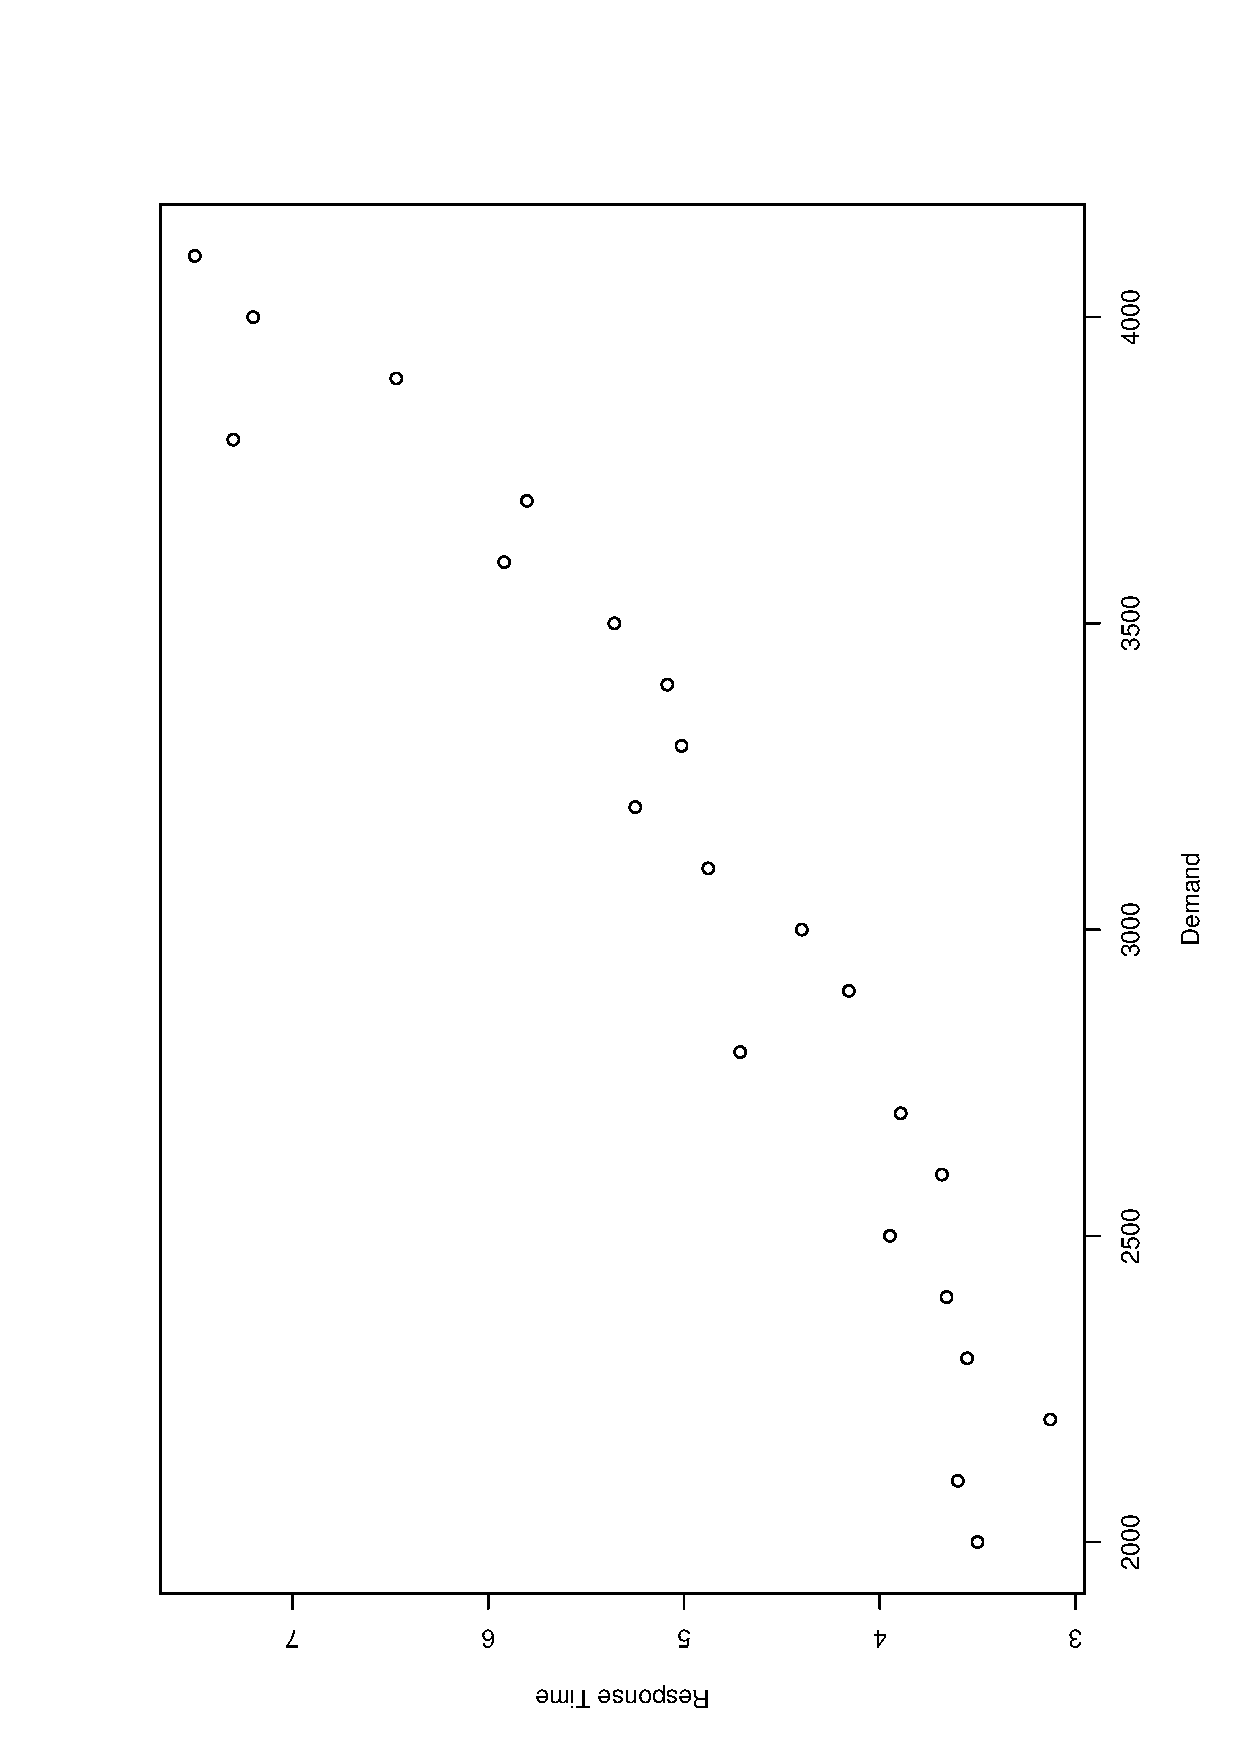
\includegraphics[width=0.45\textwidth,angle=-90,origin=c]{image/centralized1/demand_response_time} \\
	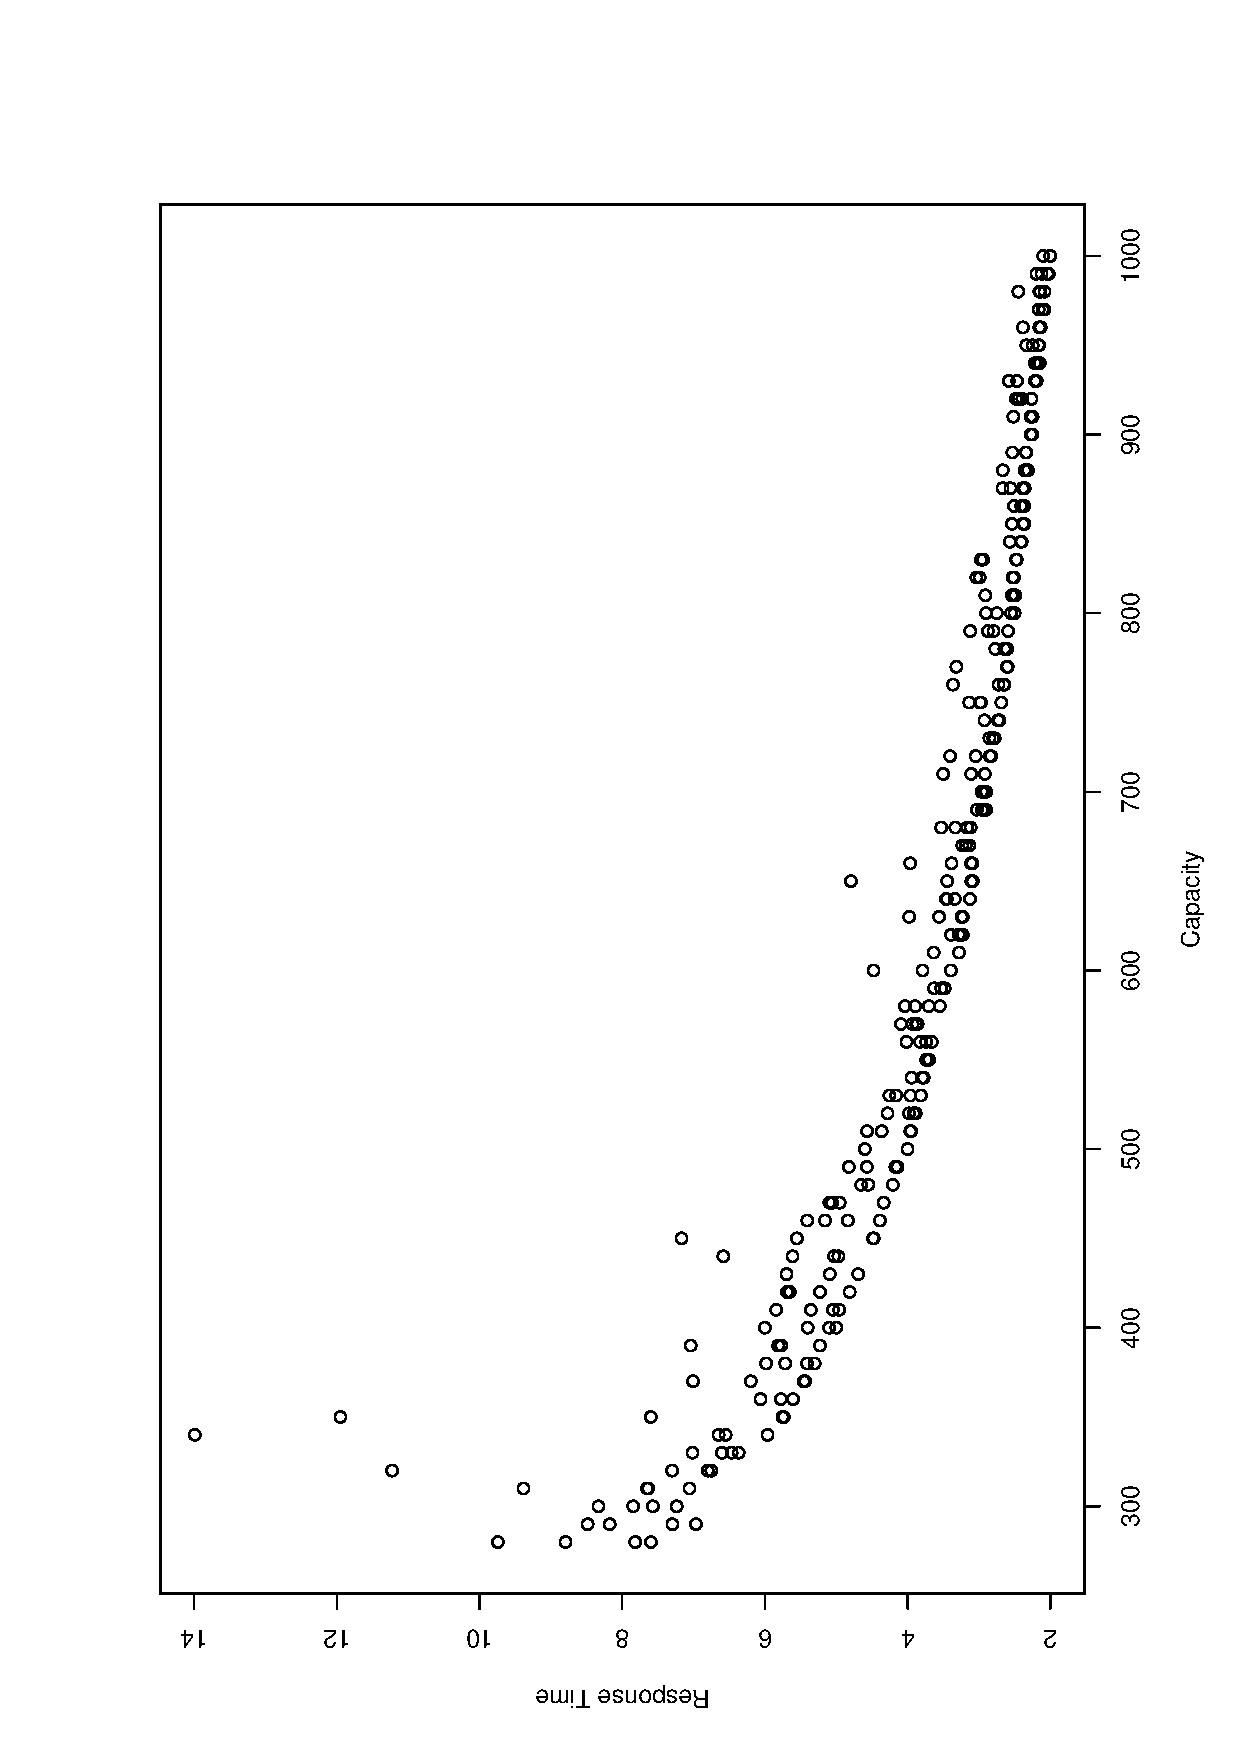
\includegraphics[width=0.45\textwidth,angle=-90,origin=c]{image/centralized1/response_time_capacity}
	\caption[Visualization of pairwise relation between input parameters (capacity,demand) and the response attribute (i.e. response time) for a simulated application.]{Visualization of pairwise relation between input parameters (capacity,demand) and the response attribute (i.e. response time) for a simulated application running on a single VM.}
	\label{fig:arrival-rate-effect-on-response-time}
\end{figure}
A regression analysis was then performed on the resultant data for each model, allowing confidence intervals to be computed for all model parameters.
Usually, the use of a predictor variable is meaningful if its estimated coefficient's confidence interval is far from zero\footnote{There is no proven way for finding if the interval is far enough from 0.}. Moreover, a wide confidence interval usually means lack of accuracy and the need for more data. We formed approximate 95\% confidence intervals for each $\beta_{c,i}$ using mean, standard error, and the normality assumption, to indicate the accuracy and significance of each $\beta_{c,i}$. 
The approximate 95\% confidence intervals for coefficients were quite narrow, and the margins of error were orders of magnitude smaller than the coefficient. This result implies that the amount of data for modeling was adequate.
However, when applying the regression analysis using the linear models, the intervals were very near to zero and coefficients were not significant.
One possible explanation for the lack of significance is that only the fixed portion of the response time (i.e. delay at server) was accounted for in linear models, not the queuing delay which might grow exponentially. 
 The estimated coefficients for the nonlinear model were relatively significant.
As the result of this analysis, the non-linear model's use was validated. 



%\section{Estimation: Online versus Off-line}   
%\label{sec:Modeling-response-time}

% 
\subsection{Online Estimation}
\label{sec:online-model-estimation}

Let $z_{c,t}$ be the measured system output (e.g. response time) at step $t$. 
We further assume that $\beta_{c,t}$ changes according to a random walk:
\begin{equation}
	\boldsymbol\beta_{c,t+1}=\boldsymbol\beta_{c,t}+w_{c,t} \\
\end{equation}
where $w_{c,t}$ represents some Gaussian noise.
A filter maintains the estimate of $\boldsymbol\beta_{c,t}$ and updates it using the linear feedback equation based on new measurements $\left[\mu^{\theta,\text{Agg}}_{c,t},\tau_{c,t},d_{c,t}\right]$ and $z_{c,t}$: 
\begin{equation}\label{eq:kalman-update} 
	\boldsymbol\beta_{c,t} = \boldsymbol\beta_{c,t-1}+ K_{c,t}(z_{c,t} - R_{c,t})
\end{equation}
where $t$ denotes a discrete time index, $K_{c,t}$, the dynamically computed
``Kalman Gain'' matrix and $z_{c,t}-R_{c,t}$ denotes the prediction error\footnote{Note that $R_{c,t}$ was calculated using equation~\ref{eq:kalman-model}.}. With assumptions of system linearity and Gaussian noise, the calculated Kalman gain $K_{c,t}$, is guaranteed to minimize the 
estimation errors for $\boldsymbol\beta_{c,t}$. The updated state will result in a dynamic
model $f(\left[\mu^{\theta,\text{Agg}}_{c,t},\tau_{c,t},d_{c,t}\right],\boldsymbol\beta_{c,t})$ that will be accessed multiple times during optimization cycles. 
Function $f$ and its non-measurable and measurable parameters can have many representations (as shown in Section \ref{sec:case-studies}). 

\section{Optimization}
\label{sec:optimization-through-subgradient}
In this section, the utility maximization problem defined in equation~\ref{eq:opt-def} is solved. Algorithm~\ref{algorithm1} represents a centralized solution for this problem using the primal method.  

The input to the algorithm includes the initial capacities (i.e., $\mu^\theta_0$), the number of iterations during optimization ($k_{\text{max}}$), the performance model ($f_{\boldsymbol\beta_{c,t}}$) and the utility model $u_c$ for each application. 
The output of the algorithm is the optimal allocation matrix ($\mu^\theta_{\text{opt}}$), and maximum utility gained from that allocation ($fp_{best}$) that is obtained iteratively using $k_{\text{max}}$ iterations. )
 \begin{figure} 
\begin{algorithm}[H]  
	\small
	\SetAlgoVlined
	\SetKwInOut{Input}{input}
	\SetKwInOut{Output}{output}
	\SetKwInOut{Initialize}{initialize}
  \SetAlFnt{\tiny}
\footnotesize\Input{
initial capacities $\mu^\theta_0$, 
maximum number of iterations $k_{\text{max}}$, 
performance model $f$,  
utility model $u_c$ forall $c$,
model coefficients $\boldsymbol\beta_{c,t}$ for all $c$}
\Output{optimal allocation $\mu^\theta_{\text{opt}}$, Maximum utility $fp_{\text{best}}$}

initialize: $fp=-\infty$, $fp_{best} =-\infty$, $\mu^\theta=\mu^\theta_0$, $k=0$

\While { $k < k_{\text{max}}$}
{
	compute constraint value $U_i$ for each PM:
	\nllabel{al1-step_1} 
	$U_i(\mu^\theta)=\left(\sum_{c=0}^{C}{\mu^\theta_{c,h}}\right)-\capp_h $

	\If {\text{no constraint is violated:} $max(U_i(\mu^\theta))>0$ //move towards optimum:}
	{
		compute global utility function:
		%using equation~\ref{eq:opt-def}.
		\nllabel{al1-step_2.1} 
		%$U_0 = \sum_{c=0}^{C}  u_c(l_{\capp,\speedFactor}(\boldsymbol\mu^\theta_{c},\tau_c,d_{c})) $
		$U_0 = \sum_{c=0}^{C}  u_c(f(\left[\mu^{\theta,\text{Agg}}_{c,t},\tau_{c,t},d_{c,t}\right],\boldsymbol\beta_{c,t})) $

		record the global maxima: % using equation~\ref{eq-record-global-maxima}.
		\nllabel{al1-step_2.2} 	
		$fp_{\text{best}} \gets max(U_0(\mu^\theta), fp_{\text{best}})$ 

		calculate objective function's subgradient:% using equation~\ref{eq-calculate-objective-subgradient}.
		\nllabel{al1-step_2.3} 
			$g=\partial U_0(\mu^\theta) / \partial \mu^\theta $

		move towards subgradient and the optimum: % using equation:%~\ref{eq-moving-towards-objective-function}.
		\nllabel{al1-step_2.4}			
		$  \mu^\theta \gets \mu^\theta + \alpha g_0$
	}
	\ElseIf{there is some violated constraint}{

	  find most violated constraint using equation:%~\ref{eq-find-most-violated-constraint}.
		\nllabel{al1-step_3.1}
		$m \gets argmax_i(\|U_i(\mu^\theta)\|)$ 
	  \BlankLine

		compute the subgradient value of most violated  constraint as follows:% using equation:%~\ref{eq-calc-subgr-of-most-violated-constraint}.
		\nllabel{al1-step_3.2} 
		% $[(k=m \wedge placement(k,c)=1) \rightarrow (g_m)_{k,c} = 1  ] \wedge   [k \neq m  \rightarrow (g_i)_{k,c} = 0  ]  \  \forall k \forall j$ 
		
		\ \ for each $c$, if $\xi_{m,c}=1$ then  $g_{m,c}\gets 1$ else $g_{m,c}\gets 0$ \nllabel{al1-step_3.2.1}% $\forall c$
		
		\  \ for each $h$ and $c$, if $h \neq m$ then $g_{h,c}\gets 0$   \nllabel{al1-step_3.2.2}%\forall h \forall c$ 
		\BlankLine

		select step size:%based on equation~\ref{eq-step-size-select}.
		\nllabel{al1-step_3.3}
		$\alpha  = (U_i(\mu^\theta_{c,h}) + \epsilon)/(\|g\|^2_2)  $
		\BlankLine

		move away from subgradient and the optimum:
		using equation~\ref{eg:project-subgradient}.\nllabel{al1-step_3.4}
		$\mu^\theta \gets \mu^\theta - \alpha g_i$ 
		\BlankLine
	}
	project each individual variable based on its local constraint:%
	%using equation~\ref{eq-check-local-bound}.
	\nllabel{al1-step_4}  		
	$ \mu^\theta_{c,h} = min(max(\mu^\theta_{c,h},0), \capp_h ) \ \forall h \forall j $ 
	\BlankLine

	$k = k + 1$\; 	
	\BlankLine      
}
$\mu^\theta_{\text{opt}} = \mu^\theta_{c,h}$\;
\caption[A centralized solution for the feedback-based optimization problem using the primal method.]{A centralized solution for the problem using primal method.  
% The equations referred to are presented in Table~\ref{tab:equations}.
}
\normalsize
\label{algorithm1}
\end{algorithm}
\end{figure}

%------------------------------------------
%~\thetb #1
\newcounter{tb}
\newenvironment{tb}[1][]{\refstepcounter{tb}}

\begin{tb}\label{eq-compute-PM-constraint}\end{tb} 
\begin{tb}\label{eq-compute-global-utililty-function}\end{tb}  
\begin{tb}\label{eq-record-global-maxima}\end{tb} 
\begin{tb}\label{eq-calculate-objective-subgradient}\end{tb} 
\begin{tb}\label{eq-moving-towards-objective-function}\end{tb} 
\begin{tb}\label{eg:project-subgradient}\end{tb} 
\begin{tb}\label{eq-find-most-violated-constraint}\end{tb} 
\begin{tb}\label{eq-calc-subgr-of-most-violated-constraint}\end{tb} 
\begin{tb}\label{eq-step-size-select}\end{tb} 
\begin{tb}\label{eq-check-local-bound}\end{tb} 
  % -----------------------------------
 The algorithm performs $k_{\text{max}}$ iterations. In each iteration it does the
  following:

\begin{enumerate}

\item  Computes the constraint values (a constraint is violated if its value is less than 0). A constraint for each physical machine (PM) is the sum of all resources given to VMs deployed on that PM minus the PM's total capacity (step 1).
\item  If the current allocation point is feasible (i.e. no constraint is violated) the algorithm re-calculates the objective function value $U_0$ using the current allocation ($\mu^{\theta,\text{Agg}}$), performance model $f$ from equation~\ref{eq:perf-model_general}, and utility model $u_j$ defined by the administrator (step \ref{al1-step_2.1} ). 
\item If the objective value was greater than the currently reached maxima, it would be recorded (step \ref{al1-step_2.2}).
\item Then the algorithm calculates the objective subgradient using numerical differentiation (i.e. solving the current performance model multiple times for near values of the current point) as if the problem were unconstrained (step \ref{al1-step_2.3}).
\item Finally, a new allocation matrix is calculated, by moving towards the objective function subgradient with a fixed step size (optimality update, step \ref{al1-step_2.4}).
\item If the current allocation point is infeasible the algorithm chooses the most violated constraint\footnote{Actually, this can be any violated constraint.} (step \ref{al1-step_3.1}).
\item Then the algorithm projects the current point onto the set (half-space) of points that satisfy that inequality constraint. 
 Projection is done by moving towards the opposite direction of the constraint function subgradient, $g_i$ (step \ref{al1-step_3.4}).
% while the subgradiet $g_i$ of a constraint $i$ is defined as follows (see step \ref{al1-step_3.2}): 
%\begin{equation}\label{eq:calc-subgr-of-most-violated-constraint}
%\begin{split}
%g_{ij}=(\partial U_i(a)/(\partial a_{ij}))_{ij} = \\
%\left\{ 
			%\begin{array}{cc}
				%0 & placement(i,j)\neq i \\ 
				%1 & placement(i,j)=i 
			%\end{array}
		%\right.
%\end{split}
%\end{equation}
 The sub-steps \ref{al1-step_3.2.1} and \ref{al1-step_3.2.2} assert that, since each constraint is sum of allocated capacity for each VM, $\partial U_i(x)/\partial x$ is a matrix with same dimensions as $x$ (with 1 in each element that affects the constraint). For example if $f(x)_i=x_1-6$ then $\partial f(x)_i/\partial [x1,x2]=[1,0]$. 
% \footnote{$U_i(a)$  changes proportionally with respect to the capacity change $a_{ij}$ of application $j$ 
%(i.e.  ${(\partial U_i(a)/\partial a_{ij})}_{ij}=1$  only if VM of app $j$ is placed on $PM_i$ ). 
%If a VM of application $j$ is not placed on $PM_i$ , $U_i(a)$ will not change with respect to change of
% $a_{ij}$ and thus  ${(\partial U_i(a)/\partial a_{ij})}_{ij}=0$ .}. 

\item The step size is calculated in step \ref{al1-step_3.3}. While $\epsilon>0$ is a tolerance which can take-on different values (e.g. $10^{-3}$,$10^{-2}$, etc.). 

\item  Finally we check that each allocated capacity is feasible and longer than the local bounds (step \ref{al1-step_4}):
where $lb$ is the lower bound and $ub$ is the upper bounds.

\end{enumerate}


%----------------------------------

 For clarity, the equations referenced by the algorithm are listed in Table~\ref{tab:equations}. 
\begin{table*}[h]
\begin{tabular*}{1.0\textwidth}{p{.02\textwidth}>{$\displaystyle}p{.86\textwidth}<{$} }
 %\toprule
  % \footnotesize \text{Num- } & \text{Equation}  \\
\toprule
1 &  U_i(A)=\left(\sum_{c=0}^{C}{\mu^\theta_{c,h}}\right)-\capp_h \\
2 & U_0 = \sum_{c=0}^{C}  u_c( f(\left[\mu^{\theta,\text{Agg}}_{c,t},\tau_{c,t},d_{c,t}\right],\boldsymbol\beta_{c,t}))  \\
3 & fp_{\text{best}} \gets max(U_0(\mu^\theta), fp_{\text{best}}) \\
4 & g=\partial U_0(\mu^\theta) / \partial \mu^\theta \\
5 &  \mu^\theta \gets \mu^\theta + \alpha g_0 \\
6 & \mu^\theta \gets \mu^\theta - \alpha g_i \\
7 & i \gets argmax_i(\|U_i(\mu^\theta)\|) \\
8 &  [(k=i \wedge \xi_{k,c}=1) \rightarrow (g_i)_{k,c} = 1  ] \wedge   [k \neq i  \rightarrow (g_i)_{k,c} = 0  ]  \  \forall k \forall j  \\
9 & \alpha  = (U_i(A) + \epsilon)/(\|g\|^2_2)  \\
10 & \mu^\theta_{c,h} = min(max(\mu^\theta_{c,h},0), \capp_h ) \ \forall h \forall c \\
\bottomrule
\end{tabular*}
\caption{Equations referenced by Algorithm~\ref{algorithm1}.}
\label{tab:equations}
\end{table*} 
To describe the equations briefly: 
Equation 1 states that the value of the constraint\footnote{Value of a constraint here refers to the degree that the constraint is satisfied (positive values) or violated (negative values).} for each $PM_i$ ($i>0$) is the sum of all resources given to VMs deployed on that PM minus the PM's total capacity.
Equation 2 gives the global utility function $U_0$.
Formula 3 is the incremental recording of objective value.
Equation 4 is used to calculate the objective subgradient as if the problem were unconstrained.
Equation 5 indicates moving towards the objective function subgradient with a fixed step size (i.e. optimality update).
Equation 6 is projecting the current point onto the set of points that satisfy the inequality constraint $i$.
Equation 7 denotes choosing the most violated constraint. 
Equation 8 is calculating the subgradient $g_i$ of a constraint $i$ (i.e. $\partial U_i(\mu^\theta)/\partial \mu^\theta$) while $i>0$. 
Equation 9 calculates the step size in the feasibility update, while $\epsilon>0$ is a tolerance and set to $10^{-3}$. 
Equation 10 checks that each allocated capacity is feasible and is between the local bounds. 

To illustrate the optimization algorithm, we consider a pre-built model of one physical machine hosting two applications, each running on a single VM. Both applications have CPU demands of 5100 and 4100 MIPS per request respectively, and response time thresholds of 16 and 7 respectively. The request inter-arrival time of both applications is 22 seconds, and their $u_{\text{max}}$ is 10.  A single PM's CPU, which is used to host these applications, has a total capacity of 1200 MIPS.
 Assumed capacities $\mu^\theta_{11}$ and $\mu^\theta_{21}$ are the CPU allocation for VM1 and VM2. Figure~\ref{fig:sample-config-space-for-subgradient-optimization} shows the entire configuration space over these capacity allocations, constrained by inequalities:
 $\mu^\theta_{11}+\mu^\theta_{21}<1200$, $\mu^\theta_{11}>280$, and $\mu^\theta_{21}>280$.
Note how the optimizer climbs up the global utility function, hits the constraint (i.e., $\mu^\theta_{11}+\mu^\theta_{21}<1200$) then continues to climb and reach the maximum.

\begin{figure}[h]
	\centering
		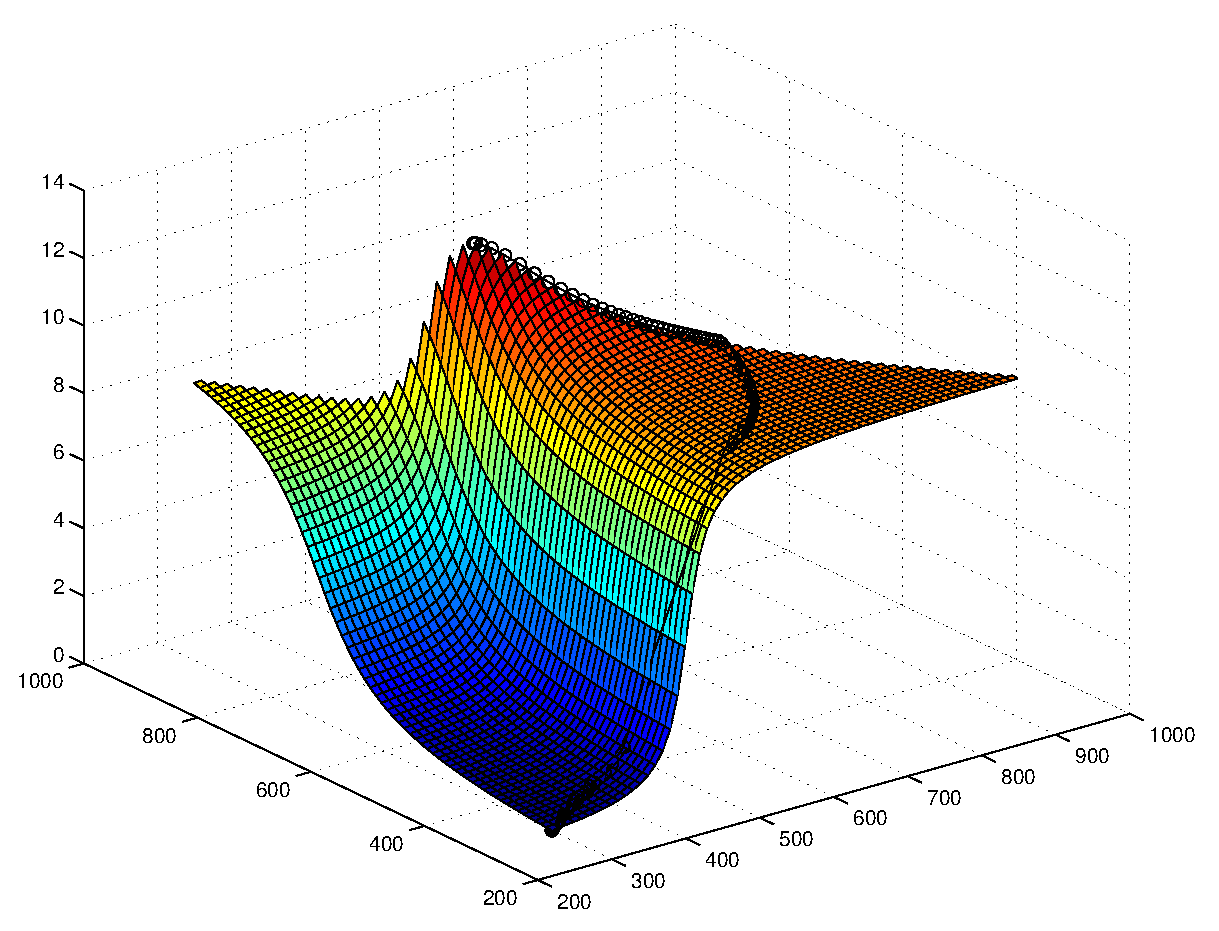
\includegraphics[width=0.8\textwidth]{image/centralized1/twoVM_1PM_optimality}
		\caption{One sample run of subgradient optimization algorithm, finding the
		maximum utility using variations in capacity.}   
	\label{fig:sample-config-space-for-subgradient-optimization}
\end{figure} 


\section{Case Studies}
\label{sec:case-studies}
For the case studies, we simulated a private cloud with the CloudSim~\cite{CLOUDSIM2010} simulator. 
We further considered a very simple local utility function for applications:
\begin{equation} \label{eq:local-utility-formula}
u_c = u_{{\text{max}}_c}\cdot\frac{\left(\arctan(r_{\text{thr}_c}-r_c)+ \pi/2\right)}{\pi} 
\end{equation}
where $u_{{\text{max}}_c}$ denotes the maximum possible utility, $r_{\text{thr}_c}$ denotes the SLA limit (in terms of the minimum response time) and
$r_c$ denotes the actual response time.

\subsection{Case Study One}
\label{sec:case-study-test-simple-deploy}
 % In this section, we study a simulated example to illustrate the applicability of the proposed approach. 
Consider a small cloud configuration with three applications (\texttt{app1}, \texttt{app2}, \texttt{app3}) deployed on two PMs with the following placement matrix:
\[ \xi^T= 
  \left( \begin{array}{ccc}
  1 & 1 & 0 \\
  0 & 1 & 1 \\
\end{array} \right)\] 
That is, \texttt{app1} is deployed on PM1, \texttt{app3} is deployed on PM2, and \texttt{app2} uses both PMs by having a VM on each.

Both of the PMs have single core CPUs with each core having the processing speed of 1200 MIPS and 2 GB of ram. The VMs for applications are identical, each with image size of 1 GB, ram of 512 MB, and bandwidth of 1 GB.

The CPU resource share for each VM is initialized to 280 MIPS but will be adjusted by the optimizer. The applications have workloads with mean CPU demand per request of 4100, 5700 and 500 MIPS respectively. For \texttt{app2}, the load is distributed evenly between the two VMs. We chose the arrival-rates of applications, from the FIFA '98 workload~\cite{arlitt_workload_2000}. The inter-arrival times of requests for all dynamic pages were extracted, on a per-minute basis, from the first six hours of day 21 of FIFA98 workload. To incorporate the time-of-a-day effect, we divided the workload into three 2-hour periods and applied each as an application workload (see Figure \ref{fig:7}). Moreover, we multiplied inter-arrival times of applications by 14, 11 and 8 respectively.
The third application is more transactional in nature (i.e. lower demand and higher inter-arrival time) while the first two are characterized as batch-like.

The utility functions are defined for each application based on equation~\ref{eq:local-utility-formula} with the following parameters for each application:
\begin{align*} \textbf{R}^\text{SLA} = & [15,16,2] \\
 \textbf{u}_{\text{max}} = & [20,10,5]      \end{align*}

For each of 120 samples of inter-arrival times, we submit 20 transactions for each application in the simulator. 
We ran the experiment twice. One run used the static model with the coefficients computed off line as mentioned above.  The second run used the same model but tuned at runtime.
In the case of the tuned model, the new measurements obtained from the simulator (e.g. response times) were used to update the dynamic model's coefficients.  In the case of a static model, the optimizer used the model obtained through regression analysis as-is and no tuning was performed. The optimizer then recalculated the new resource allocations, passed the new allocation vector to actuators to apply it to the system. 

Figure~\ref{fig:case-study1} presents the results. The use of static non-tuned models by the
applications results in a bad allocation decision for \texttt{app2} and leads to failure in meeting app2's SLA (see Figure~\ref{fig:3}).
This results in achieving a suboptimal utility (see Figure\ref{fig:1}).  
In contrast, using dynamic models results in more efficient resource allocations being made, better commitment to SLAs for \texttt{app2} (see Figure~\ref{fig:4}) and better utility (Figure\ref{fig:2}). Figure \ref{fig:5} and \ref{fig:6} represent the allocated capacity to applications over time in case of dynamic models; \ref{fig:5} is for PM1 and \ref{fig:6} is for PM2.     
 
\begin{figure}
	\centering
 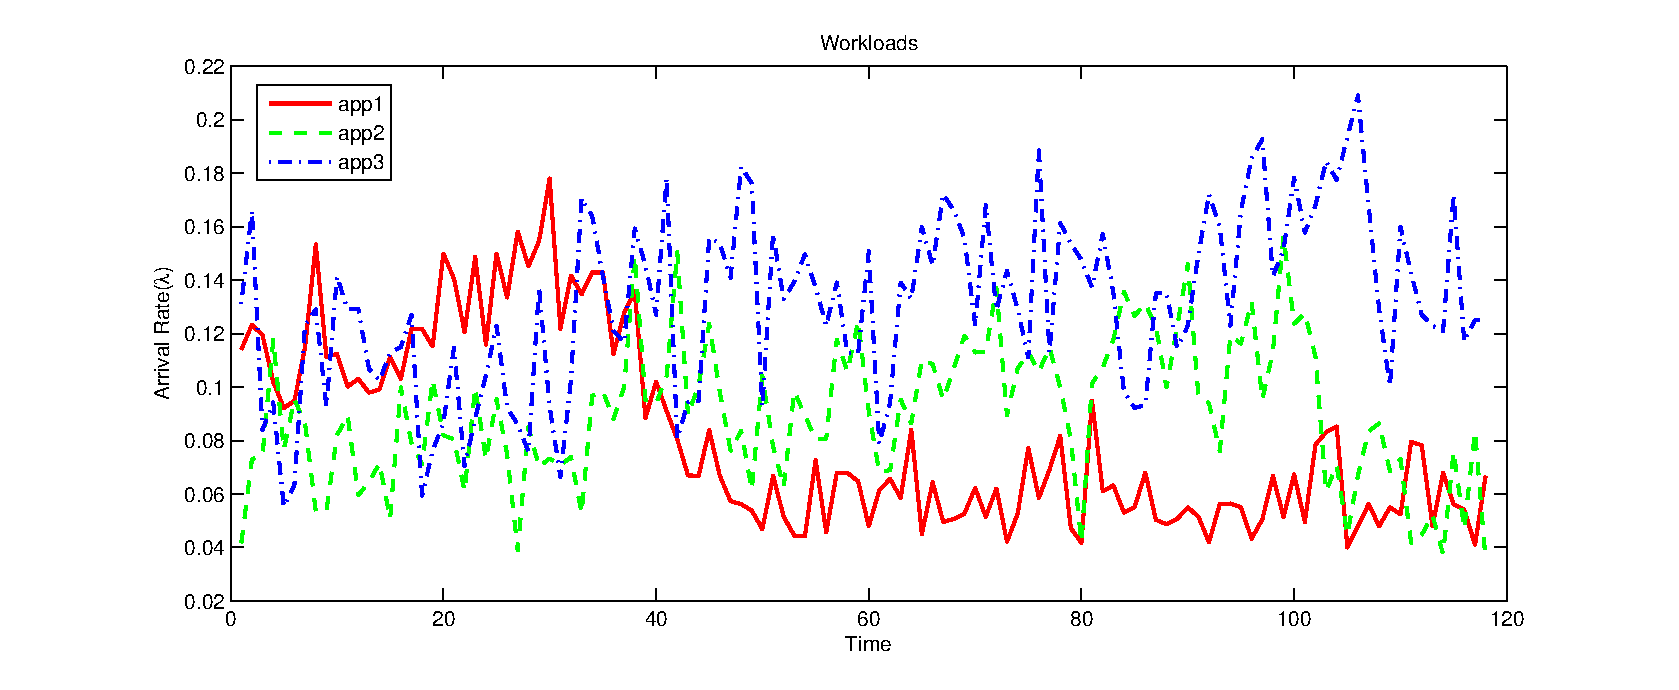
\includegraphics[width=1\textwidth]{image/centralized1/exp_simple_deploy-workload} 
\caption[A sample workload for the applications in a private cloud.]{The workload of applications. }
\label{fig:7}
\end{figure}

\begin{figure}
	\centering
\subfloat[][]{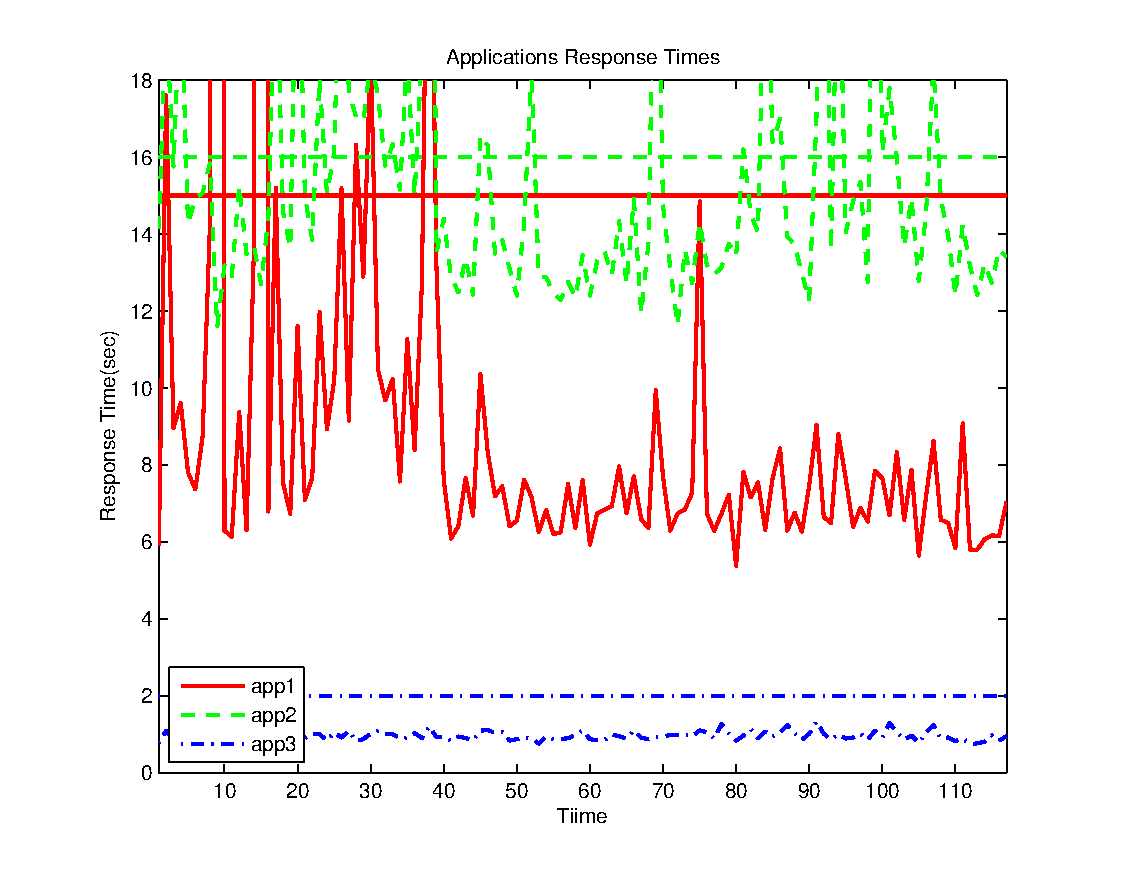
\includegraphics[width=0.5\textwidth]{image/centralized1/exp_simple_deploy-response_time}
\label{fig:3}}% (c) 
\subfloat[][]{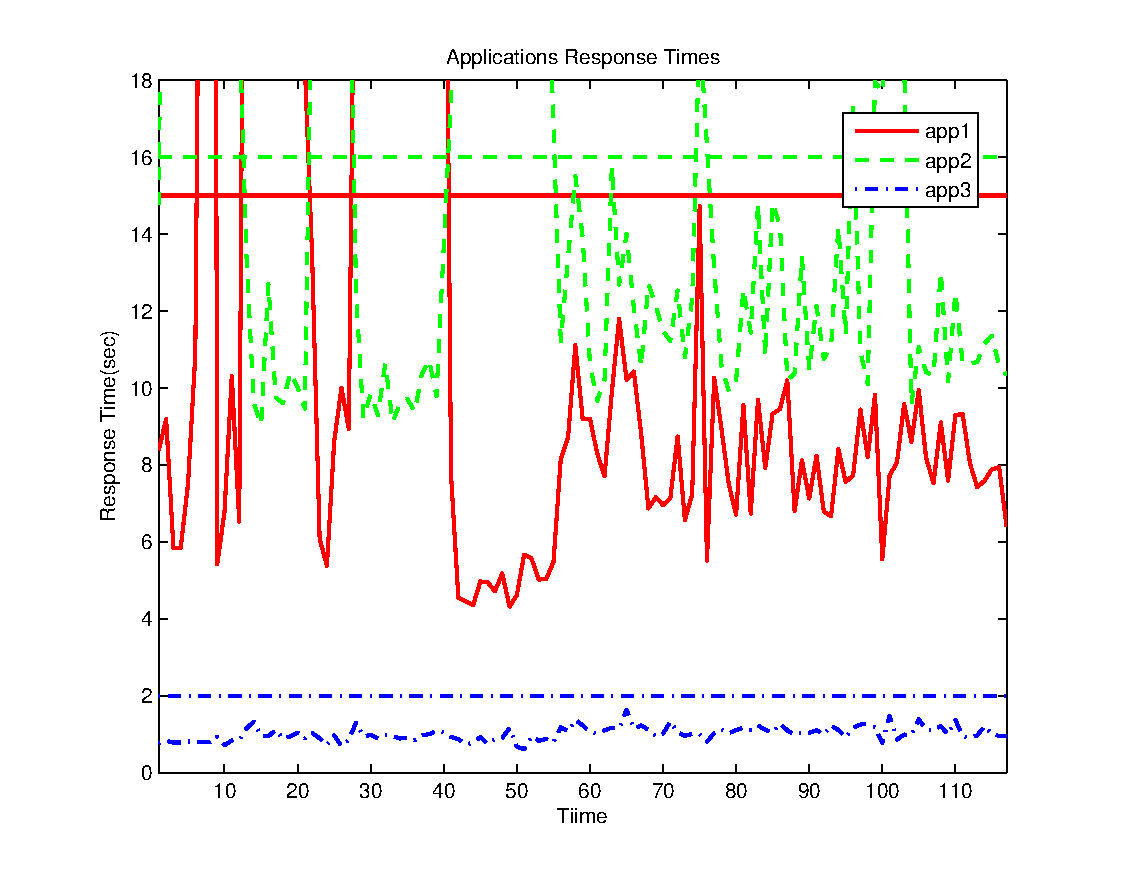
\includegraphics[width=0.5\textwidth]{image/centralized1/exp_simple_deploy_track-response_time}\label{fig:4}}% (d)
\caption[The achieved response time of applications in the simulated private cloud.]{The response time of applications together with SLA response times for \protect\subref{fig:3} static and \protect\subref{fig:4} dynamic models.}
\end{figure}

\begin{figure}
	\centering
\subfloat[][]{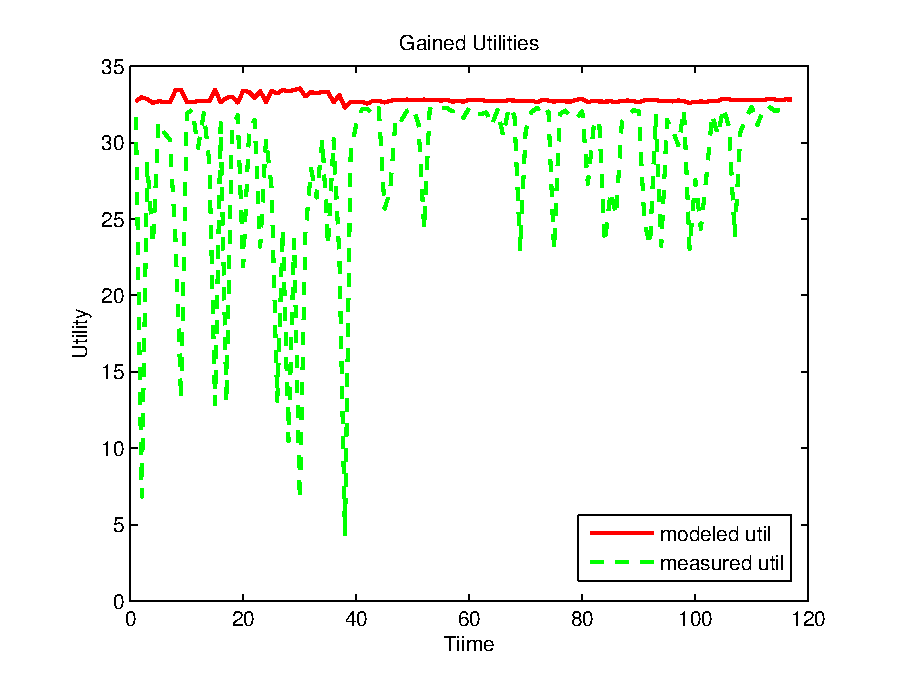
\includegraphics[width=0.5\textwidth]{image/centralized1/exp_simple_deploy-utility} 	
\label{fig:1}}% (a)
 \subfloat[][]{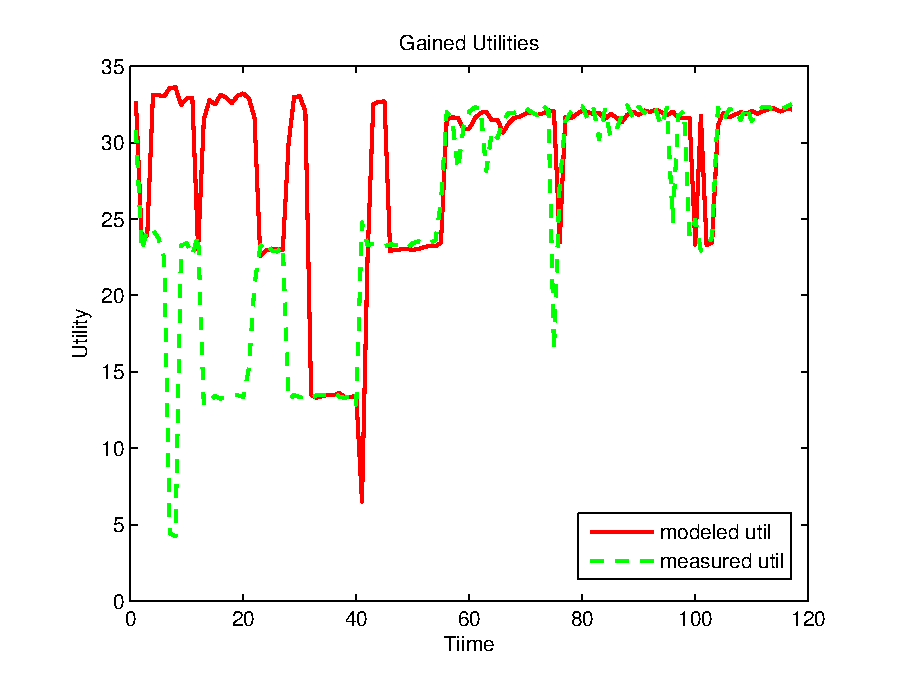
\includegraphics[width=0.5\textwidth]{image/centralized1/exp_simple_deploy_track-utility}\label{fig:2}}% (b) 
\caption[The measured and modelled gained global utility using static and dynamic models over time.]{The measured and modelled	gained global utility using \protect\subref{fig:1} static and \protect\subref{fig:2} dynamic models over time. } 
\end{figure}

\begin{figure}
	\centering
\subfloat[][]{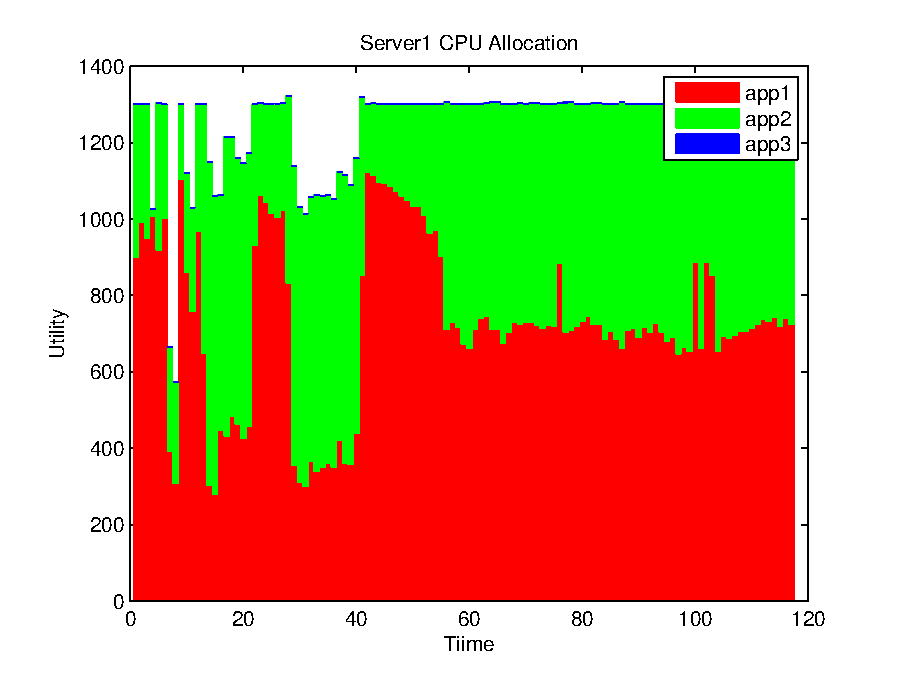
\includegraphics[width=0.5\textwidth]{image/centralized1/exp_simple_deploy_track-server1_cpu}\label{fig:5}}% (e) 
\subfloat[][]{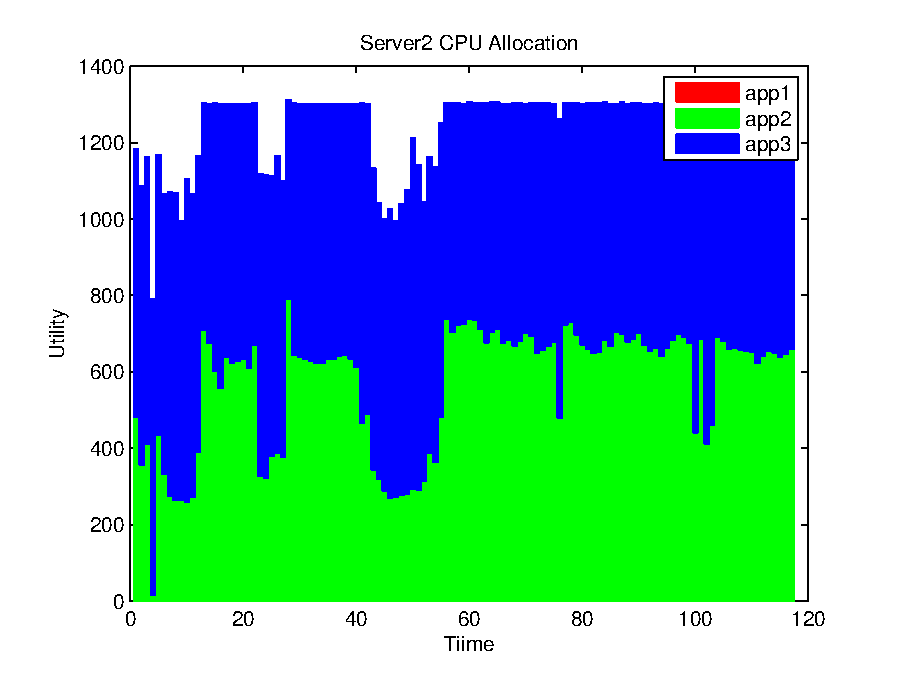
\includegraphics[width=0.5\textwidth]{image/centralized1/exp_simple_deploy_track-server2_cpu}\label{fig:6}}% (f) 
\caption[The allocated capacity to applications over time on server one and server two respectively using dynamic models.]{The allocated capacity to applications over time on \protect\subref{fig:5} server one and \protect\subref{fig:6} server two, using dynamic models. }
	\label{fig:case-study1}
 \end{figure}

% 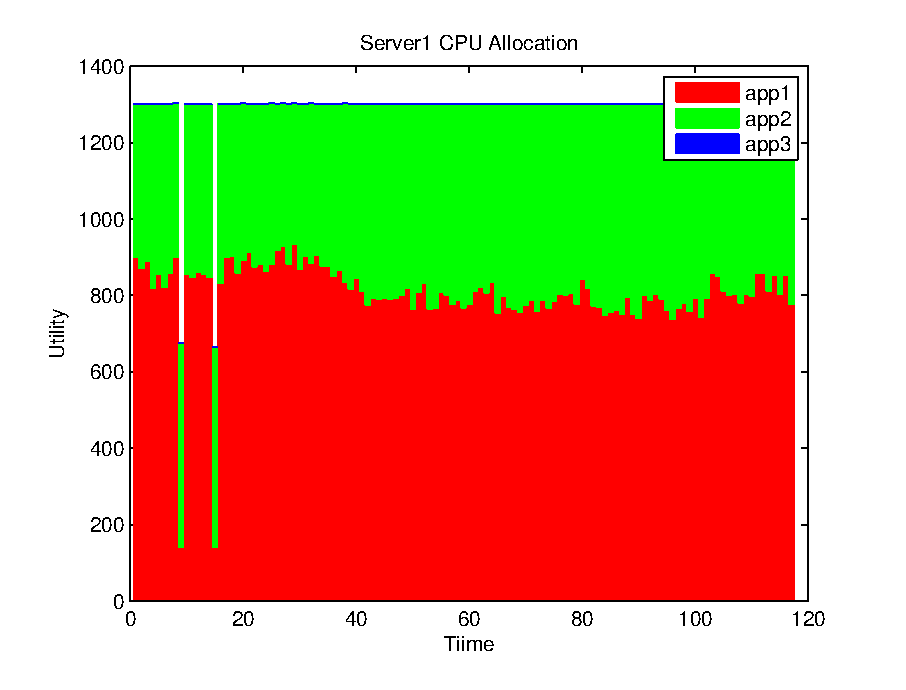
\includegraphics[width=0.45\textwidth]{exp_simple_deploy-server1_cpu}
% 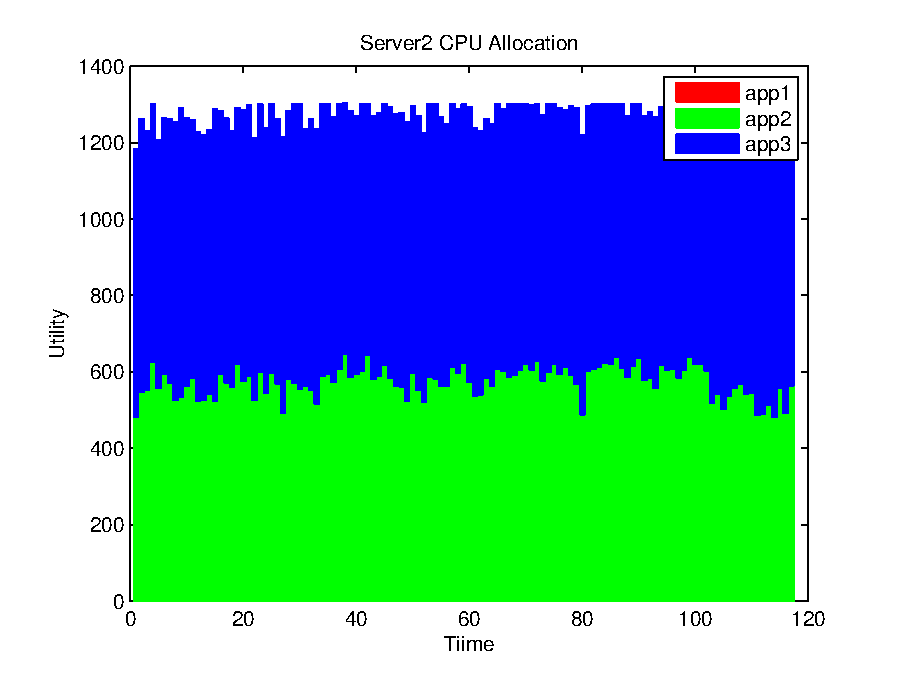
\includegraphics[width=0.45\textwidth]{exp_simple_deploy-server2_cpu}

\subsection{Case Study Two}
\label{sec:case-study2} 

The second case study was performed to demonstrate the ability of our approach to update the resource shares in a way that compensates for the additional workload. Ten applications were deployed on seven PMs.  VMs were assigned randomly to PMs.  All application workloads were set to have an inter-arrival time of 40 seconds except \texttt{app1} whose workload was monotonically increased (i.e., inter-arrival time was decreased from 40 to seven seconds).
\begin{figure}[h]
	\centering
	\subfloat[][]{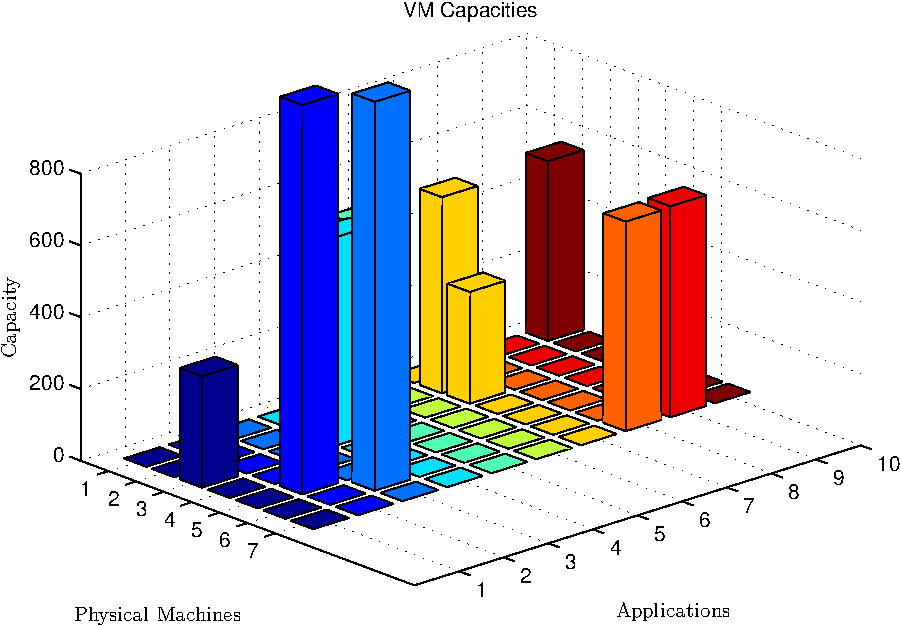
\includegraphics[width=0.5\textwidth]{image/centralized1/first_step}~\label{fig:case-study2-a}}
	\qquad
	\subfloat[][]{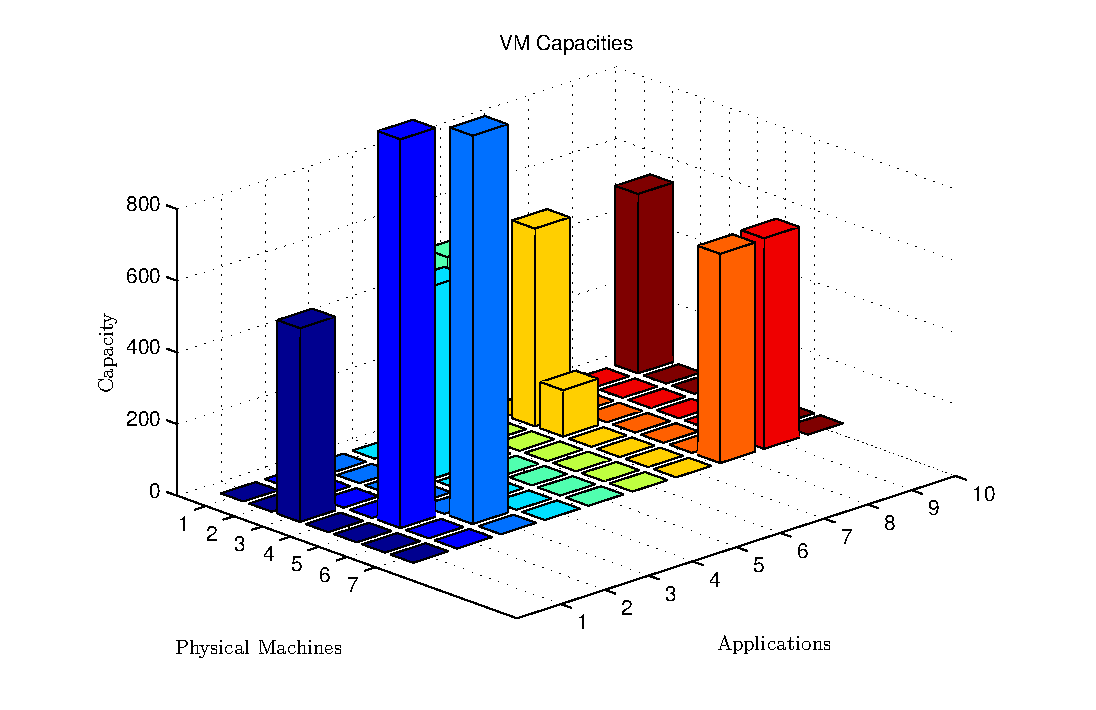
\includegraphics[width=0.5\textwidth]{image/centralized1/last_step}~\label{fig:case-study2-b}} %
	\caption[A snapshot of resource allocation both before and after an increase in the workload is detected.]
	{A snapshot of resource allocation both (a) before and (b) after an increase in the workload is detected.}	\label{fig:case-study2} 
\end{figure}
Figure~\ref{fig:case-study2} presents both before (a) and after (b) snapshots of resource allocations.  Note that both \texttt{app1} (dark blue) and \texttt{app7} (yellow) are resident on the same PM.  Initially, \texttt{app1} is allocated approximately 300 MIPS while \texttt{app7} is allocated approximately 310 MIPS. After the increase in the workload, \texttt{app1} is allocated approximately 510 MIPS while \texttt{app7} is allocated approximately 100 MIPS.

\subsection{Assessing the Scalability}
 In addition to the experiments performed in cases studies one and two, the relationship between the number of simulated VMs and the optimization time per step was also considered and a non-linear but polynomial relation was observed (see Figure \ref{fig:scalability}). 
\begin{figure} 
	\centering
	  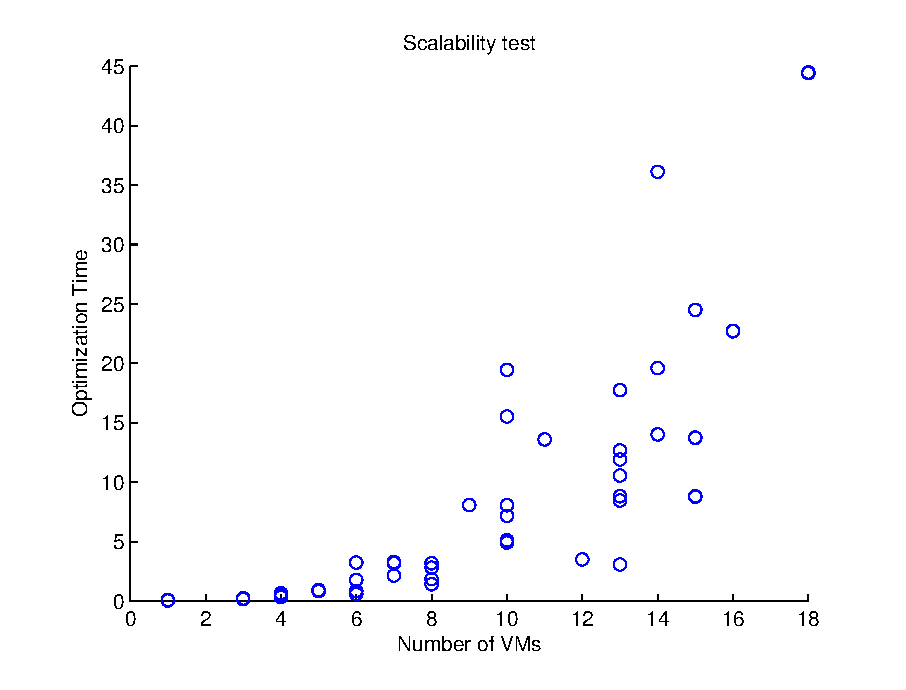
\includegraphics[width=0.8\textwidth]{image/centralized1/scalability}		
	\caption{The relationship between the number of simulated VMs and the optimization time for each optimization step.}%
	\label{fig:scalability} 
\end{figure}

\section{Summary}  
\label{sec:future-work}
The purpose of this chapter was to demonstrate the advantage of ``adaptive empirical'' models relative to ``static empirical'' models in resource management.  
We investigated dynamic tuning of empirical resource allocation models. 
We described an approach which dynamically updates an empirical model for each application at runtime in order to capture the effects not considered in the initial specification of the model. 
This dynamic updating results in more accurate estimates being passed to the optimizer, allowing for better resource utilization on a global scale.  
We traced the effect of this tuning, in the overall system performance. We showed, in terms of performance, dynamic adjustment of model parameters using an EKF, can outperform a model built off-line using a non-linear regression. 

% We also investigated the model based optimization of resource shares in a private cloud where applications are distributed across a set of PMs. The goal was minimizing the SLA violations. While we focused only on the response time, considering other service level objectives would not change the approach (just the complexity of solving the optimization problem). 

% Future work will involve implementing the optimization algorithm in a distributed manner, in which applications interact in a peer-to-peer fashion to determine how much resource should be allocated to each. One can also investigate optimizing the dual optimization problem, which is more suitable for mapping to an agent-oriented optimization approach (see \cite{huang_macroeconomics_2008,izakian_auction_2010}).


  


\chapter{Optimal Service Replica Placement via Model Predictive Control}
\label{ch:replica_placement_through_mpc}    
%\begin{center}
%\textbf{This chapter contains material from Ghanbari et al. \cite{ghanbari2014mpc}}.
%\end{center}

This chapter presents a dynamic service placement algorithm for Optimal Service Placement (OSP) of a set of N-tire software applications. The algorithm solves an optimization problem in each control step. 
The solution of the optimization suggests that some service replicas be added or removed from the available hosts. These deployment changes are optimal with regards to overall long-term objectives. In addition, the optimization considers restrictions imposed on the number of possible service migrations at each time interval.  

%In the second part of this chapter, we propose a technique to for finding the optimal of reservation actions to minimize cost in a public IaaS cloud environment. The problem here was to reserve enough number of hosts preemptively to accommodate the workloads. The optimality of our approach is only guaranteed if the hosts are homogeneous, that is the cloud only offers one type of resource.\footnote{Note that this differentiates this problem from the optimal selection of active hardware components.}  With more types of hosts, the optimization problem becomes an integer programming. Thus, we use a heuristic in case of multiple resource types that only achieves a sub-optimal solution.

%\begin{spacing}{1} 
% \begin{algorithm}
%        \small
%        \SetAlgoVlined
%        \SetKwInOut{Input}{input}e
%        \SetKwInOut{Output}{output}
%%        \SetKwInOut{Initialize}{initialize}
%        \SetKwInOut{Variables}{variables}  
%  \SetAlFnt{\tiny}
%\Input{desired response times regarding customer classes}
%\Output{optimal placement $u$ and reservation actions for current step }
%\BlankLine
%in each time interval: 
%  estimate workload component (N,Z,D)  and host capacity (mu)? and throughput x (if unobserved) using accurate QM. \\
%  calculate the system necessary throughput to support the workload component \\ % using N, Z translate the target R into X 
%  calculate the NFM demands (d) based on the observed/estimated throughputs, capacities ? \\
%  plan the resource reservation and/or allocation actions for current time interval  \\
%\caption{hi}
%\label{algorithm1}
%\end{algorithm}
%\end{spacing}  

\section{Problem Components}  
The definition of the OSP problem includes five components: hardware structure, software structure, workload, infrastructure cost, and QoS related Service Level Objectives (SLOs). The solution to the problem is an optimal set of placement changes at each timestep during the lifetime of a cloud provider. 
Each placement change is an addition or deletion of a service replica to or from a host in a data center. In the rest of this section, components of the problem are briefly discussed:  
  
\subsection{Hardware structure} We assume a cloud with heterogeneous resources composed of $H$\nomenclature[M]{$H$}{Number of hosts in a data center} hosts. Each host has a number of resources such as disks, random access memory (RAM), and processors. We assume there are $K$\nomenclature[M]{$K$}{Number of different types of resources in a data center (i.e. the CPU, disk, and the network)}\footnote{We use an uppercase letter to denote the number of instances of an entity while using lowercase letters for indexing individual instances.} of these types of resources within the data center\footnote{Note that besides hosts, a data center is also composed of a network and a storage fabric. Although the theory developed here can be tailored for those as well, these resources are not addressed in this chapter. }. The multiplicity of resource $k$\nomenclature[M]{$k$}{Index of type of resource} of a host $h$\nomenclature[M]{$h$}{Index of a host}
 is denoted by $\capp_{h,k}$\nomenclature[M]{$\capp_{h,k}$}{The multiplicity of resource type $k$ of host $h$}. If the only resource under consideration is the CPU, then the multiplicity can be simply written as $\capp_{h}$. Each host resource is also associated with speed factor $\speedFactor_{h,k}$. If the only resource of consideration is the CPU, then speed factors are written as $\speedFactor_{h}$. 

\subsection{Software structure} We assume the system is composed of $S$\nomenclature[M]{$S$}{The number of services in the data center. } services. The software structure is modelled based on interactions of these services. We quantify these interactions using two sets (also elaborated in subsection \ref{sec:workload-demands-background}):  
 (i) The service demands of the services on different resource types of data center hosts. 
 (ii) The service call graph, where each edge from a caller service to a callee is labeled by the number of invocations for each execution of the caller. 

\subsection{Workload} The workload component was described in subsection \ref{sec:workload-background}. The workload component it is represented by $C$ classes of users that make use of the shared services. Each class $c$ of users is identified by: (i) it's number of consumers, $N_c$, and it's think time, $Z_c$, as discussed in subsection \ref{sec:workload-intensities-background},  (ii) the number of visits from classes to front-end services derived from CBMG is $V_{c,s}$, denoted for each class $c$ and service $s$.   

\subsection{Infrastructure cost} The infrastructure cost is  based on energy consumption  and is modelled as a function of resource utilizations. 
   
\subsection{Service level objectives} An SLO for each application (or class of users) is represented by an upper bound on the application's response time $R_{c}^\text{SLA}$ \nomenclature[M]{$R_{c}^\text{SLA}$}{SLO upper-bound on the response time of class $c$.} or lower bound on its throughput $X_{c}^\text{SLA}$.  \nomenclature[M]{$X_{c}^\text{SLA}$}{SLO lower bound on the throughput of class $c$.} 
As an example, consider a service center composed of 14 services ($S=14$), accessed by 2 classes of users ($C=2$). 
Figure \ref{fig:service_call_graph} represents the call graph of the services and 
the number of visits from the classes to services ($V_{c,s}$); 
the think times ($Z_c$) and 
the number of users ($N_c$)\nomenclature[M]{$N_c$}{Number of users in class $c$} of each class over time, and 
the invocation numbers within services ($y_{c,s}$). 
% see this http://old.nabble.com/Two-lables-on-a-node-(one-outside)-td31349791.html
\begin{figure}[htbp]
\begin{center}
 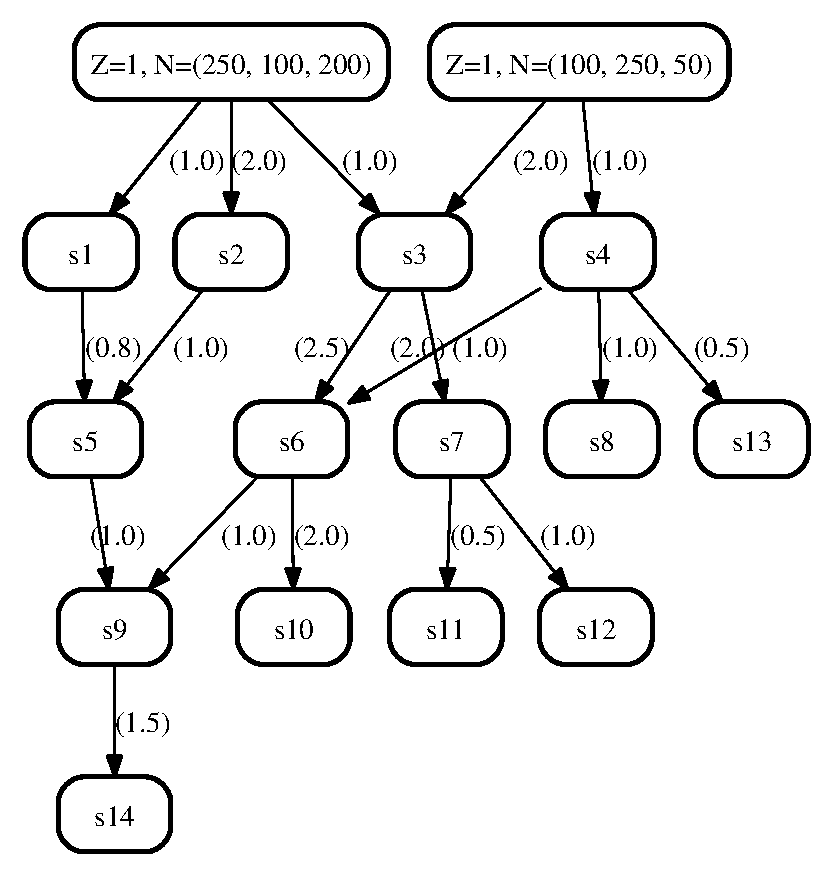
\includegraphics[scale=0.8]{image/placement/example1services}
 \caption[An example small scale service center.]{An example small scale service center: the call graph of services and classes, the number of calls from classes to services (a portion of $y$)\nomenclature[M]{$\servMeanReq_{es}$}{Mean requests made directly from any service $e$ to service $s$}, the invocation numbers within services (another portion of $y$), the think times ($Z$) and the number of users ($N$) of each class over time. }
\label{fig:service_call_graph}
\end{center}
\end{figure}
There are 6 available hosts to support the services. Capacity of the hosts are  $\capp=[16\ 6\ 6\ 16\ 6\ 6]^T$ and their CPU speed factor is $\speedFactor=[1\ 1.2\ 0.9\ 1.1\ 0.8\ 1.2]$. 
Hosts are initially unallocated, and no replica is deployed on them. % : $\theta_{s,h,0} = 0 \text{   for all $s$,$h$.}$

\section{Motivating Example}    
\label{sec:motivating-examples}   

% A Comparison of the Optimal Control and the Step-by-Step Optimization, a Hypothetical Case of a Fully Known Workload     
 In this section, using a simple example, we show the effect of solving a service placement problem using then optimal control framework. We show that if the objective is to avoid reconfiguration (i.e. there is a cost to service replication changes), and the workload has oscillations, the model predictive control provides better results than stepwise optimization. 

Consider the problem of service placement in a small-sized service center where the objective is to minimize the hosting costs and to minimize the total number of relocations while meeting the multi-class workload response time goals. 
There is a random resource cost coefficient associated with each host. The response time SLA for all the steps were set to $R^\text{SLA}_t = [0.146 \  0.267]^T$. The $R^\text{SLA}_t$ specifies the upper bound on the response time values for classes, namely $R^\text{SLA}$.

Assume a three step-ahead prediction of the mean number of users given the observations up to now ($E[N_{c,t+k}|N_{1:t}]$) is provided through some statistical prediction technique: % ; in some form such as a Dynamic Linear Model (DLM).  
% \footnote{given the fact that number of users can be non-stationary and might not have seasonal or linear trends, we could not use models such as ARIMA}:  
% The workload for this example was considered to be: 
\[
N=\left(\begin{array}{ccc} 
220.0 & 150.0 & 200.0\\ 
100.0 & 170.0 & 110.0 \end{array}\right)
\]
 where each row represents a class of users, and each column represents a future timestep. 

 The optimization was applied in two settings: (i) solving a set of individual optimizations for separate steps ignoring the transition cost (step-by-step optimization) and (ii) solving for all the steps in one optimization problem considering the cost of reconfiguration (overall optimization).            

 In the step-by-step optimization, the optimizer achieves the desired throughput by an initial deployment of 18 replicas in the first step and a total addition of 9 and removal of 11 in the subsequent steps (total changes of 38). The placements are depicted in Figure \ref{fig:stage_based_optimal_example}. 
The undirected blue dashed lines denote the placements that have been added in the corresponding steps, and the red dashed lines represent the placements that have been just removed at each time step. The black dashed lines denote the placements performed in the past time steps. 

The excessive number of service reallocations in this case are because the optimizer targets the least cost configuration (based on the host coefficients) without taking into account the cost of relocations. The removal and addition of services incur a reconfiguration cost and network overhead, and thus makes this solution suboptimal. 

Note that associating cost with the number of relocations in the current step, in case of step-by-step optimization, will not solve the problem.  This is because the effect of the relocations propagates through future steps (depending on the future workload). 

\begin{figure}[h]
\begin{center}
\subfloat[Overall optimal example][Initial placement decision (at $t=1$)]{ 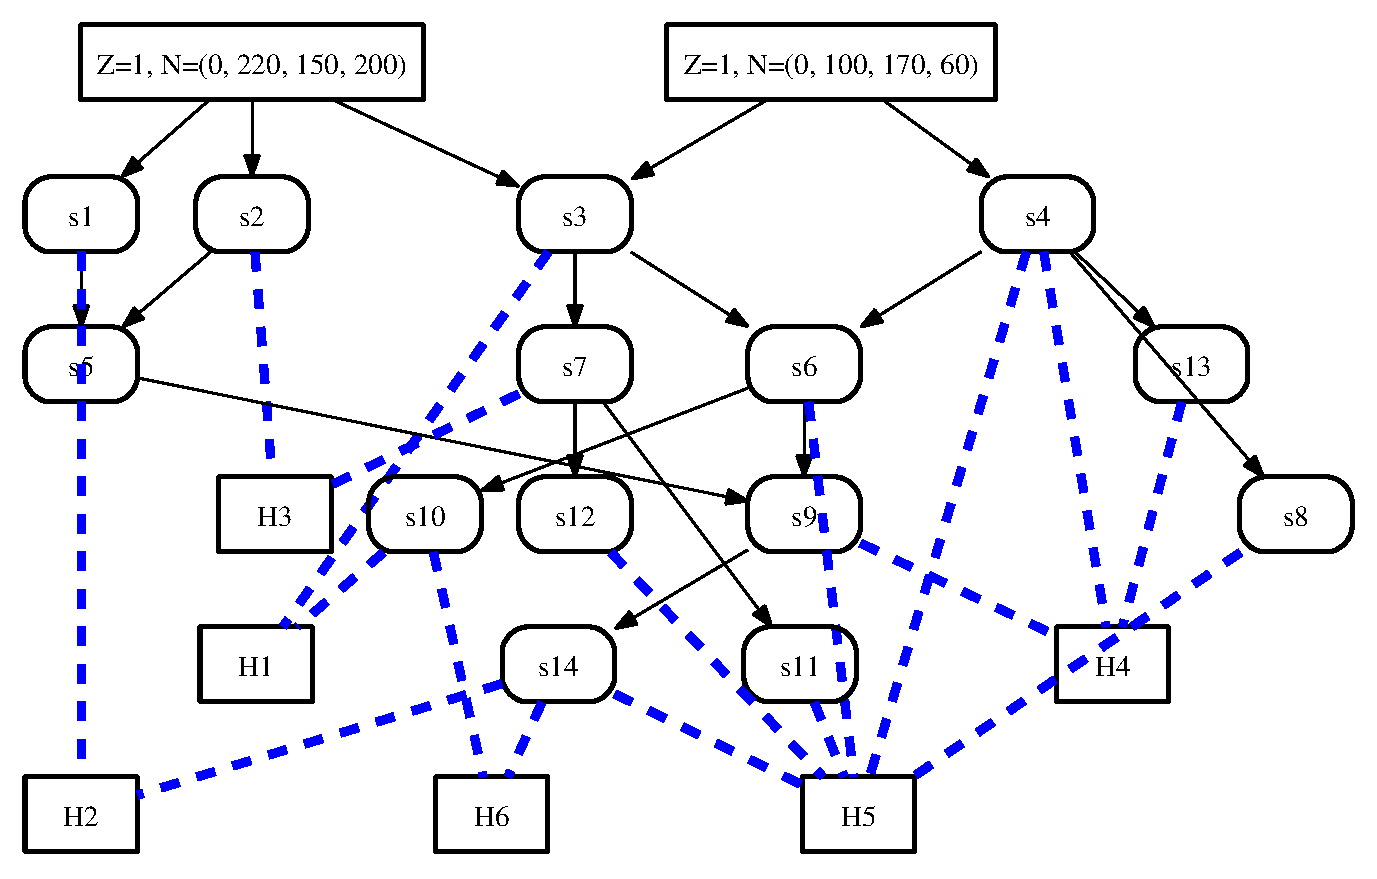
\includegraphics[width=0.4\textwidth]{image/placement/example1deployment_step1} \label{fig:subfig1}}  
\qquad  
%
\subfloat[Subfigure 1 list of figures text][Placement decision at $t=2$]{
 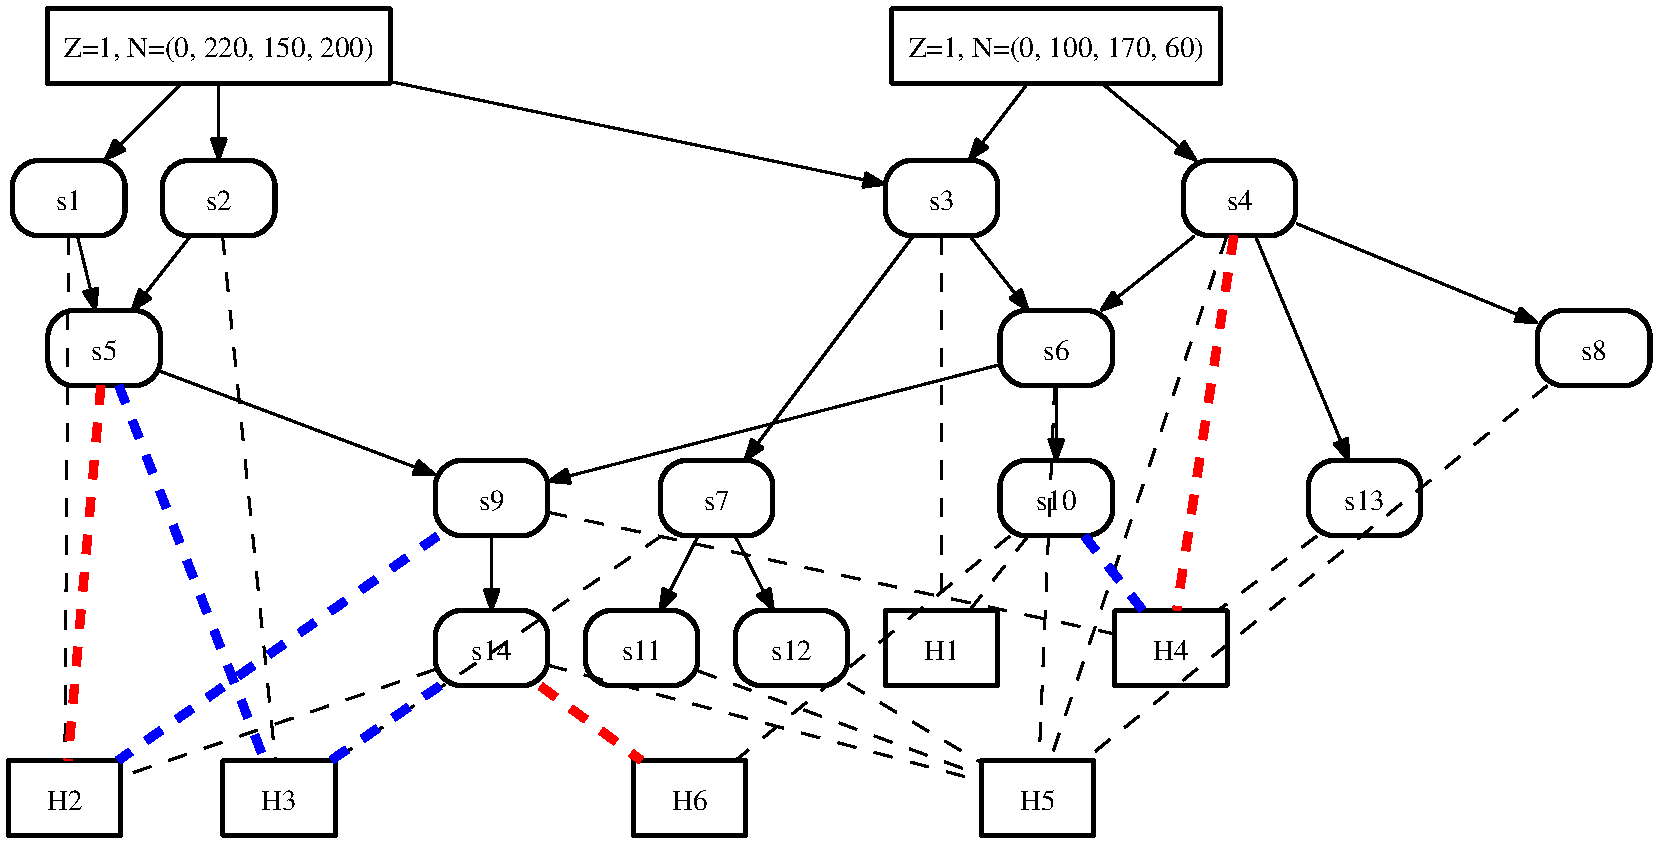
\includegraphics[width=0.5\textwidth]{image/placement/example1deployment_step2} \label{fig:subfig2}} 
  \qquad
%
  \subfloat[Subfigure 1 list of figures text][Placement decision at $t=3$]{
 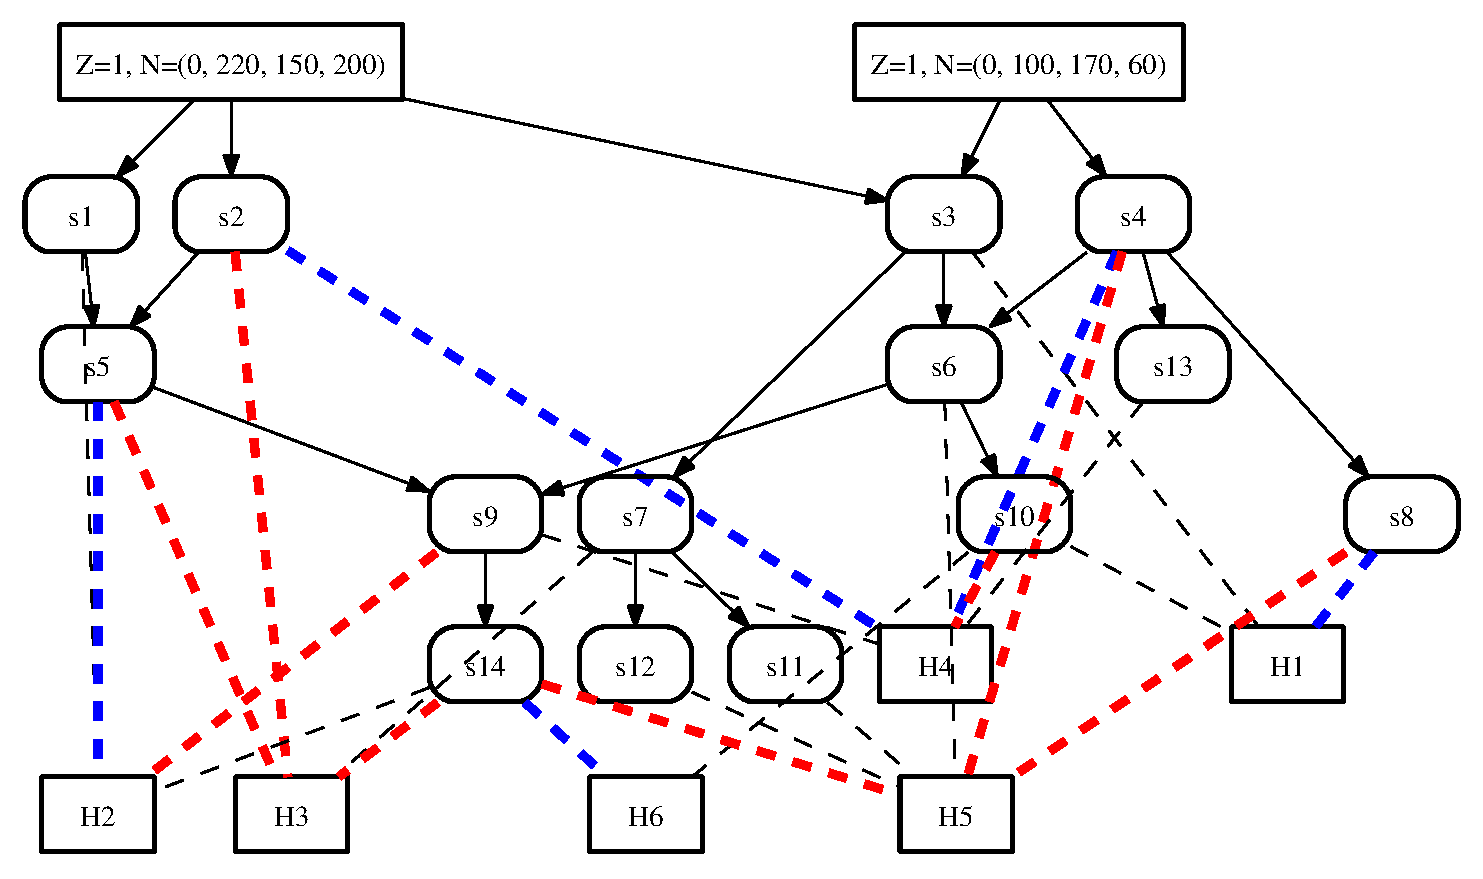
\includegraphics[width=0.5\textwidth]{image/placement/example1deployment_step3} \label{fig:subfig3}} 
 %
\caption[An example of placement decisions for a small service center using step based optimization, ignoring the future steps.]{An example of placement decisions for a small service center using step based optimization, ignoring the future steps.} 
\label{fig:stage_based_optimal_example}  
\end{center}
\end{figure}  

 In the overall optimal case, the desired throughput is achieved by an initial deployment of 19 service replicas in the first step and the total addition of 0 and the removal of 0 in the subsequent steps (total changes of 19). Although this solution is not as efficient in terms of the resource cost, 
it has a better total cost since it also considers the relocation cost. 

%The placement decisions at $t=0$ (which is maintained through $t=1$ and $t=2$) is demonstrated in Figure \ref{fig:overal_optimal_example}. 

%\begin{figure}[htbp]\begin{center}\subfloat[Overall optimal
%example][Initial placement decision (decision at
%$t=1$)]{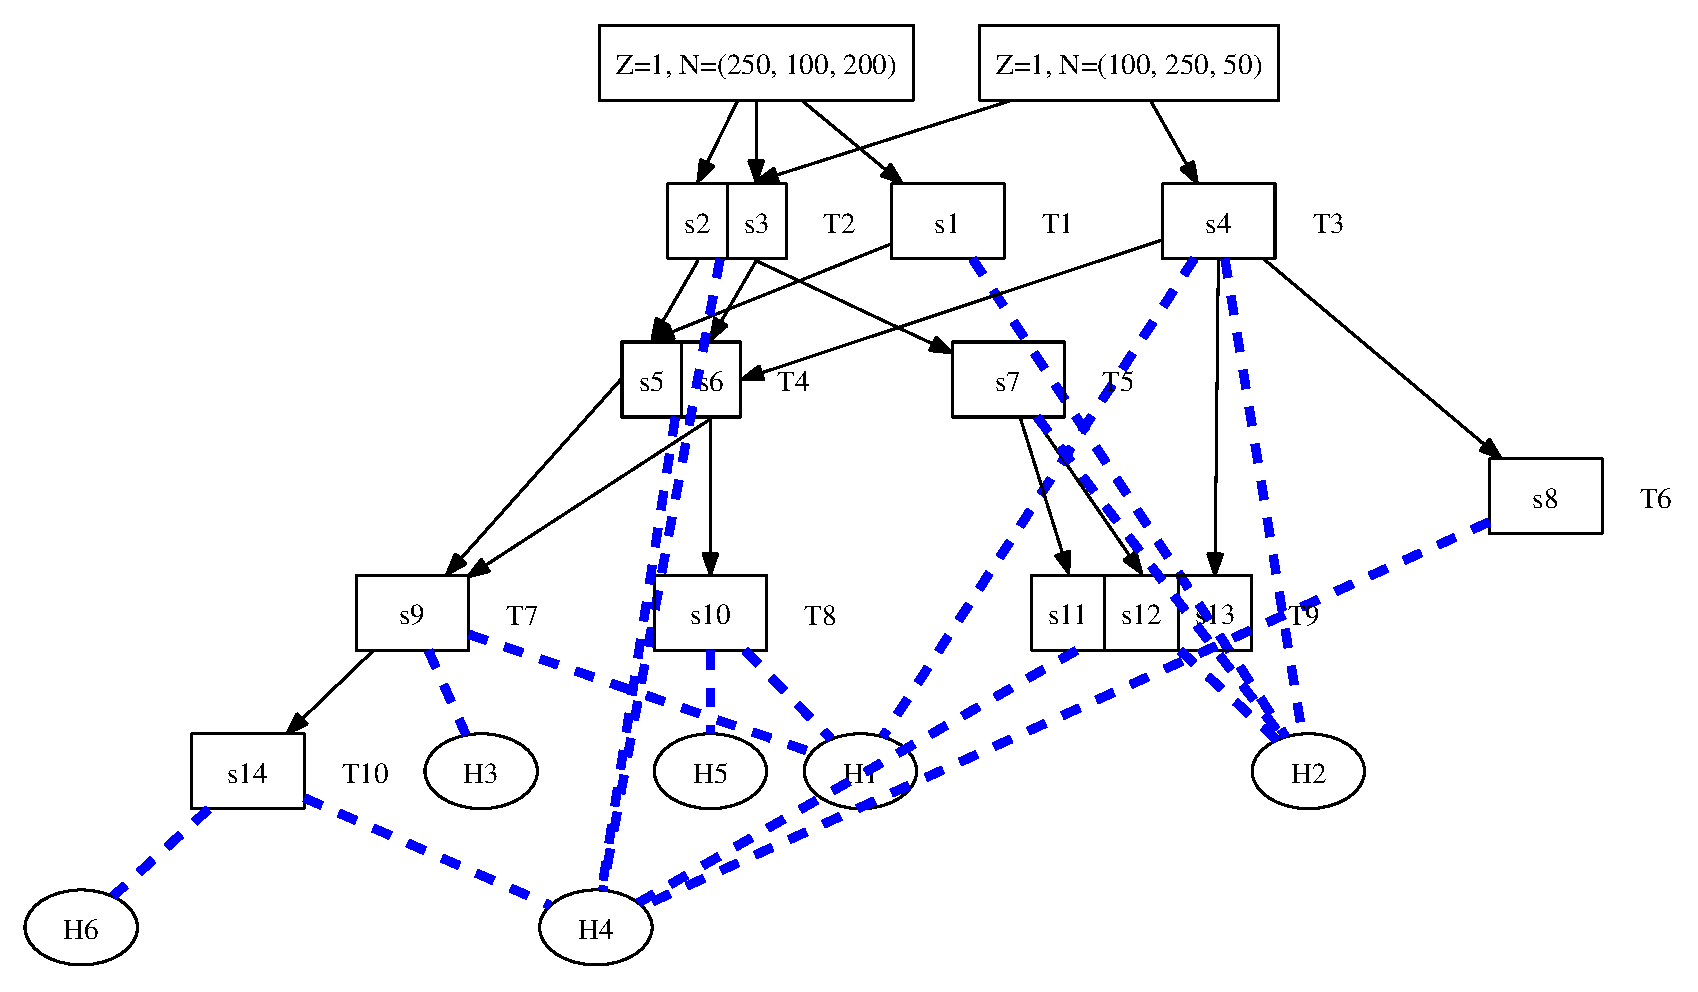
\includegraphics[scale=0.4]{image/example1deployment_overal_step1}
%\label{fig:subfig1}}
%\caption[Represents the placement decisions for a small service center
%using the optimal control.]{Represents the placement decisions for a
%small service center using the optimal control.
%}\label{fig:overal_optimal_example}\end{center}\end{figure}%

%\subsection{Example 2} 
Note that, in this example we assumed a prediction of the future mean workload conditioned on the past values is available through statistical modeling. 

% here is the example  about adding a class of service
%In this example, we show a case that a new class of services is added to the system. Consider the same small size service center. Let us assume that the system is already stabilized to the $N_{c1}=160$ users of class $c1$ with response time goal of $R^\text{SLA}_{c1}=0.146$. The class c2 joins the system at $t=1$ with a population of $N_{c2}=100$ and a SLA of $R^\text{SLA}_{c2}=1.146$. 
%The initial workload of the class of service is estimated and the load is assumed constant for the model predictive look-ahead window. Still the MPC will provide a better result than a static one-step optimization because it can distribute the necessary changes over time in a way that it better satisfies the overall objective.
	%
	%We performed a simulation of $J=100$ steps that captures the behaviour of a controlled service center until it converges to a steady-state value.   
  %
 %Figure \ref{fig:adding_class_serv_portion} shows the amount of resource given to each service, which is increased for all of the services after the 2nd class is added to the system. 
 %Figure \ref{fig:adding_class_throughput} presents the throughput of the classes. 
  %As noted  it takes around 7 steps for the throughput of the class c2 to reach its SLA value. The duration of this convergence depends on the reconfiguration cost coefficient which has been set it to $r_3=100$.  
    %
%\begin{figure}
%\begin{center}
%\subfloat[Service addition scenario, amount of resource given to each service][Amount of resource given to each service]{
 %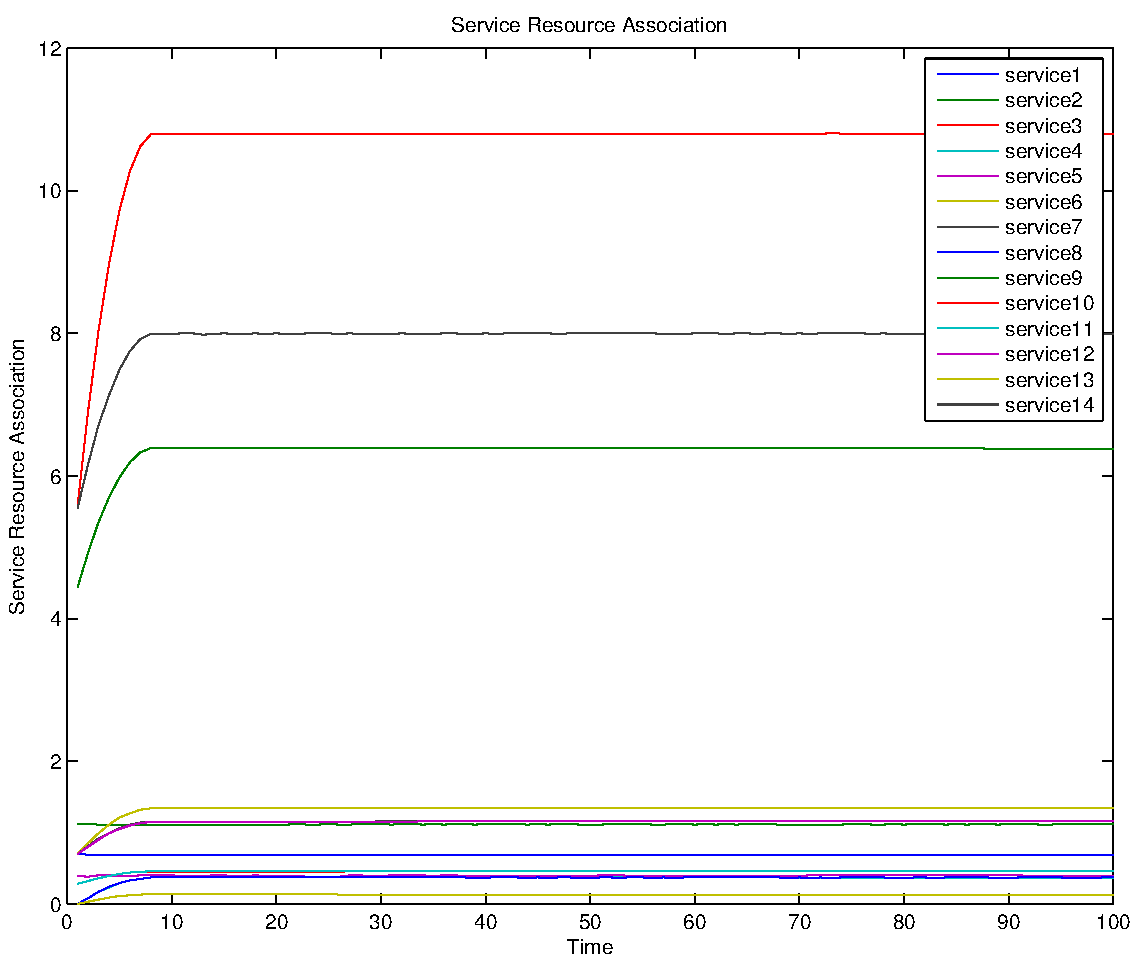
\includegraphics[scale=0.4]{image/placement/adding_class_serv_portion} \label{fig:adding_class_serv_portion}} 
  %\qquad
  %\subfloat[Service addition scenario, the throughput of classes][ the throughput of classes]{
 %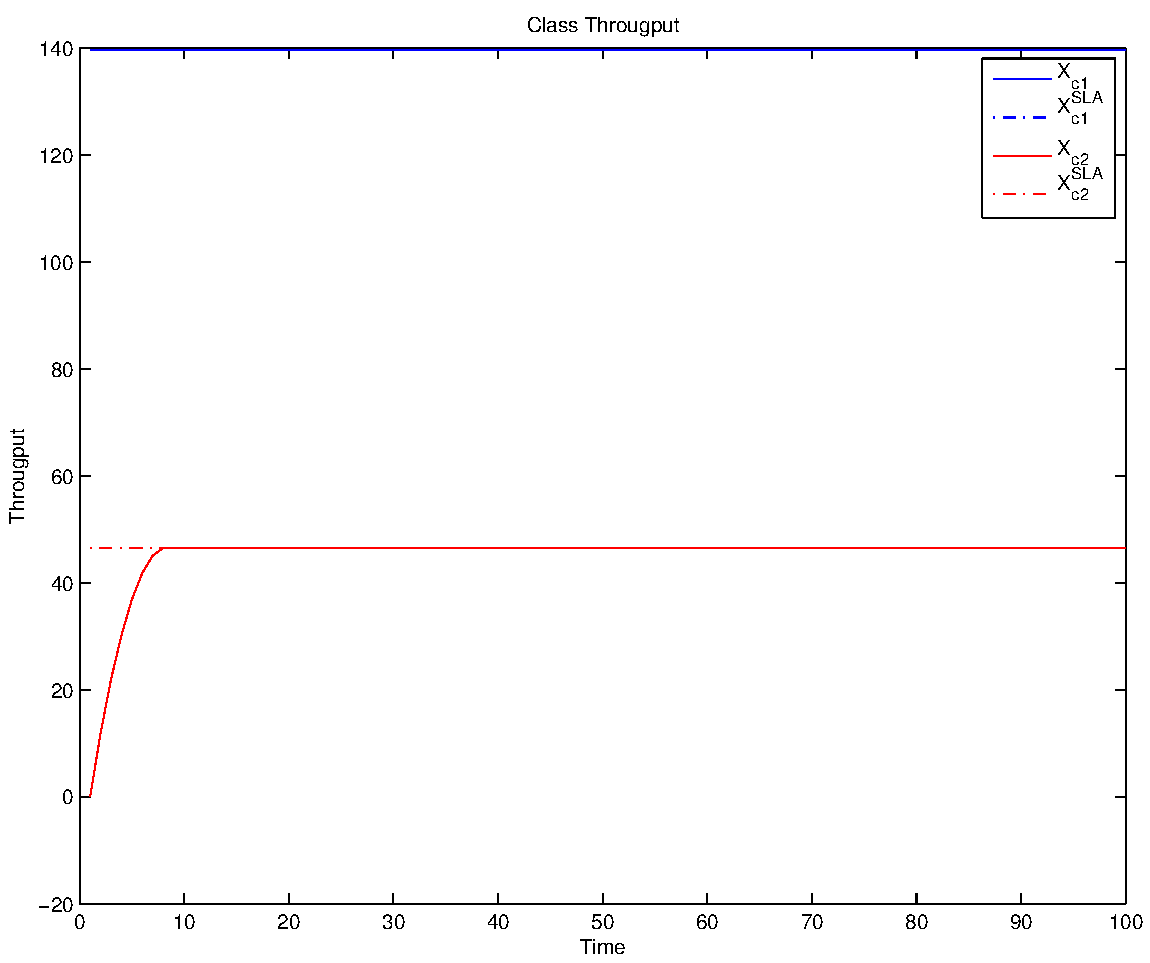
\includegraphics[scale=0.4]{image/placement/adding_class_throughput} \label{fig:adding_class_throughput}} 
%\caption[Placement controller response to arrival  of a new class  of users]{Placement controller response to arrival  of a new class  of users. }
%\label{fig:stage_based_optimal_example}  
%\end{center}
%\end{figure}
     
\section{Problem Formulation}  
\label{sec:problem-formulation}  
  Having the above set of inputs, we can formulate the problem as follows:    
 assume a three-dimensional array or tensor $\theta$, whose elements are denoted by $\theta_{s,h,t}$, represents the placement of the replicas of the services on the available hosts over a time horizon\nomenclature[M]{$t$}{The timestep index}.
 In fact, each $\theta_{s,h,t}$ denotes the portion of service $s$ that is allocated to a host $h$ through a placed replica and a proper routing at a time $t$. As a result, we have: 
 \begin{align} 
&  \sum_{h=1}^H \theta_{s,h,t} = 1 & \qquad \text{for each $s$ and $t$} \label{eq:thata_totals_to_one}   
 \end{align}     
 In other words, at each time step $t$, $\theta$ represents a $H\times S$ bipartite graph  of the associations between the hosts and the services. 
 The actual demand on each resource is obtained by taking into account this association of the services and the hosts ($\theta_{s,h,t}$) \nomenclature[M]{$\theta_{s,h}$}{The portion of service $s$ that is handled by host $h$ through a placed replica and proper routing.} as:
 \begin{align} 
      %  &  d_{c,s,h,t} =  
 d_{c,s,k} \theta_{s,h,t}			\qquad & \text{for each $c$,$s$,$h$,$k$,$t$  }    
	 \label{eq:thata_as_proportion}   
 \end{align} 
  %    here $d_{c,s,h,t}$
  This expression gives the demand of class $c$ on a resource type $k$ of a server $h$  through service $s$ at time $t$, and $\theta_{s,h,t}$  denotes the portion of service $s$ that is associated to host $h$ through a placed replica and proper routing. 
 Focusing only on the CPU resource, one can drop the index $k$ representing the resource type from $d_{c,s,k}$, for simplicity. 
 For service $s$, a desired $\theta_{s,h,t}$ at time $t$ can be achieved by dividing the service invocations made to $s$ between its service replicas proportional to $\theta_{s,h,t}$ (taking $h$ as the variable):  
   \begin{align}
    y_{e,s,h} =   \theta_{s,h,t}  y_{e,s} 
   \end{align}
   where $y_{e,s,h}$ denotes the call multiplicity from each service $e$ to a replica of $s$ on $h$. $\theta_{s,h,t}$ is, in fact, the proportion of the service $s$ requests routed to its replica on the host $h$ at time $t$. 
	If for some $s$ and $h$, $\theta_{s,h,t}=0$, then there will not be any replica of service $s$ on host $h$ at time $t$. Thus, $\theta$ represents both the deployment and the quantity of resource allocation. 
 
  The cost to a cloud provider depends on the number of active hosts utilized over the providers' lifetime. The fewer active hosts used, the less cost will be incurred. 
  Indirectly, the cost depends on the placements during the provider lifetime (i.e. $\theta_{0},...,\theta_T$)\nomenclature[M]{$\theta_t$}{Placement of services on hosts at timestep $t$.}, where the provider lifetime is denoted by $T$\nomenclature[M]{$T$}{A lifetime of a cloud provider in the context of a control problem (possibly infinite).}.  

 The problem is choosing a sequence of optimal placements $(\theta^*_0,...,\theta^*_T)$ that minimizes the long term resource cost while trying to satisfy the SLOs over time. In summary, the problem is the optimal deployment of the service replicas on the available hardware over time: 
\begin{equation}
  \begin{aligned}
\underset{\theta_0,...,\theta_{T-1}} {\text{minimize } } 
   E \Bigg[ 
		 &\rSLA \sum^{T}_{t=1} \sum^C_{c=1}   \lambda_\text{SLA}(R_{c,t} - R_c^\text{SLA})   \\
   + & \rResource \sum^{T}_{t=1} \sum_{h=1}^H \lambda_{\text{resource},h}(U_{h,t})  \\
   + & \rDeployment  \sum^{T}_{t=1} \sum^H_{h=1}  \sum^S_{s=1} \lambda_\text{dep}(\theta_{s,h,t},\theta_{s,h,t-1}) \Bigg]  \\ 
\text{subject to:} \nonumber \\ 
 & R_{t} =  \text{LQM}_{\Omega,\speedFactor}(d_{t},\theta_{t}, W_{t})  &  \forall t  \\ 
 &  \sum_{h=1}^H \theta_{s,h,t} = 1 &  \forall s , t
\label{eq:opt-overall-abstract}
    \end{aligned}
\end{equation}

%
\nomenclature[M]{$\lambda(\alpha_t)$}{The cost of resources at time $t$.}
\nomenclature[M]{$u_t$}{Change in the placement made at time $t$.}  
\nomenclature[M]{$E[...]$}{An expected value.}   
\nomenclature[M]{$J_2$}{The cost of cloud provider, containing both costs of infrastructure and SLA violation.}    
Here, $T$ denotes the service centre lifetime. $(u_0,...,u_{T-1})$ is the service placements performed during this lifetime. $E\left[...\right]$ represents an expected value. $\rSLA$, $\rResource$, and $\rDeployment$ respectively represent the coefficients associated with the cost of violating SLAs, the cost of hardware resources, and the cost of changes in the deployment of services. These coefficients ($\rSLA$, $\rResource$, and $\rDeployment$) are used to tune the trade-off between the different cost factors. The expression $\lambda_\text{SLA}(R_{c,t} - R_c^\text{SLA})$ represents the cost of violating the SLO for a class $c$ at time $t$. 
Note that the SLO is defined only based on the response time of the class $c$ at each timestep (i.e., $R_{c,t}$).  
$\lambda_{\text{resource},h}(U_{h,t})$  represents the cost incurred by a host $h$, where the cost of a resource is calculated based on its utilization.
The expression $\lambda_\text{dep}(\theta_{s,h,t},\theta_{s,h,t-1})$ represents the cost of modifications in the deployment, and is calculated based on the modifications at each time step $t$. 
 Here, 
  $R_t = [R_{c,t},...,R_{c,t}]^T$ denotes the response times of the user classes over time, 
  $d_{t}$ denotes the set of service demands of the classes on the services (i.e. the matrix $(d_{c,s,t})$) for each $t$,  
 $W_t$ is the non-stationary stochastic workload of classes (i.e. $W_t = [W_{1,t},..., W_{c,t}]^T$)\nomenclature[M]{$W_0$}{Workload component composed of intensities, think time, and demands for classes at time $t$}. 
 The three cost functions ($\lambda_\text{SLA}$, $\lambda_{\text{resource},h}$, and $\lambda_\text{dep}$) are described in detail in the subsection \ref{sec:cost-elements}.  

\subsection{Equality Constraints} 
 The first equality constraint is an output equation which models the QoS attributes. Here, the QoS attributes are the response times for the classes of users (i.e. $R_t$). $R_t$ is the result of the current deployment $\theta_{t}$, the workload $W_t$, the software structure ($d_{t}$) and the structure of the data center ($\Omega$ and $\speedFactor$).
 
 Note, here we assume that the control interval is large enough that system stabilizes at each step, and, as a result, we can ignore the transient queuing dynamics and use the MVA of queuing networks to derive the output equation. Thus, the workload values are directly fed into the output equation.  
 % \footnote{Memory less systems only rely on present input rather than on all its previous values.  Let x(t) be system input, and y(t) the system output. a memory less system is denoted by:$y(t) = f(x(t))$. For systems with memory $y(t) = \int f(\tau)x(\tau)d\tau$ (integral from 0 to t), that is, the system output at the moment t depends not only on x(t), but also but also on all previous values of $x$.}:   
% and assume that $W_t$ has autonomous linear dynamics: 
% 

  \subsection{Cost elements}  
  \label{sec:cost-elements}
     In the optimization problem, to model the SLA violation cost, the function $\lambda_\text{SLA}$ is directly applied to the response time deviation of each class. The definition of $\lambda_\text{SLA}$ is as follows: 
    \begin{align} \label{eq:placement-sla-cost}
  		\lambda_\text{SLA} (x)=max\{x,0\} 
		\end{align}
  and it is a convex and increasing function. Applying this function to $(R_{c,t} - R_c^\text{SLA})$ means we desire to impose a cost whenever the response time for a class  exceeds its target SLA.
 In other situations where other behaviours are expected, $\lambda_\text{SLA}$ can be redefined using other convex functions. \nomenclature[M]{$pos(x)$}{Positive value of a real number or $max\{x,0\}$.}    

 The total cost of deployment in a data center is comprised of the cost of electricity consumed by its physical machines. The function $\lambda_\text{resource}(U_{h,t})$ is derived from the model of electricity consumption of the host. It is defined as: 
  \begin{align} \label{eq:placement-infra-cost}
  \lambda_{\text{resource},h}(U_{h,t})=  \left\{ 
  \begin{array}{l l}
   \sigma_h U_{h,t} + \sigma'_{h}  & \quad  \text{for $U_{h,t}\in (0,\Omega_h]$} \\
    0 & \quad  \text{for $U_{h,t}=0$} \\        
  \end{array} \right. 
   \end{align} 
 \nomenclature[M]{$c_h$}{A host specific cost coefficient based on utilization.}
where $\sigma_h$ and $\sigma'_h$ are host specific constants.  
 An active server with a minimum load consumes roughly 50\% of the electricity of a fully loaded server. In addition, if we model the standby servers, with an absolute zero load, the resulting cost function will have a discontinuity at the $0$ load ($U=0$).  
 This suggests that a minimum cost associated with a data center can be achieved by consolidating all the workloads in a minimum number of active machines. 

  The function $\lambda_\text{dep}(x,y)$ represents the cost of deployment changes. It is defined as the sum of the additions or removal of the service replicas to the hosts:    
\begin{align}  \label{eq:placement-trashing-cost}
& \lambda_\text{dep}(\theta_{s,h,t-1},\theta_{s,h,t})= 
& \begin{cases} 
1, & (\theta_{s,h,t}\neq0 \oplus \theta_{s,h,t-1}\neq0)  \\ 
0, & \text{otherwise} \end{cases} 
\end{align} 
where $\oplus$ denotes the logical Xor. 
$\lambda_\text{dep}(\theta_{s,h,t-1},\theta_{s,h,t})$ is 1 in two cases: (i) if the service $s$ was deployed at time $t-1$ on the host $h$ and is not deployed there at $t$, (ii) if the service $s$ was not deployed at time $t-1$ on the host $h$ and is deployed there at $t$.


 \section{A Fast Solution through MPC}   
 \label{sec:fast-solution-through-MPC} 
There are several subtleties with the form of the proposed problem. In the following subsections, we discuss each and provide a solution. 
 
\subsection{Dealing with the Non-linearity of the LQM}
The first subtlety in solving the described allocation problem is that the output equation of the system dynamics uses a nonlinear function, namely the LQM. Modelling the response times of the user classes needs a non-linear set of equalities. The LQM is an iterative algorithm for which there is no closed form general solution available.   % The first challenge is to find a way to approximate the LQM using a linear function.

 To address the non-linearity of the LQM, instead of directly using the LQM, we use its derived performance bounds. First, consider the following inequality from Queuing Networks Models (QNM): 
 %  We model the hardware constraints through the following equation:
  \begin{align} 
   \utilization_{h,k}  <  \capp_{h,k}  & \   \forall h,k \label{eq:util-capacity-inequality}
\end{align}
 \nomenclature[M]{$\utilization_{h,k}$}{Utilization of a resource $k$ of a host $h$} 
  The inequality \ref{eq:util-capacity-inequality} states that the capacity of a resource can be used as an upper bound to its utilization\footnote{Note that here we used the utilization in a slightly different way than in queuing theory. In fact, to obtain the utilization in the queuing theory sense, what we refer to as utilization here should be divided by the resource multiplicity. In the original queuing theory formula $U\leq 1$.}. Inequality \ref{eq:util-capacity-inequality} is an implication of the queuing theory and holds regardless of the type of workload to be applied to the system (open or closed). 
	
 Also, consider the following equation, derived from queuing theory, which relates utilization of resources to the throughput of user classes:    
 \begin{eqnarray} \label{eq:utilization-law-theta}
    \utilization_{h,k,t}   
    = & \sum_{c=1}^C \left(X_{c,t}  \sum_{s=1}^S (d_{c,s,k}\theta_{s,h,t})\right)  & \  \forall h,k,t    
			%  U_k = \sum_c X_c \frac{d_{c,k}}{\speedFactor_k} 
   \end{eqnarray}        
  
 This equation is derived from the equations \ref{sum-demands-on-software} and \ref{eq:thata_as_proportion}.

 Using equation \ref{eq:utilization-law-theta}, we rewrite the inequality \ref{eq:util-capacity-inequality} regarding the physical constraints as: 
   \begin{align}
   \label{eq:util-capacity-inequality2}
   \utilization_{h,k,t}   =     \sum_{c=1}^C \sum_{s=1}^S   X_{c,t} d_{c,s,k} \theta_{s,h,t}    < \capp_{h,k}  & \  \forall h,k,t
	%\[\sum_c X_c d_{c,k} < \capp_k \speedFactor_k \] 
    \end{align}  
Inequality \ref{eq:util-capacity-inequality2} is concerned with the heavy load (or saturation) situation.  
It states ``each hardware component limits the maximum possible throughput that the system can achieve. Since the bottleneck center is the first to saturate, it restricts the system's throughput most severely"\cite{lazowska1984quantitative}.

It is important to note that in case of a lightly loaded (non-saturated) system, there is another tighter upper-bound for throughput. 
``The largest possible throughput for a lightly loaded system occurs when each additional request is not delayed at all by any other requests in the system. In this case for each class $c$, no time is spent queuing, $d_c=\sum_{h=1}^H \sum_{k=1}^K \sum_{s=1}^S d_{c,s,k} \theta_{s,h,t}$ time units are spent in service, and $Z_c$ time units are spent thinking, so the each class throughput is $N_c/(Z_c+d_c)$"\cite{lazowska1984quantitative}.
 The upper bound can thus be derived from the following equation:
   \begin{align}
   \label{eq:natural-throughput-upper-bound}
X_{c,t}\leq N^{\text{pred}}_{c,t}/\left(\sum_{h=1}^H \sum_{k=1}^K \sum_{s=1}^S d_{c,s,k} \theta_{s,h,t} +Z_c\right) 
  \end{align}    
		This throughput upper bound, however, is not our concern, because with the assumption that the response time SLAs are valid (i.e. more than the sum of service demands), the throughput SLAs will be naturally less than this upper-bound and the controller always tries to only meet this SLA; it would not waste resources and exceed the SLA when it does not reduce the cost. 

 %\subsection{Encoding the Response Time SLOs as Throughput Constraints}        
   We also need to describe the response time SLOs ($R_{c}^\text{SLA}$) in terms of throughput constraints. 
 This is done based on the assumption of finite user populations. If $N^{\text{pred}}_{c,t}$ and $Z^{\text{pred}}_{c,t}$ can be predicted and target response time $R_{c}^\text{SLA}$ is given, then the constraint based on the response time (i.e. $R_{c,t} < R_{c}^\text{SLA}$) can be translated to a constraint in terms of the throughput as:
%\begin{eqnarray}  
%R_{c} &< R_{c,SLA} & \text{for each $c$} \nonumber\\
%N_c &< N_{c,SLA}   & \text{for each $c$} \nonumber\\
%X_c &=N_c /(R_c +Z_c ) & \text{for each $c$}\\
%\end{eqnarray}  
% before encoded as 
\begin{align}
	& X_{c,t}^\text{SLA}=N^{\text{pred}}_{c,t}/(Z^{\text{pred}}_{c,t}+  R_{c,t}^\text{SLA})  & \forall  c,t  \label{eq:throughput_based_on_prediction}  \\ 
%& N_{c,t} < N_{c}^\text{SLA}   & \forall c,t \nonumber  \\ 
%& X_{c}^\text{SLA}(\vec{N})=N_{c,t}(\vec{N})/(Z_c+R_{c,t}^\text{SLA}(\vec{N}))  & \forall c,t \label{eq:convert-response-time-SLA-throughput}  \\ 
& X_{c,t}>X_{c,t}^\text{SLA}  & \forall c,t 
\end{align}
where $N^{\text{pred}}_{c,t}$ denotes the predicted mean number of users of a class $c$ at a future time $t$ and $Z^{\text{pred}}_{c,t}$ denotes the predicted mean think time of the users of a class $c$ at a future time $t$.  
Note that, the equation \ref{eq:throughput_based_on_prediction} can be calculated in advance, and the resulting $X_{c}^\text{SLA}$ can be used in several optimizations over time. 
 
\subsubsection{Approximating the Effects of Resource Contention} 
In order to derive a fast solution, we neglect the effect of the resource contention resulting from the stochastic think times and the service demands. 
In the presence of random think times (in a case of a closed workload) and random arrival rates (in the case of an open workload) queues build up at resources. We refer to this queue build-up as the hardware contention. This contention reduces the classes throughputs, increases the response times and might even shift the bottleneck from one resource to another. 
Instead of evaluating the effect of contention, we try to move the system into a region where the effect of the contention is minimized.
Usually contention happens where resources are highly utilized. Keeping the system in a region where its resource utilizations are controlled (usually between \%58 to \%80 of the capacity $\capp_h$) is a common way to avoid contention\footnote{This is sometimes referred to as the headroom principal \cite{kalyvianaki_self-adaptive_2009}.} \cite{abdelzaher_performance_2002}.  
%Formally speaking, from the equations \ref{eq:queuing-model2} and \ref{eq:queuing-model3}, we have: 
% \begin{align} 
%  X_c(N)=\frac{Q_{c,k}(N)}{(1+Q_k(N-1_c))}  \capp_k/d_{c,k} 
% \end{align}  
%  where $\frac{Q_{c,k}(N)}{(1+Q_k(N-1_c))} \capp_h$ can be considered as the portion of hardware capacity that is associated to the class $c$.
%  Note that with an assumption that the arrival of requests is deterministic, rather than being random according to a Poisson distribution, it can be deducted that  $(1+Q_k(N-1_c))  \equiv Q_k(N)$. In addition, it can be shown that this result also applies to a lightly loaded system. Thus guaranteeing the system resources are utilized under a certain threshold, we can assume that the capacity linearly contributes to the throughput (as opposed to being wasted due to the contention). 
  Thus, the inequality \ref{eq:util-capacity-inequality} might appear in the final optimization as: 
\begin{align}
 U_{h,k} \le  L \capp_{h,k}  & \  \forall h,k 
\end{align} 
where $L$ is a constant usually set to the value between 0.6 and 0.8. 

\subsection{Non-linearity in the Resource Cost}
The function $\lambda_\text{resource}$ introduced in the equation \ref{eq:placement-infra-cost} is nonlinear because it has a discontinuity at $U=0$ (i.e. when a physical machine is in standby mode). 
We approximate this function, based on the utilization law of the equation \ref{eq:utilization-law-theta} as:
 \[
	 f(h)=\sum^S_{s=1}  \sigma^*_{s,h} \sum_{c=1}^C X_{c,t} d_{c,s} \theta_{s,h,t}
\]
Where each  $\sigma^*_{s,h}$ is a cost coefficient. 
This cost coefficient can be based on the original values of $\sigma_{h}$ and $\sigma'_{h}$. 
For example \cite{li_fast_2009} derives similar coefficients through linear approximation of the original resource cost function.
The coefficients $\sigma_{h}$ and $\sigma'_{h}$ can be also based on some heuristics for example system administrator's preferences.
For example, for our cases studies, we used the following formula to derive $\sigma^*_{s,h}$: $\sigma^*_{s,h}=rand_{H,1}*\textbf{1}_{1,S}+10$.
In this formula, $rand_{H,1}$ are sampled from a random variable with the uniform distribution, $U(0,1)$.
% In cases studies these the values of matrix $(\sigma^*_{s,h})$ are selected in a way that the hosts with a less final cost would have less random service costs associated with them. 

  Also note that, the degree of the sparsity of the solution, and sometimes the convergence of the optimization depends on the way the elements of $\sigma^*_{s,h}$ are generated. We realized that to guarantee the sparsity in our solution it is mandatory to have different cost coefficients for different physical machines. 
 
% An important point is that the sparsity of the solution depends on the algorithm used to solve the optimization problem. Simplex method results into a sparse solution but interior point method results in a dense one. 
% 
% In a dense deployment, from each service there exists a replica on each host. %This is not certainly, what is desired since it has a lot of management overhead associated with monitoring and configuration of the service replicas. It also results into thousands of service replicas deployed on each host, which is not desired because of the context switching and the memory constraints on the service' processes.
 % Moreover, using host specific costs one can penalize the deployment of certain replica on certain host. This is for example useful in situations where installing new replicas in specific locations generates performance \footnote{for example due to cost of providing consistency where replicas are placed in distant geographical locations} or security concerns. %  this can be viewed as breaking the synchrony. 


\subsection{Nonlinearity in the Reconfiguration Cost} 
 Let us assume service placements $(\theta_{0},...,\theta_T)$ are outcomes of a process driven by a set of placement actions $(u_0,...,u_T)$. 	\nomenclature[M]{$u^*_t$}{Optimal placement action at time $t$}
 We assume that $\theta_t$ is simply a discrete-time integral (or accumulation) over the placement actions:
 \begin{align} \label{eq:placement-changes-difference}
  \theta_t = \theta_{t-1} +  u_t   
  \end{align}     
Equation \ref{eq:placement-changes-difference} represents the dynamics of the placement or the state transition.  
 Note that $\theta_{t}$ is solely driven by the placement decisions ($\{u_0,...,u_{T-1}\}$) deterministically (i.e., service center is fully predictable). The constraints resemble an ordinary differential equation with $\theta_{t}$ as a state. 
	We redefine the reconfiguration cost of equation \ref{eq:placement-trashing-cost}, over the placement decisions ($\{u_0,...,u_{T-1}\}$) using the following stage cost function:
	\begin{align}
	\lambda_\text{dep}(\theta_{s,h,t-1},\theta_{s,h,t}) =|u_{s,h,t} |
	\end{align}
	% The way this function is defined, directly affects the behaviour of the controller. In this paper, we define it as a square of $x$ (i.e. $x^2$), and sometimes as an absolute value of $x$, (i.e. $|x|$). 
	% A square function penalizes the sudden changes in the control inputs. In our formulation, this means penalizing the sudden changes in the deployment; an adaptation to address a sudden change in a workload or a SLO, has to be distributed over the time. If the cost function is defined using an absolute value, then 


\subsection{Considering the Stochastic Workload }  
\label{sec:addressing-stochastic-workload}
 Finally, to solve the abstract stochastic planning problem of Section \ref{sec:problem-formulation}, %\ref{eq:opt-overall-abstract}
 we converted it into several step-by-step deterministic optimizations over the cloud lifetime. Each optimization takes place on arrival at each new step by taking the current state as an initial point of planning.  
Further, in each optimization, the planning is only done for a limited number of future steps, which is referred to as the  \textit{lookahead horizon} and denoted by $J$; thus reducing the number of steps involved in the optimization from $T-t$ to $J$ (i.e., this assumes that $J << T-t$). 
The stochastic workload is also considered. % $E[N_{c,t+k}|N_{1:t}]$
At each time-step $t$, workloads within the lookahead horizon ${\{W_j\}}_{t\leq j \leq J}$ are fixed at their predicted conditional mean value (i.e., $E[W_j|W_{1:t}]$) based on a Dynamic Linear Model (DLM)\cite{zheng-integrated-2011}. 
Then, at each step, a perfect information\footnote{In a perfect information control problem the value of all the state variables are known (either observed or have been estimated).}, deterministic optimal control problem with a limited horizon is solved once, and the control value to be applied is derived \footnote{In original MPC this value is the first value of the planning sequence.}; everything is repeated once a new observation is available. 
% Our adapted version of CEC is presented in algorithm \ref{algorithm1}.   
The deterministic optimal control program, solved at each step, is represented in Figure \ref{fig:mpc_optimization_problem}. We describe further details of this program below. 

\begin{figure}[h!]
%\begin{spacing}{1} 
%\begin{eqnarray*} 
%\begin{aligned}
\begin{align*}
  \text{given: }   
  &  R_{c,j}^\text{SLA}\ \forall c\forall j, 
    \theta_{s,h,0}\  \forall s,\forall h,  
   \capp_{h}\ \forall h,  \\
  &  t,J,\rResource,  \rDeployment, \rSLA  \\   
  \underset{u_0,...,u_{t-1}} {\text{minimize } } 
	  & \rSLA \sum^{J}_{j=t} \sum^C_{c=1}  pos(X_{c,j}^\text{SLA}-X_{c,j})  \\
  + & \rResource \sum^{J}_{j=t} \sum^H_{h=1} \sum^S_{s=1}  \sigma^*_{s,h} \sum_{c=1}^C X_{c,j} d_{c,s} \theta_{s,h,j}   \\ 
  + & \rDeployment  \sum^{J}_{j=t} \sum^H_{h=1} \sum^S_{s=1} |u_{s,h,j} |   \\
%\end{aligned}
%\end{eqnarray*}  
%\begin{eqnarray*} 
%\begin{split}
%\begin{aligned}
\text{subject to: }  
& X_{c,j}^\text{SLA}=N^{\text{pred}}_{c,j}/(Z^{\text{pred}}_{c,j}+  R_{c,j}^\text{SLA})  & \text{for each  $c$,$j$}  \\ 
&  \theta_{s,h,j+1} = \theta_{s,h,j} +  u_{s,h,t}  \nonumber \\
& \sum_{h=1}^{H} \theta_{s,h,j} = 1 & \text{for each $s$,$j$} \nonumber \\  
% & X_{c,t}>X_{c,t}^\text{SLA}  & \forall c,t \nonumber \\
% & N_{c,j}\le N_{c}^\text{SLA} & \text{for each $c$,$j$} \nonumber \\
& U_{h,j} \le  L \capp_{h} \speedFactor_h & \text{for each $h$,$j$} \nonumber \\ 
& U_{h,j} = \sum_{c=1}^C X_{c,j} \sum_{s=1}^S d_{c,s} \theta_{s,h,j} & \text{for each $h$,$j$} \nonumber  \\ 
\end{align*}
%\end{aligned}
%\end{eqnarray*}  
%\end{spacing} 
\caption[The deterministic optimal control program, solved at each step of the MPC optimization.]{The deterministic optimal control program, solved at each step, providing an answer to the abstract stochastic planning problem of Section \ref{sec:problem-formulation}.}
\label{fig:mpc_optimization_problem} 
\end{figure}

   In this mathematical program: $R_{c}^\text{SLA}$ denotes the response time SLO for each class $c$ in terms of the upper bound. 
   $J$ denotes the provider's lifetime which here is our control window size. 
	$\capp_{h}$ denotes the multiplicity of a host $h$. 
	$\rResource$ denotes the infrastructure cost coefficient.
   $\rDeployment$ denotes the coefficient associated with moving the service replicas.
  $\{u_0,...,u_{t-1}\}$ represents the sequence of placement changes for the service replicas. 
   $E[...]$ represents the expected value of a random variable.
   $H$ represents the number of hosts. 
   $S$ represents the number of services. 
   $\sigma^*_{s,h}$  represents the artificial cost coefficients for each service-host pair (i.e. each replica placement). 
   $C$ represents the number of classes. 
   $d_{c,s} $  represents the demand of a class $c$ on a service $s$. Note that in this program we only focused on one resource type, CPU. Thus, we dropped the index $k$ from the original demands $d_{c,s,k}$. 
   $\theta_{s,h,t}$  represents the distribution of the service replicas over the classes. A matrix composed of elements ($\theta_{s,h,0}$) represents the initial deployment of the service replicas on the hosts.   
  The symbol $|.|$ represents an absolute value of a scaler.
 $X_{c,t}$ represents the throughput of a class $c$ at time $t$.  
 $X_{c,t}^\text{SLA}$ represents the throughput SLO of a class $c$ at a time $t$. 
 ($N^{\text{pred}}_{c,t}$ denotes the predicted mean number of users of a class $c$ at a future time $t$. We are going to elaborate on the nature of this prediction in the subsection \ref{sec:addressing-stochastic-workload}.)  
  $Z^{\text{pred}}_{c,t}$ denotes the predicted mean think time of the users of a class $c$ at a future time $t$.  
 $R_{c}^\text{SLA}$ represents the response time of a class $c$.  
 $u_{s,h,t}$ represents a placement change for a service $s$ on a host $h$ at a time $t$. 
 $N_{c,t}$  represents the population of a class $c$ at a time $t$.
 $U_{h,t}$ is the utilization of the host $h$ at the time $t$.  

 The solution of this optimization problem gives the optimal value for $\{u_{s,h,t}\}$ and
 $\{\theta_{s,h,t}\}$. 
% Note that, speaking in terms of the system, variables $\mu_{s,h,t}^\theta$ are the control variables (applied as a control input to the system) whereas $X_{c,t}$ is an output one. 
Essentially the above optimization problem makes the controller follow these principles:
 (i) to minimize the SLA violation cost, the controller has to follow the workload when it increases,
   (ii) in order to minimize the infrastructure cost the controller has to follow the workload when it decreases,
   (iii) in order to minimize the reconfiguration cost, the controller has to stop following the workload once the workload is too variable or deviates too much.  
	%We should clarify an important point about the workload prediction. According to the MPC literature, in the Certainly Equivalent Control (CEC) scheme that was used here, there is no need for the prediction of the stochastic inputs. 
	%It is only assumed that the stochastic inputs are stationary and their mean value is plugged into the deterministic optimization problem. However, in our case, the number of users is not stationary and we modelled the workload itself as well. 
%The workload model, takes a stationary white noise as an input.  
%Taking this model as a part of the system, we can still think of it as inserting the mean of this white noise as an input in the deterministic optimization problem.
	%% What we did here can be interpreted as having the DLM prediction model incorporated into the optimization problem directly while this DLM is driven by a  Gaussian noise. 
%What is important here is that while we depend on the at accuracy of the model, there is no need to have the predicted workload exactly correct.

  \subsection{A Solver Friendly Format}  
	% \label{sec:making-inequalities-solver-friendly} 
 Looking at the last line of the program \ref{fig:mpc_optimization_problem}, one can note that the equality constraint, which originates from the equality \ref{eq:utilization-law-theta}, is not in a \textit{disciplined convex form}~\cite{cvx}. This is because $X_{c}$ and $\theta_{s,h}$ are free variables which are not combined in a linear or quadratic form.   
  Thus, it cannot be implemented in some convex optimization solvers as is. However, since the $\theta$'s are proportions (see equation \ref{eq:thata_as_proportion})  we can write the equation in a disciplined convex form. Assuming that we are only dealing with one type of resource (i.e. CPU), and ignoring the time aspect for simplicity, let us define the following variables:  
\begin{align}  
  \mu_{c,s}^\gamma &= X_c d_{c,s}   \nonumber \\
  \mu_{s,h}^\theta  &= \sum_c X_c d_{c,s} \theta_{s,h} \nonumber 
\end{align}  
  These variables have the same units as the utilization. 
   Having these variables, we can say:
   \begin{align} \label{eq:host-to-class-conversion}
 \sum_h \mu_{s,h}^\theta
 &= \sum_h \sum_c X_c d_{c,s} \theta_{s,h}  \nonumber \\
 &=\sum_h \sum_c \mu_{c,s}^\gamma  \theta_{s,h} \nonumber \\
 &= \sum_c \mu_{c,s}^\gamma  \sum_h  \theta_{s,h}  \nonumber \\
 &= \sum_c \mu_{c,s}^\gamma  
 \end{align}  
and, according to equation \ref{eq:utilization-law-theta} we have:  
\begin{align} \label{eq:service-to-utilization-aggregate}
   \utilization_{h,k} 
    &= \sum_c X_{c}  \sum_{s} (d_{c,s,k}\theta_{s,h})  \nonumber \\   
    &= \sum_s \sum_c X_c d_{c,s} \theta_{s,h}  \nonumber \\
    &= \sum_s \mu_{s,h}^\theta 
 \end{align}
 Using equations \ref{eq:host-to-class-conversion} and \ref{eq:service-to-utilization-aggregate}, the inequality constraint \ref{eq:util-capacity-inequality2} can be presented in a solver friendly format as:   
\begin{align} 
 & \sum_c \mu_{c,s}^\gamma  = \sum_t \mu_{s,h}^\theta  
 &  \text{for each service $s=1...S$} \\
 & \sum_s \mu_{s,h}^\theta  < \capp_h \speedFactor_h  
 &  \text{for each host $h=1...H$} 
\end{align}  
 One interpretation of the above formulas is as follows: $\mu_{s,h}^\theta$ is the  portion of a host $h$'s resource (quantified in a standard way using $\speedFactor_h$) that is associated to service $s$.  

  Note that the value of $\theta_{s,h}$ can be recovered as follows: 
  \begin{align} \label{eq:recover-theta} 
 	\theta_{s,h}   
	& = \frac{\sum_c X_c d_{c,s} \theta_{s,h}}
	       {  \sum_c X_c d_{c,s} }  \\
	& = \frac{\sum_c X_c d_{c,s} \theta_{s,h}}
	       { \sum_h \sum_c X_c d_{c,s} \theta_{s,h} } \nonumber  \\ 
	& =   \frac{\mu_{s,h}^\beta}
		{\sum_h \mu_{s,h}^\beta }   \nonumber     
 \end{align}  
  	 and $X_{c}$ can be recovered as:  
 \begin{align} \label{eq:recover-X} 
 	X_{c} = \frac{  \mu_{c,s}^\gamma} {d_{c,s}}
 \end{align} 

  The solver friendly version of the optimization of figure \ref{fig:mpc_optimization_problem}, derived using the above method is presented in Figure \ref{fig:solver_friendly}. 
 % The above equations are implemented as a convex program involving tensors.   
\begin{figure}
\begin{spacing}{1}
\begin{align*} 
%\begin{eqnarray*} 
%\begin{split}
 \text{given: }   
  &  X_{c,j}^\text{SLA} & \text{for each $c,j$}, \\
  &  \mu_{s,h,0}^\theta & \text{for each $s$ and $h$}, \\ 
  & \capp_{h} & \text{for each $h$}, \\ 
  & t,J,\rResource,  \rDeployment, \rSLA  \\   
	%
  \underset{u_0,...,u_{t-1}} {\text{minimize } } 
  & \rSLA \sum^{J}_{j=t} \sum^C_{c=1}  pos(X_{c,j}^\text{SLA}-X_{c,j})  \\
  &\rResource \sum^{J}_{j=t} \sum^H_{h=1} \sum^S_{s=1}  \sigma^*_{s,h} \mu_{s,h,j}^\theta \\
  & + \rDeployment  \sum^{J}_{j=t} \sum^H_{h=1} \sum^S_{s=1} |u_{s,h,j} |   \\ 
\text{subject to: } \\ 
&  \mu_{s,h,j+1}^\theta = \mu_{s,h,j}^\theta +  u_{s,h,t}  \nonumber \\
& U_{h,j} \le  L \capp_{h} \speedFactor_h & \text{for each $h$,$j$} \nonumber \\ 
& U_{h,j} = \sum_s \mu_{s,h,j}^\theta  & \text{for each $h$,$j$} \nonumber  \\
& \sum_h \mu_{s,h,t}^\theta = \sum_c \mu_{c,s,t}^\gamma     &  \text{for each $s$, $j$} \nonumber \\  
& \mu_{c,s,t}^\gamma = d_{c,s} X_{c,t}  &	\text{for each $c$}   \\
&  \mu_{s,h,t}^\theta \ge 0 ,  \mu_{c,s,t}^\gamma \ge 0 & \text{for all $h$, $j$, $s$, $k$}   \\ 
%\end{split}
%\end{eqnarray*}  
\end{align*} 
\end{spacing} 
\caption[The solver friendly version of the MPC optimization.]{The solver friendly version of the optimization of Figure \ref{fig:mpc_optimization_problem}.} 
\label{fig:solver_friendly} 
\end{figure}

The solution of the program of Figure \ref{fig:solver_friendly} gives the optimal value for 
$\mu_{s,h,t}^\theta$ and $\mu_{c,s,t}^{\gamma}$ respectively denoted as
$\mu_{s,h,t}^{\theta *}$ and $\mu_{c,s,t}^{\gamma*}$. 
From these, one can recover $\theta_{s,h,t}^{*}$
using equations \ref{eq:recover-theta} and \ref{eq:recover-X}. 

%In the following listing, this program is rewritten in terms of the tensor operations available in the \texttt{cvx} optimization solver, namely $\permute$, $\repmat$, $\reshape$ and $\circ$. The definition for these operations will follow. Note that in the program, the matrices are denoted by giving a formula for their $(i,j)$'th entry with double parenthesis around the formula.      
%
%\begin{spacing}{1} 
%\begin{align*}
%\text{inputs: }  
%& T\in \mathbb{R}, 
 %C_{h,t}  \in \mathbb{R}^{H,S}, 
 %\sigma^*_{h,t}  \in \mathbb{R}^{H,S}, 
 %\Omega \in \mathbb{R}^H,
 %D \in \mathbb{R}^{S,C}, 
 %\fSLA \in \mathbb{R}^{\numClasses} \\ 
%\text{variables: } 
%& \mu^\theta \in \mathbb{R}^{H, S, T},                     
   %\mu^\gamma \in \mathbb{R}^{S, C, T}, 
   %X \in \mathbb{R}^{C,T+1}  \\ 
%%
%\text{minimize: }  
%& \sum_{t=0}^T \sum_{h=0}^H \permute_{1,3,2}(\sum^S \repmat_{1,1,T}(C+c^*) \circ \mu^\theta) \\
%%
%\text{subject to: }   
%&   \mu^\theta>=0 \\
%&  X(:,1) = \mathbf{0}_{C,1}  \\
%&  \permute_{2,3,1} \sum^H \mu^\theta  = \permute_{1,3,2}( \sum^H \mu^\gamma) \\
%&  \mu^\gamma_{*,*,1\ldots T} =  \repmat_{1,1,T}(D) \circ \reshape_{S,C, T}( \mathbf{1}_{S,1}* \reshape_{1, CT}( X_{*,2\ldots T+1})) \\
%&    X > X_{SLA} \\
%&    \permute_{1,3,2}(\sum_{s=0}^S \mu^\theta) -   \mu^\Omega  \mathbf{1}_{1,T} <= 0 \\
%\end{align*}
 %
%\end{spacing} 
%The operations used in the program are as follows:
%
%$\circ$ represents an entry-wise product of tensors. For example for two-dimensional tensors we have: 
 %$(A \circ B)_{ij} = (A)_{ij}(B)_{ij} $ 
%
%$B=\permute_\text{order}(A)$ \cite{permutedef} rearranges the dimensions of $A$ so that they are in the order specified by the vector 'order'. $B$ has the same values as $A$ but the order of the subscripts needed to access any particular element is rearranged as specified by 'order'.  
%For example:
%\[
%\permute_{2,1} 
%\left( \begin{array}{cc}
%1 & 2  \\
%3 & 4 \end{array} \right)
 %=
 %\left( \begin{array}{cc}
%1 & 3  \\
%2 & 4 \end{array} \right)
%\]
     %
%$\reshape_{m,n,p,...}(A$) \cite{reshapedef} 
%returns an n-dimensional tensor with the same elements as $A$ but reshaped to have the size $m$-by-$n$-by-$p$-by-.... preserving the number of elements. In case of a 2-dimentional tensor or a matrix, 
%it returns a $m$-by-$n$ matrix $B$ whose elements are taken column-wise from $A$. 
%For example: 
%\[
%\reshape_{2,6}
%\left( \begin{array}{cccc}
  %1  &  4  &  7  &  10 \\
   %2 &   5 &   8 &   11 \\
   %3 &   6  &  9 &   12 \\
%\end{array} \right)
%= 
%\left(\begin{array}{cccccc}
    %1  &  3   & 5 &   7 &   9   & 11 \\
    %2  &  4   & 6  &  8  & 10  & 12
%\end{array} \right)
%\]
%
%$B=\repmat_{m,n,p...}(A)$ \cite{repmatdef} produces a multi-dimensional array $B$ composed of copies of $A$. The size of $B$ is [size(A,1)*m, size(A,2)*n, size(A,3)*p, ...].  
%In the two dimensional case, $B = repmat_{m,n}(A)$ creates a large matrix $B$ consisting of an $m$-by-$n$ tiling of copies of $A$. 
%For example: 
%\[ 
 %\repmat_{1,2}(I_2)=
 %\left(\begin{array}{cccccc}
  %1  &   0   &  1   &  0    \\ 
  %0  &   1   &  0   &  1
  %\end{array} \right)
  %\] 
  %
 \section{Placement and Considering the Effect of the Contention}  

  The assumption of deterministic workloads will result in an underestimation of response times and overestimation of throughputs. This is because random arrivals generate queues, which in turn decreases the throughputs and increases the response times.   Depending on the distribution of the arrival rates or think times and the demands, the system queues will be stabilized in different queue lengths. 
  Thus there are situations where the constraint $R_c\le R_{c}^\text{SLA}$ is satisfied but, the response time of the class $c$ requests considering the contention (denoted by $R^Q_c$) is not less than the specified SLA (i.e. $R^Q_c \le R_{c}^\text{SLA}$ does not hold).
  \nomenclature[M]{$R^Q_c$}{The response time of class $c$ requests considering the contention.}         
  % The LQN formulas in chapter  \ref{ch:appendix1}  or HQN equations \ref{eq:queuing-model1} to \ref{eq:queuing-model4}  take into account the effect of these random arrivals on queue lengths with certain assumptions such as having an exponential distribution for the think times and the service demands. However, these models are complex and cannot be used easily within the optimizer. 
  \begin{spacing}{1} 
 \begin{algorithm}
        \small
        \SetAlgoVlined
        \SetKwInOut{Input}{input}
        \SetKwInOut{Output}{output}
        \SetKwInOut{Initialize}{initialize}
        \SetKwInOut{Variables}{variables}  
  \SetAlFnt{\tiny}

\Input{$A^N$, $A^Z$, $N^{\text{est}}$, $Z^{\text{est}}$, $T$, $R_{c}^\text{SLA}$, trade-off coefficients $\rResource,\rDeployment$ }

\Output{optimal placement sequence $\theta_{s,h,t}$} 
\BlankLine

solve the following linear constraint satisfaction problem to obtain the predicted sequence of workload:
 \begin{align*}
   & N^{\text{pred}}_{t+1} \gets A^N\ N^{\text{pred}}_t & \text{for each $t$}   \nonumber \\ 
  & Z^{\text{pred}}_{t+1} \gets A^Z\ Z^{\text{pred}}_t & \text{for each $t$}  \nonumber \\ 
  & Z^{\text{pred}}_{0} \gets Z^{\text{est}} \\ 
  & N^{\text{pred}}_{0} \gets N^{\text{est}} \\ 
 \end{align*} \\
 calculate the sequence of throughput objective based on the predicted workload and desired SLA: 
 \begin{align*}
  X_{c,t}^\text{SLA}\gets N^{\text{pred}}_{c,t} ./ (Z^{\text{pred}}_{c,t} + R_{c}^\text{SLA})  & \text{for each $c$,$t$}  \\     
 \end{align*} \\
initialize $X_c^{\text{target},0} \gets X_c^\text{SLA}$ \\ 

 \Repeat{$|X_c^{\text{target},i+1} - X_c^{\text{target},i}|<|0.01 X_c^{\text{target},i}|$}
{
solve the following optimization problem: 
 \begin{align*}
 \text{minimize } & \rResource \sum_t \sum_{h} \sigma_{h} U_{h,t} + \rDeployment  \sum_t \sum_{h}  \sum_{s} |u_{s,h,t} |  \\
 \text{subject to: } \\ 
   & \theta_{s,h,t+1} = \theta_{s,h,t} +  u_{s,h,t}  & \text{for each $c$,$t$}  \nonumber \\
 & \sum_h \theta_{s,h,t}^i = 1 & \text{for each $s$} \nonumber \\ 
 & X_c^i>X_{c}^{\text{target},i}   & \text{for each $c$} \nonumber \\
 & U_h^i < \capp_{h} & \text{for each $h$} \nonumber \\ 
 & U_h^i = \sum_c X_{c,t}^{i} \sum_s d_{c,s} \theta_{s,h,t}  \nonumber
 \end{align*} 
 
  $ X_c^{\text{target},i+1} \gets X_c^{\text{target},i} + (X_c^{SLA,i} - X^Q_c(\theta^i) ) $ \\ 
}

\caption{The MPC placement considering the effect of contention.}
\label{contention-mpc-algorithm1}
\end{algorithm}
\end{spacing}   
	
  To offset this underestimation, the constraint $X_c \ge X_{c}^\text{SLA}$ is substituted with a tighter bound: $X_c \ge X_{c}^\text{target}$ than the SLA one. This bound represents a reservation for the processing capacity needed to support SLAs, despite stochastic arrival. The stochastic model is used to compute the throughputs in presence of contention in the system, given a placement $\theta$. One needs to set the target high enough that the solution through the deterministic model satisfies the stochastic SLA target. The iterative Algorithm \ref{contention-mpc-algorithm1} finds the optimal placement sequence considering the contention in the system using the above technique. It is an adaptation of the algorithm proposed in \cite{li2011fast} modified to work in the context of MPC. It iteratively switches between the optimization of the deterministic model and solving the stochastic one.   

 $X^Q_c(\theta^i)$ in the algorithm, denotes the throughput solution of the queuing model for a class $c$ when the placement is $\theta^i$, obtained from LQN solution of chapter  \ref{ch:appendix1}  or HQN solution through equation \ref{eq:queuing-model1} to \ref{eq:queuing-model4}. \nomenclature[M]{$X^Q_c(\theta^i)$}{The throughput solution of the queuing model for a class $c$ considering the contention when the placement is $\theta^i$.}        

 	
%\section{Examples: Description of the System Under Test }    
%\label{sec:examples}   
%Consider the problem of service placement in a small-sized service center where the objective is to minimize the hosting costs while meeting the multi-class workload response time goals. The cluster is composed of 14 services, accessed by 2 classes of users. 
%Figure \ref{fig:service_call_graph} represents the call graph of the services and number of visits from the classes $y$, the think times $Z$ and the number of users $N$ of each class over time, the number of calls from the classes to the services and the invocation numbers within services $con$. 
%
%
%% see this http://old.nabble.com/Two-lables-on-a-node-(one-outside)-td31349791.html
%\begin{figure}[htbp]
%\begin{center}
 %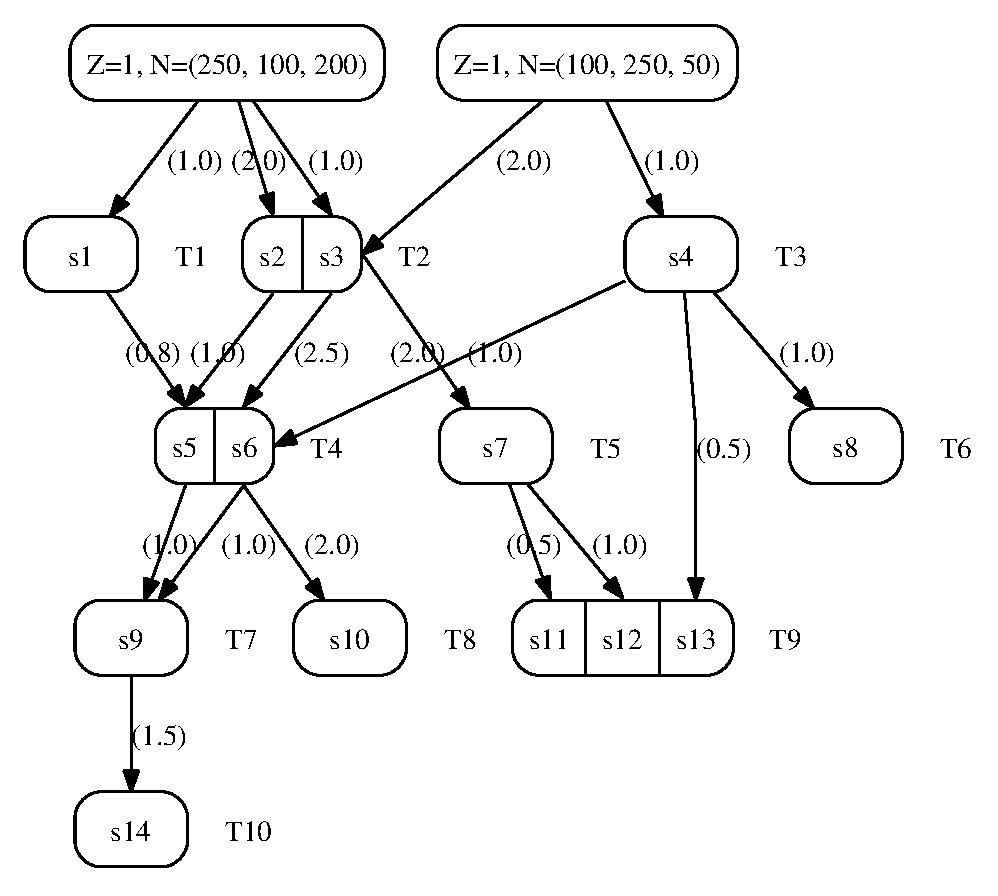
\includegraphics[scale=0.75]{image/example1services}
%\caption[An example small scale service center]{Represents an example small scale service center: the call graph of services and classes $y$, the  think times $Z$ and number of users $N$ of each class over time, the number of calls from classes to services and the invocation numbers within services $con$. }
%\label{fig:service_call_graph}
%\end{center}
%\end{figure}
%
%The class-to-service adjacency matrix obtained through the equations \ref{eq: compute-adjacency-matrix} from adjacency matrix of the service-class call graph is as follows: 
%\[
 %Y=\left(\begin{array}{cccccccccccccc} 1 & 2 & 1 & 0 & 2.8 & 2.5 & 1 & 0 & 5.3 & 5 & 0.5 & 1 & 0 & 7.95\\ 0 & 0 & 2 & 1 & 0 & 7 & 2 & 1 & 7 & 14 & 1 & 2 & 0.5 & 10.5 \end{array}\right)
%\]
%
%There are 6 available hosts to support the services. Capacity of the hosts are as  $\capp=[16\ 6\ 6\ 16\ 6\ 6]^T$ and their CPU speed factor is $\speedFactor=[1\ 1.2\ 0.9\ 1.1\ 0.8\ 1.2]$. The infrastructure cost coefficient was considered %roughly equal for all hosts except 
%a  random component that was added to break the symmetry and make the solution sparse: 
%$ \text{cost}=\text{rand}(H,T) $. 
%
%\newcounter{example}
%\addtocounter{example}{1}
  %\subsection{Example \arabic{example}: A Comparison of the Optimal Control and the Step-by-Step Optimization, a Hypothetical Case of a Fully Known Workload}      
 %In this simple example, we show the effect of solving a service placement problem through the optimal control framework. We show that if an objective is to avoid reconfiguration, and the workload has oscillations, the optimal control provides better results than the step-vise optimization.
 %
 %In order to make it simpler to understand, in this example, we make some unrealistic assumptions. We assume the service center has a very short lifetime of three time steps: $T=4$. The workload for this example was considered to be: 
%\[
%N=\left(\begin{array}{cccc} 0 & 220.0 & 150.0 & 200.0\\ 0 & 100.0 & 170.0 & 110.0 \end{array}\right)
%\]
  %Here, because of the limited number of timestamps, we need to make the assumption of fully knowing the workload for the whole simulation interval. In the next examples, however, we show for the optimal control approach to work, there is no need for knowledge or prediction of future workload.  The only assumptions is that at any given interval the workload has a  mean value.  % and this mean value tends to move slowly. 
   %
 %The response time SLA for all the steps were set to:  $R^\text{SLA}_t = [0.146 \  0.267]^T$. Based on the equation \ref{eq:convert-response-time-SLA-throughput} the optimizer substitutes $R_{SLA}$ and $N$ by:    
%\[
  %X_{SLA}=
%\left(\begin{array}{cccc} 0 & 192.0 & 130.9 & 174.5\\ 0 & 78.93 & 134.2 & 86.82 \end{array}\right) 
%\] 
%
 %The optimization was applied in two settings: with and without a relocation cost. Solving the overall optimization problem with a zero relocation cost, gives the same answer as solving a set of individual optimizations for separate steps.           
 %In other words, the optimizer acts in a fully reactive mode, doing its best to obey the SLA at each step.   
 %In the second case, the relocation cost is taken into account and the optimizer tries to satisfy the SLAs while minimizing the total number of relocations \footnote{In fact the controller tries to minimize the amount of resource adjustment to the services replicas, but this, in most cases means minimizing the number of replica relocations.  }. 
 %Also, note that in both cases the hosts are initially empty and no replica is deployed on them: $\theta_{s,h,0} = 0 \text{   for all $s$,$h$.}$. 
%
  %%  \subsubsection{Overall Optimization} 
 %In the overall optimization case, the optimizer achieves the desired throughput by an initial deployment of 19 service replicas in the first step and a total addition of 0 and removal of 0 in the subsequent steps (total changes of 19). 
%The placement at each step is demonstrated in Figure \ref{fig:overal_optimal_example}. It represents the placement decision at t=0. %
%%
%%
%\begin{figure}[htbp]\begin{center}\subfloat[Overall optimal
%example][Initial placement decision (decision at
%$t=1$)]{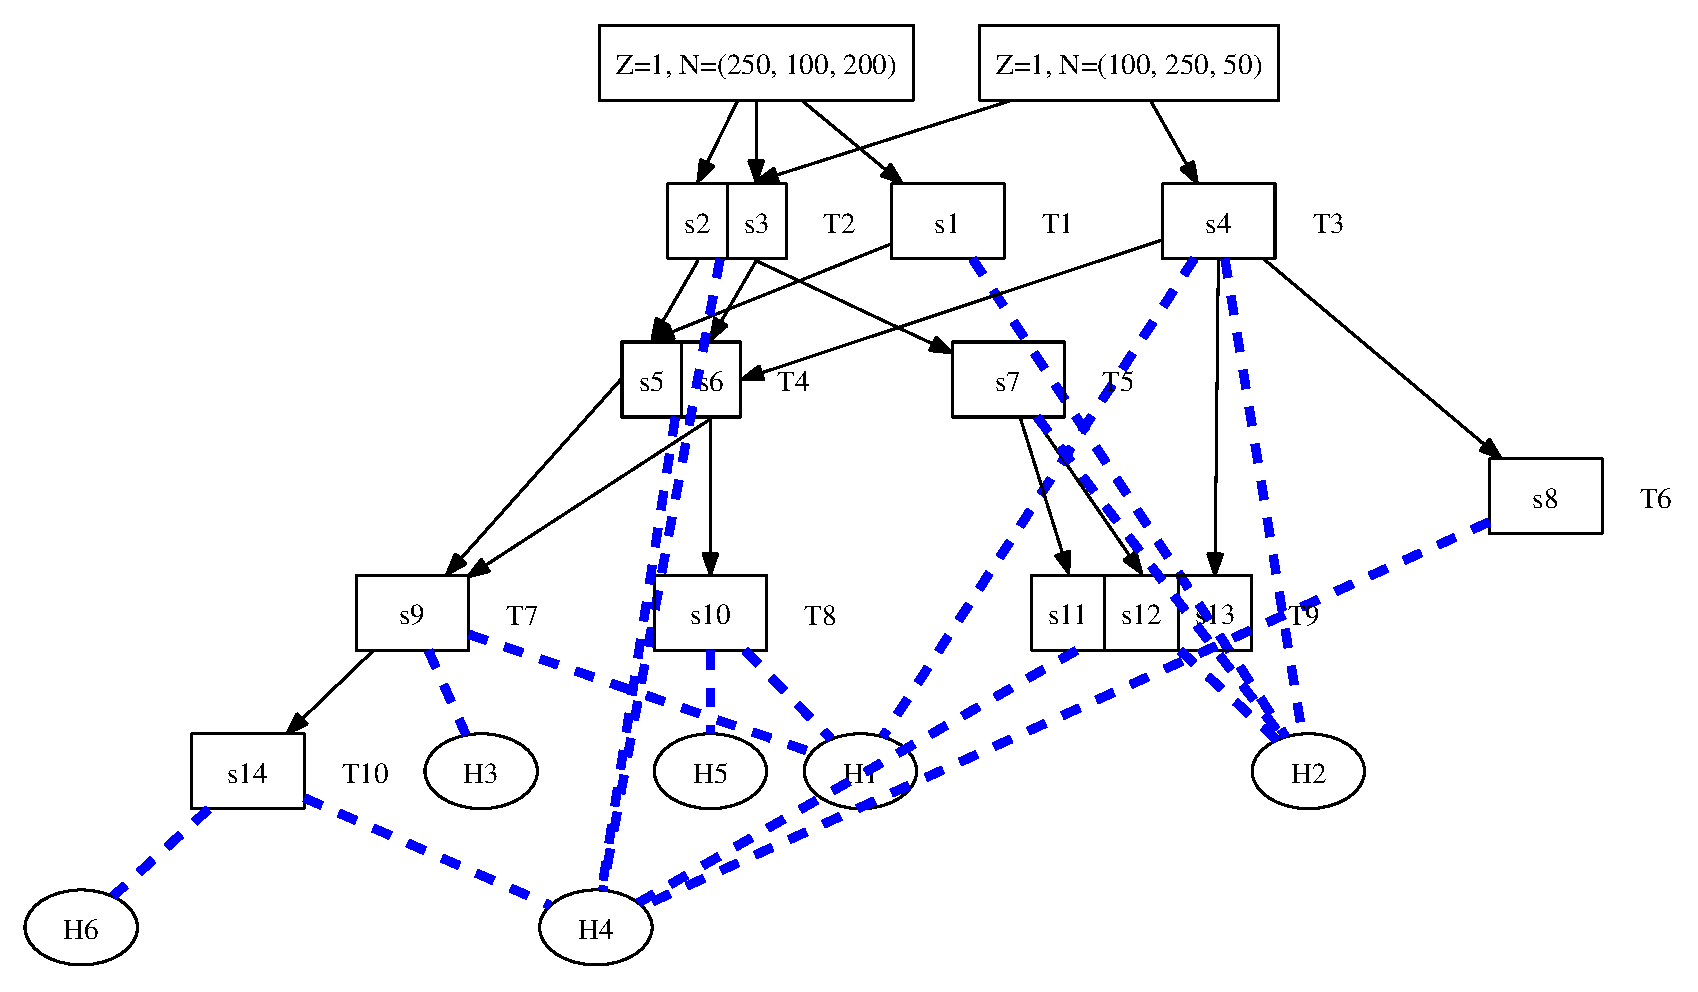
\includegraphics[scale=0.4]{image/example1deployment_overal_step1}
%\label{fig:subfig1}}
% [Represents the placement decisions for a small service center
%using the optimal control.]{Represents the placement decisions for a
%small service center using the optimal control.
%}\label{fig:overal_optimal_example}\end{center}\end{figure}%
%%
%% The (un)deployments are follows: 
%%
%%\begin{spacing}{1} 
%%
%%\begin{eqnarray*} 
%%
%%\begin{split}
%%
%%\text{t=2:} \\
%%
%%& 8   &  \text{added to }  & 2\\
%%
%%& 8  &   \text{added to } & 4 \\
%%
%%\text{t=3:}  \\
%%
%% &  3   &  \text{remove from } & 1 \\
%%
%%&   7  &    \text{added to } & 4 \\
%%
%% &   8  &    \text{remove from } & 4 \\
%%
%%\end{split}
%%
%%\end{eqnarray*}  
%%
%%\end{spacing}
%%
%%  
%%
%%
%%
%% At $t=2$ the container T8 is added to the hosts H2 and H4. this is because an increase in the class C2 population stresses the service $s10$. as  the workload of the second class decreases at $t=3$, containers T3 and T8 are removed from the hosts H1 and H4, and a replica of container T7 is added to the host H4. Note that the services on container T7 are mainly used by class C1. Also, see how service T8 is deployed on host H4 at $t=2$ but it is again removed from it in the next step,  $t=3$.
%%
%
 %% \subsubsection{Step-by-Step Optimization Ignoring the Relocation Cost}  
 %In the step-by-step optimization, where the relocation cost is ignored, the optimizer achieves the desired throughput by an initial deployment of 18 replicas in the first step and a total addition of 9 and removal of 11 in the subsequent steps (total changes of 38). The placements are depicted in Figure \ref{fig:stage_based_optimal_example}. 
%The undirected blue dashed lines denote the placements that have been added in the corresponding steps and the red dashed lines represent the placements that have been just removed at each time step. The black dashed lines denote the placements that performed in the past time step.
%
%\begin{figure}[htbp]
%\begin{center}
%\subfloat[Overall optimal example][Initial placement decision (decision at $t=1$)]{ 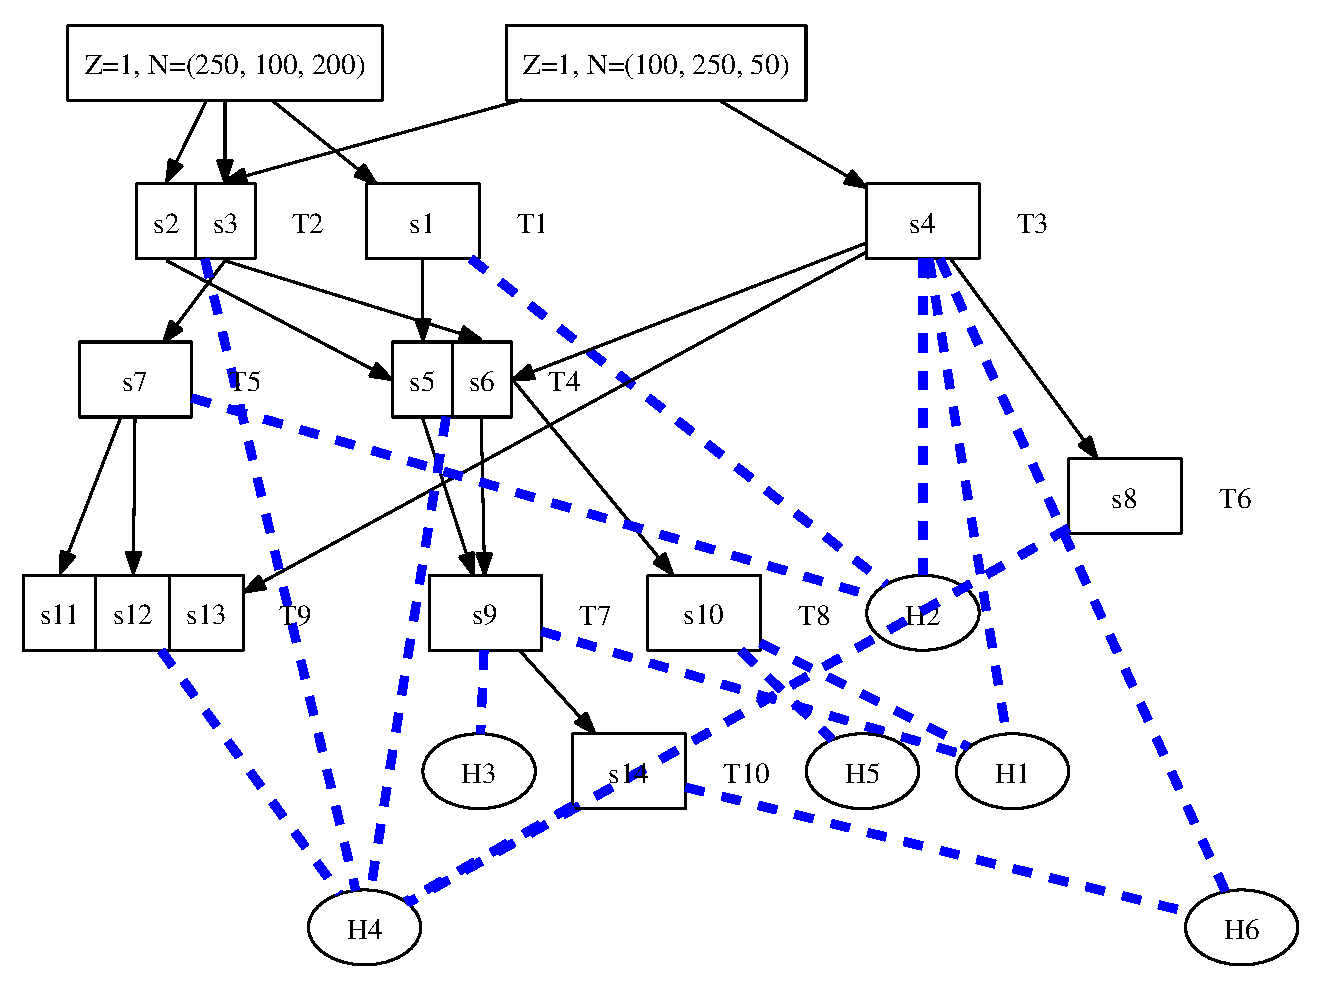
\includegraphics[scale=0.35]{image/example1deployment_step1} \label{fig:subfig1}}  
 %\qquad  
%%
%\subfloat[Subfigure 1 list of figures text][Placement decision at $t=2$]{
 %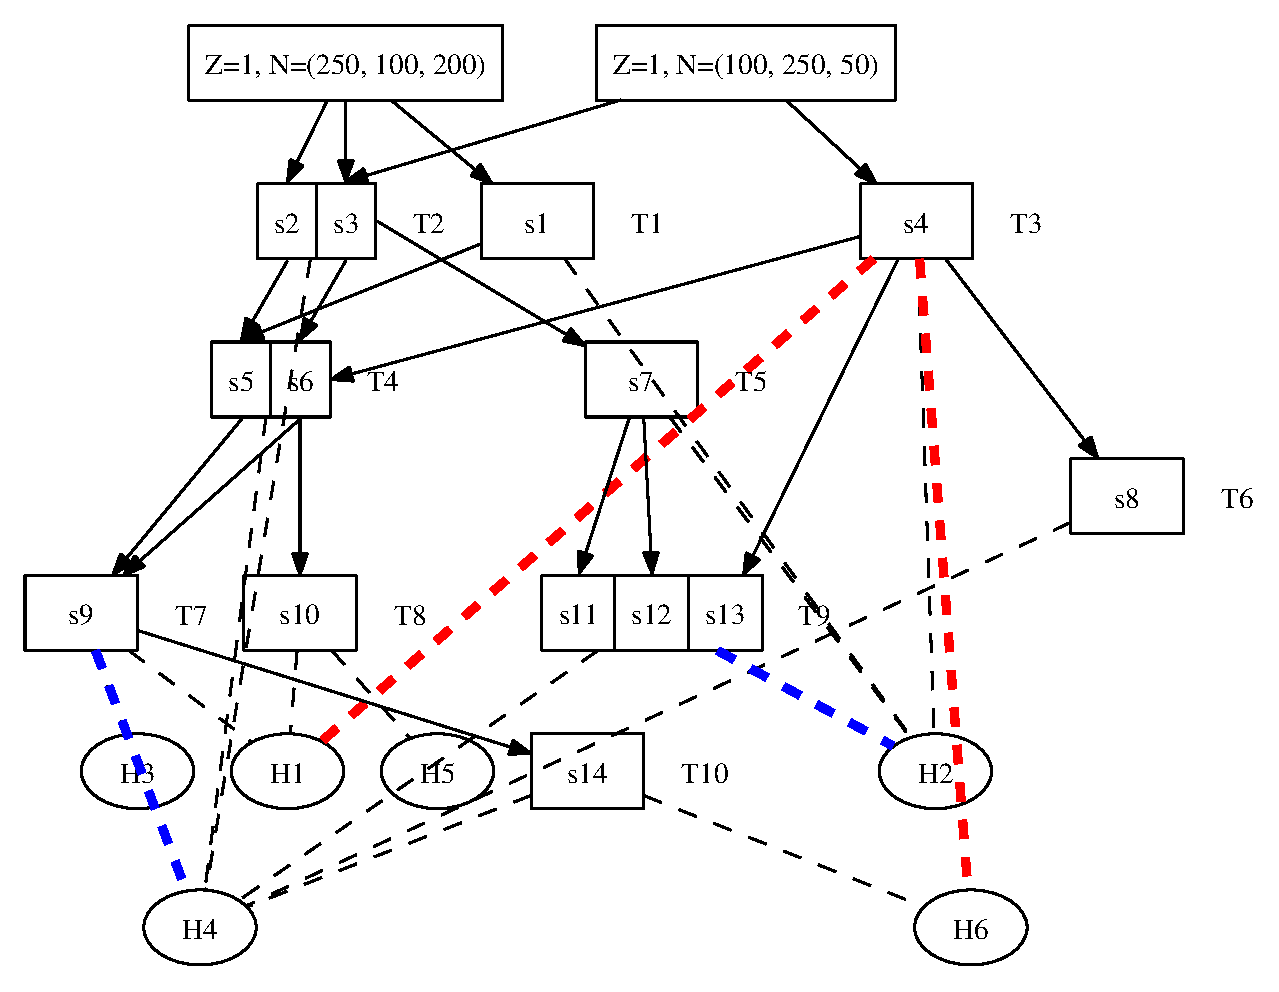
\includegraphics[scale=0.35]{image/example1deployment_step2} \label{fig:subfig2}} 
  %\qquad
%%
  %\subfloat[Subfigure 1 list of figures text][Placement decision at $t=3$]{
 %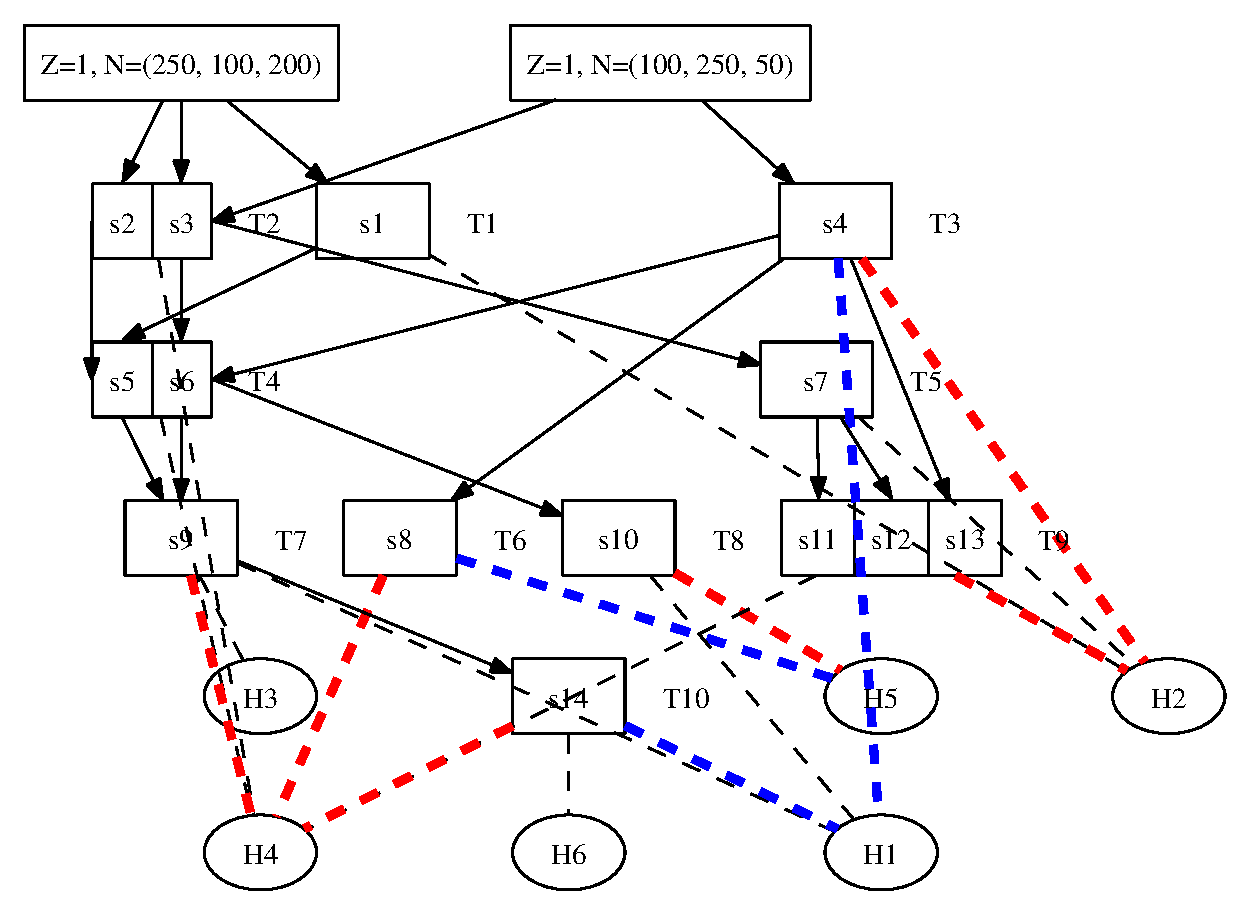
\includegraphics[scale=0.35]{image/example1deployment_step3} \label{fig:subfig3}} 
 %%
%\caption[An example of placement decisions for a small service center using step based optimization, ignoring the future steps.]{An example of placement decisions for a small service center using step based optimization, ignoring future steps.}
%\label{fig:stage_based_optimal_example}  
%\end{center}
%\end{figure}  
%
%and the (un)deployments are as follows:
%\begin{spacing}{1} 
%\begin{eqnarray*}
%\begin{split}
%\text{t=2:} \\
%& 4   &  \text{removed from }  &  4\\ 
%& 5   &  \text{removed from }  &  2\\ 
%& 5   &  \text{added to }  &  3\\ 
%& 9   &  \text{added to }  &  2\\ 
%& 10   &  \text{added to }  &  4\\ 
%& 14   &  \text{added to }  &  3\\ 
%& 14   &  \text{removed from }  &  6\\ 
%\text{t=3:} \\
%& 2   &  \text{removed from }  &  3\\ 
%& 2   &  \text{added to }  &  4\\ 
%& 4   &  \text{added to }  &  4\\ 
%& 4   &  \text{removed from }  &  5\\ 
%& 5   &  \text{added to }  &  2\\ 
%& 5   &  \text{removed from }  &  3\\ 
%& 8   &  \text{added to }  &  1\\ 
%& 8   &  \text{removed from }  &  5\\ 
%& 9   &  \text{removed from }  &  2\\ 
%& 10   &  \text{removed from }  &  4\\ 
%& 14   &  \text{removed from }  &  3\\ 
%& 14   &  \text{removed from }  &  5\\ 
%& 14   &  \text{added to }  &  6\\ 
%\end{split}
%\end{eqnarray*} 
%\end{spacing} 
%
%% note how services 6 and 10 are migrated in the same step.
 %These migrations increase the overall cost in the original objective function and make this solution suboptimal.
 %This clearly shows that when the cost of reconfiguration neglected,
%the overall optimality cannot be achieved in terms of original objectives (although optimization can be distributed over time steps). 
  %
%\addtocounter{example}{1}
 %\subsection{Example \arabic{example}: The Controller Reaction to Adding a Service} 
%In this example, we show how the controller responds to arrival of a new class of users. 
  %Consider the same small size service center.  In this example we assume that the system is already stabilized to the $N_{c1}=160$ users of class $c1$ with response time goal of $R^\text{SLA}_{c1}=0.146$. The class c2 joins the system at $t=1$ with a population of $N_{c2}=100$ and a SLA of $R^\text{SLA}_{c2}=1.146$. The controller uses a quadratic stage cost function for reconfiguration. We performed a simulation of $T=100$ steps that captures the behaviour of a controlled service center until it converges to a steady-state value.   
  %
 %Figure \ref{fig:adding_class_host_portion} represents the response of the system in terms of the utilization of the hosts. Since most of the services for the class $c2$ are hosted on hosts h1 and h2, we see an increase in their utilization. The decreasing utilization of h3 and h4 is due to the departure of the service replicas from them.  
 %Figure \ref{fig:adding_class_serv_portion} shows the amount of resource given to each service, which is increased for all of the services after the 2nd class is added to the system. 
 %Figure \ref{fig:adding_class_throughput} presents the throughput of the classes. 
  %As noted  it takes around 7 steps for the throughput of the class c2 to reach its SLA value. The duration of this convergence depends on the reconfiguration cost coefficient which has been set it to $r_3=100$.  
    %
%\begin{figure}
%\begin{center}
%\subfloat[Service addition scenario, response of the system in terms of utilization of the hosts.][Utilization of the hosts over time.]{
 %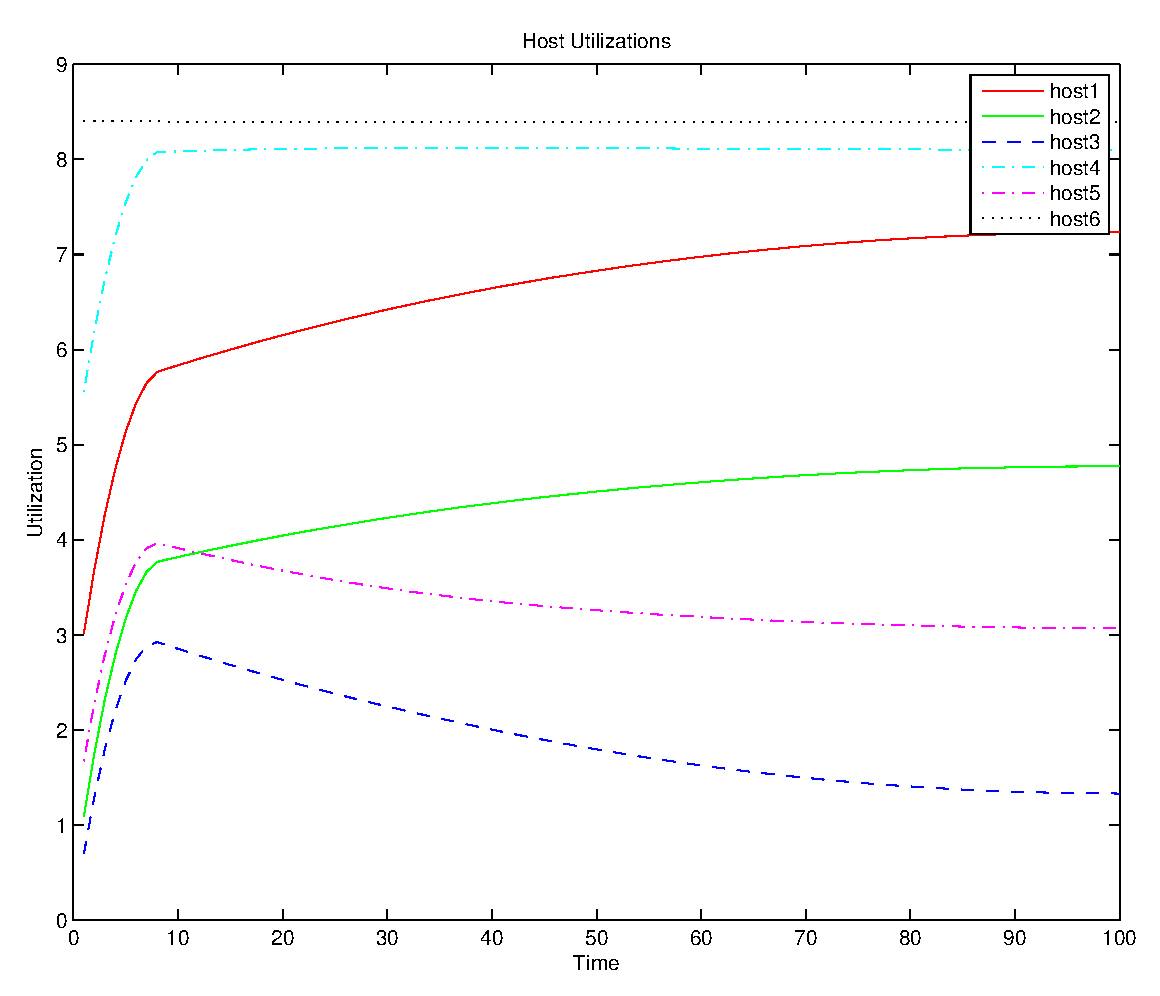
\includegraphics[scale=0.4]{image/placement/adding_class_host_portion} \label{fig:adding_class_host_portion}} 
%\subfloat[Service addition scenario, amount of resource given to each service][Amount of resource given to each service]{
 %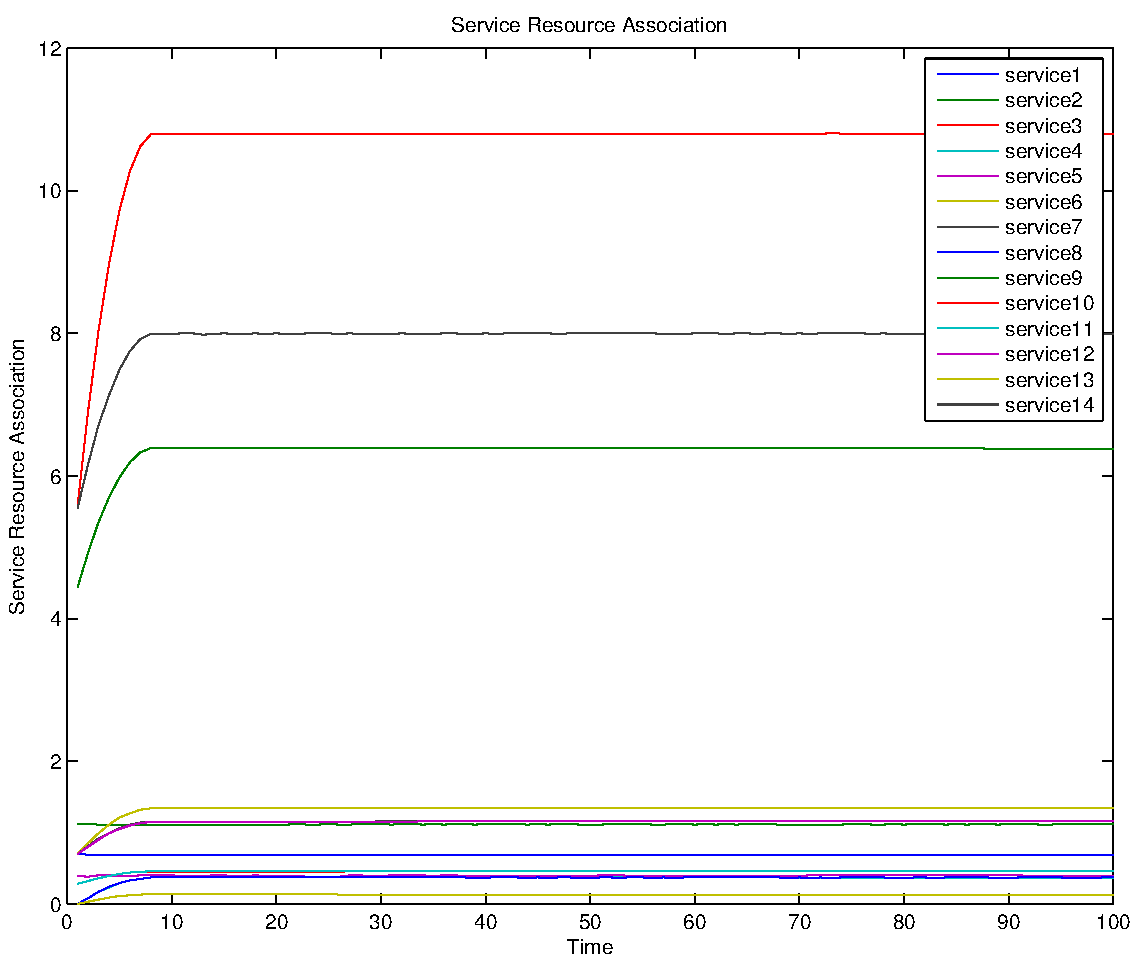
\includegraphics[scale=0.4]{image/placement/adding_class_serv_portion} \label{fig:adding_class_serv_portion}} 
  %\qquad
  %\subfloat[Service addition scenario, the throughput of classes][ the throughput of classes]{
 %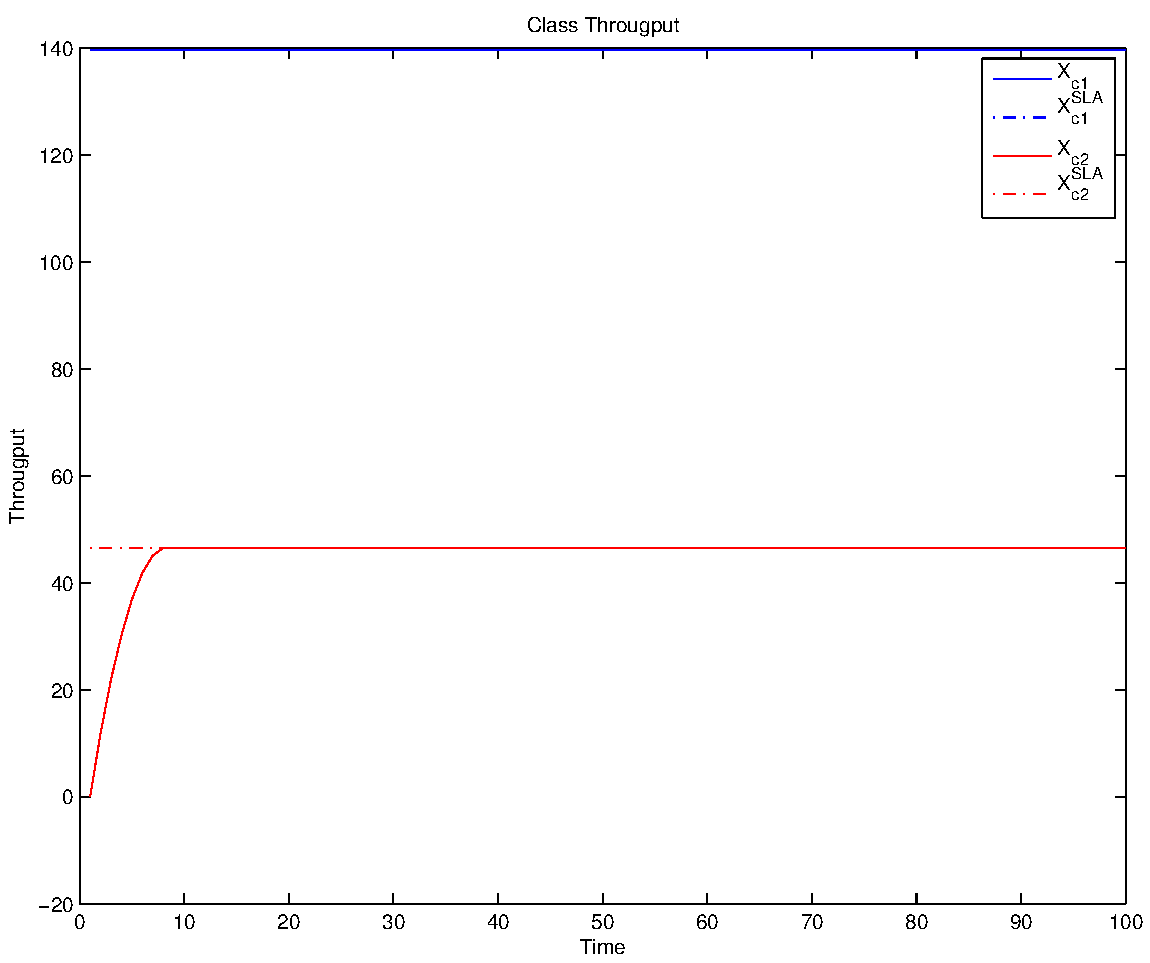
\includegraphics[scale=0.4]{image/placement/adding_class_throughput} \label{fig:adding_class_throughput}} 
 %\subfloat[Service addition scenario, ][resource share of service replicas]{
 %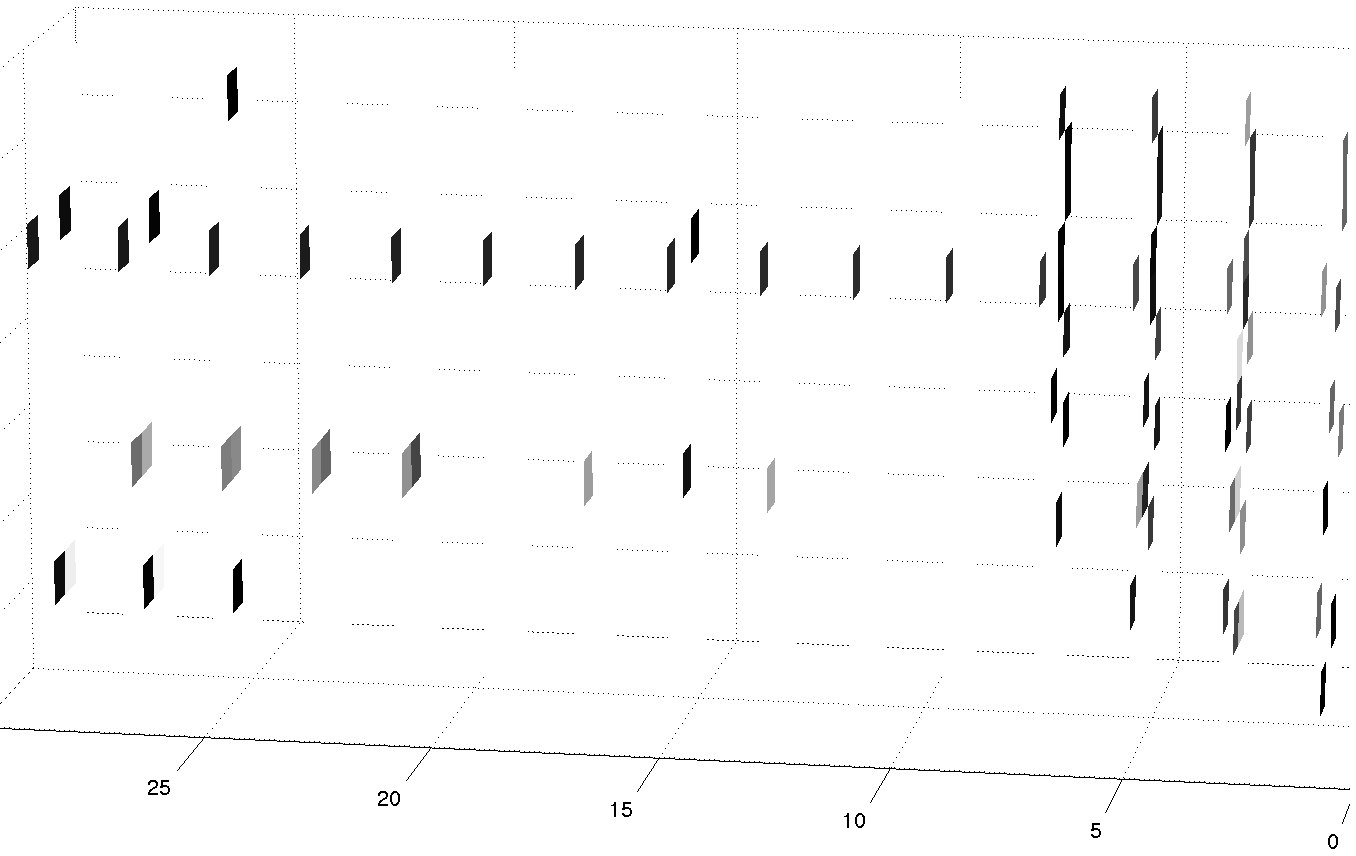
\includegraphics[scale=0.35]{image/placement/adding_class_theta} \label{fig:adding_class_theta}}    
%\caption[Placement controller response to arrival  of a new class  of users]{Placement controller response to arrival  of a new class  of users. }
%\label{fig:stage_based_optimal_example}  
%\end{center}
%\end{figure}
      %Figure \ref{fig:adding_class_theta}    represents the service replicas whose resource share is affected more than 12\% of their original resource share.  Each square represents a  service replica at a certain time t.  The color intensity of the square represents the percentage of resource associated with the service  replica relative to its maximum during its lifetime. 
         %
      %\addtocounter{example}{1}
  %\subsection{Example \arabic{example}: Controller Reaction to Changing Cost Coefficient} 
   %In this example is shown how the distribution of service replicas can be changed using the change in placement coefficient, say from $c_1$ to $c_2$;  and how this transition is controlled by the controller over time in a way that it introduces minimal reconfiguration cost. A simulation is done over T=100 steps. 
  %
  %The workload and SLA of the system is assumed constant, $N=[160 100]'$, $Z=[1  1]'$, $RT_sla=[0.146  1.146 ]'$  during the experiment. 
   %The coefficients are assumed to be H-by-S matrix containing pseudorandom values drawn from the standard uniform distribution on the open interval (0,1) ($c_1=rand(H,S)$, $c_2=rand(H,S)$). 
 %The controller is initially assumed to have been driven by the workload, SLA, and placement coefficient $c_1$ and now in a stable state. 
  %At time $t=1$ the coefficient $c_2$ is suddenly  given to the controller to be applied.  
%\begin{figure} 
%\begin{center}
%\subfloat[Cost coefficient change scenario,  allocation of resources service replicas.][ Allocation of resources to service replicas. ]{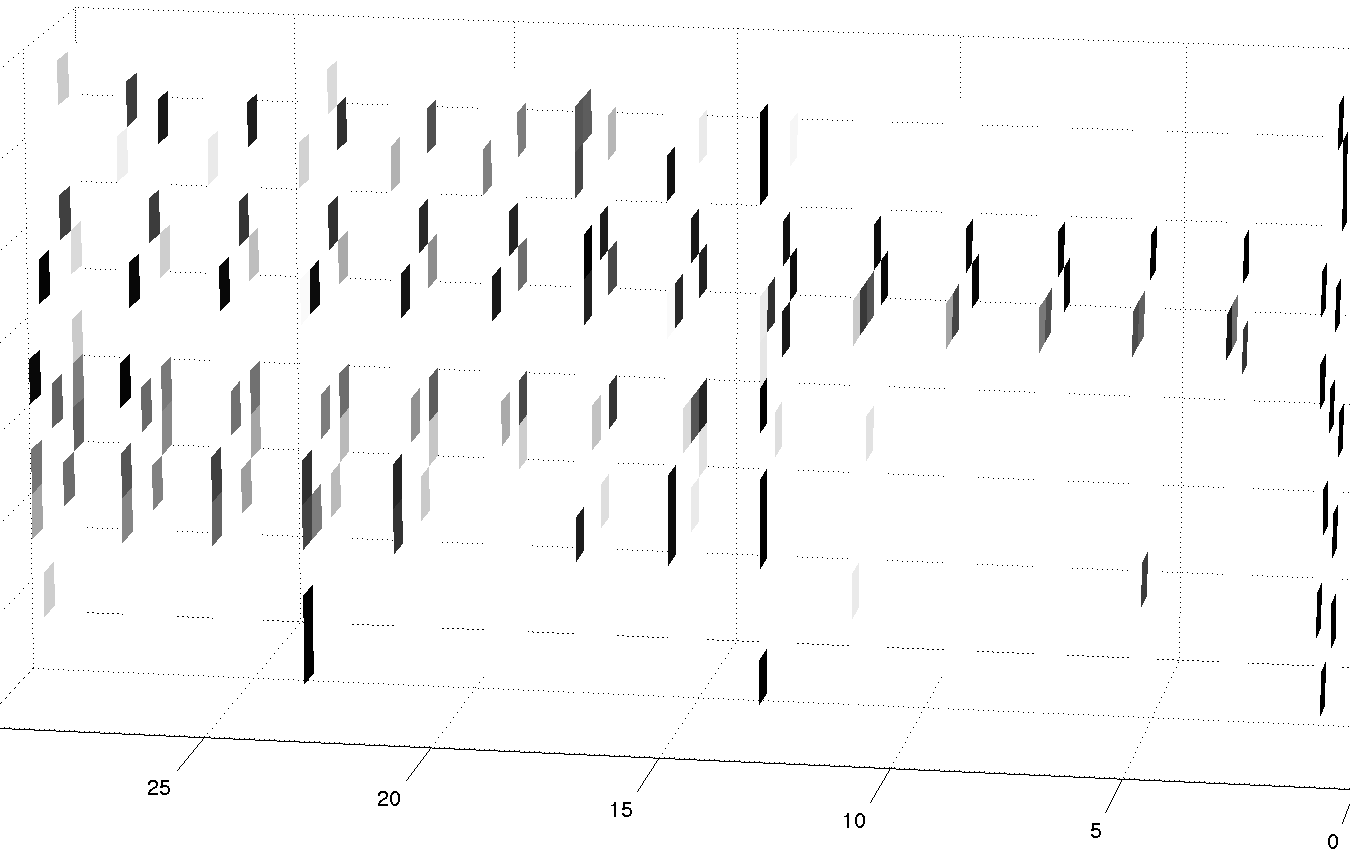
\includegraphics[scale=0.35]{image/placement/test_change_cost_coef_theta_matrix} \label{fig:test_change_cost_coef_theta_matrix}} 
 %%
  %\subfloat[Cost coefficient change scenario, utilization of hosts.][Utilization of hosts.] {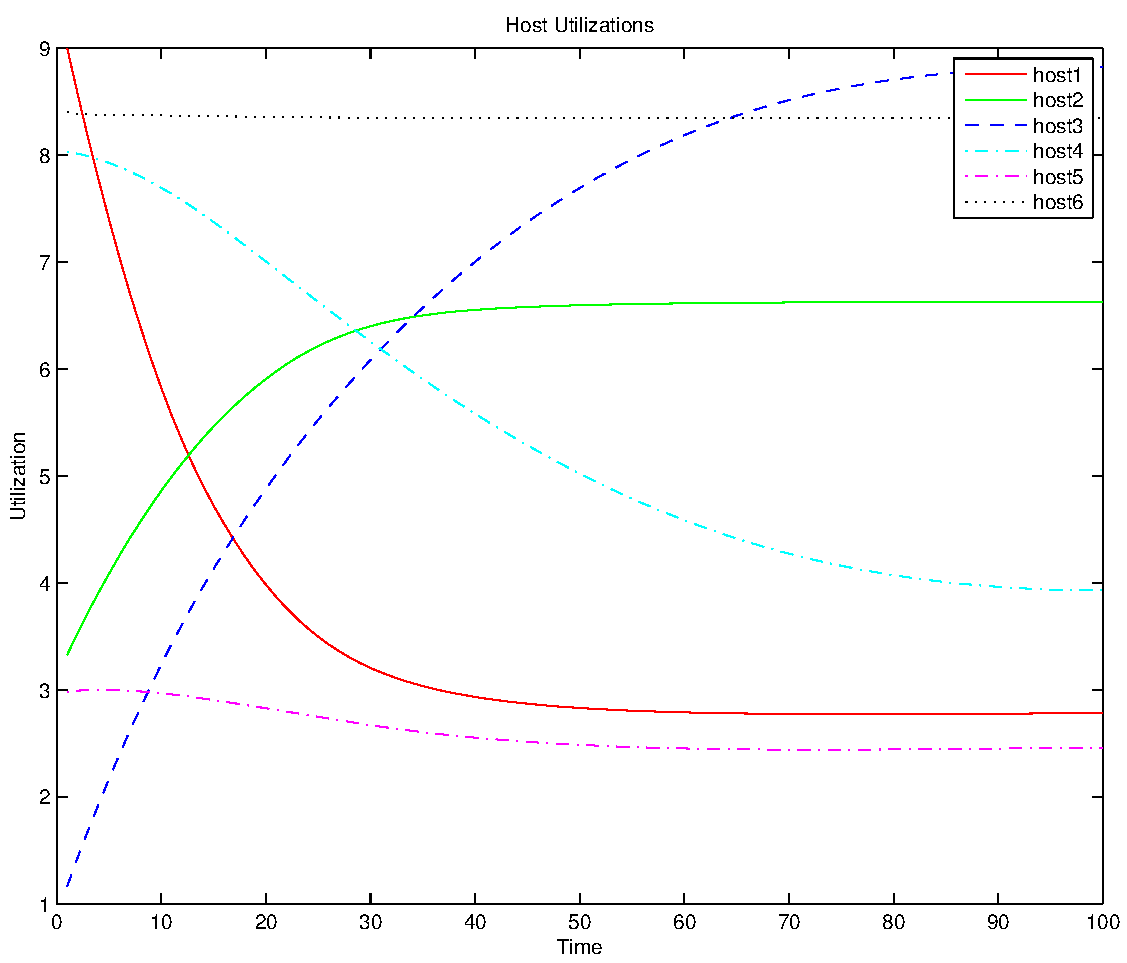
\includegraphics[scale=0.4]{image/placement/test_change_cost_coef_util} \label{fig:test_change_cost_coef_util}} 
%%
   %\qquad
  %\subfloat[Cost coefficient change scenario, stabilized placement at the beginning (red) and end (blue) of control interval. ][Stabilized placement at the beginning (red) and end (blue) of control interval.]{\includegraphics[scale=0.5]{image/placement/test_change_cost_coef_static} \label{fig:test_change_cost_coef_static}}   
  %%
   %\subfloat[Cost coefficient change scenario, service allocation of service replicas.][Service allocation of service replicas.]{\includegraphics[scale=0.4]{image/placement/test_change_cost_coef_theta}    \label{fig:test_change_cost_coef_theta}}    
%\caption[Placement controller response to change in the cost coefficient.] {Placement controller response to change in the cost coefficient. } 
%\label{fig:cost-coefficient-change-scenario}  
%\end{center}
%\end{figure}
 %Figure \ref{fig:test_change_cost_coef_static}  represents the stabilized placement at the beginning  and end of control interval ( denoted by blue and  red markers  consecutively).  
  %Figure \ref{fig:test_change_cost_coef_theta}  represents the change of  allocated resource to service replicas during the control interval.  
   %Figure \ref{fig:test_change_cost_coef_util}  represents the utilization of the hosts over the control interval.  
%
 %\addtocounter{example}{1}
 %\subsection{Example \arabic{example}: The Controller Reaction to a Change in the SLAs }     
     %In this example, we show how the controller reacts to the changes in the response time SLAs. The workload and the optimization parameters, for the duration of this simulation, are constant and are as follows: $r=[5\ 1\ 100]$, $N=[160\ 100]^T$, $Z=[1\ 1]^T$, $c=rand(H,S)$. Between times $t=1$ and $t=100$ the response time SLA is as follows: $RT^\text{SLA}(t)=[0.46\  1.146 ]^T$. Between times $t=101$ and $t=200$ the response time SLA is as follows:  $RT^\text{SLA}(t)=[0.146\  1.146 ]^T$. The controller increases the amount of resource given to the service replicas in order to accommodate the more demanding SLA after t=100.   
    %
    %There is a small difference between this example  and the examples usually used in conventional  PID control;  instead of feeding the $RT^\text{SLA}(t)$ signal to the controller one step at a time, it is given to the controller in advance.  In other words we ask the controller to get the response time to the desired value at time step $T$. As a result,  using MPC becomes inevitable.  
  %\begin{figure}
%\begin{center}  
%\subfloat[The increase in the utilization of te hosts when the controller adjusts to a tighter SLA.][Increase in the utilization of the hosts when the controller adjusts to a tighter SLA.]{\includegraphics[scale=0.4]{image/placement/sla_change_host_portion} \label{fig:sla_change_host_portion}}
%%
%\subfloat[ Increase in the amount of resource  given to service replicas.][ Increase in the amount of resource  given to service replicas.]{\includegraphics[scale=0.4]{image/placement/sla_change_theta}\label{fig:sla_change_theta}} 
  %\qquad
 %%   
%\subfloat[ Changes in the response time of class $c_1$ based on the given response time SLA.][Changes in the response time of class $c_1$ based on the given response time SLA.]{\includegraphics[scale=0.4]{image/placement/sla_change_rt} \label{fig:sla_change_rt} } 
  %\end{center}
%\end{figure}
%Figure \ref{fig:sla_change_theta}  shows how the services that are bottleneck are provisioned using more resources for their replicas in order to increase the throughput of the  associated class and improve its response time. Since services $s_{10}$ and $s_{14}$ are the major bottleneck for the class $c_1$ (whose response time SLA has decreased), the controller increases their portion of resources on hosts $h_6$ and $h_2$ respectively. 
     %Figure \ref{fig:sla_change_host_portion}  represents the change in the utilization of hosts when the controller adjusts to a tighter SLA. Figure \ref{fig:sla_change_rt} represents how the response time of class $c_1$ is driven to the specified SLA by a specified time.
    %
  %
 %\addtocounter{example}{1}         
 %\subsection{Example \arabic{example}: The Controller Response to a Dynamic Workload }   
   %In this example, we show how the controller reacts to a dynamic workload. 
 %Unlike the examples 1 to 6, that the input parameters to the system  (Workload, SLA, etc) change with a step like function pattern, in order to show the reaction of the controller, in this example we assume that the workload changes over time with a sinus like pattern. This is to investigate the response of the controller to a workload that introduces some thrashing.     
  %Figure \ref{fig:dynamic_workload} represents the workload.   
  %
   %In this example we set a relatively high cost coefficient value for the SLA violation cost ($r_\text{SLA}=50$  compared to $r_\text{resource}=1$). So the main trade-off is between the infrastructure and the reconfiguration costs.  
 %
  %\begin{figure}
%\begin{center}  
  %\subfloat[A sinus like workload][A sinus like workload] {\includegraphics[scale=0.2]{image/placement/dynamic_workload.eps}\label{fig:dynamic_workload}  }  
  %\hspace{0.4cm}
  %%
%\subfloat[The cost of resource and the cost of reconfiguration for (optimal, MPC, no-reconfiguration-cost) placement controllers with parameters $T=7$ and $r_\text{trsh}=40$ and first norm reconfiguration cost function to a sinus like workload.][Resource cost and reconfiguration cost for the 1st norm penalty parameters $T=7$ and $r_\text{trsh}=40$.]{\includegraphics[scale=0.2]{image/placement/dynamic_infrastructure_cost_nsteps50_T7_rTRSH40abs.eps}
  %\includegraphics[scale=0.2]{image/placement/dynamic_trashing_cost_nsteps50_T7_rTRSH40abs.eps}
  %\label{fig:dynamic_cost_nsteps50_T7_rTRSH40abs}}  
 %\qquad
 %%
%\subfloat[The cost of resource  and cost of reconfiguration for (optimal, MPC, and no-reconfiguration-cost) placement controllers with parameters $T=7$ and $r_\text{trsh}=100$  and first norm  reconfiguration cost function to a sinus like workload.][Resource and reconfiguration cost for 1st norm penalty, and parameters $T=7$ and $r_\text{trsh}=100$.] {\includegraphics[scale=0.2]{image/placement/dynamic_infrastructure_cost_nsteps50_T7_rTRSH100abs.eps}
  %\includegraphics[scale=0.2]{image/placement/dynamic_trashing_cost_nsteps50_T7_rTRSH100abs.eps}
  %\label{fig:dynamic_cost_nsteps50_T7_rTRSH100abs}}   % \hspace{0.2cm}
  %%
 %\subfloat[The cost of resource  and cost of reconfiguration for (optimal, MPC, and zero-reconfiguration-cost) placement controllers  with parameters $T=7$ and $r_\text{trsh}=400$  and first norm  reconfiguration cost function to a sinus like workload][Resource and reconfiguration cost for 1st norm penalty, and parameters $T=7$ and $r_\text{trsh}=400$.] {\includegraphics[scale=0.2]{image/placement/dynamic_infrastructure_cost_nsteps50_T7_rTRSH400abs.eps}
%\includegraphics[scale=0.2]{image/placement/dynamic_trashing_cost_nsteps50_T7_rTRSH400abs.eps}
%\label{fig:dynamic_cost_nsteps50_T7_rTRSH400abs}}
%\qquad
%\subfloat[The cost of resource  and cost of reconfiguration for (optimal, MPC, and zero-reconfiguration-cost) placement controllers  with parameters $T=7$ and $r_\text{trsh}=400$  and second norm reconfiguration cost function  to a sinus like workload][Resource and reconfiguration cost for  2nd norm penalty, and parameters $T=7$ and $r_\text{trsh}=400$. ] {\includegraphics[scale=0.2]{image/placement/dynamic_infrastructure_cost_nsteps50_T7_rTRSH400square.eps}
%\includegraphics[scale=0.2]{image/placement/dynamic_trashing_cost_nsteps50_T7_rTRSH400square}
%\label{fig:dynamic_cost_nsteps50_T7_rTRSH400square}}  % \hspace{0.2cm}
%%
%\subfloat[The cost of resource  and cost of reconfiguration for (optimal, MPC, and zero-reconfiguration-cost) placement controllers  with parameters $T=7$ and $r_\text{trsh}=400$  and second norm reconfiguration cost function  to a sinus like workload. ][Resource and reconfiguration cost for 2nd norm penalty, and parameters $T=7$ and $r_\text{trsh}=4000$. ] {\includegraphics[scale=0.2]{image/placement/dynamic_infrastructure_cost_nsteps50_T7_rTRSH4000square.eps}
%\includegraphics[scale=0.2]{image/placement/dynamic_trashing_cost_nsteps50_T7_rTRSH4000square}
%\label{fig:dynamic_cost_nsteps50_T7_rTRSH4000square}}
%%
%%
%\label{fig:cost-coefficient-change-scenario}  
%\end{center}
%\end{figure}
%
 %Figure \ref{fig:dynamic_cost_nsteps50_T7_rTRSH40abs} presents the cost of resource and the cost of reconfiguration for an optimal, MPC, no-reconfiguration-cost placement controllers when this workload is applied. The blue line in the figure represents the cost for the zero-reconfiguration-cost controller, a controller that has 0 reconfiguration cost coefficient and thus ignores the reconfiguration cost. The redline belongs to the optimal controller where it solves the optimal control problem for the whole interval assuming that the workload is known.  The green line represents the MPC controller. The MPC controller in this example uses the first norm function for the reconfiguration cost and has the parameter values of $T=7$ and $r_\text{trsh}=40$.  In figures \ref{fig:dynamic_cost_nsteps50_T7_rTRSH100abs} and 
   %\ref{fig:dynamic_cost_nsteps50_T7_rTRSH400abs}, we increase  the reconfiguration cost coefficient to 100 and 400 respectively. At $r_\text{trsh}=100$ we can see that the MPC controller completely gave up on adjusting to the decreasing workload but the optimal control still does some adjustment in response to the decrease.   
 %
 %When the reconfiguration's stage cost is defined using the first norm, the controller  `choice' between objectives becomes clear-cut. Unlike the second norm, where the controller compromises between the reconfiguration, preserving the SLAs, and infrastructure cost at every single timestep, a first norm stage cost controller makes  a clear decision on what objective to follow. As a result we see the controller is sometimes completely giving up the reconfiguration objective on workload ups and downs within the lookahead window (e.g. MPC controller in Figure \ref{fig:dynamic_cost_nsteps50_T7_rTRSH40abs}), sometimes giving up on saving infrastructure cost when workload decreases (Figure \ref{fig:dynamic_cost_nsteps50_T7_rTRSH100abs}), or the SLA violation cost when the workload increases. Essentially, with the first norm if the controller detects a change in the state of the system  (i.e. SLA, workload, or placement coefficients), it will either react to it immediately  or just ignores it.  
 %This decision is based on its prediction of change within the prediction window (e.g. $T=7$), and its behaviour depends heavily on this prediction. If the controller predicts that the change is permanent within the prediction window (i.e. it is not going to be reversed) then it might take immediate action based on the cost. If it detects that the change is temporary, then it most probably ignores doing a modification because of the reconfiguration cost. 
  %Its important however to note that detecting temporary changes in the time window using complicated models  is not necessary, because once the cycles of the workload are detected externally (i.e. by human administrator or a workload analyzer program)  the  cost coefficients and the prediction window of the controller can be updated to reach the desired behaviour  
 %\footnote{In order to change the costs for a specific classes  the cost coefficient scaler values  have to be substituted by vectors,  and there will be it a slight change in the objective function  to make  every  service have a different cost coefficient.}  
    %
  %Figures \ref{fig:dynamic_cost_nsteps50_T7_rTRSH400square} and  \ref{fig:dynamic_cost_nsteps50_T7_rTRSH4000square}  present the cost of resource  and cost of reconfiguration for different placement controllers  constructed with second norm reconfiguration cost function.
 %In \ref{fig:dynamic_cost_nsteps50_T7_rTRSH400square} the reconfiguration cost coefficient is set to $r_\text{trsh}=400$  while in \ref{fig:dynamic_cost_nsteps50_T7_rTRSH4000square}  it is $r_\text{trsh}=4000$.  In both cases and PC is suboptimal but it does a good job matching the optimal. 
%
%
%%   \begin{figure}
%%
%%\begin{center}
%%
%%\subfloat[Reaction of the  controller to the sinus like workload.][Reaction of the  controller to the sinus like workload.]
%%{\includegraphics[scale=0.4]{{image/placement/dynamictest_change_cost_coef_theta_matrix} \label{fig:test_change_cost_coef_theta_matrix}} 
%%   \qquad
%%
%%\end{center}
%%
%%\end{figure}
%%   
 %
%% \addtocounter{example}{1}
%% \subsection{Example \arabic{example}: Controller Response to Stochastic Workload}
  %
  %\section{Work That Remains}      
 %An example should be added in order to show the response of the controller to a stochastic workload. We are going to use two hours of FIFA98 workload to test the controller. A CEC implementation will be utilized where  
 %the mean of the workload parameters, calculated by moving average filters, are going to be used within the CEC controller. %for the whole lookahead window. 
%
  %One example should be added in order to assess the reaction of the controller to adding an unmanaged class.   In a real world, for example, this can be an administrative task run by administrators, or any other operating system process that consumes resources on the hosts. Services of this class are deployed together with managed services into the infrastructure.  The controller should react by moving replicas of the managed services, in a way that it keeps SLA of managed classes satisfied. 
  %% this should represent the response of the controller to addition of an unmanaged class; a class that there is no control over it's placement and resource allocation for its services. 
  %
 %
%% 
%
%%\addtocounter{example}{1}
%% \subsection{Example \arabic{example}: Controller Reaction to Adding an Unmanaged Service}    
%%   In this example we represent the response of the controller to addition of an unmanaged class. There is no control over the placement and resource allocation for services of this class.  In real world, for example, this can be an administrative task run by administrators, or any other operating system process that consumes resources on the hosts.  In terms of modeling, however, the class is modelled by its workload (whose Z, N, D are estimated) and ( hypothetical) services. Services are deployed together with managed services into the infrastructure.  The controller, thus, moves replicas of the managed services around to keep SLA of managed classes satisfied. 
%% 
 %
  %%  Example \arabic{example}:  Controller Response to Stochastic Workload  
  %
  
 \section{Case Study: The Controller Response to a Realistic Workload} 
 \label{sec:cases-study}  
  In this case study, we assess the reaction of the controller to a stochastic workload taken from a real application. The main objective is to test the behaviour of the controller in terms of its ability to navigate the trade-off among SLA violations, resource cost, and the thrashing cost.  The structure of the services, the call graph, and the classes are the same as ones used in the motivating example (section~\ref{sec:motivating-examples}, Figure~\ref{fig:service_call_graph}).
   There are 14 services deployed on 6 hosts, possibly giving 84 service replicas. There are two classes of service utilizing the services.

	The workload for classes is a portion of the well-known FIFA98's workload obtained by processing the Web server logs. We processed the workload of the day 42 of FIFA98 to obtain the number of users for each five-minute interval. This gave 288 samples for the whole day (let us denote these by $N_t$).  We then constructed two 12 hour workloads for two class of users based on this as:
$N_{c1,t}=N_t-200$ for the first 12 hours and $N_{c2,t}= \lfloor N_{t+12h}/2\rfloor-110$ for the second 12 hours. These values are chosen so that the workloads of classes have peaks and valleys to test the controller. 
% Figure \ref{fig:dynamic_workload} presents the workloads in terms of the number of users $N_{c,t}$. 
The think times for the classes are $Z=[1, 1]^T$.
Multiplicity of hosts are $\capp=[9, 10, 10, 9, 10, 7]^T$.
The speed factors for the hosts are $=[1, 1.2, 0.9, 1.1, 0.8, 1.2]^T$
The service demand for the services are $d=[5, 4, 2, 8, 1, 2, 5, 8, 6, 8, 4, 5, 6, 5]\times 10^{-3}$.
The random cost coefficients are $\sigma^*_{s,h}=rand_{H,1}*\textbf{1}_{1,S}+10$.
 Each variable $rand_h$ is a value sampled from random variable of the uniform distribution, $U(0,1)$. 

 The system was simulated using the SimPy \cite{Mueller2003SimPy} simulator. The optimization problem was described using the \texttt{cvx} framework \cite{cvx} in Matlab where the problem is delegated to the SeDuMi \cite{sturm1999using} solver.  

 In this case study we performed two sets of experiments. In the first set, we investigated the effect of different cost coefficients on the behaviour of the controller. In the second set of experiments, we investigate the effect of changing the length of lookahead horizon on the achievable cost trade-offs. 

\subsection{First Set of Experiments: Different Cost Coefficients}
We performed several experiments to test the response of the controller over time.
Here we show the detailed results for two simulations as representatives.
The lookahead horizon for MPC controller is five steps ($J=5$) for both experiments. 
	In the first simulation, we set the cost coefficients as follows: $[\rSLA=50,  \rResource=10, \rDeployment=4]$. 
In the second set, we set cost coefficients to: $[\rSLA=50,  \rResource=1, \rDeployment=40]$. Thus, intuitively the controller in the first configuration cares more about the cost of resources, while in the second configuration it cares more about the cost of reconfiguration. Let us call these controller configurations resource-precedent and reconfiguration-precedent controllers.
The result of simulations is depicted in Figures \ref{fig:case_study_one_relocations}  to \ref{fig:case_study_one_response_time_cdf}.

 \begin{figure}[h]
\centering 
\subfloat[Resource Precedent Controller] {\includegraphics[width=0.5\linewidth]{image/placement/relocations_144steps_7T_50_10_4_abs}\label{fig:relocations_10_4}}
\subfloat[Reconfiguration Precedent Controller] {\includegraphics[width=0.5\linewidth]{image/placement/relocations_144steps_7T_50_1_40_abs}\label{fig:relocations_1_40}}
	\caption{The cumulative distribution function (CDF) of the number of relocations for two different MPC configurations.}
		\label{fig:case_study_one_relocations} 
\end{figure}
Figure \ref{fig:case_study_one_relocations}  represents the cumulative distribution function (CDF) of the number of relocations done for each time step for the resource-precedent controller (\ref{fig:relocations_10_4}) and the reconfiguration-precedent (\ref{fig:relocations_1_40}).
As can be noted, in Figure \ref{fig:relocations_10_4} the $Y$ value of the resource-precedent graph (blue solid line) at 0 jumps to 0.6. This means 60\% of the area under the PDF curve is placed at 0. In other words, in 60\% of steps, there is no relocation. Compared to this, the CDF of the reconfiguration-precedent controller (blue dashed line) shows a lot fewer relocations per step; it has no relocation in almost 82\% of the steps.
%The rest of the steps have 1 to 20 relocations. 
%Only the first step has 70 relocations (not in the diagram), which is why the distribution is long tail. 

\begin{figure}[h]
\centering 
\subfloat[Resource Precedent Controller] {\includegraphics[width=0.5\linewidth]{image/placement/servers_144steps_7T_50_10_4_abs}\label{fig:servers_10_4}}
\subfloat[Reconfiguration Precedent Controller] {\includegraphics[width=0.5\linewidth]{image/placement/servers_144steps_7T_50_1_40_abs}\label{fig:servers_1_40}}
		\caption{The number of active servers over time for two different MPC configurations.}
		\label{fig:case_study_one_number_of_servers}  
\end{figure}
Figure \ref{fig:case_study_one_number_of_servers} represents the number of active servers over time in both configurations.
The figure is consistent with our assumption: the resource-precedent controller (\ref{fig:servers_10_4}) tries to save resources by deactivating/activating physical machines more frequently than the reconfiguration-precedent one (\ref{fig:servers_1_40}).


% has more oscillations. This is because more weight is assigned to the resource costs and less weight to reconfiguration cost; thus, 
%
\begin{figure}
\centering 
\subfloat[Resource Precedent Controller] {\includegraphics[width=0.5\linewidth]{image/placement/rt1_144steps_7T_50_10_4_abs}\label{fig:rt_10_4}}
\subfloat[Reconfiguration Precedent Controller] {\includegraphics[width=0.5\linewidth]{image/placement/rt_144steps_7T_50_1_40_abs}\label{fig:rt_1_40}}
	\caption{The raw response time graphs over time for two different MPC configurations.}
		\label{fig:case_study_one_response_time}
\end{figure}

 To show the extent to which the SLA is satisfied in each scenario, we have provided the raw response time graphs in Figures \ref{fig:rt_10_4} and \ref{fig:rt_1_40}.
\begin{figure}
\subfloat[Resource Precedent Controller] {\includegraphics[width=0.5\linewidth]{image/placement/rtcdf_144steps_7T_50_10_4_abs1}\label{fig:rtcdf_10_4}}
% \subfloat[] {\includegraphics[width=0.5\linewidth]{image/placement/rtcdf_144steps_7T_50_10_4_abs}\label{fig:ts1a}}
\subfloat[Reconfiguration Precedent Controller] {\includegraphics[width=0.5\linewidth]{image/placement/rtcdf_144steps_7T_50_1_40_abs}\label{fig:rtcdf_1_40}}
		\caption{The difference between response time and the response time SLA as a CDF for two different MPC configurations.}
	\label{fig:case_study_one_response_time_cdf}
\end{figure}
 However, it is not very easy to see their difference. In Figures~\ref{fig:rtcdf_10_4} and~\ref{fig:rtcdf_1_40} we represent the difference between the response time and the response time SLA (i.e. $RT_c - RT_c^\text{SLA}$) as a CDF, taking each time step as one sample. 
 %As can be observed, in both scenarios there is no shortage of throughput from the one specified in the SLA.
 In \ref{fig:rtcdf_10_4}, there were some points where the SLA is breached, and that is why the CDF increases into the region $RT_{c}>RT^\text{SLA}_c$. In \ref{fig:rtcdf_1_40}, the response time did not breach the SLA, and the CDF reaches 1 before the region where $RT_{c}>RT^\text{SLA}_c$. 

%
%
%\begin{figure}
%\centering 
%\subfloat[] {\includegraphics[width=0.5\linewidth]{image/placement/util_144steps_7T_50_10_4_abs}\label{fig:ts2a}}
%\subfloat[] {\includegraphics[width=0.5\linewidth]{image/placement/util_144steps_7T_50_1_40_abs}\label{fig:ts2b}}
	%\label{fig:case_study_one_utilization}  
	%\caption{what's up}
%\end{figure}




%\subfloat[] {\includegraphics[width=0.5\linewidth]{image/placement/relocations_144steps_7T_50_1_4_abs}\label{fig:ts1a}}
%\subfloat[] {\includegraphics[width=0.5\linewidth]{image/placement/relocations_144steps_4T_50_1_4_abs}\label{fig:ts1a}}
%\subfloat[] {\includegraphics[width=0.5\linewidth]{image/placement/trade_off_50_1_abs}\label{fig:ts1a}}
%
	  %\subfloat[] {\includegraphics[width=0.5\linewidth]{image/placement/relocations_CDF_compare}\label{fig:ts1a}}
	  %\subfloat[] {\includegraphics[width=0.5\linewidth]{image/placement/active_servers_CDF_compare}\label{fig:ts1b} }
%
				%\qquad
	%\subfloat[] {\includegraphics[width=0.25\linewidth]{image/placement/relocations_144steps_144T_50_1_40_abs}\label{fig:ts2a} }
	%\subfloat[] {\includegraphics[width=0.25\linewidth]{image/placement/active_servers_144steps_144T_50_1_40_abs}\label{fig:ts2b}} 
	%\caption{Comparison of the resource-precedent (solid red line) and the reconfiguration-precedent (blue dashed line) controllers. 
	%\protect\subref{fig:ts1a} the number of relocations per timestep, as a CDF. 
	%\protect\subref{fig:ts1b} the number of active servers over time.   
	%\label{fig:two_scenarios}  
%\end{figure}

%\begin{figure}[t]
%\begin{center} 
%\includegraphics[width=0.3\linewidth]{image/placement/workload_144steps_5T_50_10_4_abs}
%\label{fig:dynamic_workload}     
%\caption{Sample workload (in terms of number of users) for two classes over 12 hours.}
%\end{center}
%\end{figure}

\subsection{Second Set of Experiments: Different Lookahead Horizons} 
  We performed several experiments to test (i) the effect of the lookahead horizon on the performance of the controller, (ii) the trade-off between different cost components.
\begin{figure*}
\begin{center} 
\subfloat[two-step lookahead (T=1)]{\includegraphics[width=0.3\linewidth]{image/horizon/trade_off_mpc1_5_1_abs}
\label{fig:trade_off_mpc1_5_1_abs}}
\subfloat[two-step lookahead (T=2)]{\includegraphics[width=0.3\linewidth]{image/horizon/trade_off_mpc2_5_1_abs}
\label{fig:trade_off_mpc2_5_1_abs}}
\subfloat[three-step lookahead (T=3)]{\includegraphics[width=0.3\linewidth]{image/horizon/trade_off_mpc3_5_1_abs}
\label{fig:trade_off_mpc3_5_1_abs}}
\qquad
\subfloat[two-step lookahead (T=4)]{\includegraphics[width=0.3\linewidth]{image/horizon/trade_off_mpc4_5_1_abs}
\label{fig:trade_off_mpc4_5_1_abs}}
\subfloat[two-step lookahead (T=5)]{\includegraphics[width=0.3\linewidth]{image/horizon/trade_off_mpc5_5_1_abs}
\label{fig:trade_off_mpc5_5_1_abs}}
\subfloat[two-step lookahead (T=6)]{\includegraphics[width=0.3\linewidth]{image/horizon/trade_off_mpc6_5_1_abs}
\label{fig:trade_off_mpc6_5_1_abs}}
\qquad
\subfloat[seven-step lookahead (T=7)]{\includegraphics[width=0.3\linewidth]{image/horizon/trade_off_mpc7_5_1_abs}
\label{fig:trade_off_mpc7_5_1_abs}}
\subfloat[two-step lookahead (T=8)]{\includegraphics[width=0.3\linewidth]{image/horizon/trade_off_mpc8_5_1_abs}
\label{fig:trade_off_mpc8_5_1_abs}}
\subfloat[Optimal Controller]{\includegraphics[width=0.3\linewidth]{image/placement/trade_off_50_1_abs}
\label{fig:trade_off_opt_5_1_abs}}
\caption[The cost trade-off curves achieved by the MPC based controllers with different lookahead horizons, and the optimal controller]{The cost trade-off curves (\subref{fig:trade_off_mpc1_5_1_abs} to \subref{fig:trade_off_mpc2_5_1_abs}) achieved by the MPC based controllers with the lookahead horizons of $T=1$ to $T=8$, and (\subref{fig:trade_off_opt_5_1_abs}) achieved by an optimal controller. 
}
\label{fig:trade_off_and_horizon}  
\end{center}
\end{figure*}
	In order to assess the impact of lookahead horizon on the cost elements, we performed an extensive set of experiments.
	In each of the experiments, we fixed the SLA and resource cost coefficients at a constant value ($\rSLA=50, \rResource=1$) and chose the reconfiguration cost coefficient from the following set of values:
	\[\rDeployment \in \{1,5,20,50,100,200,400,800,1600,3200\}\]
	Experiments also iterated between different lookahead horizons from $T=1$ to $T=10$. 
	As a showcase, in Figure \ref{fig:trade_off_and_horizon} we represent the graphs for eight different lookahead horizons, $T=1$ (\ref{fig:trade_off_mpc1_5_1_abs}) to $T=7$ (\ref{fig:trade_off_mpc7_5_1_abs}), and one for the optimal controller (\ref{fig:trade_off_opt_5_1_abs}). Costs for the optimal controller are computed the same way as the MPC.
	
Each group of horizontal bars represents one of the values assigned to $\rDeployment$ (see the annotation on top of the middle bar in each group). 
In each group, the cost of SLA violation (left blue bar) is calculated according to the equation \ref{eq:placement-sla-cost}. 
The cost of infrastructure (middle green bar) is also calculated based on the original formula \ref{eq:placement-infra-cost}, taking into account the discontinuous resource cost function (as a function of utilization). 
Finally, the cost of reconfiguration (right red bar) is based on the actual number of service additions/deletions at each interval based on the equation \ref{eq:placement-trashing-cost}. 
% In this figure, the trade-off is between the cost of violating the SLAs and the cost of reconfiguration. With less reconfiguration allowed, the controller is unable to satisfy the SLA requirements.

After performing several tests, we realized that with low lookahead horizons, certain trade-off points could not be achieved.  In the extreme case of $T=1$, the controller either did not follow the workload, resulting into a very high SLA cost and close to zero resource and reconfiguration costs or the solver failed to find a solution. For $T=2$ (see Figure \ref{fig:trade_off_mpc2_5_1_abs}) the controller fails to achieve a reconfiguration cost within (100,700) range or an SLA cost  within (100,1000) range. 
To verify this, we tuned the cost coefficients several times (not represented in figure \ref{fig:trade_off_mpc2_5_1_abs}) but we were unable to achieve any cost within these ranges. 
 With $T=7$, the controller is roughly able to achieve all the regions that the optimal controller is able to achieve (see Figure \ref{fig:trade_off_mpc7_5_1_abs} and \ref{fig:trade_off_opt_5_1_abs}). %of course with some extra cost in each component.
%
	%In order to give an idea of how the lookahead horizon affects the behaviour of the controller, in
	%Figures \ref{fig:throughput_T2_5_1_abs} to \ref{fig:throughp_144steps_144T_50_10_40_abs} we	represent the response of the controllers with different lookahead horizons in terms of the achieved throughput ($X_{c1},X_{c2}$). 
	%Figure \ref{fig:throughp_144steps_144T_50_10_40_abs} represents the response of the optimal controller for the same workload. The result of optimal controller is obtained by solving an optimization with an experiment-long horizon while the random workload is assumed to be known. Instead of solving several small optimizations for MPC steps, in this case we solved the whole problem at once to derive the set of relocations. 
	%
	%In each Figure \ref{fig:throughput_T2_5_1_abs} to \ref{fig:throughp_144steps_144T_50_10_40_abs}, the solid lines represent the throughput SLAs while the dashed lines represent the achieved throughputs. As can be noted, the throughput SLAs are variant. This is because they have to be adjusted to account for increasing/decreasing number of users. The original SLAs are described in terms of the constant response times. One can observe that the controller with longer lookahead horizon (i.e. $T=7$) can adopt to the variations of the workload in a better way and follow what the optimal controller does.   
%
%\begin{figure*}[t]
%\begin{center} 
%\subfloat[two-step lookahead (T=1)]{\includegraphics[width=0.3\linewidth]{image/horizon/f2}
%\label{fig:throughput_T1_5_1_abs}}
%\subfloat[two-step lookahead (T=2)]{\includegraphics[width=0.3\linewidth]{image/horizon/f1}
%\label{fig:throughput_T2_5_1_abs}}
%\subfloat[three-step lookahead (T=3)]{\includegraphics[width=0.3\linewidth]{image/horizon/f3}
%\label{fig:throughput_T3_5_1_abs}}
%\qquad
%\subfloat[seven-step lookahead (T=4)]{\includegraphics[width=0.3\linewidth]{image/horizon/f4}
%\label{fig:throughput_T4_5_1_abs}}
%\subfloat[seven-step lookahead (T=5)]{\includegraphics[width=0.3\linewidth]{image/horizon/f5}
%\label{fig:throughput_T5_5_1_abs}}
%\subfloat[seven-step lookahead (T=6)]{\includegraphics[width=0.3\linewidth]{image/horizon/f6}
%\label{fig:throughput_T6_5_1_abs}}
%\qquad
%\subfloat[seven-step lookahead (T=7)]{\includegraphics[width=0.3\linewidth]{image/horizon/f7}
%\label{fig:throughput_T7_5_1_abs}}
%\subfloat[seven-step lookahead (T=8)]{\includegraphics[width=0.3\linewidth]{image/horizon/f8}
%\label{fig:throughput_T8_5_1_abs}}
%\subfloat[Optimal Controller]{\includegraphics[width=0.3\linewidth]{image/placement/throughp_144steps_144T_50_1_40_abs}
%\label{fig:throughp_144steps_144T_50_10_40_abs}}
%\caption{The throughput (\ref{fig:throughput_T2_5_1_abs} to \ref{fig:throughp_144steps_144T_50_10_40_abs}) achieved by the MPC based controllers with lookahead horizons of $T=2$,  $T=3$,  $T=7$, and the optimal controller. 
%}
%\label{fig:trade_off_and_horizon}  
%\end{center}
%\end{figure*}


\section{Summary}  
	\label{sec:conclusion-future-work}
In this chapter, we introduced a new optimization model and a simple fast algorithm for the optimal service placement (OSP) of a set of N-tier software systems, subject to changes in the workloads, SLAs, and the administrators preferences. The model captures the reconfiguration cost, and the algorithm uses the MPC paradigm. 
	
	We first formulated the OSP as a stochastic model predictive control problem. We enumerated several subtleties with the formulated problem. These subtleties include nonlinear queuing model and nonlinear and discontinuous cost elements. 
	We then addressed these subtleties and proposed a fast solution to the proposed problem. The solution deals with the non-linearity of the LQM, non-linearity of the resource cost and reconfiguration cost, and the stochastic nature of the workloads. A solver friendly format of the solution was also derived. We also provided an algorithm that takes contention into account more accurately. However, it requires solving the actual LQM multiple times to derive an OSP solution for a single step.  
	
		The described experiments validated our hypothesis that model predictive approaches perform better than simple stepwise optimization when the objective functions are long term and when reconfiguration is taken into account. 

 % The solution provided performs well if the system is not saturated; this is part of the inequality constraints encoded in the optimization. As a result, the solution provided always tries to push the system to an un-saturated region. If this is not desired, one should remove these constraints and form some equality constraints based on the LQM equations. Such things have been done in \cite{li2011fast} but only in the context of one-step-ahead optimization, which iteratively switches between the optimization of the fluid-flow model and solving the QNM.   


%one sample every five minutes
%twelve samples per hour 
%
%the model I use is tao s 
%arima can be used 
%
%In our experiment, we set the con-
%trol frequency to once every 5 minutes to match Google�s
%Cluster measurements frequency [4].
%
%The number of active servers
%provisioned over the 24-hour duration is shown in Figure 11
%(for R = 0.1).
%
%workload is non-stationary
%I have to add that
%you cannot like the workload itself as an input to the system because then 
%it does not have any mean

%there are two interpretations
%1) integrated workload model:   workload is modelled as a autonomous linear dynamic system
 %with a stationary noise as its input. 
 %This linear system is combined with deference equation
%regarding resource allocation. 
%thus, the mean of the noise (which is zero?) 
%is plugged into each step's optimization 
%and the current value of the noise is monitored
%and put as a initial condition into the equations
%while the mean is used for the rest of the optimization. 
%While in this case, the error does not necessarily have to have any meaning
%It is just an stationary process with mean value that can be either monitored 
%or estimated. 
%Thus it's more about having an accurate model of the workload 
%And reducing it to a system with a stationary noise input
%than predicting the workload itself.  
 %It actually does not matter what the values of those noise would be 
%We just insert the mean and  calculate for the model 

%
%2) external workload model: workload is modelled externally using any a statistical model
%and the result of the prediction is used as the future values
%in the optimization. In other words, the a statistical model
%is used externally to compute the future values
%and those values are placed in into the optimization.
%The current value is used as a initial condition, 
%the same way as integrated model case. 

% In presence of random think times (in a case of closed workload) and random arrival rates (in a case of open workload) queues build up at resources. We refer to this as the hardware contention. This contention reduces the classes throughputs, increases the response times and might even shift the bottleneck from one resource to another. Note that the upper bound from the equation \ref{eq:util-capacity-inequality} might not be the smallest one. This is because in presence of random arrivals, hardware and software contentions lead to more restrictive utilization bounds.  
% Instead of evaluating the effect of contention, we try to move the system in a region where the effect of the contention is minimized. Usually a contention happens where resources are highly utilized. 


 
\chapter{Summary and Conclusion}
\label{ch:conclusion}
In this thesis, we presented three contributions to the dynamic model-based resource management of multi-service information systems. 
 In this chapter we summarize our contributions, describe the limitations of our approaches, and discuss the assumptions we made. 

\section{Contributions}
In the first contribution (Chapter \ref{ch:estimation}) we targeted improving the estimation of performance parameters in multi-class Layered Queuing Models. 
We proposed a tracking approach which requires less monitoring overhead and computational complexity.  instead of estimating for individual classes it identifies the performance parameters of groups of classes which are relatively similar. We proposed an algorithm that finds the appropriate number of clusters given a desired estimation accuracy. 
In the experiments, we used a web application and modelled the application's URLs as separate classes.  We showed the usefulness of the K-means algorithm. We also showed that our Extended Kalman filter could track hidden states successfully, and the correctness of the filter rises as it tries more classes and re-estimates the service demands.
%+++++++++++++++++++++++++++++++++++++++++++++++++

In chapter \ref{ch:optimal_tuning_of_application_resource_shares}, we demonstrated the advantage of dynamically tuned empirical models relative to static ones, in the optimization. We investigated model based optimization of a private cloud where applications are clustered across a known, homogeneous set of physical machines. In this optimization, we modified the resource shares of the applications, in order to minimize their SLA violations. The main contribution of this work was dynamically tracking parameters of the empirical models (for each application) within a global optimization loop. These models update themselves at runtime in order to adapt to aspects in the environment not captured in the initial model specifications. This results in more accurate models being passed to the optimizer, allowing for better resource utilization on a global scale.  
Another contribution in this chapter was the formulation of the optimization problem based on the adaptive model. The optimization maximizes a utility function defined over SLA and proves the use of adaptive models at runtime.  

%++++++++++++++++++++++++++++++++++++++++
In  chapter \ref{ch:replica_placement_through_mpc}, we introduced a new optimization model and fast algorithm for optimal service placement (OSP) of a set of N-tier software systems, subject to changes in the workload, SLA, and administrators preferences.
The OSP problem was posed as a stochastic model predictive control problem.
 We enumerated several subtleties with the formulated problem such as non-linearity of the LQM, resource cost and reconfiguration cost.

 We proposed a fast solution to the proposed problem, that deals with these issues.	This solution performs well if the system is not saturated. We could easily force this condition (i.e. the system being lightly loaded) so that the solution pushes the system to an un-saturated region. A more precise algorithm with more computational overhead is also proposed. However, the precise algorithm requires solving the actual LQM multiple times to derive an OSP solution for a single step.  
	
The experiments validated our hypothesis that the model predictive approach performs better than the simple stepwise optimization when the objective functions are long term and when reconfiguration is taken into account.

\section{Limitations and Future Work}
In chapter \ref{ch:estimation} (the first contribution), our goal was to minimize both the introduced modeling error and the complexity of the model during estimation.
We used the maximum acceptable error value of 8\% in the experiments, to control the balance between the introduced error and complexity of the model. 
However, this control was done implicitly.  
As a future work, one can model the relationship between the computation complexity and the modelling error explicitly, and try to find the optimal number of clusters which minimizes both.  

Based on our investigation in chapter \ref{ch:estimation}, the Bayesian approach has a number of benefits over regression-based techniques. First, Bayesian estimation provides more flexibility in terms of choosing different models. It also provides more control over different aspects of the estimation. However, Bayesian estimation is very demanding with respect to the number of needed measurements.

 Another research question regarding the first contribution is comparing the moving horizon regression-based estimation techniques for service demand estimation with the Bayesian approach in terms of scalability. We suspect that because of their simplicity, they would actually outperform the Bayesian estimation in terms of scalability.
 
%+++++++++++++++++++++++++++++++++++
In chapter \ref{ch:optimal_tuning_of_application_resource_shares} (the second contribution), the relationship between the number of simulated VMs and the optimization time per step was considered, and a non-linear but polynomial relation was observed. While this could pose a problem for our proposed approach (i.e., when working with large numbers of VMs) a possible solution would be to split the problem into subsets and solve them individually. Future work will involve implementing the optimization algorithm in a distributed manner in which applications interact in a peer-to-peer fashion, to determine how much resource should be allocated to each application. One can also investigate solving the dual optimization problem, which is more suitable for mapping to an agent-oriented optimization approach (see \cite{huang_macroeconomics_2008,izakian_auction_2010}).  
%+++++++++++++++++++++++++++++++++++++++++++++

%In chapter \ref{ch:replica_placement_through_mpc} (the third contribution), we should re-visit an important point about the workload prediction. According to the MPC literature, in the Certainly Equivalent Control (CEC) scheme applied in, there is no need for the prediction of the stochastic inputs. The assumption is that the stochastic inputs are stationary, and their mean value is plugged into a deterministic optimization problem. However, in our case, the number of users is not stationary, and we modelled the workload itself as well. The workload model takes a stationary white noise as an input. % Taking this model as a part of the system, we can still think of it as inserting the mean of this white noise as an input in the deterministic optimization problem.
%This interpreted as having a dynamic linear prediction model (DLM) incorporated into the optimization problem directly while this DLM is driven by a  Gaussian noise. 
% Note that, while we depend on the accuracy of the model, there is no need to exactly predict the workload. 

One possible future work for chapter \ref{ch:replica_placement_through_mpc} would involve investigating the effect of modeling on the performance of the control. For example, one can consider different models of non-stationary autonomous processes for the workload, and see if these models result into different performances in the overall control. An interesting aspect would be to investigate if under certain workloads (e.g. random walk) the model predictive control is not really needed (i.e. the one-step-ahead optimization would be enough).  
One can also model the workload as a dynamic system whose inputs are driven by real-world entities such as time (i.e. time of the day, day of the week, or month of the year).   

Another future investigation for the third contribution would be testing different formats of the objective function. For example, one could test the behavior of the controller under quadratic reconfiguration cost. According to our experience, changing the format of the cost function would introduce major changes in the behavior of the controller. For example, switching from first norm to the second norm for the reconfiguration cost makes the controller
spread the reconfigurations over time in a smooth fashion. On the other hand, our experience shows that solving control problems using convex optimization solvers would result in a non-sparse deployment which is not desired. One can test if the result obtained from other types of solvers (for example a customized one that is written from scratch) would have different properties in terms of the density of the deployment. 

\section{Summary} 
\label{sec:summary_summary}
 In this chapter, we provided the summary of this dissertation. We described the tree main contributions of the thesis. We also explained the limitations of our approaches and provided possible directions for the future work.

 


 \chapter{Appendix 1: LQN Solution} 
 \label{ch:appendix1} 
This chapter describes one of the solutions to Layered Queuing Networks (LQN). 
In LQN, two queuing networks, associated with hardware and software, coexist at the same time and are solved in parallel. 
 Since both the hardware and the software layers affect one another, a fixed point solution for LQN can only be found for the whole network \cite{petriu_approximate_1991} by iterating among the layers of the QNs. The parameters exchanged between the layers are:  
 \begin{enumerate} 
 \item From the software to the hardware: the number of blocked users (or processes) at the software level (waiting for a software resource) $\vec{B}=(B_1, \ldots , B_C)$, 
\nomenclature[M]{$\vec{B}$}{The vector of numbers of blocked users (or processes) in each class at the software level (waiting for a software resource)} where $B_c$ \nomenclature[M]{$B_c$}{The number of class $c$ users (or processes) blocked for a software resource} denotes the number of class $c$ processes blocked for a software resource. 
 \item From hardware to software: the response time at each hardware queuing centre. 
 \end{enumerate}
 The iterative algorithm, taken from Menasc{\'e}'s work~\cite{menasce2004performance,menasce2002simple}, is as follows: 
 \begin{itemize} 
\item Step 1 - Initialization:  
\begin{align} 
& D_{c,s} \leftarrow \sum_{k} D_{c,s,k}  \\ 
& D_{c,k} \leftarrow \sum_{s} D_{c,s,k} \label{sum-demands-on-software} \\
&   \vec{B^0} \leftarrow \vec{0} \text{  initial value for B} \\ 
& i \leftarrow \text{iteration counter}
\end{align}  

\item Step 2 - Solve the SQN with $D_{c,s}$ as the service demands and $\vec{N}^s$
\nomenclature[M]{$\vec{N}^s$}{Number of customers at the software layer of layered queuing network. } as customer population.
%
\item Step 3 - Compute the average number of blocked processes per class $B^i$; that is the average number of processes waiting in the software queue. This number is taken from $ \vec{B^i} =(\sum_s B_{1,s}, \ldots, \sum_s B_{C,s})$,  
where $B_{c,s}$ \nomenclature[M]{$B_{1,s}$}{The average number of class $c$ processes in the waiting line for software resource $s$ in the software queuing network.} is the average number of class $c$ processes in the waiting line for software resource $s$ in the SQN. 

%in the single class case the 
%formulas are as follows: 
% B^k=\sum_j (\={n}_j - U_j)
% where $U_j$ is the utilization of software resource $j$.  
% and $\={n}_j - U_j$ is the average number of processes in the waiting line for software resource $j$.
%
\item Step 4 - Solve the HQN with $D_{c,k}$ as service demands and $\vec{N}^h = \vec{N}^s - \vec{B}^i$ as the population vector. 
% Note that the solution to a QN with a non-integer customer population can be obtained using Schweitzer approximation [20].
%
\item Step 5 - Adjust the service demands at the SQN to account for contention at the physical resources: 
\begin{align} 
  D_{c,s} \leftarrow \sum_k \frac{D_{c,s,k}}{D_{c,k}} R_{c,k}(\vec{N}^h)  
\end{align} 

\item Step 6 (convergence check step): 
If $\text{max}|(B^i_c-B^{i-1}_c)/B^i_c |>\xi$ then $i\leftarrow i+1$ and goto step 2. 
 \end{itemize}  
 Note that in the Menasc{\'e} algorithm (above) the throughput of the system depends saturation levels of software services (e.g. thread pools) and hardware resources. The requests have to wait for an empty thread before they can proceed to use hardware layer resources. A thread pool saturated due to a low resource multiplicity (number of active threads) limits the number of users in the hardware layer, and decreases the overall throughput. If the software resources are not saturated and impose no queuing, the throughput of the system will be almost equal to throughput of underlying hardware. 
  In addition, the saturation level of software resources depends on departure rate in hardware level. A saturated hardware resource also decreases the overall throughput, and saturates both hardware and software queues. 
  % Speaking in terms of software queue derivative with respect to hardware or marginal change we can say
  The bottleneck may switch from hardware resources to software resources and vice versa with a change in the configuration and the multiplicity of resources \cite{Opera,cornel_barna_model-based_2011}.  

\bibliographystyle{plain}
\bibliography{mybib}

\end{document}



